%%%%%%%%%%%%%%%%%%%%%%% file template.tex %%%%%%%%%%%%%%%%%%%%%%%%%
%
% This is a general template file for the LaTeX package SVJour3
% for Springer journals.          Springer Heidelberg 2010/09/16
%
% Copy it to a new file with a new name and use it as the basis
% for your article. Delete % signs as needed.
%
% This template includes a few options for different layouts and
% content for various journals. Please consult a previous issue of
% your journal as needed.
%
%%%%%%%%%%%%%%%%%%%%%%%%%%%%%%%%%%%%%%%%%%%%%%%%%%%%%%%%%%%%%%%%%%%
%
% First comes an example EPS file -- just ignore it and
% proceed on the \documentclass line
% your LaTeX will extract the file if required
\begin{filecontents*}{example.eps}
%!PS-Adobe-3.0 EPSF-3.0
%%BoundingBox: 19 19 221 221
%%CreationDate: Mon Sep 29 1997
%%Creator: programmed by hand (JK)
%%EndComments
gsave
newpath
  20 20 moveto
  20 220 lineto
  220 220 lineto
  220 20 lineto
closepath
2 setlinewidth
gsave
  .4 setgray fill
grestore
stroke
grestore
\end{filecontents*}
%
\RequirePackage{fix-cm}
%
%\documentclass{svjour3}                     % onecolumn (standard format)
%\documentclass[smallcondensed]{svjour3}     % onecolumn (ditto)
\documentclass[smallextended]{svjour3}       % onecolumn (second format)
%\documentclass[twocolumn]{svjour3}          % twocolumn
%
\smartqed  % flush right qed marks, e.g. at end of proof
%
\usepackage{graphicx}
\usepackage{multirow}
\usepackage{amsmath}
\usepackage{amsfonts}
\usepackage{amssymb}
\usepackage{graphicx}
\usepackage{url}
%\usepackage{subfigure}
\usepackage{epstopdf}
\setcounter{MaxMatrixCols}{30}
%\usepackage{algorithm}
%\usepackage{algorithmic}
\usepackage{subfigure}
\usepackage{xcolor}
\newcommand{\highlight}[1]{%
  \colorbox{gray!50}{$\displaystyle#1$}}
%\usepackage{subcaption}
\usepackage{fancyhdr}
\graphicspath{{../}{figures/}}
%\usepackage{todonotes}
 
%\usepackage{subcaption}

%\usepackage{cleveref}
%
% \usepackage{mathptmx}      % use Times fonts if available on your TeX system
%
% insert here the call for the packages your document requires
%\usepackage{latexsym}
% etc.
%
% please place your own definitions here and don't use \def but
% \newcommand{}{}
%
% Insert the name of "your journal" with
% \journalname{myjournal}
%
%\usepackage{subfigure}
%%Example for automatically rescaling equations. 
% This is very tricky.
%\begin{equation}
%\label{eq:pimax}
%\resizebox{.55\textwidth}{!}{$
%\begin{split}
%P(\jtable_{2}|\set{E},\ttable) \propto &
%P(\keys = [jack,101],\it{Gr} = A, \it{Sat} = 1|\it{Int} = \class, \it{Rank} = 1, \it{Rat} = 3, \it{Diff}=1)\\
%\times & P(\keys = [jack,102],\it{Gr} = B, \it{Sat} = 2|\it{Int} = \class, \it{Rank} = 1, \it{Rat} = 2, \it{Diff}=2).
%\end{split}$
%}
%\end{equation}

%\usepackage{times}
%\usepackage[normaltitle,normalbib,normalmargins,normalindent]{savetrees}
\usepackage{amsmath}
\usepackage{amsfonts}
\usepackage{amssymb}
\usepackage{graphicx}
\usepackage{url}
%\usepackage{subfigure}
\usepackage{epstopdf}
\setcounter{MaxMatrixCols}{30}
%\usepackage{algorithm}
%\usepackage{algorithmic}
\usepackage{subfigure}
%\usepackage{subcaption}
\usepackage{fancyhdr}
\graphicspath{{../}{figures/}}
\usepackage{todonotes}

\DeclareMathOperator*{\argmax}{argmax}
\DeclareMathOperator*{\argmin}{argmin}
%\DeclareMathOperator{\pattern}{\pi}
\DeclareMathOperator{\Poly}{\mathbf{\mathrm{P}}}
\DeclareMathOperator{\RP}{\mathbf{\mathrm{RP}}}
%\DeclareMathOperator{\FP}{\mathbf{\mathrm{FP}}}
\DeclareMathOperator{\NP}{\mathbf{\mathrm{NP}}}
%\DeclareMathOperator{\E}{\mathbb{E}}
\renewcommand{\d}{\mathbf{d}}

\newcommand{\ZZ}{\mathbf{Z}}

\newcommand{\indep}{\ensuremath{\perp{}\!\!\!\!\!\!\!\perp{}}}
\newcommand{\dep}{\ensuremath{{\perp{}\!\!\!\!\!\!\!\not  \perp{}}}}
%\renewcommand{\L}{\mathcal{L}}
% variables denoting sets of nodes
\newcommand{\V}{V} 
\newcommand{\partC}{\mathcal{C}}
\newcommand{\pattern}{\pi}
% variables denoting nodes
\newcommand{\B}{B}
\renewcommand{\P}{P}
\newcommand{\R}{R}
\newcommand{\X}{X}
\newcommand{\Y}{Y}
\newcommand{\Z}{Z}
\newcommand{\F}{F}
\newcommand{\U}{U}
\newcommand{\W}{W}
\renewcommand{\S}{S}
\newcommand{\C}{C}
\newtheorem{mydef}{Proposition}
%variables for values
%\newcommand{\u}{u}
\renewcommand{\a}{a}
\renewcommand{\b}{b}
\newcommand{\z}{z}
\renewcommand{\v}{v}
\newcommand{\x}{x}
\newcommand{\y}{y}
\newcommand{\p}{p}
\newcommand{\s}{s}
\newcommand{\w}{w} % weights


%statistics
\newcommand{\divergence}{\it{D}}
\newcommand{\score}{\it{score}}
\newcommand{\confidence}{\it{conf}}
\newcommand{\support}{\it{support}}
\newcommand{\loglikelihood}{\it{LOG}}
\newcommand{\lof}{\it{LOF}}
\newcommand{\llmetric}{-L}
\newcommand{\lr}{\it{LR}}
\newcommand{\kl}{\it{KL}}
\newcommand{\el}{\it{EL}}
\newcommand{\mi}{\it{MI}}
\renewcommand{\mid}{\it{ELD}}
\newcommand{\jid}{\it{JID}}
\newcommand{\roc}{\it{ROC}}
\newcommand{\outrank}{\it{OutRank}}
\newcommand{\knn}{\it{KNNOutlier}}
\newcommand{\auc}{\it{AUC}}
\newcommand{\eld}{\it{ELD}}
\newcommand{\fd}{\it{FD}}
\newcommand{\parameter}{\theta}
\newcommand{\parameters}{\bs{\parameter}}
\newcommand{\bic}{\mathit{BIC}}
%random variables and graphical models
% number of values in the domain of a random variable
% variables for BNs
\newcommand{\domvals}{k}
\newcommand{\nodevalue}{\v}
\newcommand{\parvalue}{\mathbf{\pi}} % a single assignment of values to a set of 
%parents
\newcommand{\parvals}{l} % number of values of parent state.
\renewcommand{\r}{r} % CP-table row
\newcommand{\nbhd}{{\mathsf {nbdh}}}
\newcommand{\child}{\mathit{child}}
\newcommand{\parent}{\mathit{pa}}
\newcommand{\parents}{\mathbf{pa}}
\newcommand{\Parents}{\mathbf{PA}}
\newcommand{\family}{F} % families, family formulas
\newcommand{\vpi}{\mathbf{pa}} % for vectors of variable assignments
\renewcommand{\l}{\ell} % class label
\newcommand{\states}{r} % number of states of a variable
%\newcommand{\value}{value}
\newcommand{\mb}{\set{mb}} % markov blanket of a variable, vector-valued
\newcommand{\ssize}{N} % number of rows in join table; size of sample
\newcommand{\mbstates}{m} % number of states in Markov blanket
\newcommand{\frequency}{fr}
\newcommand{\pseudo}{\ast}
\newcommand{\counts}{+}
\newcommand{\weighted}{\ast}
\newcommand{\halpern}{H}
\newcommand{\Thetaa}{\theta}
\newcommand{\instance}{I}

%logic notation
%\newcommand{\predicate}{\phi}
\newcommand{\functor}{f}
\newcommand{\outdomain}{V}
\newcommand{\indomain}{\Omega}
\newcommand{\variable}{X} % first-order variable
\newcommand{\population}{\mathcal{P}}
\newcommand{\entity}{x}
\newcommand{\formula}{\phi}
\newcommand{\formulas}{\mathcal{\phi}}
\newcommand{\literal}{l}
\newcommand{\conjunction}{\set{C}} % conjunction of literals
\newcommand{\fterm}{\f} % open function term
\newcommand{\fterms}{F} % set of function terms, also nodes in JBN
\newcommand{\term}{\sigma}
\newcommand{\Terms}{\bs{\sigma}}
\newcommand{\constant}{a}
\newcommand{\constants}{\bs{\constant}}
\newcommand{\gterm}{g} % ground term
\newcommand{\gterms}{\bs{\gterm}} %list of ground terms
\newcommand{\vterm}{x} % variable term
\newcommand{\vterms}{\bs{\vterm}} % list of variable terms
\newcommand{\assign}{A} % assignment of values to Bayes net
\newcommand{\resultset}{\mathbb{R}}
\newcommand{\grounds}{\#}
\newcommand{\grounding}{\gamma}
\newcommand{\groundall}{\Gamma}
\newcommand{\vars}{\mathit{Var}} % variables in a conjunction
\newcommand{\igraph}{I} % instance-level dependency graph.
\newcommand{\assignment}{\set{a}}
\newcommand{\atom}{\ell}
\newcommand{\gnode}{\alpha}
\newcommand{\gfamily}{\ground{f}}
\newcommand{\numformulas}{m}
\newcommand{\structure}{\mathcal{S}}
% logic programs
\newcommand{\program}{\mathcal{B}}
\newcommand{\clause}{\mathcal{c}}
\newcommand{\head}{\mathit{head}}
\newcommand{\body}{\mathit{body}}
\newcommand{\crule}{\mathit{cr}} % combining rule
\newcommand{\level}{\mathit{level}} % rank of function symbols in LP

%datbase schema
\newcommand{\rcolumns}{R}
\newcommand{\ecolumns}{E}
\newcommand{\dtable}{T} % can't use \table. Generic database table
\newcommand{\datatable}{D} % generic data table, not necessarily part of database.
\newcommand{\jtable}{J} % join table
\newcommand{\Ejoin}{$J^{+}$}
\newcommand{\jtables}{m}
\newcommand{\rtable}{R} % relationship table
\newcommand{\etable}{E} % entity table.
\newcommand{\ttable}{X} % target table
\newcommand{\nextended}{n}
\newcommand{\row}{r}
\newcommand{\rows}{\mathit{rows}}
\newcommand{\col}{j}
\newcommand{\cols}{\mathit{cols}}
\newcommand{\unary}{\f} % to denote a unary or attribute function
\newcommand{\numatts}{u} % to denote the number of unary or attribute functions.
\newcommand{\g}{g} % alternative for function
\newcommand{\relational}{\mathbf{r}} % denotes a generic relational functors, can be both relationship or descriptive attribute of relationship
\newcommand{\Relation}{R} % denotes a generic boolean relation
% a special type of literal conjunction that assigns a value %to each variable
\providecommand{\keywords}{\textbf{keywords: }}
\newcommand{\loss}{\ell}
\newcommand{\class}{c} % the class attribute
\newcommand{\classlabel}{y} % the class label
\newcommand{\classifier}{\mathcal{M}}
\newcommand{\target}{t} % target object
\newcommand{\Target}{T}
\newcommand*\rfrac[2]{{}^{#1}\!/_{#2}}
\newcommand{\object}{o}
\newcommand{\Class}{C}
\newcommand{\scorediff}{\Delta}
\newcommand{\model}{B}
\newcommand{\modelprob}{\theta}
\newcommand{\profile}{P}
% the probabilities defined by a model, like conditional probabilities in a BN
\newcommand{\Targetcount}{\Gamma}
\newcommand{\neighbor}{n}
\newcommand{\feature}{V} % feature or desc attribute of object or link
\newcommand{\features}{\bs{v}} % features 
\newcommand{\Features}{\bs{V}}
\newcommand{\attribute}{a} % nonclass attribute of target object
\newcommand{\attributes}{\bs{a}}
\newcommand{\rels}{\bs{R}} % chain of relationships.
\newcommand{\maxpath}{\rho}
\newcommand{\eatts}{\it{1Nodes}}
\newcommand{\ratts}{\it{2Nodes}}
\newcommand{\atts}{\it{ANodes}}
\newcommand{\marginalize}{\it{margin}}
%special functions
\newcommand{\AVG}{\it{AVG}}
\newcommand{\instances}{n} % counts number of occurrences in DB
\newcommand{\prob}{p} % frequency of formula true in in DB

%variables denoting graphs or models
\newcommand{\mln}{M}
\newcommand{\G}{G}
\newcommand{\node}{V}
\newcommand{\nodes}{V}
\newcommand{\edges}{E}
\newcommand{\clique}{C}
\newcommand{\cliques}{\mathcal{\clique}}
\newcommand{\cliquevalue}{c}
\newcommand{\graph}{G}
\newcommand{\M}{M}
\newcommand{\J}{J}
\renewcommand{\H}{H}
\newcommand{\K}{K} % component
\renewcommand{\O}{O} % oracle
\renewcommand{\path}{\rho} % path, also foreignkey path
% Markov nets
\newcommand{\potential}{\Psi}
% database schema
\newcommand{\type}{\tau} % to denote a generic type
\newcommand{\E}{E} % for entity tables
\newcommand{\e}{e} % for specific entities
\newcommand{\f}{f}
\newcommand{\new}{\it{new}}
\renewcommand{\c}{c}
\renewcommand{\R}{R} % for relationship tables
\newcommand{\A}{A} % for attributes
\newcommand{\T}{T} % for tables generically
\newcommand{\New}{N}
\newcommand{\D}{\mathcal{D}} % for database instance
\newcommand{\databases}{\set{D}} % the number of databases
\newcommand{\vocab}{\mathcal{\L}} % for logical vocabulary associated with database
\newcommand{\name}{\mathit{name}} % generic attribute
\newcommand{\dom}{\mathit{dom}} % domain of attributes
\newcommand{\etables}{\alpha} % entity tables
\newcommand{\rtables}{\beta} % relationship table number
% specific constructs for examples


\newcommand{\team}{\it{T}}
\newcommand{\player}{\it{P}}
\newcommand{\match}{\it{M}}


\newcommand{\director}{\it{Director}}
\newcommand{\movie}{\it{Movie}}
\newcommand{\user}{\it{User}}
\newcommand{\corr}{\it{\rho}}
\newcommand{\student}{\mathit{Student}}
\newcommand{\I}{\mathit{I}}
\newcommand{\course}{\mathit{Course}}
\newcommand{\prof}{\mathit{Professor}}
\newcommand{\person}{\mathit{Person}}
\newcommand{\TA}{\mathit{TA}}
\newcommand{\actor}{\mathit{Actor}}
\newcommand{\age}{\mathit{age}}
\newcommand{\intelligence}{\mathit{intelligence}}
\newcommand{\diff}{\mathit{difficulty}}
\newcommand{\reg}{\mathit{Registered}}
\newcommand{\win}{\it{win}}
\newcommand{\ra}{\mathit{RA}}
\newcommand{\bt}{\mathit{blood type}}
\newcommand{\grade}{\mathit{grade}}
\newcommand{\gpa}{\mathit{gpa}}
\newcommand{\jack}{\mathit{Jack}}
\newcommand{\jill}{\mathit{Jill}}
\newcommand{\smith}{\mathit{Smith}}
\newcommand{\cmpt}{\mathit{CMPT120}}
\newcommand{\hi}{\mathit{Hi}}
% various constants
\newcommand{\true}{\mathit{T}}
\newcommand{\false}{\mathit{F}}
\newcommand{\normalconstant}{Z} % the normalization constant

% orderings
\newcommand{\pred}{\mathit{pred}}
%procedure names and such
\newcommand{\join}{\textsc{Join-Frequencies}}
\newcommand{\linus}{\textsc{Linus }}
\newcommand{\foil}{\textsc{Foil }}
\newcommand{\MLN}{\textsc{MLN}}
\newcommand{\treetilde}{\textsc{TILDE }}

%%%
%undirected models
\newcommand{\pot}{\phi} % potential function
%\newcommand{\theHalgorithm}{\arabic{algorithm}}
\newcommand{\test}{test}
\def\set#1{\mathbf{#1}}
\def\bs#1{\boldsymbol{#1}}
\def\ground#1{\overline{#1}}


\DeclareMathOperator*{\argmax}{argmax}
\DeclareMathOperator*{\argmin}{argmin}
%\DeclareMathOperator{\pattern}{\pi}
\DeclareMathOperator{\Poly}{\mathbf{\mathrm{P}}}
\DeclareMathOperator{\RP}{\mathbf{\mathrm{RP}}}
%\DeclareMathOperator{\FP}{\mathbf{\mathrm{FP}}}
\DeclareMathOperator{\NP}{\mathbf{\mathrm{NP}}}
%\DeclareMathOperator{\E}{\mathbb{E}}
\renewcommand{\d}{\mathbf{d}}

\newcommand{\ZZ}{\mathbf{Z}}

\newcommand{\indep}{\ensuremath{\perp{}\!\!\!\!\!\!\!\perp{}}}
\newcommand{\dep}{\ensuremath{{\perp{}\!\!\!\!\!\!\!\not  \perp{}}}}
%\renewcommand{\L}{\mathcal{L}}
% variables denoting sets of nodes
\newcommand{\V}{V} 
\newcommand{\partC}{\mathcal{C}}
\newcommand{\pattern}{\pi}
% variables denoting nodes
\newcommand{\B}{B}
\renewcommand{\P}{P}
\newcommand{\R}{R}
\newcommand{\X}{X}
\newcommand{\Y}{Y}
\newcommand{\Z}{Z}
\newcommand{\F}{F}
\newcommand{\U}{U}
\newcommand{\W}{W}
\renewcommand{\S}{S}
\newcommand{\C}{C}
\newtheorem{mydef}{Proposition}
%variables for values
%\newcommand{\u}{u}
\renewcommand{\a}{a}
\renewcommand{\b}{b}
\newcommand{\z}{z}
\renewcommand{\v}{v}
\newcommand{\x}{x}
\newcommand{\y}{y}
\newcommand{\p}{p}
\newcommand{\s}{s}
\newcommand{\w}{w} % weights
\newcommand{\TVD}{TVD}

%statistics
\newcommand{\divergence}{\it{D}}
\newcommand{\score}{\it{score}}
\newcommand{\confidence}{\it{conf}}
\newcommand{\support}{\it{support}}
\newcommand{\loglikelihood}{\it{LOG}}
\newcommand{\lof}{\it{LOF}}
\newcommand{\llmetric}{-L}
\newcommand{\lr}{\it{LR}}
\newcommand{\kl}{\it{KL}}
\newcommand{\el}{\it{EL}}
\newcommand{\mi}{\it{MI}}
\renewcommand{\mid}{\it{ELD}}
\newcommand{\jid}{\it{JID}}
\newcommand{\roc}{\it{ROC}}
\newcommand{\outrank}{\it{OutRank}}
\newcommand{\knn}{\it{KNNOutlier}}
\newcommand{\auc}{\it{AUC}}
\newcommand{\eld}{\it{ELD}}
\newcommand{\fd}{\it{FD}}
\newcommand{\parameter}{\theta}
\newcommand{\parameters}{\bs{\parameter}}
\newcommand{\bic}{\mathit{BIC}}
%random variables and graphical models
% number of values in the domain of a random variable
% variables for BNs
\newcommand{\domvals}{k}
\newcommand{\nodevalue}{\v}
\newcommand{\parvalue}{\mathbf{\pi}} % a single assignment of values to a set of 
%parents
\newcommand{\parvals}{l} % number of values of parent state.
\renewcommand{\r}{r} % CP-table row
\newcommand{\nbhd}{{\mathsf {nbdh}}}
\newcommand{\child}{\mathit{child}}
\newcommand{\parent}{\mathit{pa}}
\newcommand{\parents}{\mathbf{pa}}
\newcommand{\Parents}{\mathbf{PA}}
\newcommand{\family}{F} % families, family formulas
\newcommand{\vpi}{\mathbf{pa}} % for vectors of variable assignments
\renewcommand{\l}{\ell} % class label
\newcommand{\states}{r} % number of states of a variable
%\newcommand{\value}{value}
\newcommand{\mb}{\set{mb}} % markov blanket of a variable, vector-valued
\newcommand{\ssize}{N} % number of rows in join table; size of sample
\newcommand{\mbstates}{m} % number of states in Markov blanket
\newcommand{\frequency}{fr}
\newcommand{\pseudo}{\ast}
\newcommand{\counts}{+}
\newcommand{\weighted}{\ast}
\newcommand{\halpern}{H}
\newcommand{\Thetaa}{\theta}
\newcommand{\instance}{I}

%logic notation
%\newcommand{\predicate}{\phi}
\newcommand{\functor}{f}
\newcommand{\outdomain}{V}
\newcommand{\indomain}{\Omega}
\newcommand{\variable}{X} % first-order variable
\newcommand{\population}{\mathcal{P}}
\newcommand{\entity}{x}
\newcommand{\formula}{\phi}
\newcommand{\formulas}{\mathcal{\phi}}
\newcommand{\literal}{l}
\newcommand{\conjunction}{\set{C}} % conjunction of literals
\newcommand{\fterm}{\f} % open function term
\newcommand{\fterms}{F} % set of function terms, also nodes in JBN
\newcommand{\term}{\sigma}
\newcommand{\Terms}{\bs{\sigma}}
\newcommand{\constant}{a}
\newcommand{\constants}{\bs{\constant}}
\newcommand{\gterm}{g} % ground term
\newcommand{\gterms}{\bs{\gterm}} %list of ground terms
\newcommand{\vterm}{x} % variable term
\newcommand{\vterms}{\bs{\vterm}} % list of variable terms
\newcommand{\assign}{A} % assignment of values to Bayes net
\newcommand{\resultset}{\mathbb{R}}
\newcommand{\grounds}{\#}
\newcommand{\grounding}{\gamma}

\newcommand{\vars}{\mathit{Var}} % variables in a conjunction
\newcommand{\igraph}{I} % instance-level dependency graph.
\newcommand{\assignment}{\set{a}}
\newcommand{\atom}{\ell}
\newcommand{\gnode}{\alpha}
\newcommand{\gfamily}{\ground{f}}
\newcommand{\numformulas}{m}
\newcommand{\structure}{\mathcal{S}}
% logic programs
\newcommand{\program}{\mathcal{B}}
\newcommand{\clause}{\mathcal{c}}
\newcommand{\head}{\mathit{head}}
\newcommand{\body}{\mathit{body}}
\newcommand{\crule}{\mathit{cr}} % combining rule
\newcommand{\level}{\mathit{level}} % rank of function symbols in LP

%datbase schema
\newcommand{\rcolumns}{R}
\newcommand{\ecolumns}{E}
\newcommand{\dtable}{T} % can't use \table. Generic database table
\newcommand{\datatable}{D} % generic data table, not necessarily part of database.
\newcommand{\jtable}{J} % join table
\newcommand{\Ejoin}{$J^{+}$}
\newcommand{\jtables}{m}
\newcommand{\rtable}{R} % relationship table
\newcommand{\etable}{E} % entity table.
\newcommand{\ttable}{X} % target table
\newcommand{\nextended}{n}
\newcommand{\row}{r}
\newcommand{\rows}{\mathit{rows}}
\newcommand{\col}{j}
\newcommand{\cols}{\mathit{cols}}
\newcommand{\unary}{\f} % to denote a unary or attribute function
\newcommand{\numatts}{u} % to denote the number of unary or attribute functions.
\newcommand{\g}{g} % alternative for function
\newcommand{\relational}{\mathbf{r}} % denotes a generic relational functors, can be both relationship or descriptive attribute of relationship
\newcommand{\Relation}{R} % denotes a generic boolean relation
% a special type of literal conjunction that assigns a value %to each variable
\providecommand{\keywords}{\textbf{keywords: }}
\newcommand{\loss}{\ell}
\newcommand{\class}{c} % the class attribute
\newcommand{\classlabel}{y} % the class label
\newcommand{\classifier}{\mathcal{M}}
\newcommand{\target}{t} % target object
\newcommand{\Target}{T}
\newcommand*\rfrac[2]{{}^{#1}\!/_{#2}}
\newcommand{\object}{o}
\newcommand{\Class}{C}
\newcommand{\scorediff}{\Delta}
\newcommand{\model}{B}
\newcommand{\modelprob}{\theta}
\newcommand{\profile}{P}
% the probabilities defined by a model, like conditional probabilities in a BN
\newcommand{\Targetcount}{\Gamma}
\newcommand{\neighbor}{n}
\newcommand{\feature}{V} % feature or desc attribute of object or link
\newcommand{\features}{\bs{v}} % features 
\newcommand{\Features}{\bs{V}}
\newcommand{\attribute}{a} % nonclass attribute of target object
\newcommand{\attributes}{\bs{a}}
\newcommand{\rels}{\bs{R}} % chain of relationships.
\newcommand{\maxpath}{\rho}
\newcommand{\eatts}{\it{1Nodes}}
\newcommand{\ratts}{\it{2Nodes}}
\newcommand{\atts}{\it{ANodes}}
\newcommand{\marginalize}{\it{margin}}
%special functions
\newcommand{\AVG}{\it{AVG}}
\newcommand{\instances}{n} % counts number of occurrences in DB
\newcommand{\prob}{p} % frequency of formula true in in DB

%variables denoting graphs or models
\newcommand{\mln}{M}
\newcommand{\G}{G}
\newcommand{\node}{V}
\newcommand{\nodes}{V}
\newcommand{\edges}{E}
\newcommand{\clique}{C}
\newcommand{\cliques}{\mathcal{\clique}}
\newcommand{\cliquevalue}{c}
\newcommand{\graph}{G}
\newcommand{\M}{M}
\newcommand{\J}{J}
\renewcommand{\H}{H}
\newcommand{\K}{K} % component
\renewcommand{\O}{O} % oracle
\renewcommand{\path}{\rho} % path, also foreignkey path
% Markov nets
\newcommand{\potential}{\Psi}
% database schema
\newcommand{\type}{\tau} % to denote a generic type
\newcommand{\E}{E} % for entity tables
\newcommand{\e}{e} % for specific entities
\newcommand{\f}{f}
\newcommand{\new}{\it{new}}
\renewcommand{\c}{c}
\renewcommand{\R}{R} % for relationship tables
\newcommand{\A}{A} % for attributes
\newcommand{\T}{T} % for tables generically
\newcommand{\New}{N}
\newcommand{\D}{\mathcal{D}} % for database instance
\newcommand{\databases}{\set{D}} % the number of databases
\newcommand{\vocab}{\mathcal{\L}} % for logical vocabulary associated with database
\newcommand{\name}{\mathit{name}} % generic attribute
\newcommand{\dom}{\mathit{dom}} % domain of attributes
\newcommand{\etables}{\alpha} % entity tables
\newcommand{\rtables}{\beta} % relationship table number
% specific constructs for examples


\newcommand{\team}{\it{T}}
\newcommand{\player}{\it{P}}
\newcommand{\match}{\it{M}}


\newcommand{\director}{\it{Director}}
\newcommand{\movie}{\it{Movie}}
\newcommand{\user}{\it{User}}
\newcommand{\corr}{\it{\rho}}
\newcommand{\student}{\mathit{Student}}
\newcommand{\I}{\mathit{I}}
\newcommand{\course}{\mathit{Course}}
\newcommand{\prof}{\mathit{Professor}}
\newcommand{\person}{\mathit{Person}}
\newcommand{\TA}{\mathit{TA}}
\newcommand{\actor}{\mathit{Actor}}
\newcommand{\age}{\mathit{age}}
\newcommand{\intelligence}{\mathit{intelligence}}
\newcommand{\diff}{\mathit{difficulty}}
\newcommand{\reg}{\mathit{Registered}}
\newcommand{\win}{\it{win}}
\newcommand{\ra}{\mathit{RA}}
\newcommand{\bt}{\mathit{blood type}}
\newcommand{\grade}{\mathit{grade}}
\newcommand{\gpa}{\mathit{gpa}}
\newcommand{\jack}{\mathit{Jack}}
\newcommand{\jill}{\mathit{Jill}}
\newcommand{\smith}{\mathit{Smith}}
\newcommand{\cmpt}{\mathit{CMPT120}}
\newcommand{\hi}{\mathit{Hi}}
% various constants
\newcommand{\true}{\mathit{T}}
\newcommand{\false}{\mathit{F}}
\newcommand{\normalconstant}{Z} % the normalization constant

% orderings
\newcommand{\pred}{\mathit{pred}}
%procedure names and such
\newcommand{\join}{\textsc{Join-Frequencies}}
\newcommand{\linus}{\textsc{Linus }}
\newcommand{\foil}{\textsc{Foil }}
\newcommand{\MLN}{\textsc{MLN}}
\newcommand{\treetilde}{\textsc{TILDE }}

%%%
%undirected models
\newcommand{\pot}{\phi} % potential function
%\newcommand{\theHalgorithm}{\arabic{algorithm}}
\newcommand{\test}{test}
\def\set#1{\mathbf{#1}}
\def\bs#1{\boldsymbol{#1}}
\def\ground#1{\overline{#1}}
\usepackage{filecontents} 
\begin{document}

\title{Model-based Exception Mining for Object-Relational Data
\thanks{This work was supported by a Discovery Grant from the Natural Sciences and Engineering Research Council of Canada.}
%about the article that should go on the front page should be
%placed here. General acknowledgments should be placed at the end of the article.}
}
%\subtitle{Ranking Individuals by Group Comparisons}

%\titlerunning{Short form of title}        % if too long for running head

\author{Fatemeh Riahi        \and
        Oliver Schulte %etc.
}

%\authorrunning{Short form of author list} % if too long for running head

\institute{Simon Fraser University \at
       %       first address \\
     %         Tel.: +123-45-678910\\
       %       Fax: +123-45-678910\\
              \email{sriahi@sfu.ca} ; oschulte@cs.sfu.ca
             % \email{oschulte@cs.sfu.ca}           %  \\           %  \\
%             \emph{Present address:} of F. Author  %  if needed
 %          \and
 %          S. Author \at
  %            second address
}

\date{Received: date / Accepted: date}
% The correct dates will be entered by the editor

%defender correlation
%case study
%why salkary doesnt work
\maketitle

\begin{abstract}
This paper develops model-based exception mining and outlier detection for the case of object-relational data.  Object-relational data represent a complex heterogeneous network, which comprises objects of different types, links among these objects, also of different types, and attributes of these links. 
 %This special structure prohibits a direct vectorial data representation. 
We follow the well-established Exceptional Model Mining (EMM) framework, which has been previously applied for subgroup discovery in  propositional data; we develop EMM for relational data. EMM leverages machine learning models for exception mining: A object is exceptional to the extent that a model learned for the object data differs from a model learned for the general population. In relational data, EMM can therefore be used for outlier detection as well as exception mining. We apply EMM with state-of-the-art statistical-relational model discovery methods that construct a graphical model (Bayesian network), that compactly represents probabilistic associations in the data. We investigate several outlierness metrics, based on the learned object-relational model, that quantify the extent to which the association pattern of a potential outlier object deviates from that of the whole population. 
% The metric is based on {\em the likelihood ratio} of two parameter vectors: One that represents the population associations, and another that represents the individual associations. 
Our method is validated on synthetic datasets and on real-world data sets about soccer and hockey matches, IMDb movies and mutagenic compounds. Compared to baseline methods, the EMM approach achieved the best detection accuracy when combined with a novel outlinerness metric.  
 %The likelihood-based metric is then used to predict the value of the individuals and rank them.
 An empirical evaluation on soccer and movie data shows a strong correlation between our novel outlier metric and success metrics: Individuals that our metric marks out as unusual tend to have  unusual success.
\keywords{Outlier Detection \and Exception Mining \and Statistical-Relational Learning \and Bayesian network \and Likelihood Ratio \and Network Data}
% \PACS{PACS code1 \and PACS code2 \and more}
% \subclass{MSC code1 \and MSC code2 \and more}
\end{abstract}

\section{Introduction: Exception Mining for Relational Data}\label{intro}

Exception mining and outlier detection are important data analysis tasks in many domains. For relational data, exception mining can be applied to support outlier detection, where statistical deviations are viewed as due to a node or entity being genuinely exceptional, rather than due to statistical noise in the data. Statistical approaches to unsupervised outlier detection leverage a generative model of the data~\cite{aggarwal2013}. The generative model represents normal behavior. An individual object is deemed an outlier if  the model assigns sufficiently low likelihood to generating it. 
We propose a new method, based on the Exceptional Model Mining (EMM) framework \cite{Duivesteijn2016}, for extending statistical  outlier detection with generative models to the case of object-relational data. 

%\todo{add description of object data = role Rossi2015}


\paragraph{Data Type.} The object-relational data model is one of the main data models for structured data~\cite{Koller1997}. The main 
characteristics of objects that we utilize in this paper are the following. 

\begin{description}
\item[Object Identity.] Each object has a unique identifier that is the same across contexts. For example, a player has a name that identifies him in different matches. 
\item[Class Membership.] An object is an instance of a class, which is a collection of similar objects. Objects in the same class share a set of attributes. For example, van Persie is a player object that belongs to the class striker, which is a subclass of the  class player.
\item[Object Relationships.] Objects are linked  to other objects. Both objects and their links have attributes. 
\end{description}


A common type of object relationship is a component relationship between a complex object and its parts.
For example, a match links two teams, and each team comprises a set of players for that match. A difference between relational and vectorial data is therefore that an individual object is characterized not only by a list of attributes, but also by its links and by attributes of the objects linked to it. We refer to the substructure comprising this information as the {\em object data}. Equivalent terms are ``egonet'' from network analysis \cite{Akoglu2015} and ``interpretation'' \cite{Maervoet2012}. Relational outlier detection aims to identify objects whose object data differ from the general population/class. Our approach to this problem combines EMM with statistical-relational model discovery \cite{SRL2007}.

\paragraph{Approach: Exceptional Model Mining + Statistical-Relational Learning.} In the EMM framework, a subgroup is exceptional to the extent that a model learned from data for the subgroup deviates from a model learned for the general population. Figure~\ref{fig:emm} illustrates an EMM blueprint. EMM therefore leverages the extensive work on model learning for exception mining. Relational EMM leverages the extensive work on statistical-relational model learning for relational exception mining. In the propositional setting with i.i.d. data (independent and identically distributed), each object is represented by a single data row, and it is meaningless to learn a model for a single object. Instead, EMM is applied to identify exceptional subgroups of objects. With relational data, each object is represented by its own dataset, and it is meaningful to apply EMM to identify single exceptional objects---a subgroup of size 1. Therefore {\em relational EMM can be utilized for relational outlier detection}; this paper evaluates relational EMM for this task.

\begin{figure}[thbp]
\centering
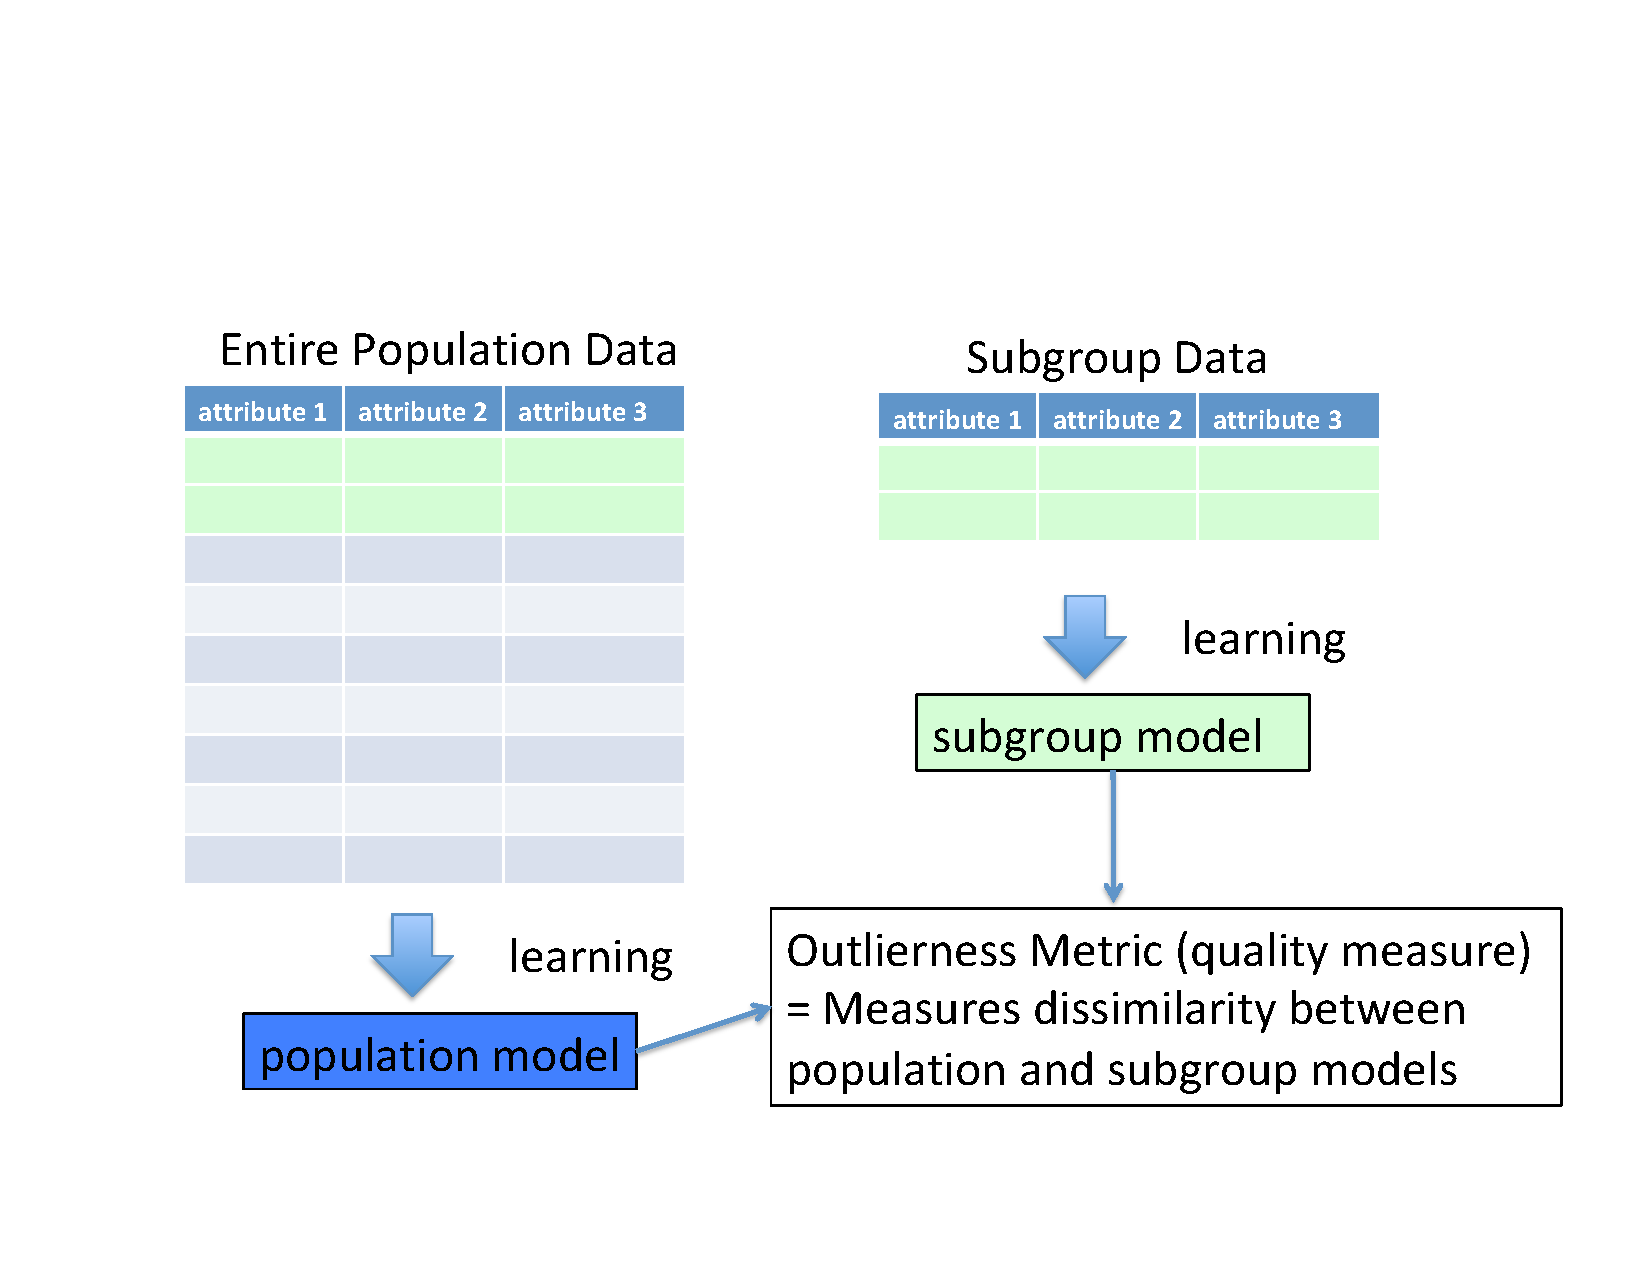
\includegraphics[width=0.7\textwidth]
{emm.pdf}
\caption{A general schema for Exceptional Model Mining  for propositional i.i.d. data
\label{fig:emm}}
\end{figure}

{\em Model Type.} EMM is an inclusive framework in that any model type of interest can be utilized. In this paper we focus on first-order Bayesian networks (BNs)~\cite{Wang2008,Poole2003,Kimmig2014}, but our definitions apply to other log-linear models such as Markov Logic Networks \cite{Domingos2007}. 
A class-model Bayesian network (BN) structure is learned with data for the entire population. The nodes in the BN represent attributes for links, of multiple types, and attributes of objects, also of multiple types. To learn the BN model, we apply techniques from statistical-relational learning, a  recent field that applies and extends AI and machine learning to relational data\cite{SRL2007,Schulte2012,Domingos2009}. For a learned BN structure, we compare two parameter vectors: The class model parameters are estimated from the entire population data, and the object model parameters are estimated from the object data. 
% TODO: we can think of the object model as representing the role of an entity
%The BN provides dimensionality reduction, in the sense that it leverages independencies to represent the data distribution with exponentially fewer parameters than a non-factorized parametrization. 

{\em Quality Measure = Outlierness Metric.} For a given model type, quantifying the extent to which an object model deviates from the population class model is the main research question in EMM~\cite{Duivesteijn2016}. A computational method for measuring this extent is called a quality measure; when we apply EMM to relational outlier detection, we also refer to it as an {\em outlierness metric}. We propose utilizing the relational log-linear likelihood function \cite{Kimmig2014,Schulte2011} that measures how well a parametrized statistical-relational model fits fits an input database. The {\em likelihood ratio} is the difference in log-likelihood between the class model and the object model, when applied to the object data. Assuming maximum likelihood estimates, it is equivalent to the Kullback-Leibler divergence (KLD) between class and object models. While our evaluation indicates that KLD is a good outlierness metric, we propose improving it further by applying two transformations: (1) a mutual information decomposition, and (2) replacing log-likelihood differences by log-likelihood distances. We refer to the resulting novel score as the {\em log-likelihood distance}. 


%
%
%Given a set of parameter values and an input database, it is possible to compute a {\em class model likelihood} that quantifies how well the BN fits the object data. The class model likelihood uses BN parameter values {\em estimated from the entire class data.} This  is a relational extension of the standard log-likelihood method for i.i.d. vectorial data, which uses the likelihood of a data point as its outlier score. %This can be adapted for object-relational data as follows.
%%The Bayes net structure represents the normal pattern of associations among links and attributes  by the well-known d-separation criterion: Two nodes are probabilistically independent if they are d-separated. 
%While the class model likelihood is a good baseline score, it can be improved by comparing it to {\em the object model likelihood}, which uses BN parameter values {\em estimated from the object data.}
%The {\em model log-likelihood ratio} (LR) is the log-ratio of the object model likelihood to the class model likelihood. This ratio quantifies how the probabilistic associations that hold in the general population deviate from the associations in the object data substructure.
%While the 
%likelihood ratio discriminates relational outliers better than the class model likelihood alone, it can be improved further by applying two transformations: (1) a mutual information decomposition, and (2) replacing log-likelihood differences by log-likelihood distances. We refer to the resulting novel score as the {\em log-likelihood distance}.
%
%This paper considers outlier detection for object-oriented data. Object-orientation is one of the main data models for representing structured data~\cite{Ramakrishnan2003,Koller1997}. It is a natural data model for the widely used XML format, where nodes in the XML document tree are viewed as objects.\footnote{\url{http://www.w3.org/DOM/}} 
%%
%%The object-oriented data model was inspired by object-oriented programming. 
%%There are different formulations of the object-oriented data model
%%; the concepts in this paper apply to data objects in general. 
%The main 
%characteristics of data objects that we utilize in this paper are the following. (1) {\em Object Identity.} Each object has a unique identifier that is the same across contexts. For example, a player has a name that identifies him in different matches. (2) {\em Class Membership.} An object is an instance of a class, which is a collection of similar objects. In particular, objects in the same class share a set of attributes. For example, van Persie is a player object that belongs to the class striker, which is a subclass of the  class player. (3) {\em Component Relationships.} Atomic objects have attributes but no components. Complex objects contain other objects as components or parts. For example, a match involves two teams, and each team comprises a set of players for that match. 
%
%%Standard outlier or anomaly detection methods are defined for a data model of atomic objects from the same class without subobjects. 
%%``flat'' feature vectors, which are atomic objects with no subobjects. 
%The class and component hierarchies represent information about objects that an outlier detection method should take into account. We achieve this in two steps. Step 1: the component hierarchy is used to compute an {\em object profile}. The object profile is a data structure that specifies the object's attributes and the attributes of related objects. Two objects are related if there is a chain of components connecting them. For example, for each soccer player, there is a player distribution over: the player's attributes, the player's team's results in matches, and the actions of the player in matches.
%%For example, for each soccer team, there is a team distribution over: the team's attributes, the team's results in matches, and the actions of the team's players in matches. 
%Step 2: Given a set of object profiles, compute an outlier score that measures how the object's profile differs from the profiles of other objects in its class. We develop a probabilistic approach where:
%
%\begin{quote}
%	Object Outlier Score = Score between object distribution and class distribution
%\end{quote}
%
%For each object, the object distribution is a joint distribution over the object's attributes and the attributes of related objects. The object distribution can be computed from counts in the object profile. The class distribution is the distribution of a randomly chosen object in the class. 
%
%
%%
%This approach allows us to apply ideas from the well-researched topic of probability divergences to the problem of object outlier detection. A baseline divergence concept is the standard Kullback-Leibler divergence (KLD). KLD computes the expected log-{\em difference} between two joint distributions. Our argument in this paper is that for outlier detection, we ought to use instead the expected log-{\em distance} between two joint distributions. The reason is that averaging distribution differences loses information when two distribution differences point in opposite directions, and cancel each other out. We refer to our novel divergence as the expected log-distance divergence (ELD).
%%\vspace{-5mm}
\paragraph{Evaluation} Our code and datasets are available on-line at \cite{url}. We evaluate relational EMM outlierness metrics in three ways.

{\em Detection Accuracy.} Our performance evaluation follows the design of previous outlier detection studies~\cite{Gao2010,aggarwal2013},
%~\cite{Cansado2008, Muller2012},
%\footnote{review} 
where the methods are scored against a test set of known outliers.  
%and case studies assess their output on specific cases. 
%
We use three synthetic and four real-world datasets, from the UK Premier Soccer League, the Internet Movie Database (IMDb), the National Hockey League, and Mutagenesis. On the synthetic data we have known ground truth. For the real-world datasets, we use a one-class design, where one object class is designated as normal and objects from outside the class are the outliers. For example, we compare goalies as outliers against the class of strikers as normal objects. 
%Given ground truth, an outlier detection method can be scored in terms of true positives and negatives, summarized using AUC~\cite{Muller2012}.\footnote{review} 
%Comparisons outlier scores include the class model likelihood, our novel log-likelihood distance, and likelihood-based scores intermediate to these two. 
%Previous outlier analysis for similar structured data  \cite{Breunig2000} used a preprocessing step where the structured data are converted to vectorial data that represent atomic objects. This conversion is usually done by aggregation, which tends to lose information.
%, for instance using counts as attributes in an attribute vector. After aggregation, we evaluate 
%After aggregation, standard outlier detection methods for independent data points can be applied; we use three as baseline methods for our evaluation ($\outrank$, $\lof$, and $\knn$).
Compared to six baseline methods, the EMM-based scores (likelihood ratio and log-likelihood distance) achieve the top detection accuracy on all three synthetic datasets, and on 4 out of 5 real-world datasets.

{\em Case Studies.} We also offer case studies where we assess whether individuals that our score ranks as highly unusual in their class are  indeed unusual. 
%This assessment looks at the object profile data of these individuals. 
The case studies illustrate that the EMM scores are {\em easy to interpret}, because the Bayesian network provides a local decomposition of log-likelihood differences. Interpretability is very important for users of an outlier detection method as there is often no ground truth to 
evaluate outliers.% suggested by the method.

{\em Correlation with Success.} We compare the likelihood-based outlierness metrics to independent success metrics for a given domain. Success rankings are one of the most interesting features to users. Our reasoning is that high success is an independent metric that indicates an unusual individual. So a correlation between an outlierness metric and success is an independent validation of the meric, and also shows that it points to meaningful and interesting outliers.

 %With regards to the cost of computing the divergence outlier score, we show that a Bayesian network representation of the object distributions can speed up the computation by orders of magnitude.

%One of our baseline methods is a variant of the distribution divergence approach that we introduce in this paper, where Kullback-Leibler convergence is the used as the outlier score. 
%
%we rank both normal and outlier individuals against the distribution of the normal class only. For example, we 
%compare the attribute distributions of both goalies and strikers against the class distribution of strikers. 
%
%We compare the detection accuracy of our novel mutual information divergence with the Kullback-Leibler convergence.
%basing a distribution divergence on the expected distance to basing it on the expected difference. 
%As regards to previous methods, to our knowledge ours is the first outlier detection method tailored for object-oriented data. Previous outlier analysis for structured data similar to ours (e.g., sports data) \cite{Breunig2000} used a preprocessing step where the structured data are converted to a matrix of attribute vectors that represent atomic objects. 
%  outlier detection methods for the atomic objects data model---based  on a single data matrix---have been applied to datasets similar to those that we examine  
% previously analyzed with 
%Standard outlier detection methods require as input a data matrix, that represents attributes of atomic objects from the same class. It is therefore not possible to provide structured data as input directly to such methods. In previous outlier detection work, data matrix methods were applied by 
%Converting object-oriented data to a data matrix can be done by aggregation.
%, for instance using counts as attributes in an attribute vector. After aggregation, we evaluate 
%After aggregation, standard outlier detection methods for independent data points can be applied; we use three as baseline methods for our evaluation ($\outrank$, $\lof$, and $\knn$).
% three aggregation approaches  using a subspace outlier ranking method, $\outrank$, a density-based outlier detection method, the Local Outlier Factor ($\lof$), and a distance based outlier detection method, $\knn$.  On all datasets, the log-distance divergence achieves the best detection accuracy.
%We also offer case studies where we discuss why highly ranked individuals are indeed unusual in their class. The case studies illustrate that our divergence outlier score is easy to interpret, because it is based on a sum decomposition of the joint distributions. Interpretability is very important for users of an outlier detection method as there is often no ground truth to 
%evaluate outliers indicated by the method. 
%\vspace{-5mm}
\paragraph{Contributions} Our main contributions may be 
summarized as follows.

\begin{enumerate} 
	\item The first approach to outlier detection for structured relational data that is based on a probabilistic model, applying the EMM framework.
	\item A new model-based outlier score based on a novel model likelihood comparison, the log-likelihood distance.  % \footnote{Commented paper organization}
\end{enumerate}
% \vspace{-0.5cm} 
				
				\paragraph{Previous Conference Publication.} A preliminary version of this paper appeared in the Proceedings of the IEEE SSCI series \cite{Riahi2015} (Best Student Paper). The new material in this submission comprises the following:
				
				\begin{enumerate} 
				\item We expanded and clarified the relationship to previous work in EMM.
					\item We added new experiments on the real-world datasets.
					\item We performed a comparison between our proposed metric and a well-known relational-based distance learning method ($\textit{RIBL}$).
					\item We introduced an application of the proposed metrics in detecting outstanding individuals and ranking them.
					\item We applied Taylor series analysis to understand analytically the relationship between the log-likelihood ratio and the log-likelihood distance (the former is approximated by $\chi^{2}$, the latter by L1 norm). 
				  % \footnote{Commented paper organization}
				\end{enumerate}

\paragraph{Paper Organization} We review related work on outlier detection for structured data, then background about Bayesian networks for relational data. Then we introduce likelihood-ratio based outlierness scores for relational EMM, including our novel log-likelihood distance. 
%After presenting the details of our approach, we review related work. 
Empirical evaluation compares EMM and aggregation-based approaches to relational outlier detection, with respect to three synthetic and four real-world datasets.

				\section{Related Work}
				Outlier detection is a densely researched field, for a survey please see~\cite{aggarwal2013,Akoglu2015}.
				Figure~\ref{fig:novelty} provides a tree picture of where our method is situated with respect to other outlier detection methods and other data models. 
				%For an outlier detection survey please see~\cite{aggarwal2013}.
				%\cite{Hodge2004,aggarwal2013}. 
				Our method falls in the category of {\em unsupervised} statistical model-based approaches. To our knowledge, ours is the first model-based method tailored for object-relational data. Like EMM and other model-based approaches, it detects {\em global outliers.} Aggarwal \cite{aggarwal2013} defines a global outlier to be a data point that notably deviates from the rest of the population. We review relevant approaches from different data models, the most common atomic object model---where data is represented by vectors---and structured data models.\\
				
				% using the XML, SQL, and OLAP formats.
				%\vspace{-5mm}
				\textit{a) Attribute Vector Data Model:}
				%\footnote{\textbf{Sarah}: can you fix the silly d) for paragraph numbering?}By far most work on outlier detection considers atomic objects with flat feature vectors.
				By far most work on outlier detection considers atomic objects with flat feature vectors.
				%, or nonhierarchical structures like time series. 
				This leads to an impedance mismatch: 
				The required input format for these outlier detection methods is a single data matrix, not a structured dataset. For example, one cannot provide a relational database as input. This mismatch is not simply a question of choosing a file format, but instead reflects a different underlying data model: complex objects with both attributes and component objects vs. atomic objects with attributes only. 
				%
				It is possible to ``flatten'' structured data by converting it to unstructured feature vectors, for instance by using aggregate functions. 
				%Flattening incurs some loss of information but allows us to apply the many feature vector methods.
				%\cite{Elke2013}. 
				We evaluated the aggregation approach in this paper by applying three standard methods for outlier detection.
				%for three major approaches to outlier detection: distance-based, density-based, and subspace clustering. 
				%
				%Subspace clustering methods (e.g., \cite{Muller2012,Kriegel2009}) are similar to our work in the sense that they aim to decompose a complex data space. They find complex deviations that are noticeable only in a data subspace. A common approach is to discover datapoints that show unexpected deviations in similar subspaces. Our approach instead develops a joint measure of how dissimilar the target object profile distribution is to the class distribution over the entire data space. Given that object and class distributions are represented by an object-oriented Bayesian network \cite{Koller1997}, the network structure defines subspaces. The joint divergence measure {\em mathematically decomposes} into subspace measures that quantify how dissimilar the target object profile distribution is in the subspaces defined by the network, compared to the class distribution in the same subspace.
				
				Work on atomic contextual  outliers \cite{Tang2013} is like ours in that it considers the distinctness of a target individual from a reference class. A reference class is not specified for each object,
				%as a property of the object, 
				but is constructed as part of outlier detection. 
				Our work could be combined with a class discovery approach by providing a score of how informative the inferred classes are. 
				\begin{figure}
					\centering
					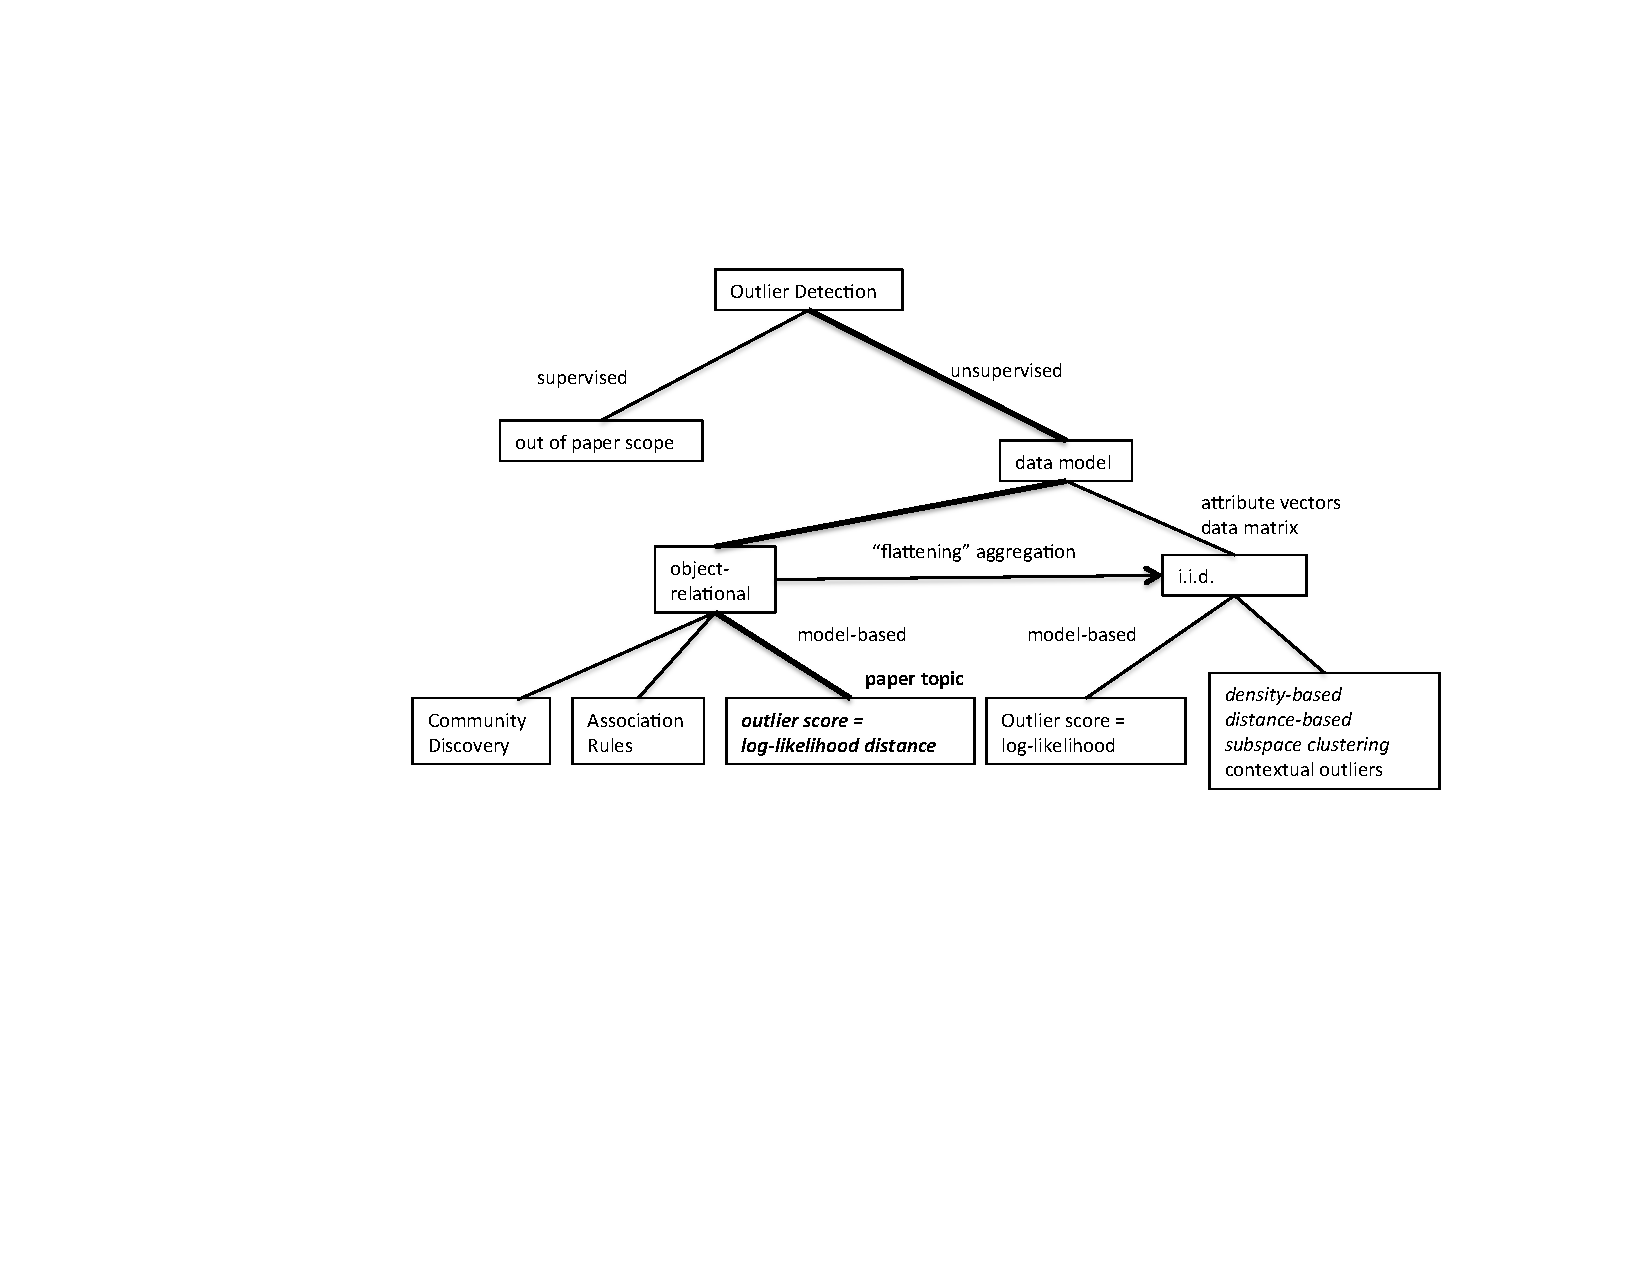
\includegraphics[width=1\textwidth] {NoveltyDiagram.pdf}
					\caption{A tree structure for related work on outlier detection for structured data. A path specifies an outlier detection problem, the leaves list major approaches to the problem. Approaches in italics appear in experiments.
						\label{fig:novelty}}
				\end{figure}
				%\vspace{-5mm}
				
				\textit{b) Structured Data Models:} We discuss related techniques in three types of structured data models: SQL (relational), XML (hierarchical), and OLAP (multi-dimensional). 
				
				For relational data, many outlier detection approaches aim to discover rules that represent the presence of anomalous associations for an individual or the absence of normal associations \cite{Maervoet2012,Gao2010}.    In these approaches what we call the object data is usually referred to as an interpretation, so the problem is to score outlier interpretations~\cite{Maervoet2012}. The survey by \cite{Novak2009} unifies within a general rule search framework related tasks such as exception mining, which looks for associations that characterize unusual cases, subgroup mining, which looks for associations  characterizing important subgroups, and contrast space mining, which looks for differences between classes. Another rule-based approach uses Inductive Logic Programming techniques \cite{Angiulli2007}.
				%,Angiulli2009}.
				While local rules are informative, they are not based on a global statistical model and do not provide a single outlier score for each individual. As we show in our case studies (Section~\ref{sec:CaseStudy}), the conditional probability parameters in a Bayesian network can be used to extract rules  from the BN model (of the form $\it{parent\_values} \rightarrow \it{child\_value}$).
				The Distance-based algorithms designed for outlier detection can be applied to the relational case.  Horvath {\em et al.} introduced a similarity measure for the first-order instance-based learner RIBL that uses the edit distance to compute the distance between lists and terms~\cite{Horvath2001}. This distance has been used for the clustering task in~\cite{Kirsten2001}. To the best of our knowledge, distance-based relational learning has not been used for outlier detection. One-class classification can be viewed as a special case of outlier detection.  Khot {\em et al.} introduced a non-parametric relational one-class classification based on first-order trees. They proposed a tree-based distance metric to discover new relational features and to differentiate relational examples~\cite{Khot2014}. Khot {\em et al.} emphasize that their method is not appropriate for outlier detection because outlier detection makes different assumptions about the data than they do (e.g. outliers are far and isolated).  
				
				 Propositionalization summarizes the multi-relational data into a single data table and can be used for outlier detection and classification tasks~\cite{Kramer2000,Lavrac13,kuzelka2008,Riahi2016,AndersonP08}. 
				
				A latent variable approach in information networks ranks potential outliers in reference to the latent communities inferred by network analysis \cite{Gao2010}. Our model also aggregates information from entities and links of different types, but does not assume that different communities have been identified. 
				
				
				Koh {\em et al.}~\cite{Koh2008} propose a method for hierarchical structures represented in XML document trees. Their aim is to identify feature outliers, not class outliers as in our work. Also, they use aggregate functions to convert the object hierarchy into feature vectors. Their outlier score is based on local correlations, and they do not construct a model.
				
				
				The multi-dimensional data model defines numeric measures for a set of dimensions. 
				%A seminal approach to exploring a multi-dimensional datacube was presented by Sarawagi {\em et al.}~\cite{Sarawagi1998}. 
				%The object and the multi-dimensional data models are similar in the respect that both objects and dimensions are ordered in a hierarchy. However, 
				The differences in the two data models mean that multi-dimensional outlier detection models~\cite{Sarawagi1998} do not carry over to object-relational outlier detection. (1) The object data model allows but does not require any numeric measures. In our datasets, all features are discrete. Nor do we assume that it is possible to aggregate numeric measures to summarize lower-level data at higher levels.  
				(2) In scoring a potential outlier object, our method considers other objects {\em both} below and above the target object in the component hierarchy. OLAP exploration methods consider only cells below or at the same level as the target cell. For example, in scoring a player, our method would consider features of the player's team.  
				Also, the log-likelihood distance outlier score of an object is not determined by the outlier scores of its components, in contrast to approaches derived from Sarawagi {\em et al.}~\cite{Sarawagi1998}. They use values such as the most unusual cell that is below a target cell.
				(3) Our approach models a joint distribution over features, exploiting correlations among features. Most of the OLAP-based methods consider only a single numeric measure at a time, not a joint model.  




\section{Background: Bayesian Networks for Relational Data}
We adopt  
the Parametrized Bayesian network (PBN) formalism \cite{Poole2003} that combines Bayesian networks with logical syntax for expressing relational concepts. 


\subsection{Relational Data}




%We apply the learn-and-join algorithm (LAJ), which is the state-of-the-art Bayes net learning method for relational data. The LAJ algorithm takes as input a relational database and outputs a Bayes net using the functor notation due to Poole \cite{Poole2003}. We briefly review this notation.

%\paragraph{Functor Terms} 
We adopt a term-based notation for combining logical and statistical concepts~\cite{Poole2003,Kimmig2014}. {Table~\ref{table:notation} summarizes our notation.
A functor is a function or predicate symbol. Each functor has a set of values (constants) called the \textbf{domain} of the functor. The range of a \textbf{predicate} is $\{\true,\false\}$. Predicates are usually written with uppercase Roman letters, other terms with lowercase letters.
A predicate of arity at least two is a \textbf{relationship} functor. Relationship functors specify which objects are linked. Other functors represent \textbf{features} or \textbf{attributes} of an object or a tuple of objects (i.e., of a relationship).
A \textbf{population} is a set of objects. 
A \textbf{term} is of the form $f(\term_{1},\ldots,\term_{k})$ where $\functor$ is a functor %(either a function symbol or a predicate symbol) 
and each $\term_{i}$ is a first-order variable or a constant denoting an object. A term is \textbf{ground} if it contains no first-order variables; otherwise it is a first-order term. In the context of a statistical model, we refer to first-order terms as \textbf{Parametrized Random Variables} (PRVs) \cite{Kimmig2014}. 
%A term whose range are the truth values $\{\true,\false\}$ is a \textbf{predicate}. 
%Predicates are usually written with uppercase Roman letters, other term with lowercase letters.
%The grounding concept represents moving from the population-level  to the object level. 
A \textbf{grounding} replaces each first-order variable in a term by a constant; the result is a ground term. A grounding may be applied simultaneously to a set of terms.  A relational database $\D$ specifies the values of all ground terms. %, which can be listed in data tables. 
%In machine learning terminology, the data tables are contingency tables that represent sufficient statistics or event counts.

Consider a joint assignment 
$P(\Features = \set{\nodevalue})$ of values to a set of PRVs $\Features$. The {\em grounding space} of the PRVs is the set of all possible grounding substitutions, each applied to all PRVs in $\Features$. The {\em count} of groundings that satisfy the assignment with respect to a database $\D$ is denoted by $\grounds_{\D}(\Features = \set{\nodevalue})$. The \textbf{database frequency} $P_{\D}(\Features = \set{\nodevalue})$ is the grounding count divided by the number of all possible groundings. %Table~\ref{table:notation} contains a complete set of notations used in this paper.
%, that is, the size of the grounding space.
 	 	      \begin{table} 
 	 	     
 	 	      	\centering
 	 	      	\resizebox{1\textwidth}{!}{
 	 	      		\begin{tabular}{|l|l|}
 	 	      			\hline
 	 	      			Symbol&Definition\\\hline
 	 	      			$\a,\b,\a_{1},\b_{1},\ldots$ & Constant \\\hline
 	 	      			$\A,\B,\it{T},\it{M},\ldots$ & First-order variable
 	 	      			\\\hline $\functor,g,\ldots,$ & Functor, function symbol
 	 	      			\\\hline
 	 	      			$\functor(\A,\ldots,\A_{k})$& First-order term\\\hline
 	 	      			$\functor(\A=\a_{1},\ldots,\A_{k}=\a_{k})$ & Ground term \\\hline
 	 	      			$\D$& Relational database\\\hline
 	 	      			$\D_{\Class}$ &Database for the entire class of objects\\\hline
 	 	      			$\D_{\object}$& Restriction of the input database to the target object\\\hline
 	 	      			$\feature(\A,...,\B)$& A parametrized random variable\\\hline
 	 	      			$\Features $&A set of first-order random variable\\\hline
 	 	      			%  $\{\nodevalue_{i1},\ldots,\nodevalue_{i\states_{i}}\}$&Possible values of $\feature_{A,B,...}$\\\hline
 	 	      			$\Features = \set{\nodevalue}$& Joint assignment of values to a set of PRVs\\\hline
 	 	      			$P(\Features = \set{\nodevalue}) \equiv P(\set{\nodevalue})$ &Joint probability that each variable $\feature_{i}$ takes on value $\set{\nodevalue}_{i}$\\\hline
 	 	      			$\grounds_{\D}(\Features = \set{\nodevalue})$& Count of groundings that satisfy the assignment\\\hline
 	 	      			
 	 	      			$\A$\textbackslash$v$& Ground a first-order variable\\\hline
 	 	      			
 	 	      			$\model$&A Bayesian network structure\\\hline
 	 	      			$\model_{\Class}$ & A Bayesian network structure learned with $\D_{\Class}$ as the input database\\\hline
 	 	      			$\parameters_{\Class}$ & Parameters learned for $\model_{\Class}$ using $\D_{\class}$  as the input database\\\hline
 	 	      			$\parameters_{\object}$ & Parameters learned for $\model_{\Class}$ using $\D_{\object}$  as the input database\\\hline
 	 	      			$\parents_{i}$&Parent of node $i$\\\hline
 	 	      			% $\parameters_{\object}$ are parameters learned for $\model_{\Class}$ using $\D_{\class}$ resp. $\D_{\object}$ as the input database.
 	 	      			%Synthetic&40&280\\ \hline
 	 	      		\end{tabular}} 	\caption[Table of Notations]{Notation and Definition	\label{table:notation}}
 	 	      	\end{table}\\
\emph{Example.} \label{sec:example}
%
The Opta dataset represents information about Premier League data %\cite{opta-original} 
(Sec.~\ref{sec:real}). 
%Using the functor notation, the data
%format can be represented as follows. 
The basic populations are teams, players, matches, with 
corresponding first-order variables $\team, \player, \match$. As shown in Table~\ref{table:data}, the groundings count can be visualized in terms of a groundings table ~\cite{Schulte2012}, also called a universal schema~\cite{Riedel2013}. 
%Table~\ref{table:data} specifies values for some ground terms. 
The first three column headers show first-order variables ranging over different populations. The remaining columns represent terms. Each row represents a single grounding and the values of the ground terms defined by the grounding.
%Table~\ref{table:counts} illustrates grounding counts. 
In terms of the grounding table, the grounding count of a joint assignment is the number of rows that satisfy the conditions in the joint assignment. The database frequency is the grounding count, divided by the total number of rows in the groundings table. Table~\ref{table:counts} shows example of computing frequencies. Counts are based on the 2011-2012 Premier League Season. We count only groundings $(\it{team},\it{match})$ such that $\it{team}$ plays in $\it{match}$. Each team, including Wigan Athletics, appears in 38 matches. The total number of team-match pairs is $38 \times 20 = 760$.

%Examples of terms include the following. 

%\begin{itemize}
%\item $\it{Appears\_Player}(\P,\M)$ indicates whether a player appeared in a match.
%\item $\it{Appears\_Team}(\T,\M)$ indicates whether a team played in a match.
%\item $\it{Team}(\P)$ returns the team of a player.
%\item $\it{Result}(\T,\M)$ denotes the result of a team in a match (win or lose).
%\item $\it{ShotEff}(\T,\M)$ denotes the shot efficiency of a team in a match (number of successful shots on target, per total number of shots).
%\item $\it{TimePlayed}(\P,\M)$ denotes the total time that a player played in a match.
%\end{itemize}


%\begin{table}[htbp]
%\caption{Examples of terms in the soccer dataset.}
%\centering
%\resizebox{1\textwidth}{!}{
%\begin{tabular}{|c|p{5cm}|}
%\hline
%Term&Meaning\\ \hline
%$\it{Appears\_Player}(\P,\M)$ & indicates whether a player appeared in a match.\\ \hline
%$\it{Appears\_Team}(\T,\M)$&indicates whether a team played in a match.\\ \hline
%$\it{Team}(\P)$& returns the team of a player.\\ \hline
%$\it{Result}(\T,\M)$ &denotes the result of a team in a match (win or lose).\\ \hline
%$\it{ShotEff}(\T,\M)$ &denotes the shot efficiency of a team in a match (number of successful shots on target, per total number of shots).\\ \hline
%$\it{TimePlayed}(\P,\M)$& denotes the total time that a player played in a match.\\ \hline
%\end{tabular}}
%\label{table:terms}
%\end{table}

\begin{table}[htbp]

	\centering
	\resizebox{1\textwidth}{!}{
		\begin{tabular}{|c|c|l|c|c|c|}
			\hline
			\multicolumn{1}{|l|}{MatchId \match} &
			TeamId \team & PlayerId \player
			& \multicolumn{1}{l|}{TimePlayed(\player,\match)} & 
			\multicolumn{1}{l|}{ShotEff(\team,\match)}&result(\team,\match) \\ \hline
			117 & WA & McCarthy  & 90 & 0.53&\it{win}\\ \hline
			148 & WA & McCarthy  & 85 & 0.57&\it{loss}\\ \hline
			15 & MC & Silva  & 90 & 0.59&\it{win}\\ \hline
			\ldots& \ldots &\ldots&\ldots&\ldots&\\
		\end{tabular}}	\caption{Sample Population Data Table (Soccer). \label{table:data}}

		\resizebox{1\textwidth}{!}{
			\begin{tabular}{|c|c|l|c|c|c|}
				\hline
				\multicolumn{1}{|l|}{MatchId \match} &
				TeamId $\team = \it{WA}$ & PlayerId \player& \multicolumn{1}{l|}{TimePlayed(\player,\match)} & 
				\multicolumn{1}{l|}{ShotEff(\it{WA},\match)}&result(\it{WA},\match) \\ \hline
				117 & WA & McCarthy  & 90 & 0.53&\it{win}\\ \hline
				148 & WA & McCarthy  & 85 & 0.57&\it{loss}\\ \hline
				\ldots& WA &\ldots&\ldots&\ldots&\\
			\end{tabular}}		\caption{Sample Object Data Table, for team $\team = \it{WA}$. \label{table:individual}}
		\end{table}
		
		
		
		
		A novel aspect of our paper is that we learn model parameters for specific objects as well as for the entire population. 
		%To implement this, for each target object, we form 
		The appropriate \textbf{object data table} is formed from the population data table by restricting the relevant first-order variable to the target object. 
		For example, the object database for target Team $\it{Wigan Athletic}$, 
		forms a subtable of the data table of Table~\ref{table:data} that contains only rows where 
		TeamID = $\it{WA}$; see Table~\ref{table:individual}. In database terminology, an object database is like a view centered on the object.
		
		%\begin{table} 
		%	\captionsetup{singlelinecheck=off}
		%			\caption[.]{\label{table:counts}Example of Grounding Count and Frequency for the conjunction \begin{displaymath} \it{passEff(T,M)=hi}, shotEff(T,M)=high, Result(T,M)=1.\end{displaymath}}
		%			\centering
		%			\resizebox{1\textwidth}{!}{
		%				\begin{tabular}{|c|c|c|}
		%					\hline
		%					Database&Count or $\#_{D}(\Features = \set{\nodevalue})$&Frequency or $P_{D}(\Features = \set{\nodevalue})$\\\hline
		%					Population&76& $76/760=0.10$\\\hline
		%					Wigan Athletics&7&$7/38=0.18$\\\hline
		%		
		%					%Synthetic&40&280\\ \hline
		%				\end{tabular}}
		%			\end{table}
		\begin{table} 

			\centering
			\resizebox{1\textwidth}{!}{
				\begin{tabular}{|c|c|c|}
					\hline
					Database&Count or $\#_{D}(\Features = \set{\nodevalue})$&Frequency or $P_{D}(\Features = \set{\nodevalue})$\\\hline
					Population&76& $76/760=0.10$\\\hline
					Wigan Athletics&7&$7/38=0.18$\\\hline
					
					%Synthetic&40&280\\ \hline
				\end{tabular}}			\caption{Example of Grounding Count and Frequency in Premier League Data, for the conjunction $\it{passEff(T,M)=hi}, shotEff(T,M)=hi, Result(T,M)=win$.\label{table:counts}}
			\end{table}
			
			%\begin{table} 
			%	\captionsetup{singlelinecheck=off}
			%			\caption[.]{\label{table:counts}Example of Grounding Count and Frequency for the conjunction \begin{displaymath} \it{passEff(T,M)=hi}, shotEff(T,M)=high, Result(T,M)=1.\end{displaymath} Counts are based on the 2011-2012 Premier League Season. We count only groundings $(\it{team},\it{match})$ such that $\it{team}$ plays in $\it{match}$. Each team, including Wigan Athletics, appears in 38 matches. The total number of team-match pairs is $38 \times 20 = 760$.
			%			\label{MetricComputation}}
			%			\centering
			%			\resizebox{1\textwidth}{!}{
			%				\begin{tabular}{|c|c|c|}
			%					\hline
			%					Database&Count or $\#_{D}(\Features = \set{\nodevalue})$&Frequency or $P_{D}(\Features = \set{\nodevalue})$\\\hline
			%					Population&76& $76/760=0.10$\\\hline
			%					Wigan Athletics&7&$7/38=0.18$\\\hline
			%		
			%					%Synthetic&40&280\\ \hline
			%				\end{tabular}}
			%				
			%			\end{table}
			
			%[Example of counts, frequencies]
			% For simplicity only, suppose that the only matches and players in the season are those shown in Table~\ref{table:data}. Then the attribute value $\it{First\_goals} = 0$ occurs with frequency $1/2$ in the object distribution $P_{\it{si}}$ for Silca. In the player class distribution $P_{\it{Player}}$, the attribute value $\it{First\_goals} = 0$ occurs with frequency $4/5$. So Silva is somewhat less likely to score no goal than a randomly selected player.
			

\subsection{Bayesian Networks}

A Bayesian network (BN) structure $\model$ is a Directed Acyclic Graph (DAG)  whose nodes comprise a set of random variables \cite{Pearl1988}. Depending on context, we interchangeably refer to the nodes  and variables of a BN. Fix a set of variables $\Features = \{\feature_{1},\ldots,\feature_{n}\}$. 
%These are attributes of objects, which can and typically do belong to different classes. In statistical terms, each attribute defines a random variable. 
The possible values of $\feature_{i}$ are enumerated as $\{\nodevalue_{i1},\ldots,\nodevalue_{i\states_{i}}\}$. The notation $P(\feature_{i} = \nodevalue)\equiv P(\nodevalue)$ denotes the probability of variable $\feature_{i}$ taking on value $\nodevalue$. We also use the vector notation $P(\Features = \set{\nodevalue}) \equiv P(\set{\nodevalue})$ to denote the joint probability that each variable $\feature_{i}$ takes on value $\set{\nodevalue}_{i}$. 


The conditional probability parameters of a Bayesian network specify the distribution of a child node given an assignment of values to its parent nodes. For an assignment of values to its nodes, a BN defines the joint probability as the product of the conditional probability of the child node value given its parent values, for each node in the network. This means that the log-joint probability can be {\em decomposed} as the node-wise sum

\begin{equation} \label{eq:bn}
\ln P(\Features = \set{\nodevalue};\model,\parameters) = \sum_{i=1}^{n} \ln \parameter(\set{\nodevalue}_{i}|\set{\nodevalue}_{\parents_{i}})
\end{equation}

\noindent where $\set{\nodevalue}_{i}$ is the assignment of values to node $\feature_{i}$, and $\set{\nodevalue}_{\parents_{i}}$  is the assignment of values to the parents of $\feature_{i}$, as determined by the assignment $\set{\nodevalue}$. 
%The function $\ln$ is the binary logarithm base 2. 
To avoid difficulties with $\ln(0)$, here and below we assume that joint distributions are positive everywhere. Since the parameter values $\parameters$ for a Bayesian network define a joint distribution over its nodes, they therefore entail a marginal, or unconditional, probability for a single node. We denote the \textbf{marginal probability} that node $\feature$ has value $\nodevalue$ as $P(\feature = \nodevalue;\model,\parameters) \equiv \parameter(\nodevalue)$. In the following we use the term Bayesian network model to refer to a network structure with parameters (i.e., a pair $(\model,\parameters)$); for brevity, we also use the terms ``Bayesian network'' or ``model''. 

\paragraph{Example.} Figure~\ref{fig:bn-imdb} shows an example of a Bayesian network model and associated conditional and marginal probabilities. 

\begin{figure}[t]
 		\centering
 		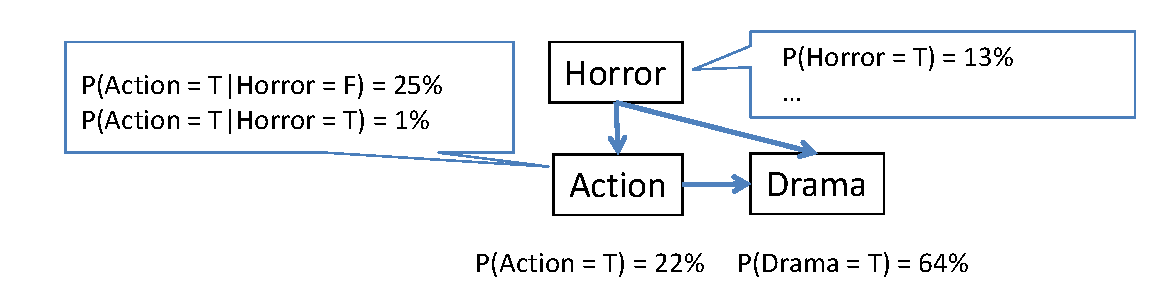
\includegraphics[width=1\textwidth] 
 		{movie-bn.pdf}
 		\caption[Example of conidtional and marginal probabilities computed from a toy Bayesian network structure. ]{Example of joint and marginal probabilities computed from a simple Bayesian network structure that was learned from the $\it{Movies}$ table in the IMDb dataset described in Section~\ref{sec:real}. The parameters were estimated from the  IMDb dataset. The conditional probability parameters for the $\it{Drama}$ node are not shown. The Bayesian  network shows that movie genres are largely but not completely exclusive. For instance, among horror movies, only 1\% are also classified as action movies. The marginal probabilities are the base rate frequencies of horror, action, and drama movies, which are respectively 13\%, 22\%, 64\%.
 			%We show only the Markov blanket of the Results node to simplify. 
 			\label{fig:bn-imdb}
 		}
 	\end{figure}


%

%				\begin{figure}
%				\centering
%				\resizebox{0.9\textwidth}{!}{
%				
%				\subfigure{
%				  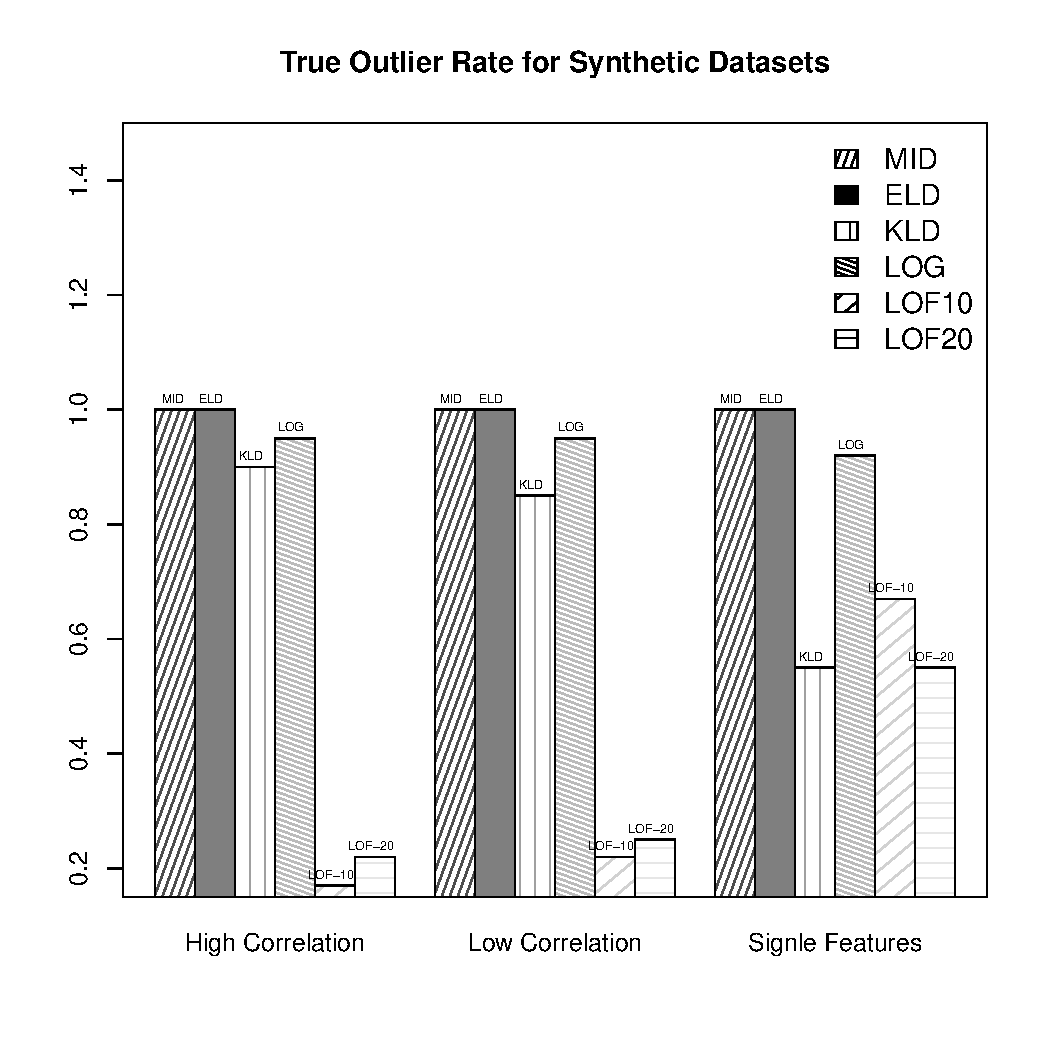
\includegraphics[height=70mm, width=70mm] {figures/TPR-Synthetic.pdf}
%				}
%				\subfigure{
%				  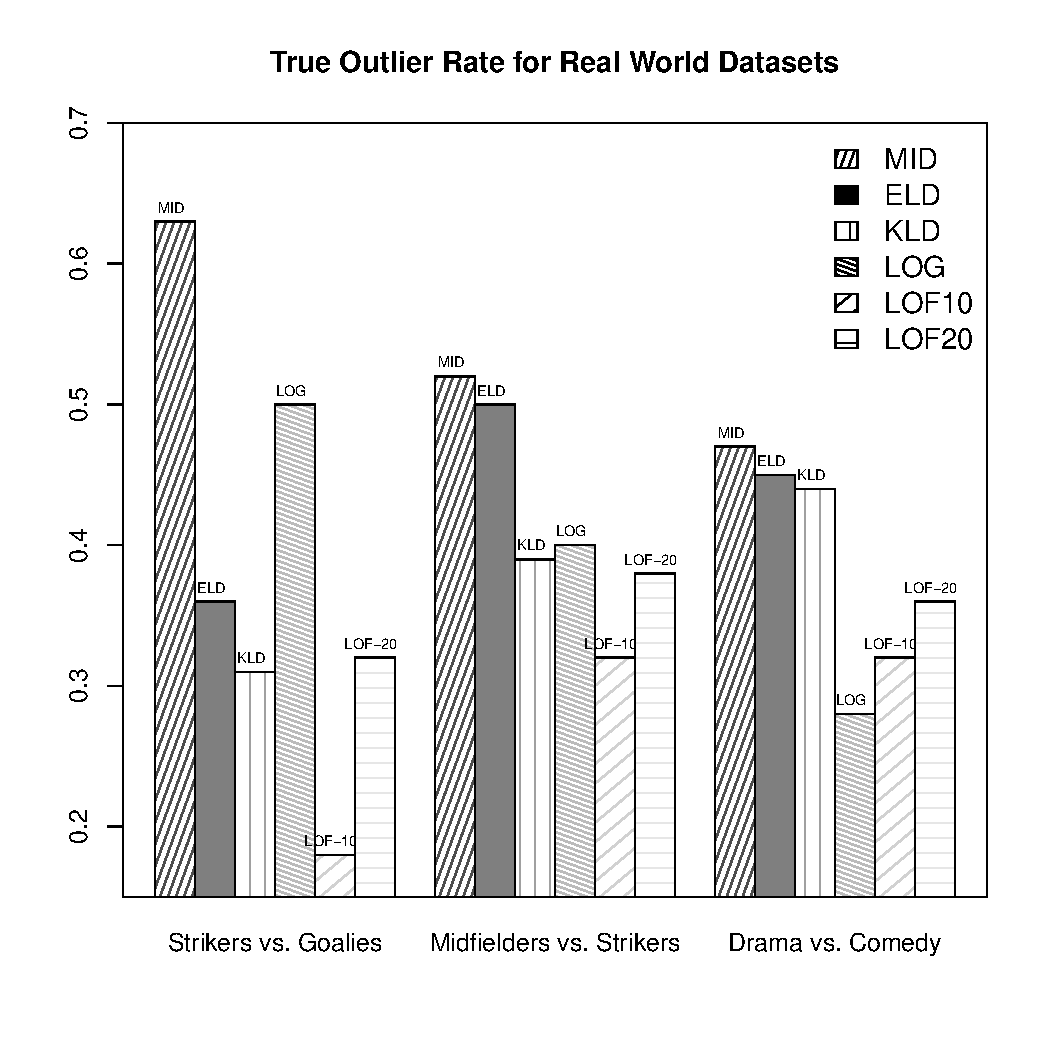
\includegraphics[height=70mm, width=70mm] {figures/TPR-All.pdf}
%				
%				 }
%				 }
%				
%				\caption{Comparison of Object Outlier Metrics}
%				\label{fig:synthetic}
%				\end{figure}
%				

%				\begin{figure}
%					\centering
%					\begin{subfigure}{0.4\textwidth}
%						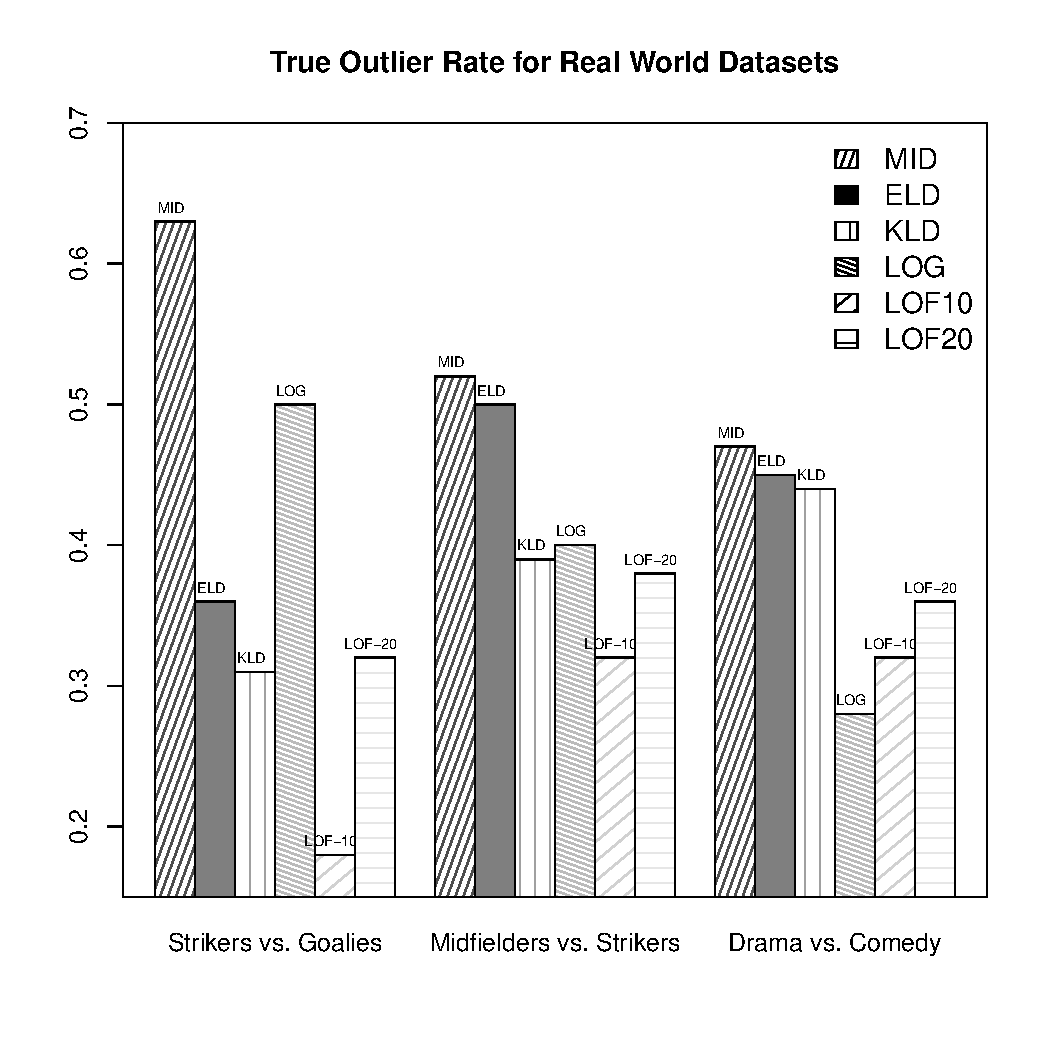
\includegraphics[width=1\linewidth]{figures/TPR-All.pdf}
%						\caption{}
%						\label{fig:Ng1} 
%					\end{subfigure}
%					
%					\begin{subfigure}{0.4\textwidth}
%						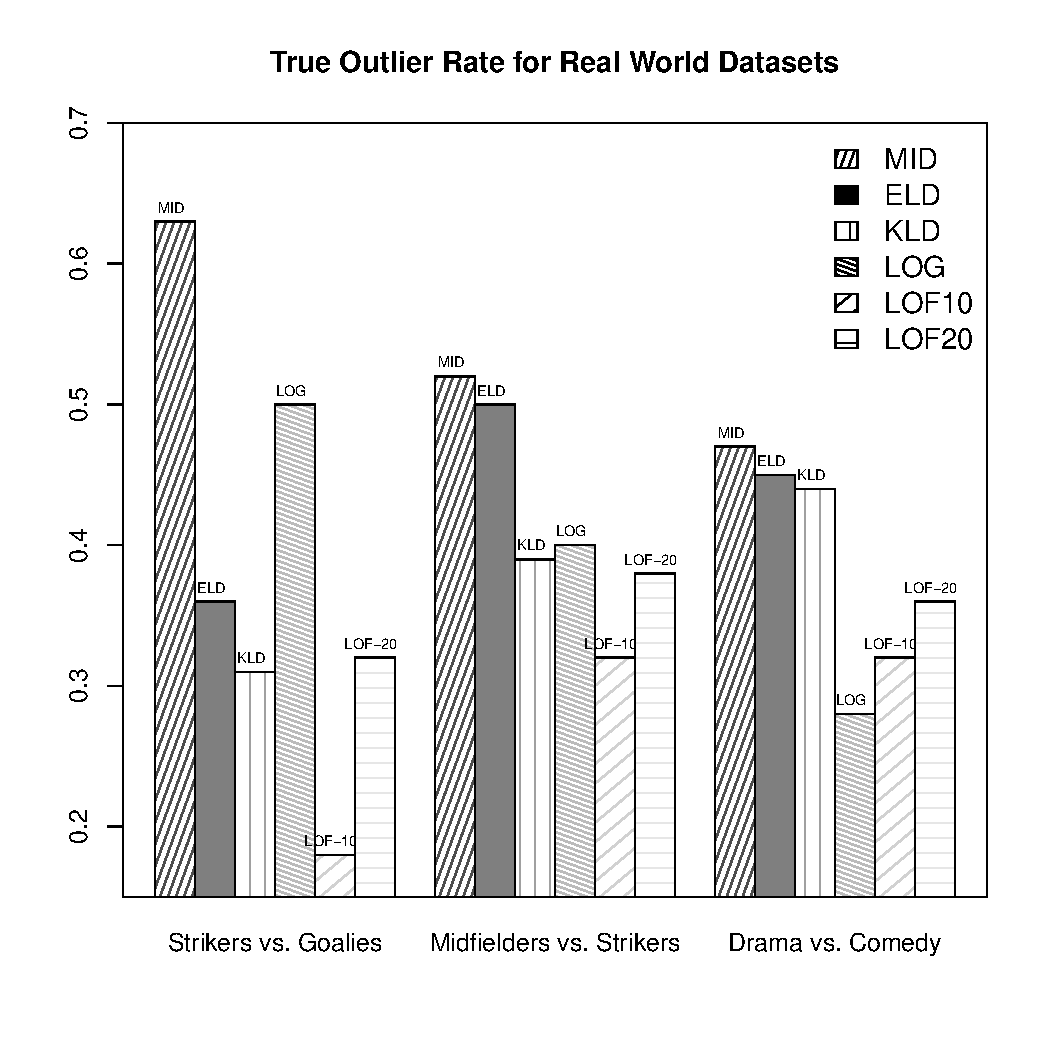
\includegraphics[width=1\linewidth]{figures/TPR-All.pdf}
%						\caption{}
%						\label{fig:Ng2}
%					\end{subfigure}
%					
%					\caption[Two numerical solutions]{(a) Numerical solutions for the small-time system 
%						with a constant-curvature body shape showing the scaled leading-order veritcal 
%						reaction force $N_0$ versus the scaled body mass $M$ for various values of $g$. 
%						Again, $I=M$ for definiteness and $A=0.7$. (b) As for (a) but over a wider range of 
%						values of $M,I$.}
%				\end{figure}

			\subsection{Bayesian Networks for Relational Data}
			
			A \textbf{Parametrized Bayesian Network Structure} (PBN) 
			%also called a first-order Bayesian network, 
			is a Bayesian network structure  whose nodes are PRVs~\cite{Poole2003}. 
			%For most of the paper we refer to PBNs simply as Bayesian networks, and to PRVs simply as random variables. 
			%The learn-and-join algorithm is the state-of-the-art Bayes net learning method for relational data, based on model search in the lattice of relationship joins \cite{Schulte2012}. The LAJ algorithm takes as input a relational database and outputs a Parametrized Bayes net structure.
			%We review the algorithm very briefly; for further details please see \cite{Schulte2012}. 
			%The algorithm builds a Bayes net for an entire database by level-wise search through the {\em lattice of relationship chains.} This is the lattice of relationship sets that are connected by shared first-order variables.
			%%; see Figure~\ref{fig:lattice}.  
			%%We describe the fundamental ideas of the algorithm; for further details please see \cite{Schulte2012}. 
			%The user chooses a single-table Bayes net learner. The learner is applied to base population data tables. Then the learner is applied to data tables for relationship chains of size $s,s+1,\ldots$, with the constraint that the models for larger join tables inherit the absence or presence of learned edges from smaller join tables. 
			%
			The relationships and features in an object database define a set of nodes for a Parametrized Bayesian network. I.i.d. data represented in a single table
can be viewed as a special limiting case of multi-relational data with no relationships \cite{Nickel2016}. Synatically, this means that columns in an i.i.d. data table represent unary functors, where the relevant population is assumed to be clear from the context rather than explicitly specified as a first-order variable. Figure~\ref{fig:bn-imdb2} illustrates how the usual syntax for i.i.d. Bayesian networks is a special case of the PBN syntax.

\begin{figure}[t]
 		\centering
 		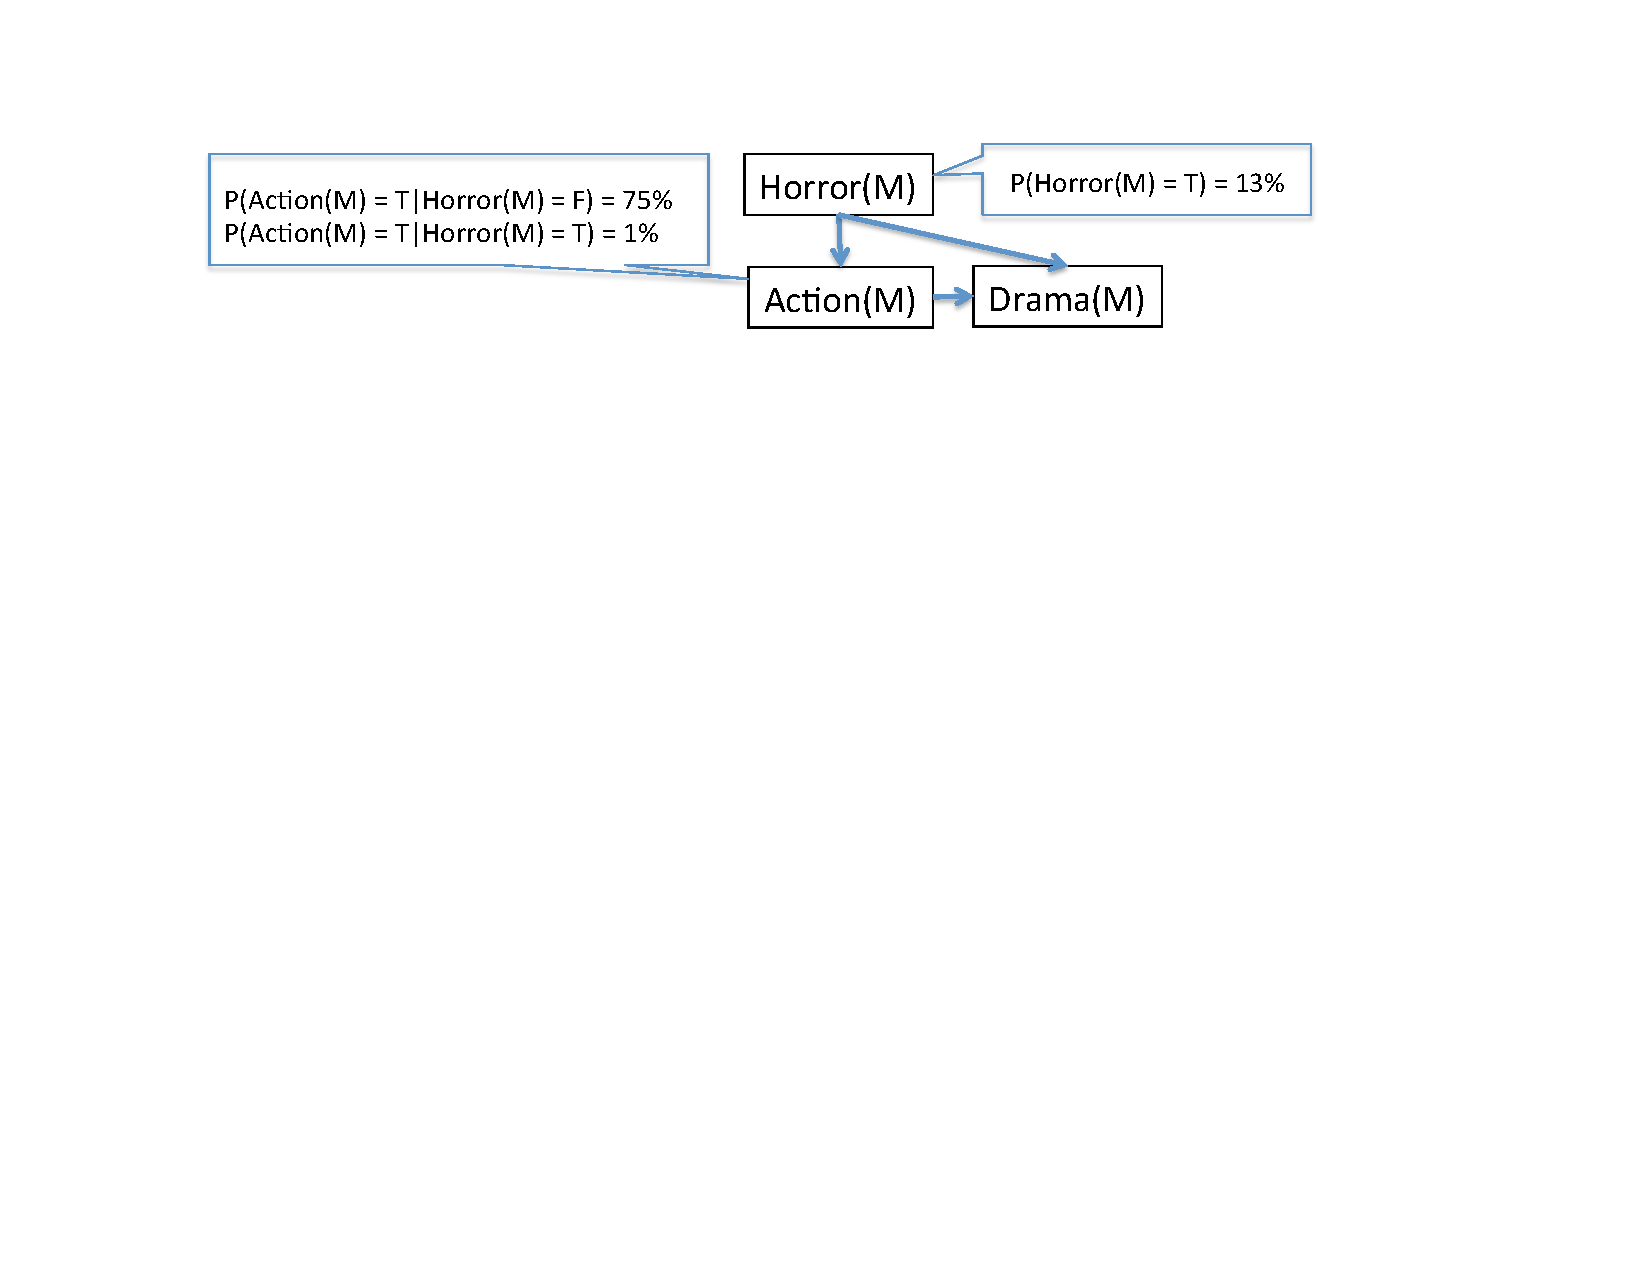
\includegraphics[width=1\textwidth] 
 		{movie-bn2.pdf}
 		\caption[Example of conditional and marginal probabilities computed from a toy Bayesian network structure. ]{The Bayesian network from Figure~\ref{fig:bn-imdb}, where the node names are expanded using the syntax of parametrized random variables.
 			\label{fig:bn-imdb2}
 		}
 	\end{figure}


Figure~\ref{fig:bns} shows a Parametrized Bayesian network for the Premier League domain that is truly relational in that the functors depend on more than one population variable. For example, shot efficiency does not depend on a match only, but also depends on specifying a team. The BN product formula~\eqref{eq:bn} can be applied to any PBN to compute (estimated) frequencies. In the case of a truly relational PBN, as in Figure~\ref{fig:bns}, the PBN can be viewed as representing database frequencies (rather than data table frequencies as in Figure~\ref{fig:bn-imdb2}). Using Getoor's terminology, the PBN can be viewed as a Statistical-Relational Model (SRM)~\cite{Getoor2001a,Schulte2014,Schulte2017a}.


%\footnote{\textbf{Sarah}: add marginal probability P(res=win) for object parameters}
 	\begin{figure}[t]
 		\centering
 		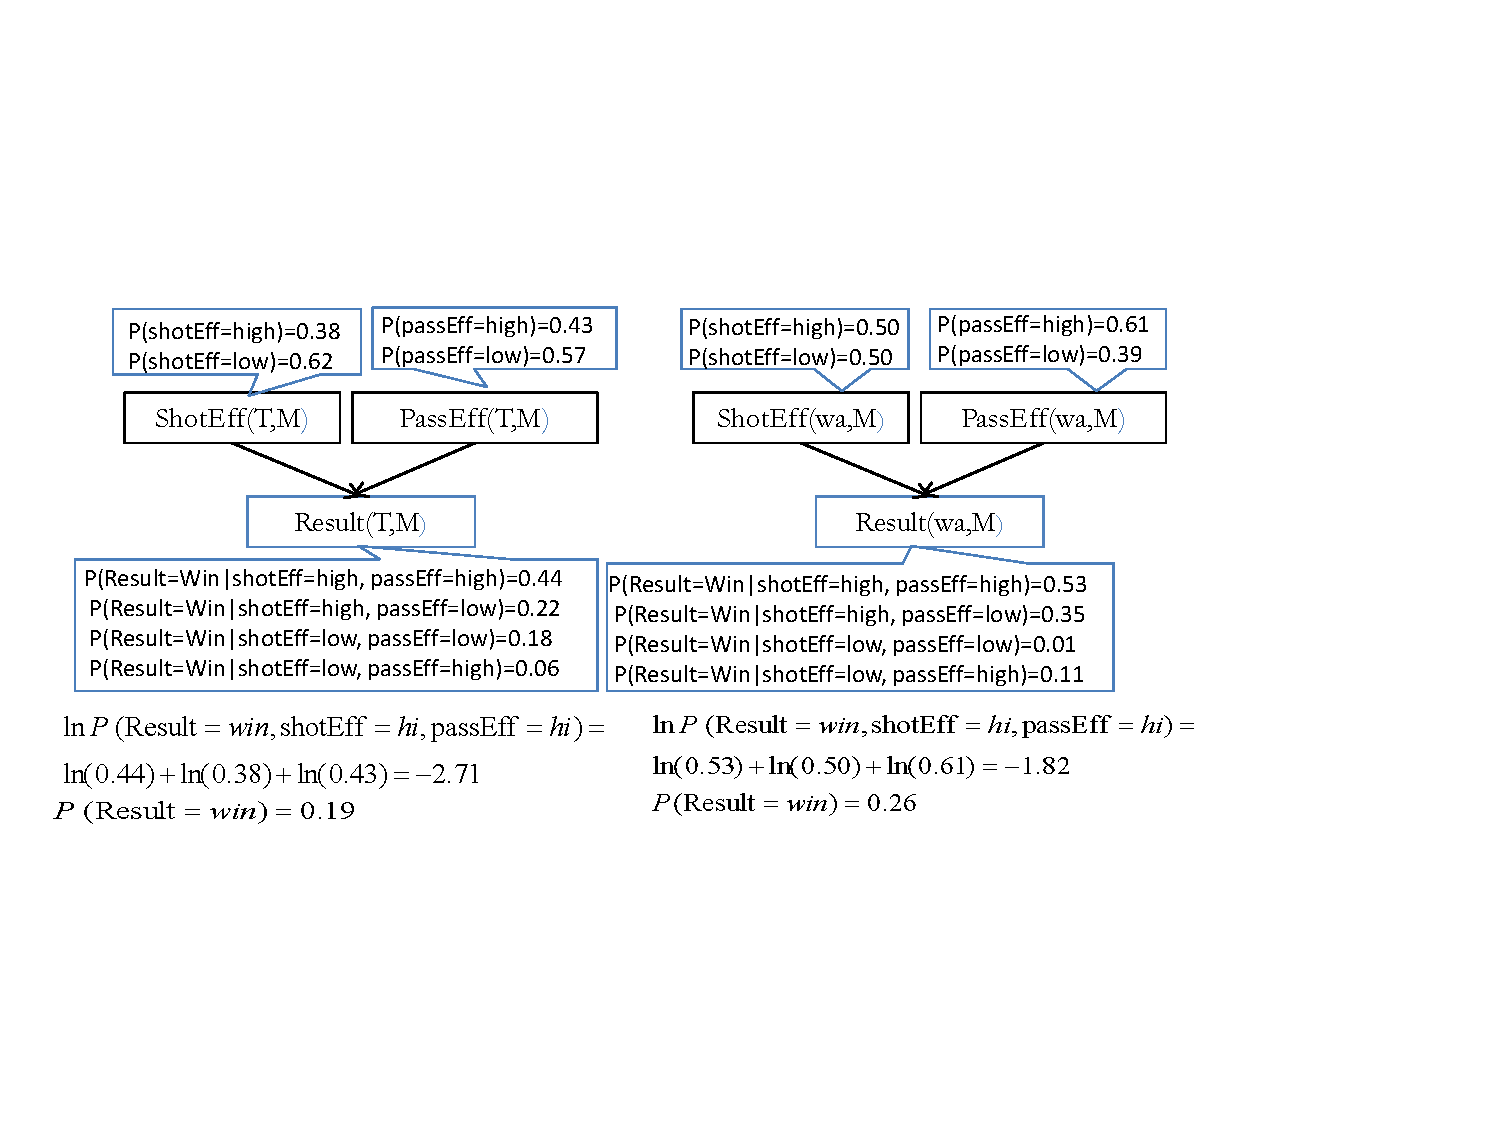
\includegraphics[width=1\textwidth] 
 		{wa.pdf}
 		\caption[Example of joint and marginal probabilities computed from a toy Bayesian network structure. ]{Example of joint and marginal probabilities computed from a toy Bayesian network structure. The parameters were estimated from the  Premier League dataset. (left): A class model Bayesian network $\model_{\class}$ for all teams with class parameters $\parameters_{\class}$. The first-order variable $T$ ranges over teams, and the first-order variable $M$ over matches. For compactness, conditional probabilities omit the first-order variables and constants. (right): The same Bayesian network structure with object parameters $\parameters_{\object}$ learned for Wigan Athletics ($T = WA$). 
 			%We show only the Markov blanket of the Results node to simplify. 
 			\label{fig:bns}
 		}
 	\end{figure}
			

	\subsection{Likelihood Score for Parametrized Bayesian Networks.}\label{sec:log}
	
	A standard method for applying a generative model assumes that the generative model represents normal behavior since it was learned from the entire population. An object is deemed an outlier if the model assigns sufficiently low likelihood to generating its features \cite{Cansado2008}. This likelihood method is an important baseline for our investigation.
	%so we define the likelihood function formally in this section. 
The other outlier scores we consider can be viewed as improved variants of the likelihood approach. 
	Defining a likelihood for relational data is more complicated than for i.i.d. data, because an object is characterized not only by a feature vector, but by an object  database.
	% that lists the object's links and the attributes of linked entities. 
	%For the model likelihood function $\lnlikelihood(\model,\D)$, where $\model$ denotes a Bayesian network, 
	We employ the previously defined normalized relational log-likelihood  score \cite{Schulte2011,Xiang2011}, which can be computed as follows for a given Bayesian network  and database.
	
	%\begin{eqnarray}
	%\lnlikelihood(\model,\D) =   \sum_{i=1}^{n}\sum_{j=1}^{\states_{i}} \sum_{\parents_{i}}\\ P_{\D}(\feature_{i} = \nodevalue_{ij},\parents_{i})\ln \parameter_{\model}(\feature_{i} = \nodevalue_{ij}|\parents_{i})  \nonumber
	%\end{eqnarray}
	
	\begin{equation} \label{eq:likelihood}
		\loglikelihood(\D,\model,\parameters) =   \sum_{i=1}^{n}\sum_{j=1}^{\states_{i}} \sum_{\parents_{i}}\P_{\D}(\nodevalue_{ij},\parents_{i})\ln \parameter(\nodevalue_{ij}|\parents_{i})  
	\end{equation}
	
	
	Equation~\eqref{eq:likelihood} has the same form of the standard BN log-likelihood function for vectorial i.i.d. data~\cite{Campos2006}}, except that parent-child instantiation counts are standardized to be proportions \cite{Schulte2011}. For the notations please refer to Table~\ref{table:notation}. The condition under which the score of Equation~\eqref{eq:likelihood} sums to 1 over all relational datasets are discussed in \cite{Schulte2011}.\footnote{Briefly, if the Parametrized Bayesian Network is viewed as a template for an unrolled ground network, then (1) the ground network cannot contain cycles, and (2) each ground network cannot have multiple parent instantiations; see also \cite{Heckerman+al:SRL07}.}  The equation can be read as follows.
	
	\begin{enumerate}
		\item For each parent-child configuration, 
		use the conditional probability of the child given the parent.
		\item Multiply the logarithm of the conditional probability by the database frequency of the parent-child configuration. 
		%The instantiation proportion is the number of instantiating groundings, divided by the total number of possible instantiations.
		\item Sum this product over all parent-child configurations and all nodes. 
	\end{enumerate}
	
	%\begin{eqnarray}
	%\lnlikelihood&   \sum_{i=1}^{n}\sum_{j=1}^{\states_{i}} \sum_{\parents_{i}} P_{\D}(\feature_{i} = \nodevalue_{ij},\parents_{i})\ln \parameter_{\model}(\feature_{i} = \nodevalue_{ij}|\parents_{i})
	%\end{eqnarray}
	
	The maximum of the relational log-likelihood ~\eqref{eq:likelihood} is given by the empirical database frequencies \cite[Prop.3.1.]{Schulte2011}. In all our experiments we use these maximum likelihood parameter estimates.
	
	{\em Example.} Consider the class-level BN of Figure~\ref{fig:bns}(left). The family configuration \begin{displaymath} \it{passEff(T,M)=high}, shotEff(T,M)=high, Result(T,M)=win\end{displaymath} contributes one term to the log-likelihood score For the population database $\D$, this term is 
\begin{eqnarray*}
P_{D}(\it{passEff(T,M)=high}, shotEff(T,M)=high, Result(T,M)=win) &\times&\\ \ln P(Result(T,M)=win|\it{passEff(T,M)=high}, shotEff(T,M)=high)  &=&\\ 0.1 \times \ln(0.44) =-0.08 & &
\end{eqnarray*}
where the database frequency 0.1 is computed as in Table~\ref{table:counts} and the conditional probability 0.44 is the parameter specified by the Bayesian network of Figure~\ref{fig:bns}. 
	
		
	For the  Wigan Athletics data $\D_{WA}$, the corresponding term is 
	\begin{eqnarray*}
P_{\D_{WA}}(\it{passEff(WA,M)=high}, shotEff(WA,M)=high, Result(WA,M)=win) &\times&\\ \ln P(Result(WA,M)=win|\it{passEff(WA,M)=high}, shotEff(WA,M)=high)  &=&\\ 0.18 \times \ln(0.44) =-0.14 & &
\end{eqnarray*}
where the database frequency 0.18 is computed as in Table~\ref{table:counts} and the conditional probability 0.44 is the parameter specified by the Bayesian network of Figure~\ref{fig:bns}(left). 


\section{Exceptional Model Mining for Relational Data} \label{sec:eld}

This section describes our approach to applying the EMM framework to relational data, using the following notation.
%
%In this section, we introduce a novel model-based outlier score, that extends the relational log-likelihood~\eqref{eq:likelihood}, and outline the steps involved in the score computation.
%\subsection{Computation Flow}  
%We use the following notation to define the computation steps for the relational outlier scores examined in this paper.
\begin{itemize}
	\item $\D_{\Class}$ is the database for the entire class of objects; cf. Table~\ref{table:data}. This database defines the \textbf{class distribution} $P_{\Class} \equiv P_{\D_{\class}}$.
	\item $\D_{\object}$ is the restriction of the input database to the target object; cf. Table~\ref{table:individual}. This database defines the \textbf{object distribution} $P_{\object} \equiv P_{\D_{\object}}$.
	\item $\model_{\Class}$ is a Bayesian network structure learned with $\D_{\Class}$ as the input database. Note that we use the entire population data to learn the Bayesian network structure. Therefore, Bayesian network structure is the same across different individuals.
	\item $\parameters_{\Class}$ resp. $\parameters_{\object}$ are parameters learned for $\model_{\Class}$ using $\D_{\class}$ resp. $\D_{\object}$ as the input database.
\end{itemize}

Figure~\ref{fig:flow} illustrates these concepts and the system flow for computing an outlier score. First, we learn a Bayesian network structure $\model_{\Class}$ for the entire population using a previous learning algorithm (see Section~\ref{sec:methods}). We then compute an {\em outlierness metric} that evaluates how much the object model deviates from the class model. 
%
%\subsection{Definition of Log-Likelihood Distance Outlier Metric} 
%
For a given model type, quantifying the extent to which an object model deviates from the population class model is the main research question in EMM~\cite{Duivesteijn2016}. In this paper we examine several outlierness metrics that are based on the likelihood ratio between the object model and the class model. 
A novel metric that we propose is the \textbf{expected log-likelihood distance} ($\mid$). It is defined as follows for each feature $i$; the total score is the sum of feature-wise scores. Section~\ref{sec:divergence-examples}  provides example computations.


\begin{figure}[htbp]
	\centering
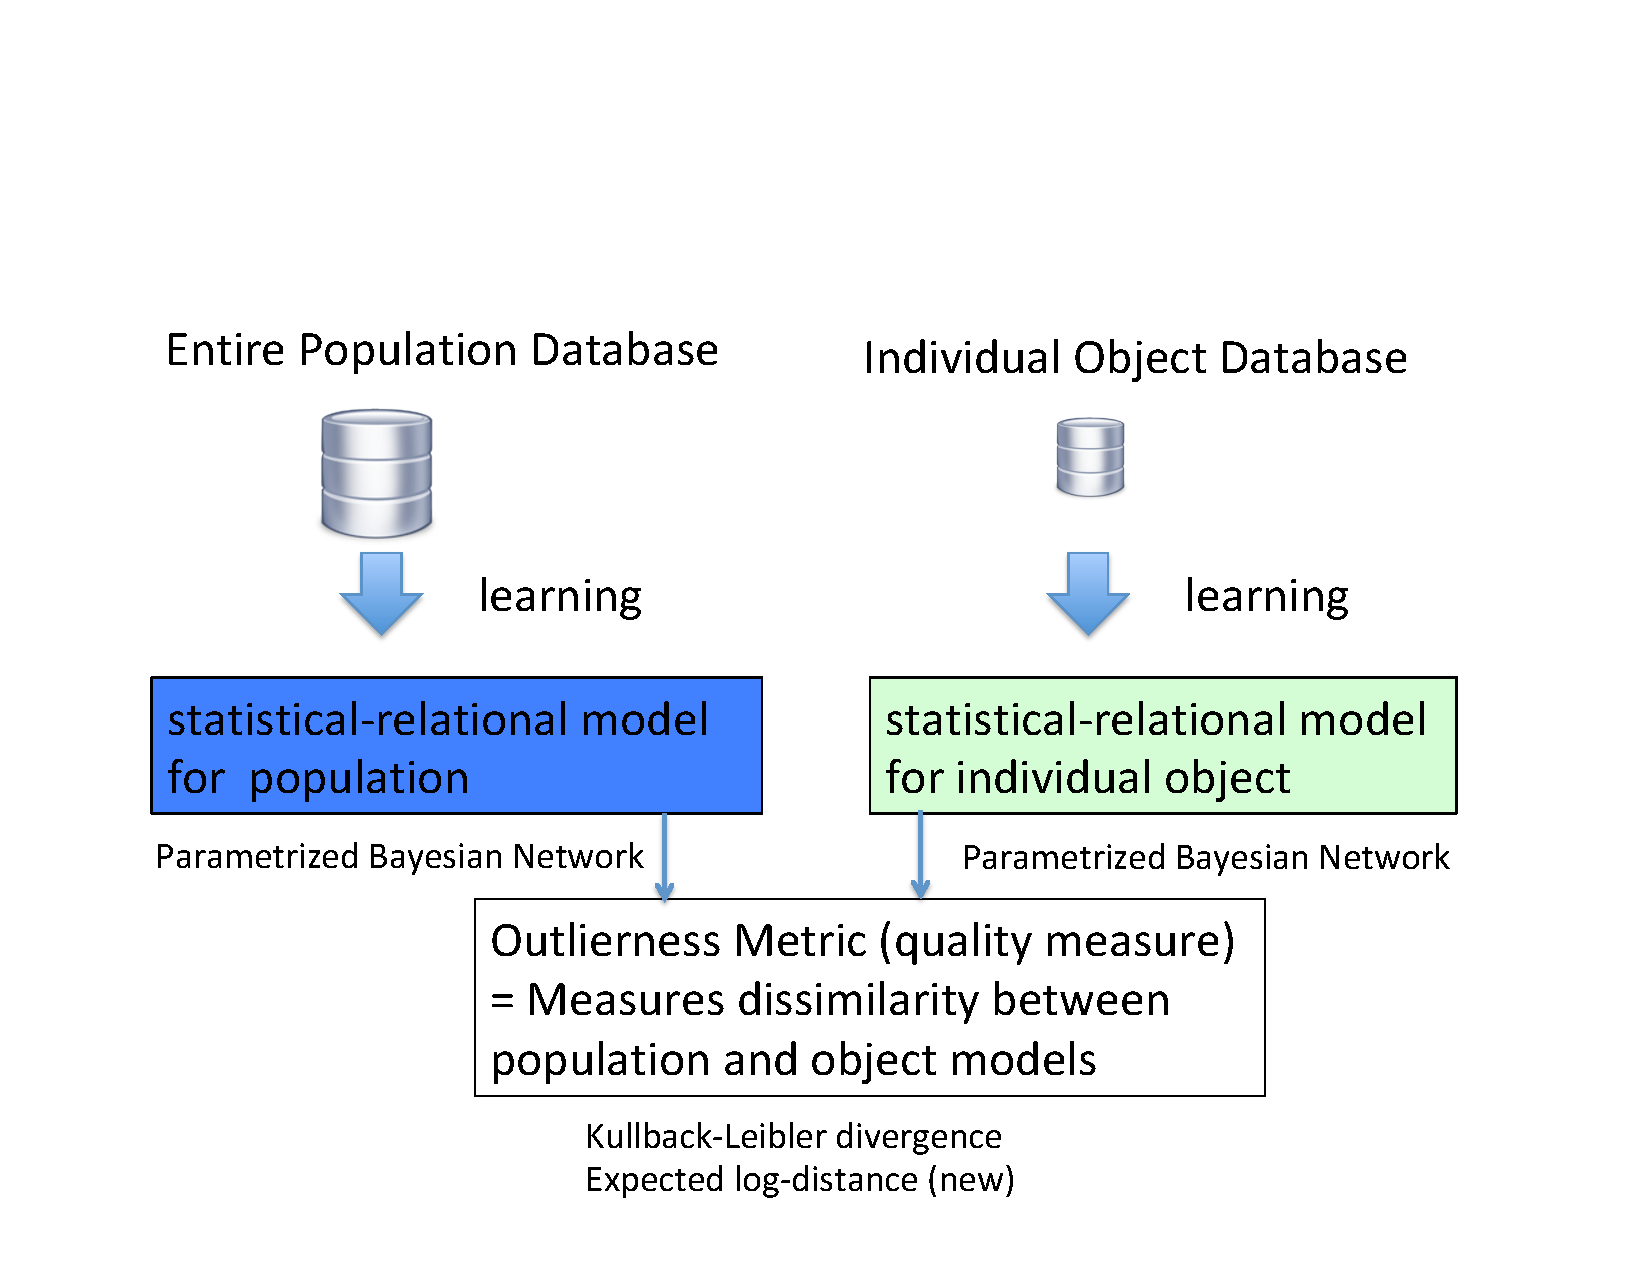
\includegraphics[width=0.8\textwidth]{emm-srl.pdf}
% pdf from SSCI-2015
	\caption{Exceptional Model Mining for statistical-relational models (cf. Figure~\ref{fig:emm}). The model class we utilize in this paper are Parametrized Bayesian networks, with a log-linear likelihood function. As outlierness metrics we consider the standard Kullback-Leibler divergence, and the novel divergence $\mid$ described in the text.
		\label{fig:flow}}
\end{figure}


\begin{eqnarray}
\mid_{i} & = & \sum_{j=1}^{\states_{i}} P_{\object}(\nodevalue_{ij}) \left|\ln \frac{\parameter_{\object}( \nodevalue_{ij})}{\parameter_{\Class}( \nodevalue_{ij})}\right|+ \label{eq:fd}\\
& & \sum_{j=1}^{\states_{i}} \sum_{\parents_{i}} 
P_{\object}( \nodevalue_{ij},\parents_{i})
\left|\ln \frac{\parameter_{\object}( \nodevalue_{ij}|\parents_{i})}{\parameter_{\object}(\nodevalue_{ij})} - \ln \frac{\parameter_{\Class}( \nodevalue_{ij}|\parents_{i})}{\parameter_{\Class}(\nodevalue_{ij})}\right|. \label{eq:mi}
\end{eqnarray}

\subsection{Interpretation}

The first sum~\eqref{eq:fd} is the \textbf{single-feature} component, where each feature is considered independently of all others. It computes the expected log-distance with respect to  the single feature value probabilities between the object and the class models. 
%For example, the single-feature sum for the feature ``Goal" of Van Persie is 5/8. 
%
The second $\mid$ sum~\eqref{eq:mi} is the \textbf{mutual information component}, based on the mutual information among all features. It computes the expected log-distance between the object and the class models with respect to the mutual information of feature value assignments.
%measures the expected distance in 
%%{\em multi-variate mutual information} 
%{\em association component} between the object and the class distributions. 
Intuitively, the first sum measures how the models differ if we treat each feature in isolation. The second sum measures how the models differ in terms of how strongly parent and child features are associated with each other. 


\subsection{Motivation} 

The motivation for the mutual information decomposition is two-fold. 
(1) {\em Interpretability.} This is very important for outlier detection. The single-feature components are easy to interpret since they involve no feature interactions. Each parent-child local factor is based on the average relevance of parent values for predicting the value of the child node, where relevance is measured by $$\ln \frac{\parameter(\nodevalue_{ij}|\parents_{i})}{\parameter(\nodevalue_{ij})}.$$ This relevance term  is basically the same as the widely used lift measure \cite{Tuffery2011}, hence is an intuitively meaningful quantity. The $\mid$ score compares how relevant a given parent condition is in the object data with how relevant it is in the general class. 


(2) {\em Avoiding cancellations.} 
For different child-parent configurations, the different components of the $\mid$ sum may have different signs. This leads to a partial cancelling of differences between the class and object distributions. Since our goal is to assess the distinctness of an object, {\em we do not want differences to cancel out.} Taking distances as in Equations~\eqref{eq:fd} and ~\eqref{eq:mi} avoids the undesirable loss of information. The general point is that averaging differences is appropriate when considering costs, or utilities, but not appropriate for assessing the distinctness of an object. In contrast, the absolute values add differences regardless of their sign. The next section provides comparison scores and example computations that illustrate the cancelling phenomenon that occurs without adding absolute values. The subsequent section uses Taylor series analysis for a theoretical understanding of the cancelling phenomenon: We show that without the absolute values (as with $\lr$), the first-order term in the Taylor series approximation vanishes, whereas with the absolute values (as with $\eld$), the first-order term is equivalent to the total variation distance (L1 norm). 

\section{Comparison Scores} \label{sec:metrics}

We introduce several alternative likelihood-ratio based outlier scores, following a lesion design where different scores omit different components of our main $\mid$ proposal. %We introduce the scores. 
To illustrate their essential difference with $\mid$, we give toy examples before we evaluate them on full datasets.

\subsection{Definition of Comparison Outlier Scores}

\paragraph{Log-likelihood Ratio Score.} Our first comparison score omits the absolute values from the $\mid$ score: 

\begin{eqnarray*}
\lr_{i} & = & \sum_{j=1}^{\states_{i}} P_{\object}(\nodevalue_{ij}) \ln \frac{\parameter_{\object}( \nodevalue_{ij})}{\parameter_{\Class}( \nodevalue_{ij})}+ \sum_{j=1}^{\states_{i}} \sum_{\parents_{i}} 
P_{\object}( \nodevalue_{ij},\parents_{i})
(\ln \frac{\parameter_{\object}( \nodevalue_{ij}|\parents_{i})}{\parameter_{\object}(\nodevalue_{ij})} - \ln \frac{\parameter_{\Class}( \nodevalue_{ij}|\parents_{i})}{\parameter_{\Class}(\nodevalue_{ij})}).
\end{eqnarray*}

By using the \textbf{mutual information decomposition:}


\begin{equation} \label{eq:decompose}
\ln \frac{\parameter_{\object}( \nodevalue_{ij}|\parents_{i})}{\parameter_{\Class}( \nodevalue_{ij}|\parents_{i})} = \ln \frac{\parameter_{\object}(\nodevalue_{ij}|\parents_{i})}{\parameter_{\object}(\nodevalue_{ij})} - \ln \frac{\parameter_{\Class}( \nodevalue_{ij}|\parents_{i})}{\parameter_{\Class}(\nodevalue_{ij})} + \ln \frac{\parameter_{\object}( \nodevalue_{ij})}{\parameter_{\Class}( \nodevalue_{ij})},
\end{equation}

\noindent it can be shown that the $\mid$ score without the absolute values is equivalent to 
the likelihood ratio, or {\bf log-likelihood difference}:
%. The log-likelihood difference is defined by

\begin{equation} \label{eq:log-diff}
\lr(\D_{\object},\model_{\Class},\parameters_{\object}) \equiv \loglikelihood(\D_{\object},\model_{\Class},\parameters_{\object}) - \loglikelihood(\D_{\object},\model_{\Class},\parameters_{\Class}).
\end{equation}

Assuming maximum likelihood parameter estimation, $\lr$ is equivalent to the Kullback-Leibler divergence between the class-level and object-level parameters~\cite{Campos2006}. The log-likelihood difference compares  how well the class-level parameters fit the object data with respect to a particular object, vs. how well the object parameters fit the object data. In terms of the conditional probability parameters, it measures how much the log-conditional probabilities in the class distribution differ from those in the object distribution. 
%Note that this definition applies only for relational data where an individual is characterized by a substructure rather than a ``flat'' feature vector. 
%
\paragraph{The Feature Divergence Score.}
The feature divergence outlier score $\fd$ uses only part~\eqref{eq:fd} of the $\mid$ score. That is, it considers each feature independent of all others.  $\fd$ computes the expected log-distance with respect to  the single feature value probabilities between the object and the class models. This can be computed using the following formula:
\begin{equation}
\fd_{i}	=\sum_{i=1}^{n}\sum_{j=1}^{\states_{i}} P_{\object}( \nodevalue_{ij}) \left|\ln \frac{\parameter_{\object}( \nodevalue_{ij})}{\parameter_{\Class}( \nodevalue_{ij})}\right|
\end{equation}


\paragraph{Log-Likelihood Score.} 

In previous work on applying Bayesian networks to outlier detection for i.i.d. (independent and identically-distributed) non-relational data, the outlier metric used was the log-likelihood of a data point \cite{Cansado2008}. This means that an object was deemed an outlier if the model assigns sufficiently low likelihood to generating its features. For relational data, we use the relational log-likelihood \eqref{eq:likelihood} of the target {\em database}:

\begin{equation} \label{eq:loglikelihood-score}
\loglikelihood(\D_{\object},\model_{\Class},\parameters_{\Class}) =   \sum_{i=1}^{n}\sum_{j=1}^{\states_{i}} \sum_{\parents_{i}}\P_{\D}(\nodevalue_{ij},\parents_{i})\ln \parameter(\nodevalue_{ij}|\parents_{i}).
\end{equation}




\subsection{Score Computation Examples} \label{sec:divergence-examples} 
			
			
			We provide three simple examples with only two variables/features that illustrate the computation of the outlier scores. They are designed so that outliers and normal objects are easy to distinguish, and so that it is easy to trace the behavior of an outlier score.
			%The examples also illustrate the concepts of attribute and correlation outlier. 
			The examples therefore serve as thought experiments that bring out the strengths and weaknesses of model-based outlier scores. 
			Figure~\ref{fig:synthetic-bns} describes the BN representation of the examples. For intuition, we can think of a soccer setting, where each match assigns a value to each attribute $F_{1}$ and $F_{2}$ for each player. 
			
			\begin{figure*}[htbp]
				\centering
				\resizebox{1\textwidth}{!}{
					\includegraphics%[width=0.3\textwidth] 
					{DistributionBN-bk-aug17.pdf}
				}
				\caption{Illustrative Bayesian networks with two nodes. The networks are not learned from data, but hand-constructed to be plausible for the soccer domain. (a) {\em High Correlation:} Normal individuals exhibit a strong association between their features, outliers no association. Both normals and outliers have a close to uniform distribution over single features.
					% The outlier distribution misses a correlation that is present in the normal population. The single feature distributions are uniform in both distributions. 
				(b) {\em Low Correlation:} Normal individuals exhibit no association between their features, outliers have a strong association. Both normals and outliers have a close to uniform distribution over single features.
					% The outlier object exhibits a correlation that is not present in the normal population. The single attribute distributions are uniform in both distributions.
				(c) {\em Single Attributes:} Both normal and outlier individuals exhibit a strong association between their features. In normals, 90\% of the time, feature 1 has value 1. For outliers, feature 1 has value 1 only 10\% of the time. 
					%Correlations are the same, but the single feature distributions are not.
					\label{fig:synthetic-bns}}
			\end{figure*}
			
			

%\paragraph{Example Computations.} 
%\footnote{\textbf{Sarah}:caption sizes are funny}


\begin{table}[hbpt]
	\caption{Example computation of different outlier scores for outliers given the distributions of Figure~\ref{fig:synthetic-bns}(a),(b). Negative terms are highlighted by boxes; part of their impact cancels out with positive terms. Our new $\eld$ metric contains no negative terms due to the use of absolute values.
	\label{table:example}}
	
	%\captionsetup[table]{skip=10pt}
	
	\centering
	\resizebox{1\textwidth}{!}{
		\begin{tabular}{|c|p{3cm}|p{6cm}|l|}
			\hline
			Score&$F1=1$ Computation&$F2|F1=1$ Computation&Result\\ \hline
			$\lr$&\begin{tabular}{p{5cm}} $1/2 \ln(0.5/0.5)=0 $\end{tabular}&$1/4\ln(0.5/0.9)+ 1/4\ln(0.5/0.1)$&0.36\\ \hline
			%$ELD$&$1/2|\ln(0.5/0.5)|=0$&$1/4|\ln(0.5/0.9)|+1/4|\ln(0.5/0.1)|$&0.79\\ \hline
		%	$|\lr|$&$0$ (no parents)&\begin{tabular}{p{5cm}}$1/4 |\ln(0.5/0.9)|+1/4|\ln(0.5/0.1)|$\end{tabular}&0.79\\ \hline
			$\fd$&$|\ln(0.5/0.5)|=0$&\begin{tabular}{p{5.5cm}}$1/2|\ln(0.5/0.5)| + 1/2|\ln(0.5/0.5)|$\end{tabular}&0\\ \hline
			%$$\mid$$&$0+0$&$0.79+0$&0.79
			$\mid$&$0$ (no parents)&\begin{tabular}{p{5cm}}$1/2|\ln(0.5/0.5)| + 1/2|\ln(0.5/0.5)| + 
1/4 |\ln(0.5/0.5)-\ln(0.9/0.5)|+1/4 |\ln(0.5/0.5)-\ln(0.1/0.5)|$\end{tabular}&0.79
			
			%$1/4(|\ln(0.9/0.5)-\ln(0.5/0.5)|+|\ln(0.1/0.5)-\ln(0.5/0.5)|+2|\ln(0.5/0.5)|)=0.54$
			\\ \hline
		\end{tabular}}
		%\centering
		\resizebox{1\textwidth}{!}{
			\begin{tabular}{p{11cm}}
				Table 5(a): High Correlation Case. Figure~\ref{fig:synthetic-bns}(a).
				%: The scores for the object and class BNs of Figure~\ref{fig:synthetic-bns}(a).
				
			\end{tabular}}
			
			%
			\centering
			\resizebox{1\textwidth}{!}{
				\begin{tabular}{|l|p{3cm}|p{6cm}|l|}
					\hline
					Score&$F1=1$ Computation&$F2|F1=1$ Computation&Result\\ \hline
					$\lr$&$1/2\ln(0.5/0.5)=0$&$0.5 \cdot 0.9 \ln(0.9/0.5)+ 0.5 \cdot 0.1 \ln(0.1/0.5)$&0.26\\ \hline
					%$ELD$&$1/2|\ln(0.5/0.5)=0|$&$0.5 \cdot 0.9|\ln(0.9/0.5)|+0.5 \cdot 0.1|\ln(0.1/0.5)|$&0.50\\ \hline
					%$|\lr|$&$0$ (no parents) &$0.5 \cdot 0.9 |\ln(0.9/0.5)|+ 0.5 \cdot 0.1 |\ln(0.1/0.5)| $&0.50\\ \hline
					$\fd$&$|\ln(0.5/0.5)|=0$&$1/2|\ln(0.5/0.5)| + 1/2|\ln(0.5/0.5)|$&0\\ \hline
					%$\mid$&$0+0$&$0.5+0$&0.5\\ \hline
						$\mid$&$0$ (no parents) &\begin{tabular}{p{5.5cm}}$1/2|\ln(0.5/0.5)| +1/2|\ln(0.5/0.5)| + 0.5 \cdot 0.9 |\ln(0.9/0.5)-\ln(0.5/0.5)|+ 0.5 \cdot 0.1 |\ln(0.1/0.5)-\ln(0.5/0.5)|
						$\end{tabular}&0.50\\ \hline
				\end{tabular}}
				\resizebox{1\textwidth}{!}{
					\begin{tabular}{p{11cm}}
						Table 5(b): Low Correlation Case. Figure~\ref{fig:synthetic-bns}(b).
						%The scores for the object and class BNs of Figure~\ref{fig:synthetic-bns}(b). 
						
					\end{tabular}}
				\end{table}
				
			

%\subsection{Comparison on Examples}


%
%The single feature distributions are uniform, so the feature component~\eqref{eq:fd} 
%is 0 for each node in both examples.
% 
Table~\ref{table:example} illustrates the computation of the scores. Scores for the $F_{2}$ feature are computed conditional on $F_{1} = 1$. Expectation terms are computed first for $F_{2} = 1$, then $F_{2} = 0$.
The table shows the %undesirable 
cancelling effects in $\lr$. In the high correlation scenario~\ref{fig:synthetic-bns}(a), the outlier object has a lower probability than the normal class distribution of $\it{Match\_Result} = 0$ given that $\it{Shot\_Efficiency} = 1$. Specifically, 0.5 vs. 0.9. The outlier object exhibits a higher probability $\it{Match\_Result} = 1$ than the normal class distribution, conditional on $\it{Shot\_Efficiency} = 1$; specifically, 0.5 vs. 0.1. In line 1, column 2 of Table~\ref{table:example}  the log-ratios $\ln(0.5/0.9)$ and $\ln(0.5/0.1)$ therefore have different signs. In the low correlation scenario~\ref{fig:synthetic-bns}(b), the cancelling occurs in the same way, but with the normal and outlier probabilities reversed. 
The cancelling effect is even stronger for attributes with more than two possible values.

While log-likelihood $\loglikelihood$ is a good baseline score for detecting outliers, it fails to detect some clear outliers, as shown in Figure~\ref{fig:logfails}. In that example the strength of the correlation among the attributes is the same in both normal and outlier examples and the only difference is in their feature distributions.

		\begin{figure*}[htbp]
			\centering
			\resizebox{0.9\textwidth}{!}{
				\includegraphics%[width=0.3\textwidth] 
				{logfails.pdf}
			}
			\caption{An example of normal and outlier individuals and their conditional probability tables created using Bayesian network shown in Figure~\ref{fig:synthetic-bns}(c). Log-likelihood assigns the same score to the normal and individuals in this example, while $\it{FD}$ is able to differentiate between these two individuals.
				%Correlations are the same, but the single feature distributions are not.
				\label{fig:logfails}}
		\end{figure*}
		



%\subsection{Visualization}\label{sec:visual}
%	
%We generated three synthetic datasets with normal and outlier players using the distributions represented in the three Bayesian networks of Figure~\ref{fig:synthetic-bns}. The main goal of designing synthetic experiments is to test the methods on  easy to detect outliers. We provide a 1D scatter plot for each outlier method to visualize the scores assigned to each player. We used the $\it{mlbench}$ package in $\it{R}$ to generate synthetic features in matches, following these distributions for 240 normal players and 40 outliers. (There were 280 players in our Premier League dataset.) Each player participates in 38 matches, similar to the real-world data. Each match assigns a value to each feature $F_i, i =  1,2$ for each player. This design yields the following three synthetic datasets. 
%				\begin{description}
%					\item\textbf{High Correlation} See Figure~\ref{fig:synthetic-bns}(a).
%					\item\textbf{Low Correlation} See Figure~\ref{fig:synthetic-bns}(b).
%					\item\textbf{Single features} See Figure~\ref{fig:synthetic-bns}(c).
%				\end{description}
%				
%Figure~\ref{fig:1DPlots} provides scatter plots for each synthetic dataset and each comparison outlier metric. The figure is best viewed on screen. As entailed by Proposition~\ref{prop:divergence}(Part \ref{clause:inequalities}), the $\mid$ metric maps players to the largest range of outlier scores. It also provides the best separation of normal from abnormal players: The normal players receive low anomaly scores and hence are clustered to the left of the $\mid$ scatter plot, whereas the abnormal players receive high scores and hence are clustered on the right. The $|\lr|$ metric  also shows a larger range of scores and a better discrimination compared to the $\lr$ metric. This illustrates the value of using distances rather than differences. In Section~\ref{sec:detection} we provide an aggregate detection accuracy score that quantifies this values.
%

%
%	\begin{figure}
%		\centering     %%% not \center
%		\subfigure[Distribution of different outlier scores in Synthetic Dataset- Single Feature. ]{\label{fig:Feature}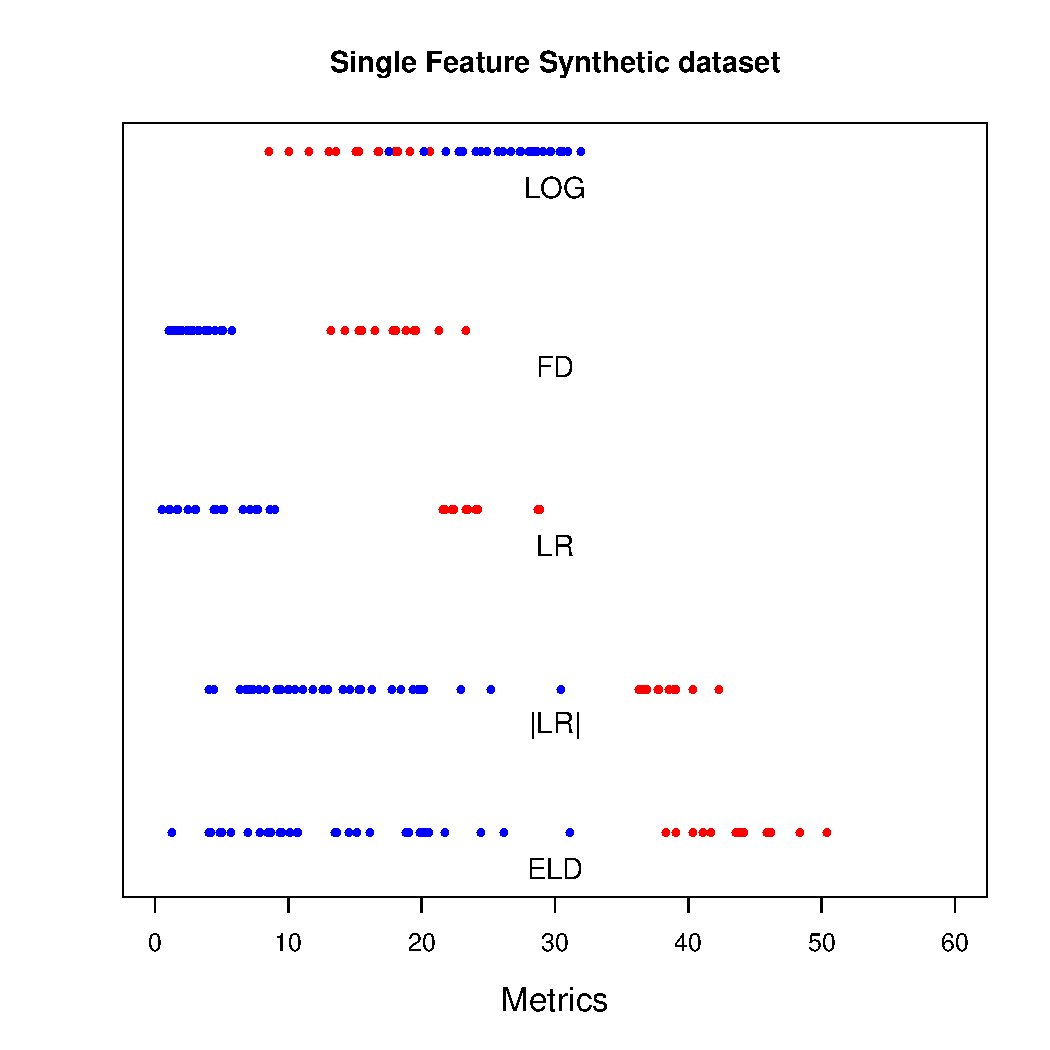
\includegraphics[width=0.48\textwidth]{DistributionPlots/sumFeature-bk-feb2016.pdf}}
%		\subfigure[Distribution of different outlier scores in Synthetic Dataset- Low correlation]{\label{fig:LowCor}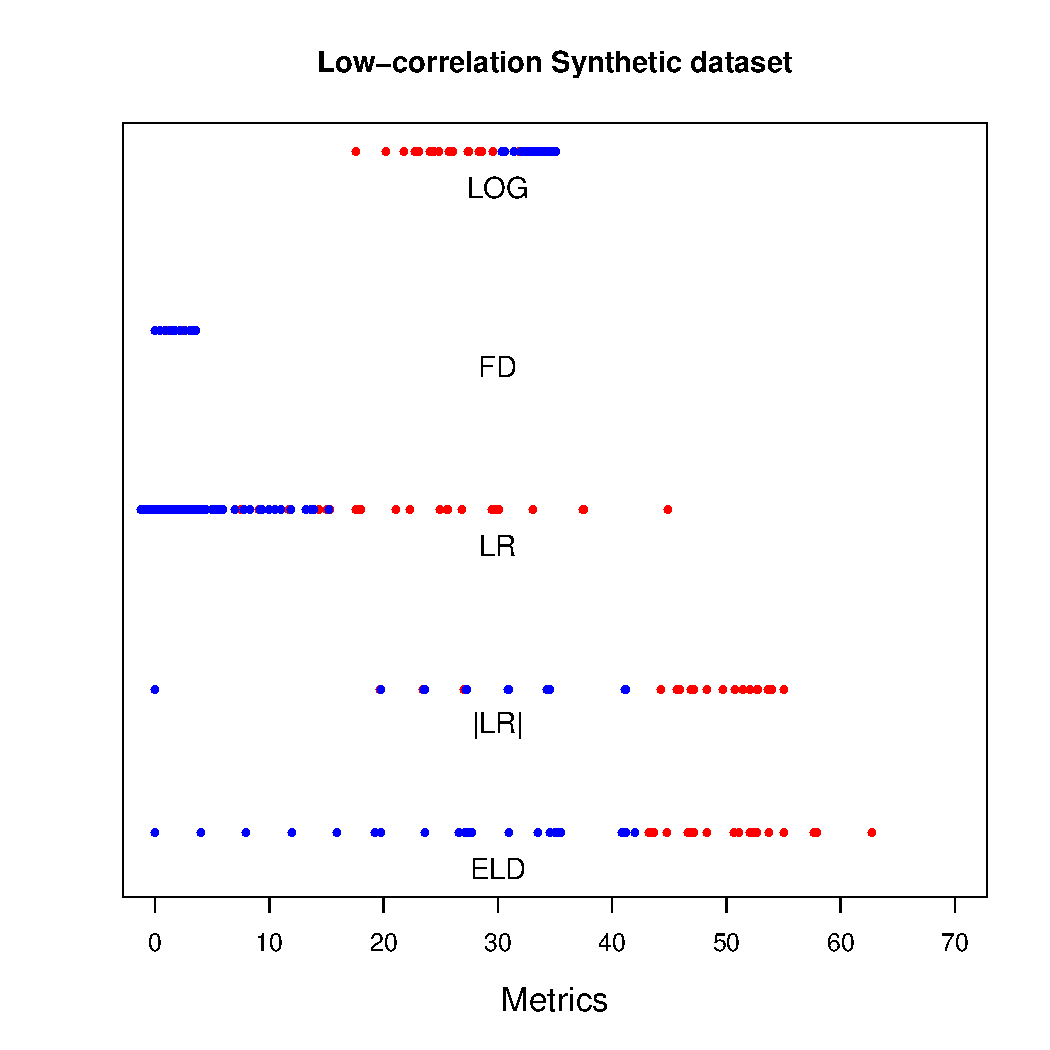
\includegraphics[width=0.5\textwidth]{DistributionPlots/sumSep-bk-feb2016.pdf}}
%		\subfigure[Distribution of different outlier scores in Synthetic Dataset- High correlation]{\label{fig:HighCor}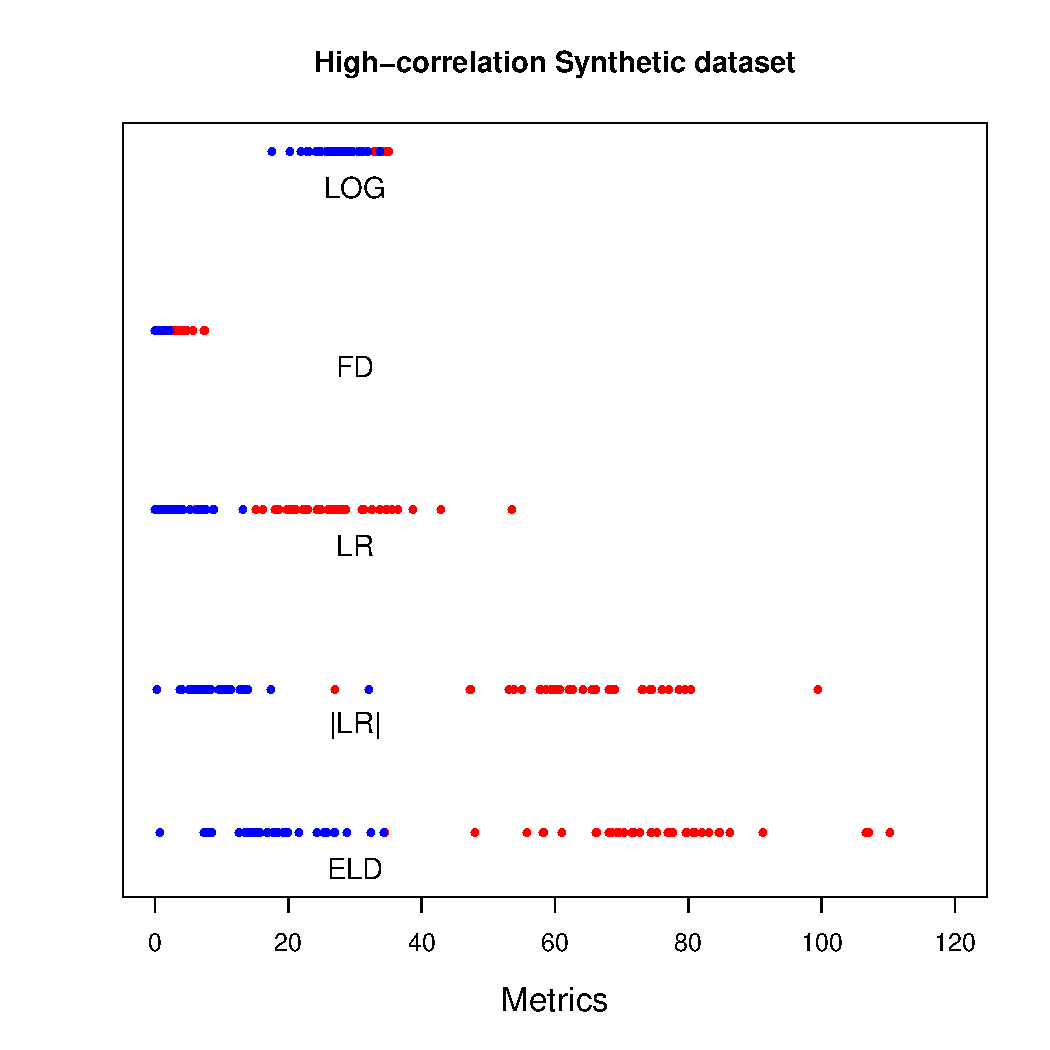
\includegraphics[width=0.5\textwidth]{DistributionPlots/sumSV-bk-feb2016.pdf}}
%		\caption{Visualizing likelihood-based outlier metrics on our three synthetic datasets. The figure is best viewed on the screen. Score values are shown on the $x$-axis; higher values should indicate more anomalous players. For each dataset and each metric, we provide a 1D scatterplot of the 280 synthetic player scores. In the scatterplot, blue dots represent normal players, and red dots represent anomalous players.}\label{fig:1DPlots}
%	\end{figure}
%\section{Feature Divergence Object Outlier Score}\label{sec:fd}

\begin{figure*}[htbp]
	\centering
	\resizebox{0.9\textwidth}{!}{
		\includegraphics%[width=0.3\textwidth] 
		{fdfails.pdf}
	}
	\caption{An example of normal and outlier individuals and  their conditional probability tables  created using Bayesian network shown in Figure~\ref{fig:synthetic-bns}(a). FD assigns the same score to the normal and individuals in this example, while $\it{LR}$ is able to differentiate between these two individuals.
		%Correlations are the same, but the single feature distributions are not.
		\label{fig:fdfails}}
\end{figure*}
Conversely, if there is a correlation among the attributes of individuals, the feature divergence score $\fd$ fails to take it into account and therefore fails to differentiate between normal and outlier individuals. Figure~\ref{fig:fdfails} shows an example where the normal individual has a correlation among its attributes while the outlier object does not have a correlation. The $\textit{FD}$ metric cannot separate  those two individuals.

\section{Theoretical Analysis and Comparison}
%\todo{introduce $|LR|$ as well?}
The mathematical analysis of this section relates the $KLD$ and $\mid$ divergences defined in the above sections to other well-known scores. Readers who wish to proceed to empirical evaluation can omit this section without loss of generality. A well-known Taylor series argument shows that KLD can be approximated by Pearson's $\chi^{2}$ statistic \cite{Nielsen2014}. We use a similar Taylor series approximation to show that our ELD divergence can be approximated by the total variation distance (TVD), also known as the L1-norm, whose statistical properties are well understood~\cite{Beirlant2001,Beirlant1994}. 
%The Taylor series approximation provides a clear explanation of the cancellation phenomenon: For KLD and $\chi^{2}$, the first-order term in the Taylor series vanishes, whereas for ELD and TVD it does not. 
Our analysis uses the $f$-divergence framework, which unifies all the standard divergence definitions for probability distributions. The $f$-divergence analysis shows the generality of the cancellation phenomenon: the first-order Taylor series term vanishes for all $f$-divergences whose generator $f$ is differentiable at $\lambda = 1$, which includes all standard $f$-divergences (including KLD), except for those that use absolute values. 

\paragraph{The $\chi^2$ approximation for $f$-divergences.}
To focus the mathematics on the essential insights, we discuss the case of divergences defined a single discrete random variable $\feature$ with possible values $\nodevalue_{1},\ldots,\nodevalue_{m}$. The results carry over to the joint BN distributions over discrete variables considered in this paper, by applying the approximation to each parent state. Given two probability distributions $P_{1}$ and $P_{2}$ over the values of $\feature$, an $f$-divergence is of the form 

\begin{equation}
\label{eq:f-divergence}
I_{f}(P_{1}||P_{2}) \equiv \sum_{i=1}^{m} P_{1}(\nodevalue_{1}) f\left(\frac{P_{2}(\nodevalue_{i})}{P_{1}(\nodevalue_{i})}\right)
\end{equation}

where the \textbf{generator} $f:R \rightarrow R$ is a convex function such that $f(1)=0$. 
The generator transforms the ratio of the two compared probabilities for each possible value; the $f$-divergence is the weighted average of the transformed ratios. Common divergences can be represented by choosing a suitable generator. For example, KLD is generated by $f(u) = -\ln(u)$, the $\chi^{2}$ statistic by $f(u) = (1-u)^{2}/u$, and the TVD by $f(u) = |u-1|$ \cite{Nielsen2014}. 

An $f$-divergence $I_{f}$ can be approximated by  by replacing $f$ with its Taylor series expansion around the point $u=1$. Assuming that the derivatives $f^{(i)(1)}$ of any order exist, the Taylor series for $f$ takes the form $f(u) = \sum_{i=0}^{\infty} f^{(i)}(1)/i! [u-1]^{i},$ where the $i=0$ term is 0 because $f(1) = 0$. If the generator $f$ is twice differentiabe, the first-order term with $i=1$ vanishes, and the remaining second-order term with $i=2$ is a scaled $\chi^{2}$ statistic \cite{Nielsen2014}:

\begin{proposition}[Nielsen and Nock 2014] \label{prop:xi-square}
Assume that the generator $f$ for $I_{f}$ is twice differentiable.   

\begin{enumerate}
\item The $i=1$ Taylor series term for  $I_{f}$ around $u=1$ is 0.
\item The $i=2$ Taylor series term for  $I_{f}$ around $u=1$ is a scaled $\chi^{2}$ divergence.
\end{enumerate}


Therefore the second-order Taylor series approximation to $I_{f}$ is scaled $\chi^{2}$-divergence:

$$I_{f}(P_{1}||P_{2}) \approx \frac{f''(1)}{2} \chi^{2}(P_{1}||P_{2}) = \frac{f''(1)}{2} 
\sum_{i=1}^{m}  \frac{(P_{2}(\nodevalue_{i})-P_{1}(\nodevalue_{i}))^{2}}
 {P_{1}(\nodevalue_{i})}.$$ 
\end{proposition} 
{\em Proof Outline.} 
The first-order term reduces to $f'(1) [\sum_{i=1}^{m} P_{2}(\nodevalue_{i}) - \sum_{i=1}^{m} P_{1}(\nodevalue_{i})]$, which vanishes because both probability measures sum to 1. The second-order term reduces to $ \frac{f''(1)}{2} \chi^{2}(P_{1}||P_{2})$. The details are given in the Appendix~\ref{sec:proofs}. 

\paragraph{The TVD approximation for $\eld$.}

Our ELD metric is an example of transforming an $f$-divergence with absolute values by replacing the generator $f$ with $|f|$; in our case, replacing $-\ln(u)$ by $|-ln(u)|$ (cf. Equation~\eqref{eq:log-diff}). Because $|x|$ is not differentiable at 0,  the absolute value generator $|f|$ is generally not differentiable at $u=1$, so Proposition~\ref{prop:xi-square} does not apply. To apply the Taylor series analysis, we can rewrite the absolute value divergence as a positive sum where $f(u)>0$ and a negative sum where $f(u) < 0$. 

\begin{equation*} \label{eq:f-absolute}
I_{|f|}(P_{1}||P_{2}) \equiv \sum_{i:f(\frac{P_{2}(\nodevalue_{i})}{P_{1}(\nodevalue_{i})})>0} P_{1}(\nodevalue_{1}) f\left(\frac{P_{2}(\nodevalue_{i})}{P_{1}(\nodevalue_{i})}\right) - \sum_{i:f(\frac{P_{2}(\nodevalue_{i})}{P_{1}(\nodevalue_{i})})<0} P_{1}(\nodevalue_{1}) f\left(\frac{P_{2}(\nodevalue_{i})}{P_{1}(\nodevalue_{i})}\right)
\end{equation*}

In the Taylor series approximation for $\mid$ (using $f=-\ln(u)$ in Equation~\eqref{eq:f-absolute}), cancellation is avoided, so the first-order term does {\em not} vanish, and is in fact equivalent to the Total Variation Distance:

\begin{proposition} The $i=1$ term in the Taylor series approximation for  $\mid$ around $u=1$ is total variation distance. Therefore 
the first-order Taylor series approximation for $\mid$ is total variation distance:
$$\mid(P_{1}||P_{2}) \approx  \TVD =  \sum_{i} |P_{2}(\nodevalue_{i})-P_{1}(\nodevalue_{i})|$$
\end{proposition}




%
%				\begin{figure}
%				\caption{Visualizing likelihood-based outlier metrics on our three synthetic datasets. Score values are shown on the $x$-axis; higher values should indicate more anomalous players. For each dataset and each metric, we provide a 1D scatterplot of the 280 synthetic player scores. In the scatterplot, empty circles represent normal players, and stars represent anomalous players.}
%				\label{fig:1d}
%									\centering
%									\begin{minipage}{0.45\linewidth}
%										\centering
%										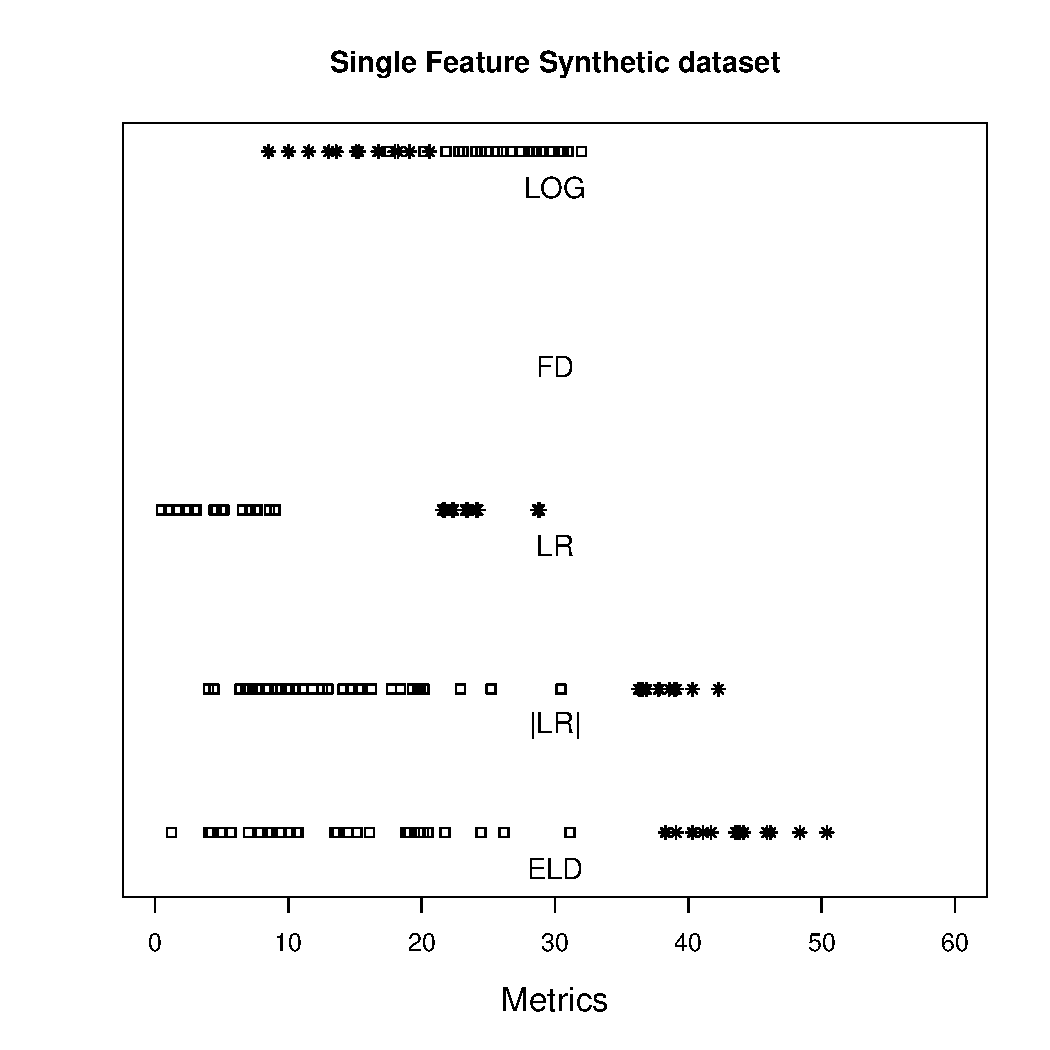
\includegraphics[width=2.5in]{DistributionPlots/sumFeature-bk.pdf}
%										\caption{Distribution of different outlier scores in Synthetic Dataset- Single Feature. \textbf{what happened to FD?}}
%										\label{fig:StrikerSalary}
%									\end{minipage}
%									\hspace{0.05\linewidth}
%									\begin{minipage}{0.45\linewidth}
%										\centering
%										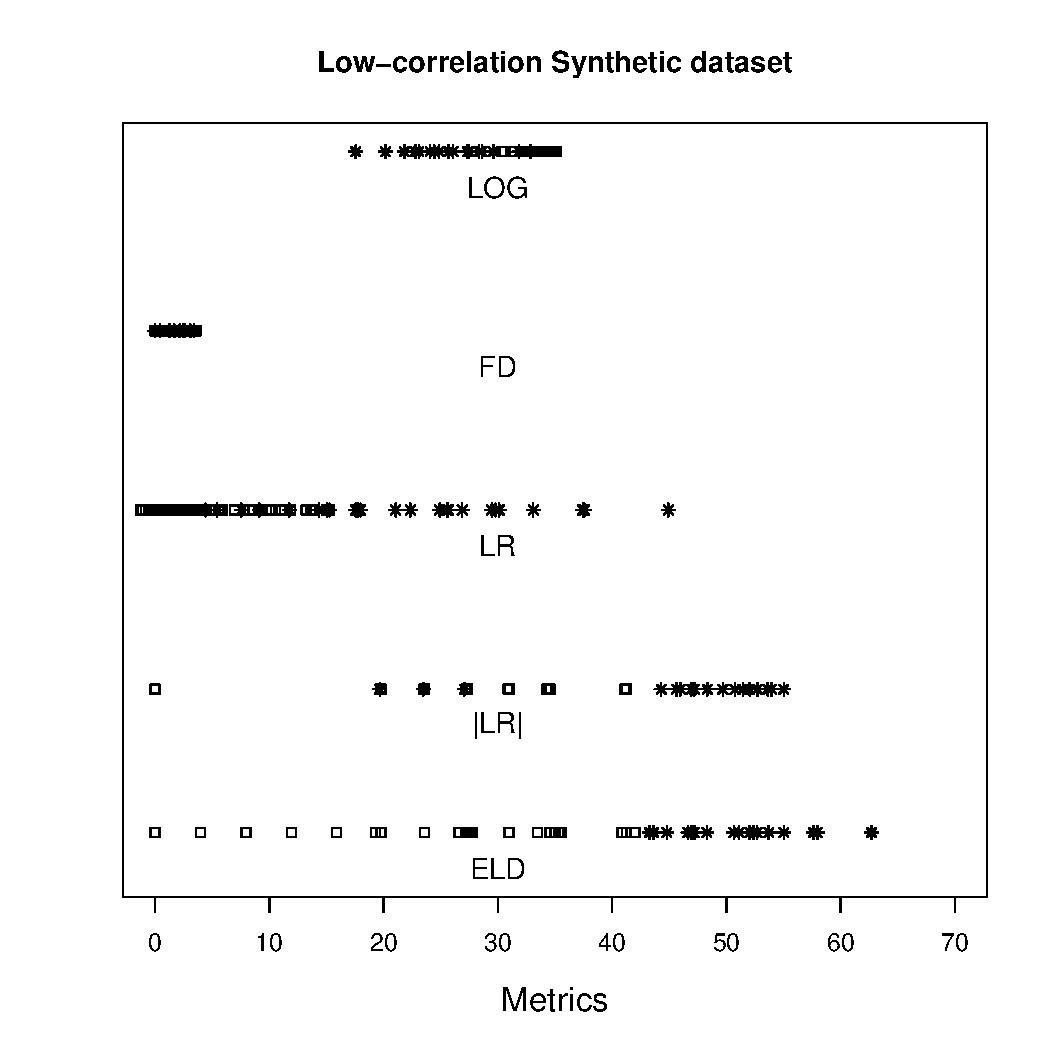
\includegraphics[width=2.5in]{DistributionPlots/sumSep-bk.pdf}
%										\caption{Distribution of different outlier scores in Synthetic Dataset- Low correlation}
%										\label{fig:StrikerShot}
%									\end{minipage}
%									\hspace{0.05\linewidth}
%									\begin{minipage}{0.45\linewidth}
%										\centering
%										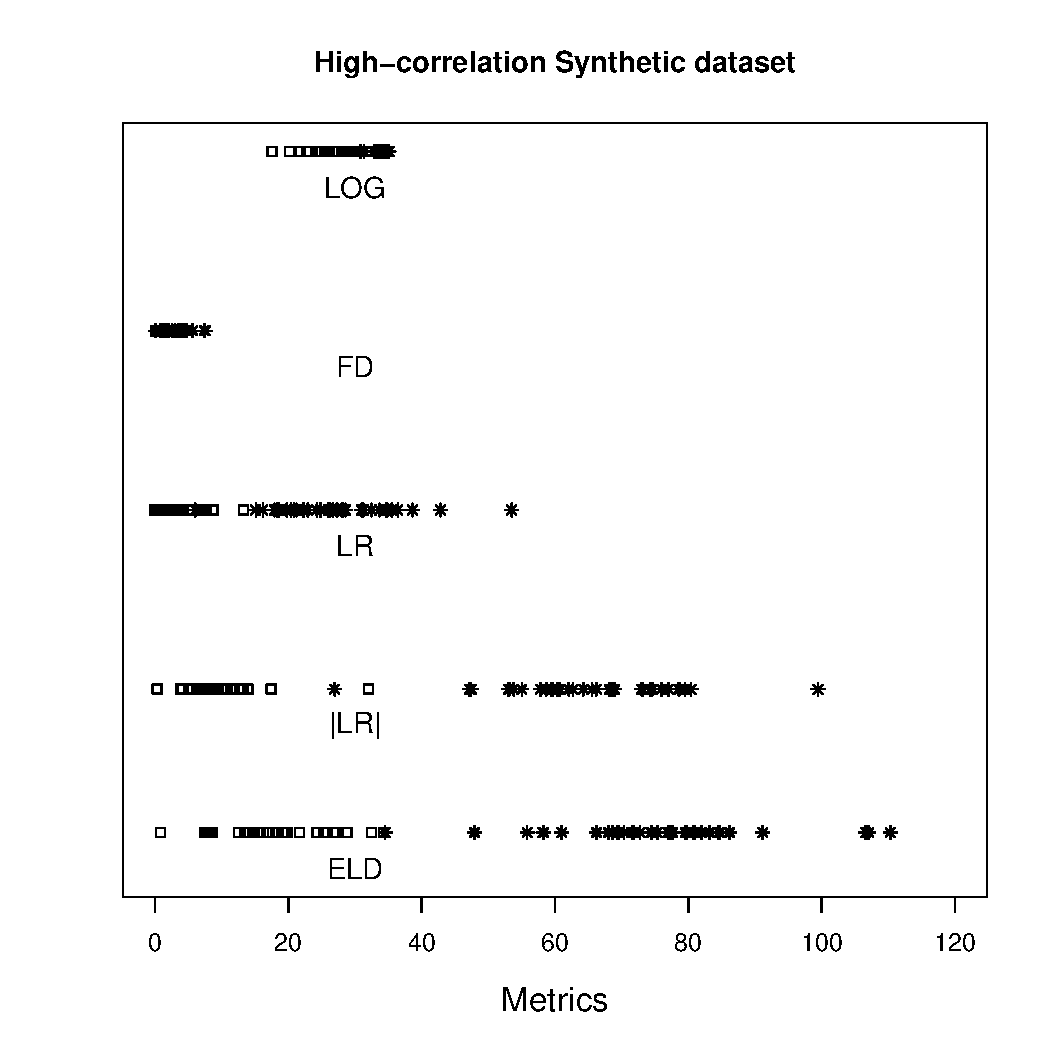
\includegraphics[width=2.5in]{DistributionPlots/sumSV-bk.pdf}
%										\caption{Distribution of different outlier scores in Synthetic Dataset- High correlation}
%										\label{fig:StrikerTime}
%									\end{minipage}
%								\end{figure}
%				
%				
%				
				
				

				
				
				%The advantages of succinctness and interpretability obtain also for computing scores. We write $B_{\object}$ for a BN that represents the object distribution, and $B_{\Class}$ for a BN that represents the class distribution. Then $\lr$ can be decomposed as $\lr = \sum_{i =1} ^{n} \lr_{i}$, where $$\lr_{i} = \sum_{j=1}^{\states_{i}} \sum_{\parents_{i}} \ln \frac{P_{B_{\object}}(\feature_{i} = \nodevalue_{ij}|\parents_{i})}{P_{B_{\Class}}(\feature_{i} = \nodevalue_{ij}|\parents_{i})}$$ where $\parents_{i}$ indexes all possible parent value combinations for node $\feature_{i}$, and the $P_{B}$ terms denote the conditional probability parameters of the applicable Bayesian network. In words, we sum over all possible child-parent states, and compute the log-probability ratio of the object and class conditional probabilities. The Bayesian network decompositions for the other scores are as follows. We compute feature score as before directly from the class and object distributions, rather than the Bayesian networks, since it concerns only marginal single-feature probabilities. 
				
				%\begin{eqnarray*} 
				%%\tag{$\lr(P_{\object}||P_{\Class})$} 
				%\eld_{i} & = & \sum_{j=1}^{\states_{i}} \sum_{\parents_{i}} |\ln \frac{P_{B_{\object}}(\feature_{i} = \nodevalue_{ij}|\parents_{i})}{P_{B_{\Class}}(\feature_{i} = \nodevalue_{ij}|\parents_{i})}|\\
				%\jid_{i} & = & \sum_{j=1}^{\states_{i}} \sum_{\parents_{i}} |\ln \frac{P_{B_{\object}}(\feature_{i} = \nodevalue_{ij}|\parents_{i})}{P_{\object}(\feature_{i})=\nodevalue_{ij}} - \ln \frac{P_{B_{\Class}}(\feature_{i} = \nodevalue_{ij}|\parents_{i})}{P_{\Class}(\feature_{i})=\nodevalue_{ij}}|\\
				%\mid_{i} & = &
				%\label{eq:eld}
				%\end{eqnarray*}
				
				
				
				
				
				%The learning algorithms were executed with 64-bit Centos with 4GB RAM and an Intel Core i5-480 M processor. 
				
				
				
				%\subsection{Outlier Metrics Compared}
				
				%\begin{description} 
				%We evaluate the outlier scores $\mid,\eld,\lr$ described in Section~\ref{sec:divergences}. 
				%
				%We use two existing baseline methods. 
				
				%\paragraph{Likelihood Method.} 
				%The metric $\lnlikelihood$ is defined by the equation:
				
				%\begin{equation*} \label{eq:ll}
				%\lnlikelihood_{i} = \sum_{j=1}^{\states_{i}} \sum_{\parents_{i}} P_{\object}(\feature_{i} = \nodevalue_{ij},%\parents_{i})\ln P_{\Class}(\feature_{i} = \nodevalue_{ij}|\parents_{i})
				%\end{equation*}
				
				%The intuition behind this metric is that the class distribution Bayesian network represents normal behavior\cite%{riahi2013}. An object is deemed an outlier if  the class BN assigns sufficiently low likelihood to generating %its features. Using low model likelihood to identify outliers is a common application of Bayesian networks \cite%{Cansado2008a}.  The equation above represents the standard BN log-likelihood function for the object data, %except that parent-child instantiation counts are standardized to be proportions. 
				%This avoids giving exponentially more influence to features with more groundings \cite{Schulte2011}. 
				
				
				%\item[\mid] The outlier metric is the Mutual Information Distance defined in Equation \eqref{eq:mid}. 
				%
				%\item[\eld] The outlier metric is the Mutual Information Distance defined in Equation \eqref{eq:eld}. 
				%
				%\item[\lr] The outlier metric is the KL divergence between the generic and the individual feature distribution. 
				%
				%\item[\lnlikelihood]  The outlier metric is the standardized log-likelihood $\lnlikelihood$ of the generic Bayesian network applied to the individual feature distribution. 
				%\marginpar{define, ranks everything the same on BN example (b).}
				%\item[\lr] The outlier metric is the likelihood ratio metric $\lr$. The Bayesian network learning method for the target individual's network uses the LAJ algorithm.
				
				%\item[
				
				%\paragraph{Local Outlier Factor.}
				
				%The local outlier factor is a popular density-based outlier metric that has been used as a baseline in previous %studies \cite{Breunig2000}. The metric requires specifying the number of nearest neighbors $k$. The authors of %the $\lof$ method recommend choosing a value between 10 and 20; we use 10 and 20.
				%\end{description}
				
				%$\lof$ requires as input a flat data matrix where each individual is represented by a single feature vector. To %aggregate features of individuals across complex objects such as matches or ratings, we use the total feature %count. This is the approach of the inventors of $\lof$ for sports data \cite{Breunig2000}. For example, they %counted the total number of goals scored by a player in a season as a feature for outlier analysis. We used the %implementation of $\lof$ in $\it{Data mining with R(DMwR)}$ package in R.
				
				%\subsection{Performance Metric} To score each outlier metric against ground truth instances, we follow the %%%approach of \cite{Gao2010,Cansado2008a}: Given the ground truth that $r\%$ of instances are outliers, we sort the outlier scores in descending order, and take the top $r\%$ as the outliers indicated by the method. We then report the true positive rate (recall), or \textbf{true outlier rate} (TOR), and the true negative rate, or \textbf{true normal rate} (TNR). The TNR is thus the percentage of normal individuals with rank below the top $r\%$. In anomaly detection the true outlier rate is the most important metric \cite{Gao2010,Cansado2008a}.
				

				\section{Experimental Evaluation and Comparison}~\label{sec:Experiments}
				%Details about our systems and algorithms that we use from previous work may be found in Section~\ref{sec:details}.  
				All the experiments were performed on a 64-bit Centos machine with 4GB RAM and an Intel Core i5-480 M processor. The likelihood-based outlier scores were computed with SQL queries using JDBC, JRE 1.7.0. and MySQL Server version 5.5.34.
				We utilized the synthetic datasets and real-world datasets from the soccer, hockey, movie and biology domains.
				
								
				%\begin{description}
				%\item[High Correlation]  See Figure~\ref{fig:synthetic-bns}(a).
				%\item[Low Correlation]  See Figure~\ref{fig:synthetic-bns}(b).
				%\item[Single attributes] See Figure~\ref{fig:synthetic-bns}(c).
				%\end{description}
				%
				
				

	\subsection{Synthetic Datasets}\label{sec:visual}
	We generated three synthetic datasets with normal and outlier players using the distributions represented in the three Bayesian networks of Figure~\ref{fig:synthetic-bns}. The main goal of designing synthetic experiments is to test the methods on  easy to detect outliers. 
	%We provide a 1D scatter plot for each outlier method to visualize the scores assigned to each player.
	 We used the $\it{mlbench}$ package in $\it{R}$ to generate synthetic features in matches, following these distributions for 240 normal players and 40 outliers. (There were 280 players in our Premier League dataset.) Each player participates in 38 matches, similar to the Premier League's real-world data. Each match assigns a value to each feature $F_1$ and $F_{2}$ for each player. This design yields the following three synthetic datasets. 
	\begin{description}
		\item\textbf{High Correlation}  Normal individuals exhibit a strong association between their features, outliers no association. Both normals and outliers have a close to uniform distribution over single features. See Figure~\ref{fig:synthetic-bns}(a).
		\item\textbf{Low Correlation}  Normal individuals exhibit no association between their features, outliers have a strong association. Both normals and outliers have a close to uniform distribution over single features. See Figure~\ref{fig:synthetic-bns}(b).
		\item\textbf{Single Features} Both normal and outlier individuals exhibit a strong association between their features. In normals, 90\% of the time, feature 1 has value 1. For outliers, feature 1 has value 1 only 10\% of the time. See Figure~\ref{fig:synthetic-bns}(c).
	\end{description}
	
%	Figure~\ref{fig:1DPlots} provides scatter plots for each synthetic dataset and each comparison outlier metric. The figure is best viewed on screen. As entailed by Proposition~\ref{prop:divergence}(Part \ref{clause:inequalities}), the $\mid$ metric maps players to the largest range of outlier scores. It also provides the best separation of normal from abnormal players: The normal players receive low anomaly scores and hence are clustered to the left of the $\mid$ scatter plot, whereas the abnormal players receive high scores and hence are clustered on the right. The $|\lr|$ metric  also shows a larger range of scores and a better discrimination compared to the $\lr$ metric. This illustrates the value of using distances rather than differences. In Section~\ref{sec:detection} we provide an aggregate detection accuracy score that quantifies this values.
	
	%	\textcolor{red}{maybe this example is too early}
		

\subsection{Real-world Datasets}\label{sec:real}  Our datasets and code are available on-line~\cite{url}. The following is the list of the real-world datasets we used in this work:
				\paragraph{Premier League Data} 
				The Opta data were released by Manchester City. 
				It lists box scores, that is, counts of all the ball actions within each game by each player, for the 2011-2012 season. 
				%The data consists of information about the actions of a single player in a given match 
				%from 2011 to 2012. 
				%Number of goals, passes, fouls, tackles, saves and blocks and also position 
				%assigned to a player in a match are examples of the information associated with each player. [list]
				%Information about the teams in a season, such as number of home wins, draws or away wins can be extracted by massaging the data. 
				%[The information can be visualized as a heterogeneous network that links players to teams, and teams to matches. ]
				For each player in a match, our data set contains eleven player features.
				% like $\it{TimePlayed}(\P,\M)$.
				For each team in a match, there are five features computed as player feature aggregates, as well as the team formation and the result (win, tie, loss). 
				There are two relationships, $\it{Appears\_Player}(\P,\M)$, $\it{Appears\_Team}(\T,\M)$. 
				%We store the data in a relational database, with a table for each base population and a table for each relationship.
				
Table~\ref{table:Features} lists the populations and features. Table~\ref{table:Stats} shows summary statistics for three of real-wolrd  datasets. 
\begin{table}
	\centering
	\resizebox{1\textwidth}{!}{
		\begin{tabular}{|l|l|l|l|l|l|} \hline
			\multicolumn{2}{|c|}{Premier League Statistics}& \multicolumn{2}{|c|}{IMDB Statistics}& \multicolumn{2}{|c|}{NHL Statistics}\\
			\hline
			Number of Teams&20&Number of Movies&3060&Number of Teams&30 \\ \hline
			Number of Players&484&Number of Directors&220&Number of Players& 921 \\ \hline
			Number of Matches&380&Number of Actors&98690&Number of Matches&720  \\ \hline
			avg player per match&26.01& avg actor per movie&36.42&avg player per match&29  \\ \hline
		\end{tabular} 
	}
	\caption{Summary Statistics for the IMDB and PL and NHL data sets}
	\label{table:Stats}
\end{table}


\begin{table}[htbp]
	\centering
	\resizebox{0.8\textwidth}{!}{
		\begin{tabular}{|c|p{5cm}|}
			\hline
			Individuals & Features\\ \hline
			\begin{tabular}{c}PL-Player\\per Match \end{tabular} & $\it{TimePlayed}$,$\it{Goals}$,$\it{SavesMade}$,
			$\it{ShotEff}$,$\it{PassEff}$,$\it{WinningGoal}$,
			$\it{FirstGoal}$,$\it{PositionID}$, $\it{TackleEff}$,$\it{DribbleEff}$,
			$\it{ShotsOnTarget}$ \\ \hline
			\begin{tabular}{c}PL-Team\\per Match \end{tabular} & $\it{Result}$,$\it{TeamFormation}$,
			$\sum\it{Goals}$,$\mu\it{ShotEff}$,$\mu\it{PassEff}$,
			$\mu\it{TackleEff}$,$\mu\it{DribbleEff}$. \\ \hline
			IMDB-Actor & $\it{Quality}$, $\it{Gender}$ \\ \hline
			IMDB-Director & $\it{Quality}$,$\it{avgRevenue}$\\ \hline
			IMDB-Movie&$\it{year}$,$\it{isEnglish}$,$\it{Genre}$,$\it{Country}$, $\it{RunningTime}$, $\it{Rating}$ by User\\ \hline
			IMDB-User& %$\it{Rating}$,
			$\it{Gender}$, $\it{Occupation}$.\\ \hline
				\begin{tabular}{c}NHL-Player\\per Match \end{tabular}&$\it{Goals}$,$\it{Assists}$,$\it{Points}$,$\it{PowerPlayTime}$,
				$\it{PlusMinus}$,$\it{Penalties}$,$\it{Shots}$,$\it{Hits}$,
				$\it{BlockedShots}$,$\it{Giveaways}$,
				$\it{ShotHandedTime}$,$\it{TimeOnIce}$\\ \hline
			\begin{tabular}{c}NHL-Team\\per Match \end{tabular} & $\it{Goals}$, $\it{GoalDifference}$\\\hline
		\end{tabular}}
		\caption{Attribute Features.% $\mu$ = average, $\\sum$ = sum. For relationships please see text.
			\label{table:Features}}
		
	\end{table}

				
				
				\paragraph{IMDb Data} 
				The Internet Movie Database (IMDb) is an on-line database of information related to films, television programs, and video games.
				The IMDb website offers a dataset containing information on cast, crew, titles, technical details and biographies into a set of compressed text files. 
				We preprocessed the data like \cite{Peralta2007} to obtain a database with seven tables: one for each population and one for the three relationships $\it{Rated}(\user,\movie)$, $\it{Directs}(\director,\movie)$, and $\it{ActsIn}(\actor,\movie)$.
				
				%				Table~\ref{table:Features} lists relationships and the number of features. 
				%				\begin{table}[htbp]
				%							\caption{Relationships and Example Features in Real-World Datasets.
				%								%For relationships please see text.
				%								\label{table:Features}}
				%					\centering
				%					\resizebox{0.3\textwidth}{!}{
				%						\begin{tabular}{|l|c|l|}
				%							\hline
				%							Path/Object Type & \#Attributes&Example\\ \hline
				%							\begin{tabular}{c}Player-Team-Match \end{tabular} & 11&ShotEff \\ \hline
				%							\begin{tabular}{c}Team-Match \end{tabular} & 7&TeamFormation \\ \hline\hline
				%							Actor & 2&Quality \\ \hline
				%							Director & 2&AvgRevenue\\ \hline
				%							Movie&5&Genre\\ \hline
				%							User& 2&Occupation\\ \hline
				%							User-Movie & 1&Rating \\\hline
				%							Actor-Movie & 1&Cast\_Position\\\hline
				%						\end{tabular}}
				%				
				%					\end{table}
				%\footnote{Commented table of relationships and features}
				%					\begin{LaTeXdescription}
				%						\item[Soccer Data]
				%						The Opta data were released by Manchester City. 
				%						It lists all the ball actions within each game by each player, for the 2011-2012 season.
				%						\item[IMDb Data]
				%						The Internet Movie Database (IMDb) is an online database of information related to films, television programs, and video games.
				%						The IMDb website offers a dataset containing information on cast, crew, titles, technical details and biographies in a set of compressed text files \cite{Peralta2007}.
				%					\end{LaTeXdescription}
				
				%\subsection{Outlier and Contrast Classes.}
				\paragraph{National Hockey League Data} 
				The NHL provides information about the sequences of play-by-play events. We used the data crawled by~\cite{schulte2014aggregating} that consists of the player game statistics for the seasons 2009-2013. The box scores summarize player statistics for each match, a total of 13 features. \\
				
				\paragraph{Mutagenesis Data}
				This dataset contains mutagenic activity of 188 compounds. 125 of these compounds have positive levels of log mutagenicity that are labelled ``active''.  The remaining compounds are labelled ``inactive'' and constitute the source of negative examples. In this dataset we considered examples of active compounds as the normal population and the inactive ones as the outlier. 
				
				\subsection{Evaluation Techniques for Outlier Detection}
				
				Measuring the effectiveness of outlier detection methods is not often an easy task. Most of the time ground truth information, that shows which data points are outliers, is unavailable. \\
				%In this section, we first discuss how outlier detection methods in the literature have tackled this problem, then we describe how we deal with it in our research.\\ 
				Several techniques have been employed in the literature to evaluate the performance of outlier detection methods:
				\begin{enumerate}
					\item Intuitive evaluation: case studies have been extensively used in the literature to evaluate outliers~\cite{aggarwal2013}. In Section~\ref{sec:CaseStudy} we use this method of evaluation for the top $n$ ranked detected outliers and we try to explain and make sense of the detected outliers. 	
					\item Synthetic data generation: another approach to evaluate anomaly detection methods is generating synthetic data and injecting synthetic outliers into the data~\cite{aggarwal2013}. We have designed and developed three synthetic datasets as discussed in section~\ref{sec:visual}.
					\item Anomaly injection: anomalies are injected into real-world datasets. Outlier detection methods are expected to detect the injected data points as outliers~\cite{Akoglu2015}. We employ this approach in our real-world datasets.
						In real-world data, there is no ground truth about which objects are outliers. To address this issue, we employ a one-class design: we learn a model for the class distribution, with data from that class only. 
						Then we rank all individuals from the normal class together with all objects from a contrast class treated as outliers, to test whether an outlier score recognizes objects from the contrast class as outliers.
						%		distinguishes objects from the normal class from objects in the contrast class. 
						Table~\ref{MetricComputation} shows the normal and contrast classes for three different datasets.  In-class outliers are possible, e.g. unusual strikers are still members of the striker class. Our case studies describe a few in-class outliers. In the soccer data, we considered only individuals who played more than 5 matches out of a maximum 38. For the three synthetic datasets, the scores are used to rank all 280 synthetic  players, 240 of which are normal and 40 are outliers.
					The disadvantage of this evaluation metric is that the real-world data may also contain anomalies, known as in-class outliers. However, this metric treats only the injected data points as true positives and will score anything other than those as false positives.
					%\item Internal Evaluation: in this type of evaluation outlier score has been used to quantify the extremity of data points~\cite{Pickands1975}.% We do not use this method of evaluation in our work.
				\end{enumerate}
			
	%			
				

				%The maximum number of matches played is 38.
				%
				%					In this design, we are only looking for the objects that are clearly deviating from the majority of the data. We are aware of the 
				
				%
				%\begin{description}
				%\item[Strikers vs. Goalies] The generic model is learned with match data from all 150 strikers. The outlier test cases are match data for all 22 goalies.
				%\item[Midfielder vs. Striker]  The generic model is learned with match data from all 172 midfielders. The outlier test cases are match data for 70 randomly selected strikers.
				%\item[Drama vs. Comedy] The generic model is learned with data for all 400 drama movies and 80 randomly selected comedy movies.
				%\end{description}
				%Figure~\ref{fig:synthetic} shows the true outlier rates for the different outlier metrics.  {\em On all datasets, the Mutual Information Score $\mid$ separates the normal class from the contrast class better than the other methods.} The same is true for the true negative rate; see supplementary file.
				%This rate reflects only the number of contrast objects that are ranked highly. Therefore we cannot expect a true outlier rate of 100\% because the normal class may also contain genuine outliers. If a metric correctly ranks these within-class outliers more highly than contrast class members, its TOR decreases. 
				% that are not in the contrast some strikers, may be genuine outliers within the striker class.
				
				\begin{table}
				
					\centering
					\resizebox{0.8\textwidth}{!}{
						\begin{tabular}{|l|c|l|c|}
							\hline
							Normal class&\#Normal&Outlier&\#Outlier class\\\hline
							Striker & 153 & Goalie&22\\ \hline
							Midfielder & 155 & Striker&74\\ \hline
							Drama & 197 & Comedy&47\\ \hline
							Defender & 186 & Forward&38\\ \hline
							Positive Compound&125&Negative Compound&63\\\hline
							%Synthetic&40&280\\ \hline
						\end{tabular}}	\caption{Outlier/normal Objects in Real-World Datasets. \label{MetricComputation}}
						
					\end{table}
					
					%						\subsection{Performance Score}
					%					 Our experiments provide empirical evidence that $\mid$ works better than other scores for object outlier detection.
					%						Our performance score for outlier rankings is the area under curve ($\auc$) of the well-established receiver operating characteristic $\roc$ curve.
					%						~\cite{Fawcett2006}. 
					%						This has been widely used to measure the performance of outlier ranking methods~\cite{Cansado2008, Muller2012}. The relationship between false positive rate (1- Specificity) and true positive rate (Sensitivity) is captured by the $\roc$ curve. Ideally, the best performance is achieved when we have the highest sensitivity and the highest specificity. 
					%					
					%						The maximum values for $\auc$ is 1.0 indicating a perfect ranking with 100\% sensitivity and 100\% specificity. In order to compute the $\auc$ value, we used the \textit{R} package \textit{ROCR}~\cite{RROCR2012}. Given a set of outlier scores, one for each object, this package returns an $\auc$ value. 
					%					
					
					\subsection{Methods Compared}
					\label{sec:methods}
					We compare three types of approaches, based on relational model likelihood, aggregation, and distance. 
					
\paragraph{Likelihood-based Outlier Scores.} The first approach evaluates the likelihood-based outlier scores described in Section~\ref{sec:metrics}. For relational Bayesian network structure learning we utilize the previous learn-and-join algorithm (LAJ), which is
					a state-of-the-art BN structure learning method for relational data \cite{Schulte2012}. The LAJ algorithm employs an iterative deepening strategy, which can be described as as search through a lattice of table joins. For each table join, different BNs are learned and the learned edges are propagated from smaller to larger table joins. 	For a full description, complexity analysis, and learning time measurements, please see \cite{Schulte2012}. 	We used the implementation of the LAJ algorithm due to its creators \cite{bib:jbnsite}. Of the likelihood-based scores, the likelihood ratio $\lr$ and our $\mid$ score fit in the EMM framework as they compare an object model with a population model. 
					
					%						probabilistic scores applied directly to the  data structured as an object tree. 
					\paragraph{Aggregation-based Methods.}
					The second approach first ``flattens" the structured data into a matrix of feature vectors, then applies standard matrix-based outlier detection methods. We refer to such methods as \textbf{aggregation-based}
					%Flattening the object data allows applying the rich set of matrix-based outlier detection methods ``as is" 
					(cf. Figures~\ref{fig:novelty}). For example, this was the approach taken by Breunig {\em et al.} for identifying anomalous players in sports data \cite{Breunig2000}. Following their paper, for each continuous feature in the object data, we use the average over its values, and for each discrete feature, we use the occurrence count of each feature value in the object data. Aggregation 
					tends to lose information about correlations.
					%\cite{DavidJensen2002}. 
					Our experiments address the empirical question of whether this loss of information affects outlier detection. 
					%The advantage to the aggregation approach is that after aggregating to preprocess the data, any matrix-based outlier detection method can be applied; see Figure~\ref{fig:flow}. 
					We evaluated three standard matrix-based outlier detection methods: Density-based $\lof$~\cite{Breunig2000}, distance-based $\knn$~\cite{Ramaswamy2000} and subspace analysis $\outrank$~\cite{Muller2012}.
					%\footnote{commented descriptions of these methods }. 
					These represent common, fundamental  approaches for vectorial data. 
					%	Subspace analysis is especially relevant to our study because 
					Like $\mid$, subspace analysis is sensitive to correlations among features. 
					% Our experiments applied $\outrank$ with two subspace clustering models, \textit{PRO-CLUS} \cite{Muller2012} and \textit{DISH} \cite{Kriegel2007}.  
					We used the available implementation of all three data matrix methods from the state of the art data mining software \textit{ELKI} \cite{Elke2013}. We used \textit{PRO-CLUS} as the clustering function for $\outrank$ as recommended by~\cite{Muller2012}.
					
						\paragraph{Relational Distance-based Method.}
						The third approach is based on a first-order distance measure that was developed and first used for the instance-based learning system RIBL2~\cite{Horvath2001}. This measure has proven  successful in several applications~\cite{Kirsten2001,Horvath1999}. We employ this metric and compute the distance between any two individuals in our population domain. Then, we rank the individuals based on their mean distance to the normal population.
					%	\subsubsection{Structured Data Methods}
					
					%						These include the $\mid$ and $\lr$ scores 
					%						that we introduced in Section~\ref{sec:metrics}. In addition, we apply the following two scores.
					%						
					%						
					%						
					%						 Including it as a baseline provides a lesion study for how important it is to consider the mutual information among attributes.
					%						Low model likelihood is a common score for using Bayesian networks to identify outliers \cite{Cansado2008}. The intuition behind the $\lnlikelihood$ score is that the class distribution Bayesian network represents normal behavior~\cite{riahi2013}. Low model likelihood therefore indicates anomalous objects. This is a common score for using Bayesian networks to identify outliers \cite{Cansado2008}.
					%An object is deemed an outlier if  the class BN assigns sufficiently low likelihood to generating its attributes.  
					%						The equation above represents the standard BN log-likelihood function for the object profile data, except that parent-child instantiation counts are standardized to be proportions \cite{Schulte2012}. 						
					%\subsubsection{Aggregation-based Matrix Methods}
					
					%%Standard outlier detection methods  require as input a flat data matrix where each individual is represented by a single attributes vector. To aggregate attributes of individuals across complex objects such as matches and ratings, we use the total attribute count. This is the approach that the inventors of $\lof$ \cite{Breunig2000} applied to sports data. For example they counted the total number of goals scored by a player in a season as a attribute for outlier analysis. 
					%						
					%For example, in the soccer dataset there is a correlation between ``shot efficiency" and ``dribble efficiency" of a striker and that correlation is a key feature to identify strikers from other class. However when we use the averages of these attributes,
					%%, by averaging over all the values of continuous attributes and counting the number of occurrences of different states of discrete attributes in all the player's matches, 
					%the correlation no longer exists. 
					% for comparison with $\mid$.
					%assume that the observations comprise independent data points that can be represented in a matrix. Since 
					%
					%Then, we study performance of \textit{MID} metric in comparison with:
					%\begin{description}
					%\item[$\lof$] is a density-based method originally presented in~\cite{Breunig2000} as a measure to quantify the outlier-ness of the data points relative to regions of different densities. Therefore, the score is defined based on local density instead of the nearest neighbor distance. In the simple words, $\lof$ compares the density of area around an object to the densities of the areas of the surrounding objects. However, $\lof$ defines density as the inverse of the average of the smoothed reachability distances in a neighborhood and this definition is not the precise definition of density in terms of number of data points within a specific region. $\lof$ is only sensitive to the density of the area and  ignore the orientation and the shape of the area.
					%\item[$\outrank$] is a subspace outlier ranking technique that employs the subspace analysis to identify the degree of outlierness. It compares clustered regions in different subspace and derive the outlierness score for each object. In this work we used $\outrank$ with two subspace clustering models \textit{PRO-CLUS} \cite{Muller2009} and \textit{DISH} \cite{Kriegel2007} (as suggested in~\cite{Muller2012} \textit{PRO-CLUS} is the best clustering function for their approach).
					%\item[$\knn$] is a well-known distanced-based outlier ranking method that is based on the distance of a point from its $k^{th}$ nearest neighbor and rank each object on the basis of its $k^{th}$ nearest neighbor. \cite{Ramaswamy2000}.
					%\end{description}
					
					%						\begin{LaTeXdescription}
					%							\item[$\lof$] is a standard density-based method~\cite{Breunig2000}.
					%							%It quantify the outlier-ness of the data points relative to regions of different densities. Therefore, the score is defined based on local density instead of the nearest neighbor distance. In the simple words, 
					%							$\lof$ compares the density of area around an object to the densities of the areas of the surrounding objects. 
					%							%However, $\lof$ defines density as the inverse of the average of the smoothed reachability distances in a neighborhood and this definition is not the precise definition of density in terms of number of data points within a specific region. $\lof$ is only sensitive to the density of the area and  ignore the orientation and the shape of the area.
					%							\item[$\knn$] is a well-known distanced-based outlier ranking method that assigns a score to each data point on the basis of distance of the point from its $k^{th}$ nearest neighbor ($D^k$) and  declare the top $n$ points as outliers~\cite{Ramaswamy2000}. 
					%							%They introduce a {\em partition-based} algorithm to set a upper bound and lower bound on $D^k$ to identify the partitions that cannot contain the top $n$ outliers and prune them in order to limit the search space. % \textbf{Sarah:more precise please}
					%							\item[$\outrank$] employs subspace analysis to measure the degree of outlierness. It compares clusters in different subspace to derive an outlier score for each object \cite{Muller2012}. \end{LaTeXdescription}
					
					%						Density and distance based methods are two fundamental approaches to outlier detection represented in our study by $\lof$ and $\knn$. Subspace analysis is a popular approach too, and relevant to our study because $\mid$ is sensitive to correlations among features as well. 
					
					
					\section{Empirical Results}
					
					We present results regarding computational feasibility, 
					%$\auc$ 
					predictive performance, and case studies.
					
					\subsection{Computational Cost of the $\mid$ Score.}
					%						
					%						Table~\ref{table:Number of Parameters} shows that the Bayesian network representation provides a highly compact summary of the target class distribution: the number of probabilities that need to be evaluated for computing the probabilistic scores decreases by a factor of 
					%						%\textbf{Sarah:fix dash}
					%						$10^{4}$\--$10^{5}$ depending on the dataset. 
					%						
					Table~\ref{table:LearningTime} shows that the computation of the $\mid$ value for a given target object is feasible. On average, it takes a quarter of a minute for each soccer player, and one minute for each movie. This includes the time for parameter learning from the object database.
					Learning the class model BN takes longer, but needs to be done only once for the entire object class. 
					{\em The BN model 
						%						is crucial for computational feasibility because it 
						provides a crucial %compact 
						low-dimensional representation of the 
						%joint 
						distribution information in the data.}
					% Table~\ref{table:Number of Parameters} compares the number of terms required to compute the $\mid$ score in the BN representation to the number of terms in an unfactored representation with one parameter for each joint probability $P(\Features = \set{\nodevalue})$ over all nodes.
					
					\begin{table}[htbp]
						\centering
						\begin{subtable}
							%\caption{Time for computing the $\mid$ metric. This includes the time for Bayes Net structure learning.\label{table:LearningTime}}
							\centering
			
							\resizebox{1\textwidth}{!}{
								\begin{tabular}{|l|l|l|} \hline
									Dataset& Class Model
									%    \begin{tabular}{c} Class \\Terms (min)\end{tabular}   & 
									%    \begin{tabular}{c} Object \\Terms (min)\end{tabular}   
									& Average per Object  \\ \hline
									PL: Strikers vs. Goalies&4.14&0.25\\ \hline
									PL: Midfielder vs. Goalies &4.02&0.25 \\ \hline
									IMDb: Drama vs. Comedy &8.30&1.00\\ \hline
									PL: Forward vs. Defender &5.30&0.35\\ \hline
									Mutagenesis: Positive Compound vs. Negative Compound &1.40&0.1\\ \hline
																		
								\end{tabular} 
							}
											\caption{Time (min) for computing the $\mid$ score. 
												%This includes the time for Bayes Net structure learning.
												\label{table:LearningTime}}
						\end{subtable}
						
%						\begin{subtable}
%							%\caption{The Bayesian network representation helps to decrease the number of terms that represent the class and object distributions. 
%							%For relationships please see text.
%							%\label{table:Number of Parameters}}
%							\centering
%							\caption{The Bayesian network representation decreases the number of terms required for computing the $\mid$ score.
%								%that represent the class and object distributions.
%								\label{table:Number of Parameters}}
%							\resizebox{0.8\textwidth}{!}{
%								\begin{tabular}{|l|l|l|}
%									\hline
%									Dataset & \begin{tabular}{c} \#Terms \\Using BN\end{tabular}  & \begin{tabular}{c} \#Terms \\ without Using BN
%									\end{tabular}\\ \hline
%									Strikers vs. Goalies & 1,430&114,633,792\\ \hline
%									Midfielders vs. Goalies & 1,376&43,670,016\\ \hline
%									Drama vs. Comedy & 50,802&215,040,000\\ \hline
%									Forward vs. Defender &1,756&180,657,332\\ \hline
%									Positive Compound vs. Negative Compound &NA&NA\\ \hline
%										
%								\end{tabular}
%							}
%							
%						\end{subtable}
						
					\end{table}


\subsection{Detection Accuracy} \label{sec:detection} Several accuracy scores have been developed to measure the performance of outlier ranking methods~\cite{aggarwal2013}. Arguably the most widely used score is the {\em area under curve} ($\auc$) of the receiver operating characteristic $\roc$ curve~\cite{Fawcett2006,Cansado2008,Muller2012}. 
%		This has been widely used to measure the performance of outlier ranking methods~\cite{Cansado2008,Muller2012}. 
		The relationship between false positive rate (1- Specificity) and true positive rate (Sensitivity) is captured by the $\roc$ curve. Ideally, the best performance is achieved when we have the highest sensitivity and the highest specificity. 
		%The area under the \textit{ROC} curve shows the overall performance and it is a measure to compare the curves numerically. 
		The maximum values for $\auc$ is, 1.0 indicating a perfect ranking with 100\% sensitivity and 100\% specificity. In order to compute the $\auc$ value, we used the \textit{R} package \textit{ROCR}~\cite{RROCR2012}. Given a set of outlier scores, one for each object, this package returns an $\auc$ value. 
%	Our experiments provide empirical evidence that in practice $\mid$ generally works better than other methods in all the Synthetic datasets and three out five real-world datasets.



	\paragraph{AUC Accuracy in Synthetic Datasets.}
	Table~\ref{table:Metric Comparison} shows the $\auc$ values for probabilistic methods and the outlier detection methods. On the synthetic data, it ought to be easy to distinguish the outliers and most methods detect most outliers well.  However, the EMM methods $\lr$ and $\mid$ are the only scores that achieves perfect or near perfect detection across all three synthetic datasets. $\it{RIBL}$ is the only method that fails in detecting outliers. $\it{RIBL}$ computes the distance between individuals by computing the distance of each instance of an individual to its nearest instance from other instances of the other individual. When comparing two individuals with only two binary features, $\it{RIBL}$ results in the same distance from the center of normal community for each individual.
	
	\paragraph{AUC Accuracy in Real-world Datasets.}
Table~\ref{table:proposMethod Comparison} shows the $\auc$ values
 %and table~\ref{table:Percision Comparison} shows precision 
 for aggregation-based methods compared to $\mid$ and $\it{RIBL}$ in the real-world datasets.  $\it{RIBL}$'s recursion depth bound is set to 2. The top performance of $\it{RIBL}$ and the model-based methods is substantially better than aggregation-based methods on all datasets,  confirming that it is important to develop outlier detection methods based on relational statistics for the relational data. The  EMM score $\mid$ works better than $\it{RIBL}$ or equally good in all the datasets except Midfielder vs. Strikers. In that dataset $\mid$ finds many in-class exceptional midfielders. However, $\it{RIBL}$ seems to perform better in distinguishing these two classes from each other. $\it{RIBL}$'s behavior in synthetic and real-world datasets suggests that when we have a small number of discrete features in our dataset, $\it{RIBL}$ may not be a good candidate to compute distance and hence outlier detection. But for numeric features it seems to be a good alternative.

Comparing the two EMM methods $\mid$ and $\lr$, using distance rather than expectation allows $\mid$ to achieve a substantially higher AUC than $\lr$ on all datasets except for the NHL. On the NHL dataset, the $\lr$ metric outperforms both $\it{RIBL}$ and $\mid$, which is an example of how taking absolute values does not alway result in better detection performance.   

On the synthetic data, we compare the two EMM methods further  with precision@r\% another metric used in a previous study on relational outlier detection~\cite{Gao2010}, which is computed as follows: 1) Sort the outlier scores obtained by an outlier ranking method in descending order. 2) Return the fraction of the top $r$ percent that are in fact outliers. Precision@r\% focuses on the ability to detect clear outliers. As Table~\ref{table:Percision Comparison} shows, the $\mid$ score is the best for this metric.
	%We evaluate the performance of $\mid$ compared to other outlier different metrics.

	\begin{table}
		\begin{subtable}
			
			\centering
			\resizebox{1\textwidth}{!}{
			%	\begin{tabular}{|l|l|l|l|l|l|l|l|l|l|}
			\begin{tabular}{|l|l|l|l|l|l|l|l|l|}
					\hline
					Dataset & \underline{\mid}&\loglikelihood&\underline{\lr}&$FD$&\it{RIBL}&$\lof$&\it{OutRank}&\begin{tabular}{c}\it{KNN}\\\it{Outlier}\end{tabular}\\ \hline
					
					High Correlation & \textbf{1.00}&0.99&0.97&0.89&0.50&0.68&0.99&0.97 \\ \hline
					Low Correlation & \textbf{1.00}&0.97&0.99&0.42&0.50&0.58&0.83&0.97 \\ \hline
					Single Feature & \textbf{1.00}&0.79&\textbf{1.00}&\textbf{1.00}&0.50&0.63&0.88&0.86 \\ \hline
					%Strikers vs. Goalies & \textbf{0.89} &0.77&0.65&0.71& 0.61\\ \hline
					%Midfielders vs. Strikers &\textbf{0.66}&{0.62} &0.55 &0.59&0.45 \\ \hline
					%Drama vs. Comedy & \textbf{0.70} &0.68&0.66&0.64&0.66 \\ \hline
				\end{tabular}}
				\caption{AUC of the $\mid$ Outlier detection methods in Synthetic datasets. The EMM methods are underlined. %ND stands for ``no detection''.
					%For relationships please see text.
					\label{table:Metric Comparison}}
			\end{subtable}
			
			
			
			\begin{subtable}
				
				\centering
				\resizebox{1\textwidth}{!}{								 							 			\begin{tabular}{|l|c|c|c|c|c|c|c|c|}
						\hline
    						Dataset & \underline{\mid}&\loglikelihood&\underline{\lr}&$FD$&\it{RIBL}&$\lof$&\it{OutRank}&\begin{tabular}{c}\it{KNN}\\\it{Outlier}\end{tabular}\\ \hline
PL: Strikers vs. Goalies & \textbf{0.89} &0.61&0.65&0.61&0.71&0.61&0.60&0.61 \\ \hline 
PL: Midfielders vs. Strikers  &0.66 &0.45&0.55&0.59&\textbf{0.78}&0.76 &0.71&0.58 \\ \hline
IMDb: Drama vs. Comedy & 	\textbf{0.70} &0.66&0.66&0.64&\textbf{0.70}&0.51&0.68&0.68 \\\hline
  NHL: Defender vs. Forward & 0.78&0.58& \textbf{0.87}&0.79&0.71&0.73&0.73&0.66 \\ \hline
   Mutagenesis: Positive vs Negative & \textbf{0.86} &0.64&0.81&0.70&0.70&0.51&0.57&0.53 \\\hline
					\end{tabular}}
					\caption[AUC of the $\mid$ vs. other outlier detection methods.]{AUC  outlier detection methods in real-world datasets.						%For relationships please see text.
						\label{table:proposMethod Comparison}}
				\end{subtable}
			\end{table}
			
%OS switched RIBL and Log column to be consistent with table 10 for synthetic data
															
		\begin{table}
		\caption{Precision@r\% of Outlier detection methods in Synthetic datasets.
			\label{table:Percision Comparison}}
		    \resizebox{1\textwidth}{!}{	
				\begin{tabular}{|l|c|c|c|c|c|c|c|c|c|}\hline
					Dataset & Percentage & \underline{\mid}&\loglikelihood&\underline{\lr}&$FD$&$\lof$&\it{OutRank}&\begin{tabular}{c}\it{KNN}\\\it{Outlier}\end{tabular}\\ \hline																																				\multirow{2}{*}{High-Correlation}& 1\%& \textbf{1.00}& 0.91& 0.73& 0.47& 0.11& 0.53& 0.48\\
					&5\%&\textbf{1.00}&0.95&0.85&0.65&0.22&0.50&0.65\\	\hline																				    	 \multirow{2}{*}{Low-Correlation}& 1\%& \textbf{1.00}& 0.93& 0.87& 0.14& 0.10& 0.00& 0.06\\
					&5\%&\textbf{1.00}&0.95&0.90&0.25&0.25&0.10&0.57\\\hline
			   	\multirow{2}{*}{Single-Feature}& 1\%& \textbf{1.00}& 0.81& \textbf{1.00}& \textbf{1.00}& 0.46& \textbf{1.00}& 0.51\\
				&5\%&\textbf{1.00}&0.89&\textbf{1.00}&\textbf{1.00}&0.55&\textbf{1.00}&0.54\\	\hline    
%																		\multirow{2}{*}{Striker-Goalie}& 5\%& \textbf{0.57}& 0.27& 0.22& 0.51& 0.36& 0.19& 0.47& 0.42\\
%																		&15\%&\textbf{0.63}&0.36&0.31&0.58&0.40&0.32&0.50&0.52\\
%																		\hline    
%																		\multirow{2}{*}{Midfielder-Striker}& 1\%&\textbf{ 0.49}& 0.42& 0.25& 0.41& 0.46& 0.29& 0.44& 0.16\\
%																		&5\%&\textbf{0.52}&0.48&0.39&0.44&0.50&0.38&0.48&0.35\\
%																		\hline  																				\multirow{2}{*}{Drama-Comedy}&1\%& \textbf{0.44}& 0.38& 0.39& 0.15& 0.22& 0.29& 0.07& 0.014\\
%																		&5\%&\textbf{0.47}&0.45&0.44&0.40&0.28&0.36&0.17&0.20\\
%																		\hline     
																			\end{tabular}	}		
																	
																\end{table}
																
																{\em Conclusion.} The outlier detection methods with the best over all performance are the two based on the Exceptional Model Mining Framework, using the traditional log-likelihood ratio (or Kulback-Leibler divergence), and our novel expected log-distance metric $\mid$. While the $\mid$ score does not uniformly outperform $\lr$, the improvement is frequent and substantial enough to recommend it as an alternative for practical applications. 
%\paragraph{Probabilistic Structured methods:}

%\paragraph{Propositionalization-Based Methods vs. \mid} 
%Table~\ref{table:proposMethod Comparison} shows the precision values for propositional-based methods compared to $\mid$. {\em Our $\mid$ score outperforms all Propositional-based methods on all datasets}, except for one real-world dataset that $\lof$ outperform $\mid$ and that is with the help of conjunctive features generated by the  propositionalization method introduced in chapter~\ref{chap:four}. If we use aggregated features the performance of $\lof$ drops to 0.53. In general, if we use aggregated features, as used in the literature to generate features for the baseline methods,
%%								Comparing tables~\ref{table:Metric Comparison} and~\ref{table:Method Comparison} shows that t
%the performance of propositional-based methods are most like that of the probabilistic score $\fd$, which does not consider the
%correlation among the features.
%					


%					\subsection{Detection Accuracy} \label{sec:detection} We follow the evaluation design of~\cite{Gao2010} and 
%					make each baseline methods detect the same percentage of  objects as outliers:
%					% as that of the ground-truths. To achieve this, we 
%					Sort the outlier scores obtained by the three baseline methods in descending order, and take the top $r$ percent as outliers. Then we use \textbf{precision}, a.k.a. \textbf{true positive rate} as the evaluation metric which is the percentage of correct ones in the set of outliers identified by the algorithm. As in~\cite{Gao2010}, we set the percentages of outlier to be 1\% and 5\%. In the one-class design, precision measures how many members of the outlier class were correctly recognized. We also report some AUC measurements \cite{aggarwal2013}, which aggregate precision values at different percentage cutoffs.\footnote{Our $\mid$ score performs the best also with other metrics such as recall, to a similar degree.} %\textbf{Sarah: I'd love to have the plots of all points here.}
%					
%					
%					\paragraph{Likelihood-Based Methods} 
%					
%					
%					Table~\ref{table:Method Comparison} shows the $\auc$ values for each probabilistic ranking. {\em Our $\mid$ score achieves the top score on each dataset.} On the synthetic data, $\mid$ and $|\lr|$ are the only scores with 100\% precision at 1\% and 5\%. This confirms the value of using distances rather than differences. 
%					%						However, the AUC score shows that $\mid$ retains perfect detection with different percentage cutoffs, but $|\lr|$ ranks some normal objects higher than actual outliers. 
%					While it ought to be easy to distinguish the outliers, Table~\ref{table:Metric Comparison} shows that {\em $\mid$  is the only score that achieves perfect detection}, that is AUC = 1.0.
%					
%					%\footnote{\textbf{Sarah}: in the table LR is perfect as well. That's because we only look at precision, right?} 
%					%For this reason, in Table~\ref{table:Method Comparison} we compare only the performance of $\mid$ to the previous data matrix methods.
%					%						\begin{table}
%					%							\begin{subtable}
%					%								
%					%								\centering
%					%									\caption{$\auc$ of $\mid$ vs. other probabilistic scores. 
%					%										%For relationships please see text.
%					%										\label{table:Metric Comparison}}
%					%								\resizebox{1\textwidth}{!}{
%					%									
%					%									\begin{tabular}{|l|l|l|l|l|}
%					%										\hline
%					%										Dataset & \mid &\lr &\fd&\lnlikelihood\\ \hline
%					%										
%					%										Synthetic Data-High Correlation & \textbf{1.00}&0.95&0.88&0.98 \\ \hline
%					%										Synthetic Data-Low Correlation & \textbf{1.00}&0.95&0.35&0.95 \\ \hline
%					%										Synthetic Data-Single Feature & \textbf{1.00}&0.89&0.79&0.98 \\ \hline
%					%										Real Data-Strikers vs. Goalies & \textbf{0.89} &0.61&0.83& 0.65\\ \hline
%					%										Real Data-Midfielders vs. Strikers &\textbf{0.66} &0.64 &0.52&0.64 \\ \hline
%					%										Real Data-Drama vs. Comedy & \textbf{0.70} &0.65&0.61&0.63 \\ \hline
%					%									\end{tabular}}
%					%								
%					%								\end{subtable}
%					%								
%					%								\begin{subtable}
%					%									
%					%									\centering
%					%										\caption{$\auc$ of $\mid$ vs. aggregation-based Outlier Ranking Methods. 
%					%											%For relationships please see text.
%					%											\label{table:Method Comparison} 
%					%										}
%					%									\resizebox{1\textwidth}{!}{
%					%										\begin{tabular}{|l|c|c|c|c|c|}
%					%											\hline
%					%											Dataset & $\mid$ &$\lof$&\begin{tabular}{c}$\outrank$\\(ProClus)\end{tabular}&\begin{tabular}{c}$\outrank$\\(DISH)\end{tabular}&\begin{tabular}{c}\it{KNN}\\\it{Outlier}\end{tabular}\\ \hline
%					%											
%					%											High Correlation & \textbf{1.00}&0.87&0.73&0.95&0.92 \\ \hline
%					%											Low  Correlation & \textbf{1.00}&0.53&0.33&0.32&0.45 \\ \hline
%					%											Single Feature & \textbf{1.00}&0.58&1.00&0.96&0.95\\ \hline
%					%											Strikers vs. Goalies & \textbf{0.89} &0.68&0.89&0.53&0.75 \\ \hline
%					%											Midfielders vs. Strikers &\textbf{0.66} &0.53 &0.54&0.49&0.55 \\ \hline
%					%											Drama vs. Comedy & \textbf{0.70} &0.53&0.56&0.42&0.61 \\ \hline
%					%										\end{tabular}}
%					%									
%					%									\end{subtable}
%					%								\end{table}
%					%											\begin{table}
%					%									
%					%															\caption{Precision of $\mid$ compare to other baseline scores in different datasets
%					%																\label{table:CaseStudy}}
%					%															\resizebox{1\textwidth}{!}{	
%					%															\begin{tabular}{|l|c|c|c|c|c|c|c|c|}\hline
%					%																	Dataset&\multicolumn{5}{|c|}{Structured-based models }&\multicolumn{3}{|c|}{Aggregation-based models}\\
%					%																	\hline
%					%																 &\mid&$|KLD|$&\lr&\fd&\lnlikelihood&\lof&$\outrank$	&\knn\\
%					%																	\hline
%					%																	High-Correlation &\textbf{1.00}&\textbf{1.00}&0.85&0.65&0.95&0.22&0.50&0.65\\
%					%																	\hline	
%					%																	Low-Correlation&\textbf{1.00}&\textbf{1.00}&0.90&0.25&0.95&0.25&0.10&0.10\\
%					%																	\hline
%					%																	Single-Feature&\textbf{1.00}&\textbf{1.00}&0.55&0.62&0.92&0.55&1.00&0.67\\\hline
%					%																	Striker-Goali&\textbf{0.63}&0.36&0.31&0.58&0.40&0.32&0.50&0.52\\\hline
%					%																	Midfielder-Striker&\textbf{0.52}&0.50&0.39&0.44&0.50&0.38&0.48&0.35\\\hline
%					%																	Drama-Comedy&\textbf{0.47}&0.45&0.44&0.40&0.28&0.36&0.17&0.20\\\hline
%					%																\end{tabular}	}		
%					%																	
%					%												\end{table}
%					
%					\begin{table}
%						\caption{Precision of outlier scores in different datasets.
%							\label{table:Method Comparison}}
%						\resizebox{1\textwidth}{!}{	
%							\begin{tabular}{|l|c|c|c|c|c|c|c|c|c|}\hline
%								Dataset& percentage&\multicolumn{5}{|c|}{Model-based models }&\multicolumn{3}{|c|}{Aggregation-based models}\\
%								\hline
%								& &\mid&$|\lr|$&\lr&\fd&\loglikelihood&\lof&$\outrank$	&\knn\\
%								\hline
%								\multirow{2}{*}{High-Correlation}& 1\%& \textbf{1.00}& \textbf{1.00}& 0.73& 0.47& 0.91& 0.11& 0.53& 0.48\\
%								&5\%&\textbf{1.00}&\textbf{1.00}&0.85&0.65&0.95&0.22&0.50&0.65\\\hline			
%																										    	 \multirow{2}{*}{Low-Correlation}& 1\%& \textbf{1.00}& \textbf{1.00}& 0.87& 0.14& 0.93& 0.10& 0.00& 0.06\\
%								&5\%&\textbf{1.00}&\textbf{1.00}&0.90&0.25&0.95&0.25&0.10&0.14\\
%								\hline
%								\multirow{2}{*}{Single-Feature}& 1\%& \textbf{1.00}& \textbf{1.00}& 0.39& 0.53& 0.81& 0.46& \textbf{1.00}& 0.51\\
%								&5\%&\textbf{1.00}&\textbf{1.00}&0.55&0.62&0.92&0.55&\textbf{1.00}&0.54\\
%								\hline    
%								\multirow{2}{*}{Striker-Goalie}& 5\%& \textbf{0.57}& 0.27& 0.22& 0.51& 0.36& 0.19& 0.47& 0.42\\
%								&15\%&\textbf{0.63}&0.36&0.31&0.58&0.40&0.32&0.50&0.52\\
%								\hline    
%								\multirow{2}{*}{Midfielder-Striker}& 1\%&\textbf{ 0.49}& 0.42& 0.25& 0.41& 0.46& 0.29& 0.44& 0.16\\
%								&5\%&\textbf{0.52}&0.48&0.39&0.44&0.50&0.38&0.48&0.35\\
%								\hline  													\multirow{2}{*}{Drama-Comedy}&1\%& \textbf{0.44}& 0.38& 0.39& 0.15& 0.22& 0.29& 0.07& 0.014\\
%								&5\%&\textbf{0.47}&0.45&0.44&0.40&0.28&0.36&0.17&0.20\\
%								\hline     
%							\end{tabular}}		
%							
%						\end{table}
						
						%						\begin{table}
						%							\centering
						%								\caption{\textit{AUC} of $\mid$ vs. $|LR|$. 
						%									%For relationships please see text.
						%									\label{table:Metric Comparison}}
						%							\resizebox{0.3\textwidth}{!}{
						%								\begin{tabular}{|l|l|l|}\hline
						%									Dataset & \mid &$|\lr|$\\ \hline
						%									Synthetic Data-High Correlation & \textbf{1.00}&0.95 \\ \hline
						%									Synthetic Data-Low Correlation & \textbf{1.00}&0.95 \\ \hline
						%									Synthetic Data-Single Feature & \textbf{1.00}&0.89 \\ \hline
						%%									Real Data-Strikers vs. Goalies & \textbf{0.89} &0.61\\ \hline
						%%									Real Data-Midfielders vs. Strikers &\textbf{0.66} &0.64 \\ \hline
						%%									Real Data-Drama vs. Comedy & \textbf{0.70} &0.65 \\ \hline
						%								\end{tabular}}
						%							
						%							\end{table}
						%					\begin{table}
						%						\centering
						%						\caption{\textit{AUC} of $\mid$ vs. $|LR|$. 
						%							%For relationships please see text.
						%							\label{table:Metric Comparison}}
						%						\resizebox{1\textwidth}{!}{
						%							\begin{tabular}{|l|l|l|l|l|l|l|}\hline
						%								Score & high-Cor. &Low-Cor.&Single-Fe.&Striker&Midfielder&Drama\\ \hline
						%								 \mid&1.00&1.00&1.00&0.89&0.66&0.70\\\hline
						%								$|\lr|$&0.95&0.95&0.89&0.61&0.64&0.65\\\hline
						%							%	Synthetic Data-High Correlation & \textbf{1.00}&0.95 \\ \hline
						%							%	Synthetic Data-Low Correlation & \textbf{1.00}&0.95 \\ \hline
						%							%	Synthetic Data-Single Feature & \textbf{1.00}&0.89 \\ \hline
						%								%									Real Data-Strikers vs. Goalies & \textbf{0.89} &0.61\\ \hline
						%								%									Real Data-Midfielders vs. Strikers &\textbf{0.66} &0.64 \\ \hline
						%								%									Real Data-Drama vs. Comedy & \textbf{0.70} &0.65 \\ \hline
						%							\end{tabular}}
						%							
						%						\end{table}
						
						

							
%								
%							\paragraph{Aggregation-Based Methods vs. \mid} 
%							Table~\ref{table:Method Comparison} shows the precision values for aggregation-based methods compared to $\mid$. {\em Our $\mid$ score outperforms all aggregation-based methods on all datasets}, except for a tie with $\outrank$(ProClus) on the relatively easy problem of distinguishing strikers from goalies.
%							%								Comparing tables~\ref{table:Metric Comparison} and~\ref{table:Method Comparison} shows that t
%							The performances of aggregation-based methods are most like that of the probabilistic score $\fd$, which does not consider the
%							correlation among the features. This finding reflects the fact that aggregation tends to lose information about correlations.
%							% \cite{DavidJensen2002}. 
%							The aggregation-based methods achieve their highest performance on the Strikers vs. Goalies dataset. In this dataset action count features such as ShotsOnTarget, ShotEfficiency point to strikers and the feature SavesMade points to goalies. Therefore, outliers in this dataset are easy to find by considering features in isolation.
							%\\
							%\\
							%Based on the results shown in table ~\ref{table:Method Comparison}, the easiest dataset is Single Features, as most of the methods are successful in detecting outliers in that dataset. The low correlation dataset seems to be the most challenging one. 
							%The results of $\knn$ seem to be closest to $\mid$ in most datasets. 
							
							%The $\roc$ curve in Figure~\ref{fig:ROC} shows the performance of $\mid$ and $\knn$ which indicates that $\mid$ always reaches a higher true positive rate earlier that $\knn$.
							%\textbf{Sarah: both graph and table?}
							%Show the running time in a table. Explain that thats one of the weakness of $\mid$ compare to the others. But since the its performance is much higher than the compatitors it is worth the waiting!
							
							%
							%
							%
							%Strikers vs. goalies dataset is very similar to synthetic dataset, single feature in a sense that outlier and normal classes in both datasets contain single features that have distinct and very different distributions independent of the other attributes. In Strikers vs. Goalies attributes such as ShotsOnTarget or ShotEfficiency are valid only if the object is a member of Striker class and SavesMade only belongs to Goalie Class. Therefore, outliers in this dataset are also very easy to find even by applying the aggregation-based methods.  
							
							
							
							%\begin{figure*}
							%\centering
							%\resizebox{0.9\textwidth}{!}{
							
							%\subfigure{
							%  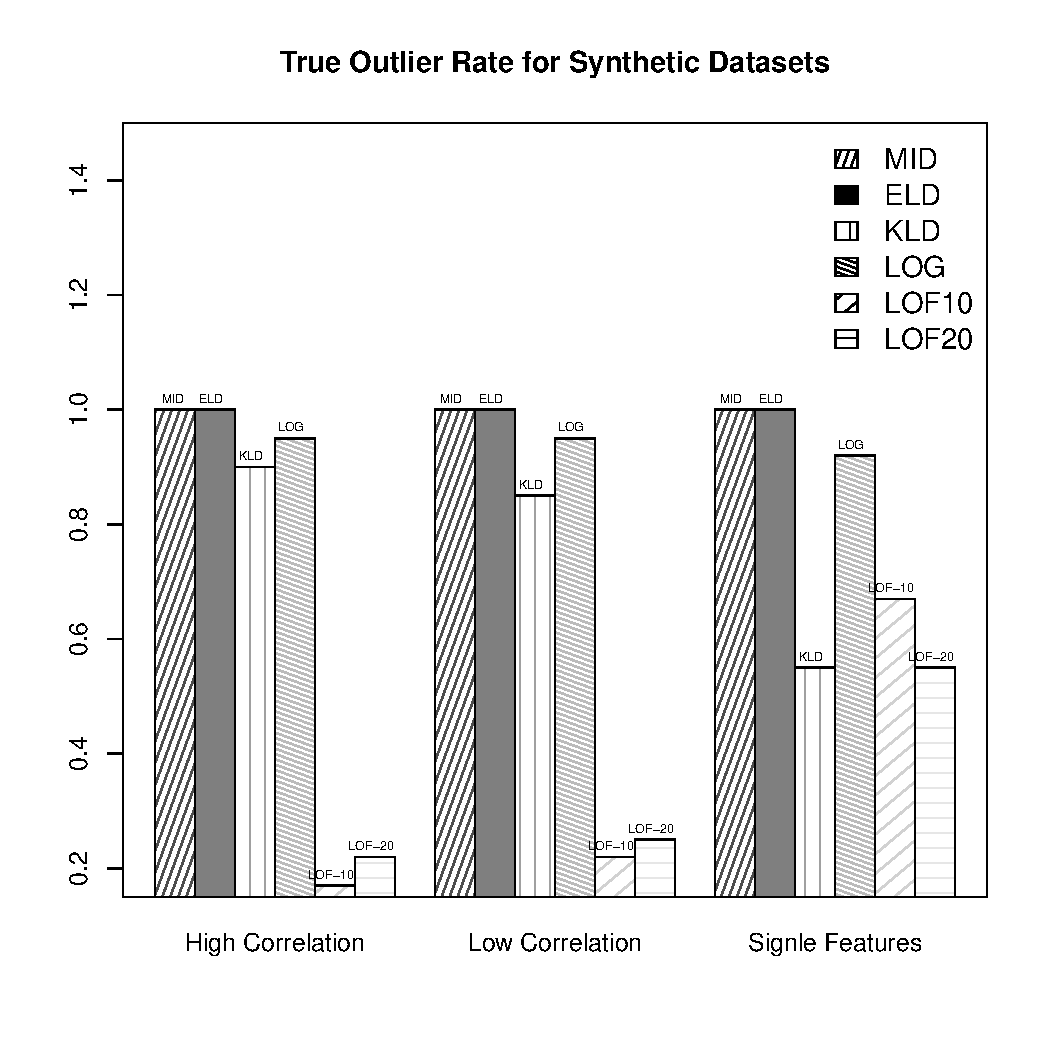
\includegraphics[height=70mm, width=70mm] {figures/TPR-Synthetic.pdf}
							%}
							%\subfigure{
							%  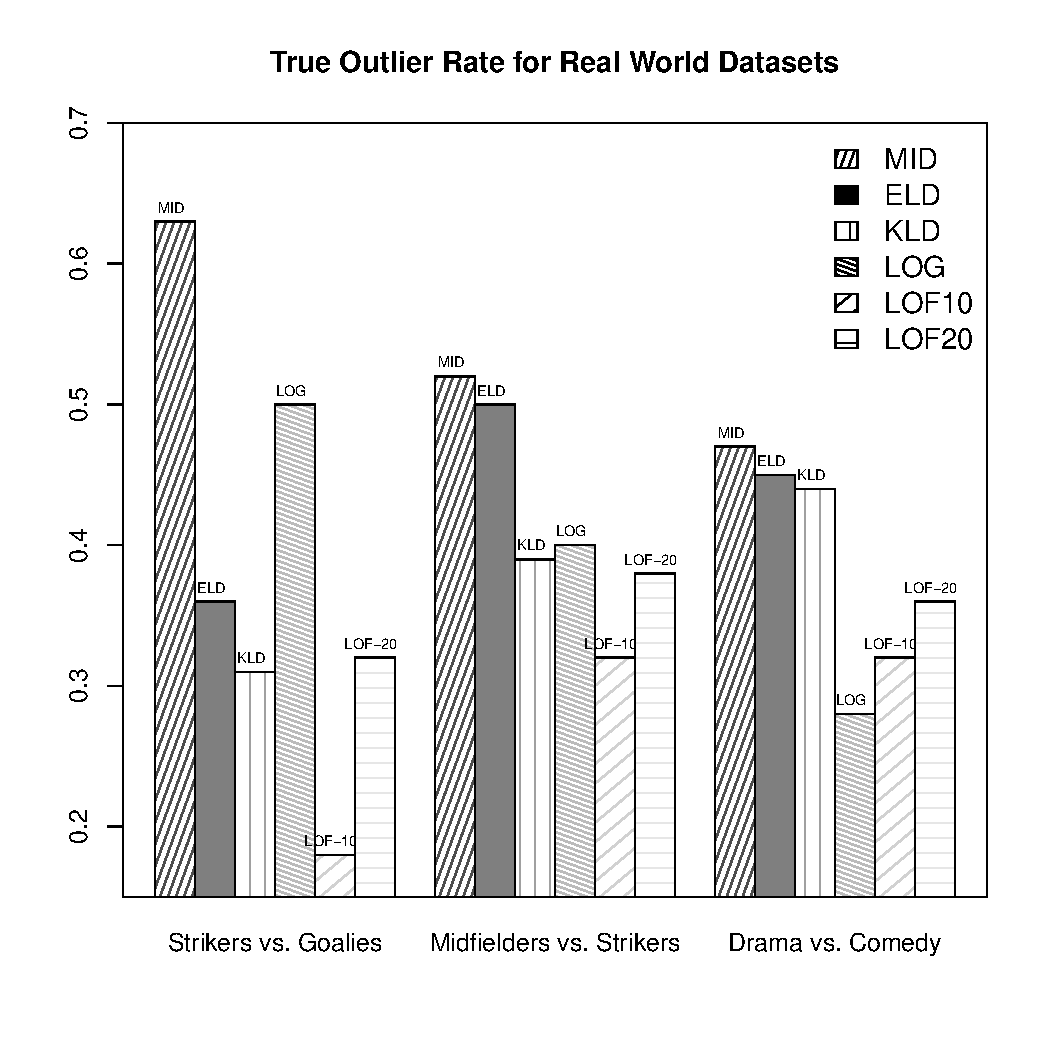
\includegraphics[height=70mm, width=70mm] {figures/TPR-All.pdf}
							
							% }
							% }
							
							%\caption{Comparison of Object Outlier Metrics}
							%\label{fig:synthetic}
							%\end{figure*}
							
							\subsection{Case Studies} \label{sec:CaseStudy} For a case study, we examine the three top outliers as ranked by $\mid$, shown in Table~\ref{table:CaseStudy}. 
							The aim of the case study is to provide a qualitative sense of the outliers indicated by the scores. Also, we illustrate how the BN representation leads to an interpretable ranking. 
							Specifically, we employ a {\em feature-wise decomposition} of the score combined with a {\em drill down} analysis: 
							
							\begin{enumerate}
								\item Find the node $\feature_{i}$ that has the highest $\mid_{i}$ divergence score for the outlier object. 
								\item Find the parent-child combination that contributes the most to the $\mid_{i}$ score for that node.
								\item Decompose the $\mid$ score for the parent-child combination into feature and mutual information component. 
							\end{enumerate}
							
							We present strong associations---indicated by the $\mid$'s mutual information component---in the intuitive format of association rules. This analysis can also be applied to $\lr$ using the form~\eqref{eq:decompose}; we focus on $\mid$ for compactness.
							
							%\begin{figure}
							%\centering
							%   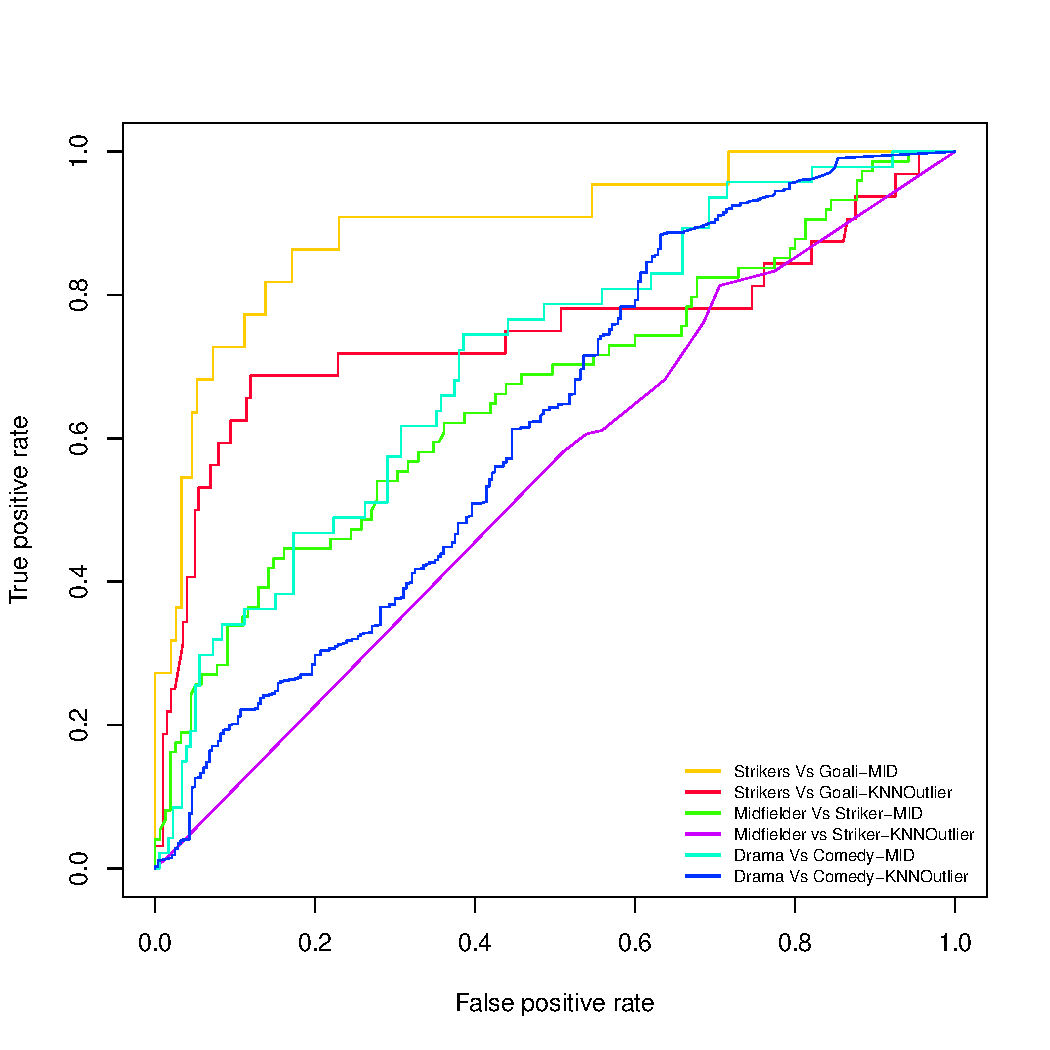
\includegraphics[width=1\textwidth] {figures/ROCKNN.pdf}
							% \caption{Detection Accuracy of $\mid$ vs. $\knn$
							% \label{fig:ROC}}
							%\end{figure}
							%\vspace{-5mm}
							\paragraph{Strikers vs. Goalies} 
							%The Mutual Information Score $\mid$ separates goalies from Strikers better compared to the other methods.  
							%
							In real-world data, a rare object may be a {\em within-class outlier}, i.e., highly anomalous even within its class. In an unsupervised setting without class labels, we do not expect an outlier score to distinguish such an in-class outlier from outliers outside the class. 
							%								This is the reason why in real-world data, we do not expect an outlier detection score to distinguish the normal class objects perfectly from objects outside the class. 
							An example is the striker Edin Dzeko. He is a highly anomalous striker who obtains 
							the top $\mid$ divergence score among both strikers and goalies. His $\mid$ score is highest for the Dribble Efficiency feature. The highest $\mid$ score for that feature occurs when Dribble Efficiency is low, and its parents have the following values: Shot Efficiency high, Tackle Efficiency medium. Looking at the single feature divergence, 
							%Decomposing this $\mid$ score into feature divergence and joint information divergence, 
							we see that Edin Dzeko is indeed an outlier in the Dribble Efficiency subspace: His dribble efficiency is low in 16\% of his matches, whereas a randomly selected striker has low dribble efficiency in 50\% of their matches. Thus, Edin Dzeko is an unusually good dribbler. Looking at the mutual information component of $\mid$, i.e., the parent-child correlations, for Edin Dzeko the confidence of the rule 
							$$\it{ShotEff} = \it{high}, \it{TackleEff} = \it{medium}\rightarrow \it{DribbleEff} = \it{low}$$ is 50\%, whereas in the general striker class it is $38\%$.
							%The $\eld$ divergence also ranks Edin Dzeko as unusual. But because it allows feature and joint information divergence to cancel, his rank is somewhat lower. The likelihood metric does not recognize him as unusual at all. 
							
							%								The next two outliers according to $\mid$ are goalies Paul Robinson and Michel Vorm. Their rank is based only on feature divergence, with zero mutual information distinction. The maximum feature divergence is obtained by the $\it{SavesMade}$ feature. This makes intuitive sense since strikers basically never make saves. 
							%In other words, feature divergence with respect to $\it{SavesMade}$ is a good way to distinguish goalies from strikers. 
							%
							%The $\eld$ divergence also ranks Paul Robinson and Michel Vorm as clear goalies.  The likelihood metric does not recognize Paul Robinson as unusual at all. 
							%\vspace{-5mm}
							\paragraph{Midfielders vs. Strikers} 
							%The  $\mid$ metric separates midfielders from strikers better compared than the other methods.  
							%The single feature divergence does not discriminate these two classes of objects. Intuitively, this is because strikers and midfielders are generally similar with respect to single features.  
							%The distance metrics have a better TOR rate than the averaging metrics. 
							
							%	The decomposition analysis for the top three $\mid$ outliers proceeds as follows. 
							For the single feature score, Robin van Persie is recognized as a clear striker because of the $\it{ShotsOnTarget}$ feature. It makes sense that strikers shoot on target more often than midfielders. Robin van Persie  achieves a high number of shots on targets in $34\%$ of his matches, compared to $3\%$ for a random midfielder. The mutual information component shows that he also exhibits  unusual correlations. For example, 
							the confidence of the rule
							$$\it{ShotEff} = \it{high}, \it{TimePlayed} = \it{high} \rightarrow \it{ShotsOnTarget} = \it{high}$$
							is 70\% for van Persie, whereas for strikers overall it is 52\%.
							%Both the $\eld$ metric and the $\lnlikelihood$ metric recognize Van Persie as a striker. 
							
							%								Wayne Rooney is recognized as a striker for similar reasons, but less clearly because he achieves a high number of shots on target less frequently. 
							The most anomalous midfielder is Scott Sinclair. His most unusual feature is $\it{DribbleEfficiency}$: For feature divergence, he achieves a high dribble efficiency $50\%$ of the time, compared to a random midfielder with $30\%$. 
							%The $\jid$ divergence shows that he also exhibits unusual correlations for DribbleEfficiency.
							%The $\eld$ divergence too ranks Scott Sinclair as an unusual midfielder, whereas the likelihood method places him in the middle of his class. 
							%\vspace{-5mm}
							\paragraph{Drama vs. Comedy} 
							%As with the other datasets, the  $\mid$ metric separates normal objects  from the contrast class better than the other methods.   
							The top outlier rank is assigned to the within-class outlier $\it{Brave Heart}$. Its most  unusual feature is  $\it{ActorQuality}$: In a random drama movie,  $42\%$ of actors have the highest quality level 4, whereas for $\it{Brave Heart}$ $93\%$ of actors achieve the highest quality level. 
							%The $\eld$ divergence also ranks $\it{Brave Heart}$ as an unusual drama, whereas the likelihood method places it in the middle of its class. 
						
							%based on user assigned ranking. 
							The  $\mid$ score identifies the comedies  $\it{Blues Brothers}$ and $\it{Austin Powers}$ as the top out-of-class outliers. 
							%	The main contributor to these rankings is the $\it{Cast\_Position}$ feature. 
							In a random drama movie,  $49\%$ of actors have casting position 3, whereas for $\it{Austin Powers}$ $78\%$ of actors have this casting position, and for $\it{Blues Brothers}$ $88\%$ of actors do. 
     						\paragraph{Defender vs. Forward}
     						The first two players in the ranking belong to forward group and are identified as outliers for their unusual high value for points. Eric Staal has $\it{points=2}$ in 30\% of his matches, while an average player has that value for points only on 6\% of his matches. Dustin Byfuglien is discovered as a within-class outlier. His most unusual feature is $\it{Power Play Time}$. While an average player in the population has  $\it{Power Play Time=2}$ for only 33\% of the times, he has that value for 79\% of the times.
							%								These three movies also show unusual correlations for this feature with high divergence in the mutual information component (not shown in Table~\ref{table:CaseStudy}).
%							\begin{table*}
%								\centering
%								\caption{Case study for the top outliers returned by the log-likelihood distance score \mid
%									\label{table:CaseStudy}}
%								\resizebox{1\textwidth}{!}{
%									\begin{tabular}{|l|l|l|l|l|l|} \hline
%										\multicolumn{8}{|c|}{Strikers (Normal) vs. Goalies (Outlier)}\\
%										\hline
%										PlayerName&Position&$\mid$ Rank&$\mid$ Max Node&$\mid$ Node Score&$\fd$ Max feature Value \\ \hline
%										Edin Dzeko&Striker&1&DribbleEfficiency&83.84\\ \hline
%										Paul Robinson&Goalie&2&SavesMade&49.4&SM=Medium\\ \hline
%										Michel Vorm&Goalie&3&SavesMade&85.9&SM=Medium\\ \hline
%										\multicolumn{8}{|c|}{Midfielders (Normal) vs. Strikers (Outlier)}\\
%										\hline
%										PlayerName&Position&$\mid$ Rank&$\mid$ Max Node&$\mid$ Node Score&$\fd$ Max feature Value \\ \hline
%										Robin Van Persie& Striker&1&ShotsOnTarget&153.18&ST=high \\ \hline
%										Wayne Rooney& Striker&2&ShotsOnTarget&113.14&ST=high\\ \hline
%										Scott Sinclair&Midfielder&6&DribbleEfficiency&71.9&DE=high\\ \hline
%										\multicolumn{8}{|c|}{Drama (Normal) vs. Comedy (Outlier)}\\
%										\hline
%										MovieTitle&Genre&$\mid$ Rank&$\mid$ Max Node&$\mid$ Node Score& $\fd$ Max feature Value\\ \hline
%										Brave Heart&Drama&1&ActorQuality&89995.4&a\_quality=42\\ \hline
%										Austin Powers&Comedy&2&Cast\_Position&61021.28&Cast\_Num=3\\ \hline
%										Blue Brothers&Comedy&3&Cast\_Position&24432.21&Cast\_num=3\\ \hline
%									\end{tabular} 
%								}
%							\end{table*}

				\begin{table}
					\centering
				
					\resizebox{1\textwidth}{!}{
						\begin{tabular}{|l|l|l|l|l|l|} \hline
							\multicolumn{6}{|c|}{Strikers (Normal) vs. Goalies (Outlier)}\\
							\hline
							PlayerName&Position&$\mid$ Rank&$\mid$ Max Node&$\mid$ Node Score&$\fd$ Max feature Value \\ \hline
							Edin Dzeko&Striker&1&DribbleEfficiency&83.84&DE=low \\ \hline
							Paul Robinson&Goalie&2&SavesMade&49.4&SM=Medium4\\ \hline
							Michel Vorm&Goalie&3&SavesMade&85.9&SM=Medium\\ \hline
							\multicolumn{6}{|c|}{Midfielders (Normal) vs. Strikers (Outlier)}\\
							\hline
							PlayerName&Position&$\mid$ Rank&$\mid$ Max Node&$\mid$ Node Score&$\fd$ Max feature Value \\ \hline
							Robin Van Persie& Striker&1&ShotsOnTarget&153.18&ST=high \\ \hline
							Wayne Rooney& Striker&2&ShotsOnTarget&113.14&ST=high\\ \hline
							Scott Sinclair&Midfielder&6&DribbleEfficiency&71.9&DE=high\\ \hline
							\multicolumn{6}{|c|}{Drama (Normal) vs. Comedy (Outlier)}\\
							\hline
							MovieTitle&Genre&$\mid$ Rank&$\mid$ Max Node&$\mid$ Node Score& $\fd$ Max feature Value \\ \hline
							Brave Heart&Drama&1&ActorQuality&89995.4&a\_quality=4\\ \hline
							Austin Powers&Comedy&2&Cast\_Position&61021.28&Cast\_Num=3\\ \hline
							Blue Brothers&Comedy&3&Cast\_Position&24432.21&Cast\_num=3\\ \hline
								\multicolumn{6}{|c|}{Defender (Normal) vs. Forward (Outlier)}\\
								\hline
								PlayerName&Position&$\mid$ Rank&$\mid$ Max Node&$\mid$ Node Score& $\fd$ Max feature Value \\ \hline
								Eric Staal&Forward&1&Points&49.57&Points=2\\ \hline
								Phil Kessel&Forward&2&Points&43.34&Points=2\\ \hline
								Dustin Byfuglien&Defender&3&Power\_PlayTime&25.65&PP\_time=2\\ \hline
						\end{tabular} 
					}
						\caption{Case study for the top outliers returned by the log-likelihood distance score \mid
							\label{table:CaseStudy}}
				\end{table}


\section{Limitation of Model-based outlier detection} 

The main limitations of the work presented in this paper are the following:
\begin{enumerate}
	\item \textbf{Limitation of Approach:} 
	\begin{enumerate}\item Our proposed method ranks potential outliers, but does not set a threshold for a binary identification of outlier vs. non-outlier.
		\item Our current Bayesian network learning method can only be applied to discrete data. Prior to learning the model, we take an extra step in data preprocessing and convert continuous data into discrete, which naturally causes some information loss. \item Our generative model-based methods learn a generic Bayesian network structure for the entire population, so the detected outliers are global outliers. However, there are  more complex outliers that locally deviate from their subgroups and can be detected only by subgroup comparison. One direction for future work is to first detect subgroups in the population and then perform the outlier detection task.
		%		 \item In our 
	\end{enumerate}
	\item \textbf{Limitation of Data Analysis: }
	
	In this work, to simplify the outlier detection task, we used only part of the full information available in our rich datasets. The model-based outlier detection can be extended in future work to take advantage of the full information, in the following manner. 
	\begin{enumerate}
		\item In the Premier League dataset, players are naturally related to one another and modeling the interaction between players can be another way to detect anomalous players.
		The graph-based features, such as detecting near-clique nodes and star nodes, proved to be efficient in discovering patterns for anomaly detection task as shown in ODDBALL~\cite{Akoglu2010}.
		\item In this paper we did not use the temporal information available in the data. In the learning process we do not give a higher weight (importance) to the more recent action (performance) of an individual. This point is especially important when applying the methods to dynamic data or the data that are collected over long periods of time. 
		\item In the datasets that we used for the experiments, we did not have the missing value problem. Therefore, we did not incorporate ways to estimate missing values in our modeling. However, real-world datasets may involve arbitrary pattens of missing data. Maximum likelihood density estimation is a way to estimate such values. We leave this feature for future work.
		%cite boosting in the presence of boosted statistical relational learning
		%WWe integrated out the individuals that had less than our specified threshold in the data. For example in the soccer domain, we did not include players who played less than five matches in our experiments. H 
	\end{enumerate}
		\end{enumerate}

\section{Correlation with Success}
\label{sec:success}

%OS: I put previous writing after \end{document}
%\subsection{Experiments}
%\subsubsection{Datasets}

The aim of this section is to compare the $\mid$ metric with other meaningful metrics for comparing individuals. Our reference metrics are success rankings of individuals selected for a specific domain, shown in Table~\ref{table:metrics}. We use the same data as in our other experiments, described in Section~\ref{sec:Experiments} except Mutagenesis as there was no meaningful success metrics we could find in that dataset. 

Success rankings are one of the most interesting features to users. Strong correlations between the $\mid$ metric and meaningful success metrics provide evidence that the $\mid$ metric is meaningful as well. We measure correlation strength by the standard Pearson correlation coefficient $\rho$. The coefficient ranges from -1 to 1, where 0 means no correlation and 1 or -1 indicates maximum strength~\cite{Fisher1921}.

The observed correlations are remarkable in at least two respects. 1) the strength of the correlation between the $\mid$ metric and salary is high as shown in Table~\ref{table:ELDwithPlayer} : coefficients range from 0.45 to 0.82. 2) We observe this phenomenon across different domains, different types of individuals and different success metrics.


\begin{table}[htbp]
	
	\centering
	\resizebox{1\textwidth}{!}{
		\begin{tabular}{|l|l|l|l|l|l|}
			\hline
			Dataset&Success Metric&Min&Max&Standard Dev.&Mean\\ \hline
			IMDb & Sum of Rating & 1.0 & 14795 & 1600.22 & 1057.58\\ \hline
			PL-Player &TimePlayed& 5.0 & 3420 & 1015.69 & 1484.00\\ \hline
			PL-Player&Normalized Salary&0.007&0.28&0.62&0.10\\\hline
			PL-Player&Sum of Shot Efficiency&0&82&9.87&6.53\\\hline
			PL-Team &Standing& 1.0 & 20 & 5.91 & 10.50\\ \hline

			NHL-Player&Power Play Time& 0 & 669 & 106.78 & 84.38\\ \hline			
			NHL-Player&Time on Ice& 4 & 2099 & 278.03 & 1187.31\\ \hline								NHL-Player&Assists& 0 & 4 & 0.49 & 0.20\\ \hline			
		\end{tabular}}
		\caption{Success metrics and their distributions.\label{table:metrics}}	
	\end{table}



For a population with a diverse set of skills and resources,
%apart from a serious decline in quality of generalization, 
being different from the generic class can be interpreted as both exceptionally better or worse than normal population. In the domains we study in this data, we found that higher $\mid$ scores indicate exceptionally good individuals but not exceptionally bad individuals. Our interpretation of the correlation between $\mid$ and success, rather than failure, is that our domains featured skilled individuals, such that the average is quite successful already. 
For example, in Premier League we expect most players to be in the range of good players. Therefore, deviating from the rest of the population is a signal for detecting exceptionally good players. Our $\mid$-success scatterplots below provide empirical evidence for this interpretation: we typically see a large cluster of individuals around the origin, meaning that their success level is normal and their $\mid$ score is low, see Figure~\ref{fig:strikersELD}. %\textcolor{red}{maybe refer to the specific plots}. 

\subsection{Methodology}

We report the correlations between the $\mid$ metric and metrics of success for a specific domain. We also focus on some unusually successful individuals as case studies. 
In considering the correlation between $\mid$ and success, it is useful to investigate subgroups of individuals to ensure an apples-to-apples comparison~\cite{Sun2009}. For instance, the attributes that lead to success are different for strikers and goalies.  Accordingly, we report correlations for subgroups as well as entire classes of individuals. We found that $\mid$ shows the strongest correlation with success for all metrics and subgroups, except for the log-likelihood metric; the details are given below in Section~\ref{sec:corr-others}. 
	
%	Another point to consider is that, in BN generalization, similar to statistical generalization, population size and the structure of the  individuals is important. For example, in the Premier League, when the goal is to predict the success of  teams, there is no strong correlation between the ELD metric and standing of the teams as we expected it to be similar to the other domain/individuals ($\rho(Standing, ELD)=-0.21$). This could be due to the diverse and yet very small population (20 teams in total). But when we decrease diversity by evaluation only top 10 teams in the Premier League standing, correlation becomes a lot more stronger ($\rho(Standing, ELD)=-0.71$).


\subsection{Correlations between the $\mid$ outlier metric and success}

The next three tables summarize the observed correlations between success and $\mid$ metrics: Teams in Table~\ref{table:teamELD}, Players in Table~\ref{table:ELDwithPlayer},  Movies in Table~\ref{table:ELDmovie}.
		
							\begin{table}
						
									\centering
									\resizebox{0.4\textwidth}{!}{
										\begin{tabular}{|l|c|}
											\hline
											Team&Standing\\\hline
											Top Teams&-0.71\\\hline
											Bottom Teams&-0.33\\\hline
											All Teams&-0.13\\\hline
										\end{tabular}
									}			\caption{Correlation between $\mid$ metric and standing of Teams. The best standing is place 1. \label{table:teamELD}}
								\end{table}

				
				\begin{table}
		
					\centering
					\resizebox{1\textwidth}{!}{
						\begin{tabular}{|l|c|c|c|c|c|c|}
							\hline
					Class&Time Played&Salary&Saves Made&Shots On target&Pass Efficiency\\\hline
					Strikers&0.86&0.82&NA&0.79&NA\\\hline
					Midfielders&0.80&0.45&NA&NA&0.77\\\hline
					Goalies&0.77&NA&0.74&NA&NA\\\hline
					All players&0.18&0.56&NA&NA&NA\\\hline
							%Synthetic&40&280\\ \hline
						\end{tabular}}
									\caption{Correlation between $\mid$ metric and success metrics of Soccer Players.}
									\label{table:ELDwithPlayer}
					\end{table}

								
								

%\begin{table}[htbp]
%	\caption{Correlation between $\mid$ metric and success metric of Goalies . \textbf{make single table. Probably make the rows the metrics, the columns the classes, including the whole population. Or add a row for all players. See our aaa2014.tex paper. } \label{table:players}}
%	\centering
%	\resizebox{0.7\textwidth}{!}{
%		\begin{tabular}{|c|c|c|c|}
%			\hline
%			Metric&Sum of SavesMade&TimePlayed&Salary\\\hline
%			$\mid$&0.71&0.73&0.6\\\hline
%		\end{tabular}}
%		\caption{Correlation between $\mid$ metric and success metric of Midfielders. \label{table:Midfielders}}
%		\resizebox{1\textwidth}{!}{
%			\begin{tabular}{|c|c|c|c|c|}
%				\hline
%		Metric&Sum of Pass Efficiency&Sum of dribble Efficiency&TimePlayed&Salary\\\hline
%		$\mid$&0.89&0.76&0.80&0.45\\\hline
%			\end{tabular}
%			
%			}
%				\caption{Correlation between $\mid$ metric and success metric of Strikers .\label{table:strikers}}
%					\resizebox{0.7\textwidth}{!}{
%						\begin{tabular}{|c|c|c|c|}
%							\hline
%							Metric&Shots On Target&TimePlayed& Salary\\\hline
%							$\mid$&0.72&0.82&0.79\\\hline
%						\end{tabular}
%						
%					}
%\caption{Correlation between $\mid$ metric and success metric of Movies .\label{table:movie}}
%\resizebox{0.8\textwidth}{!}{
%	\begin{tabular}{|c|c|c|c|}
%		\hline
%	Genre&Sum of Rating&Average of Rating&Number of Rating\\\hline
%	Action&0.68&0.30&0.72\\\hline
%	Drama&0.78&0.29&0.81\\\hline
%	Comedy&0.85&0.41&0.84\\\hline
%	All Movies&0.56&0.17&0.60\\\hline
%		\end{tabular}
%}
%		\end{table}
%		
%
		
		\begin{table}

			\centering
		\resizebox{0.8\textwidth}{!}{
			\begin{tabular}{|l|c|c|c|}
				\hline
				Genre&Sum of Rating&Average of Rating&Number of Rating\\\hline
				Action&0.67&0.30&0.72\\\hline
				Drama&0.76&0.29&0.81\\\hline
				Comedy&0.85&0.41&0.84\\\hline
				All Movies&0.56&0.17&0.60\\\hline
			\end{tabular}
		}		\caption{Correlation between $\mid$ metric and success metric of Movies.\label{table:ELDmovie}}
	\end{table}
	
	
	

			
\subsubsection{Soccer Teams} 
\paragraph{Team Standing}
	The most successful team has Standing=1 and the least successful team has Standing=20 in the 2011-2012 Season. For the top teams, there is a very strong negative correlation emerges between $\mid$ and standing: teams with higher $\mid$ achieve a better (lower) standing. 
	
	Figure~\ref{fig:TeamStandingELD} shows the correlation of $\mid$ with team success metrics in a scatter plot. The top two teams Manchester City and Manchester United stand out very strongly in terms of the $\mid$ metric (bottom right corner).

\begin{figure}[t]
	\centering
	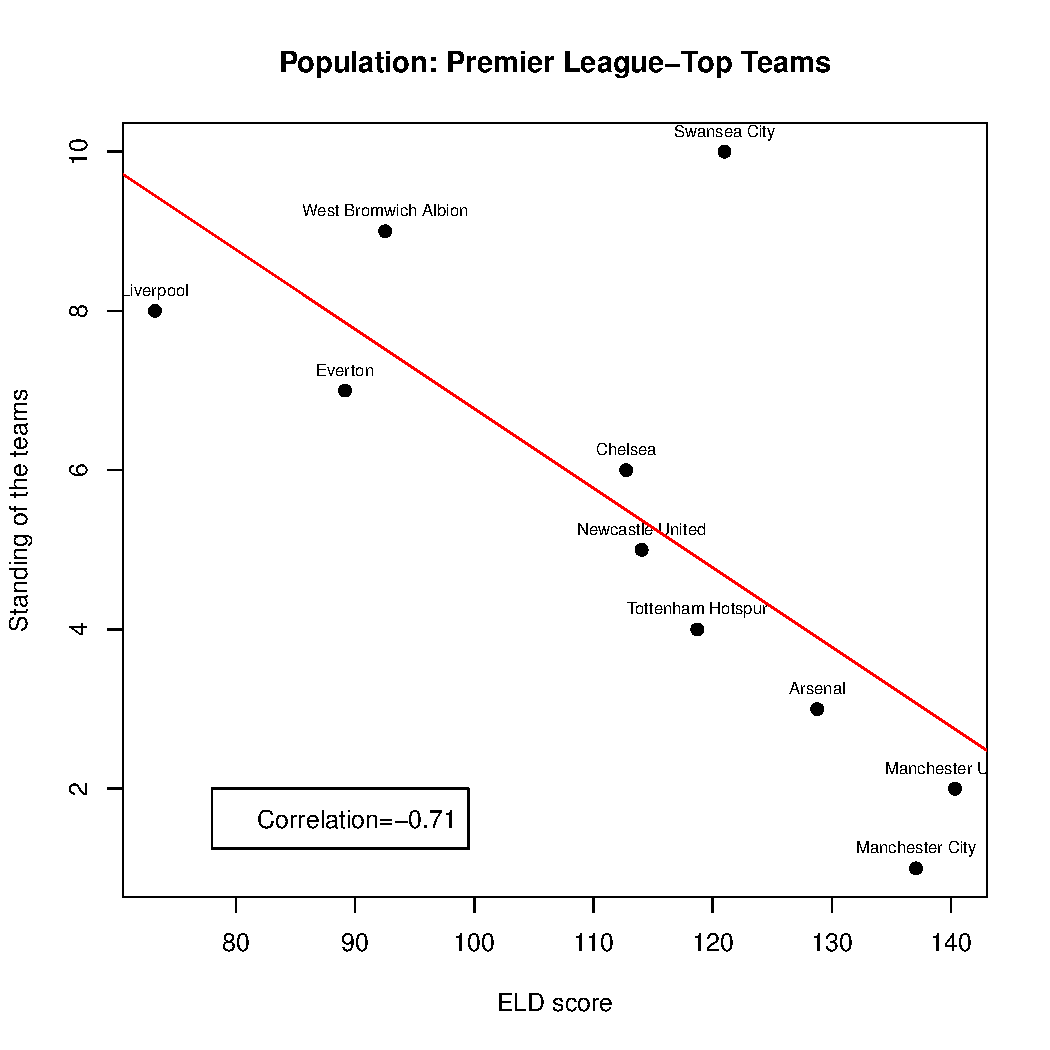
\includegraphics[width=0.8\textwidth]{topTeamStats-Sep.pdf}
	
	\caption{Teams: Team Standing vs. $\mid$ for the top teams in Premier League. 
		\label{fig:TeamStandingELD}}
\end{figure}

\subsubsection{Soccer Players}

	\paragraph{Players Time Played} is the total time that a player played over all matches in the season. This metric was shown to correlate strongly with other success metrics, such as salary, in soccer data~\cite{schwartz}. 
%	Tables ~\ref{table:goalie} and \ref{table:players} 
%	
%	and Figures \ref{fig:GoalieTime} and \ref{fig:StrikerTime} 
%	
%	show the correlation between the ELD metric and time played. 
	For each subgroup, there is a strong positive correlation with $\mid$, meaning that atypical players with higher $\mid$ tend to play more minutes.
	
	%The results are mixed; they show that pay cannot be adequately explained by past performance
%	alone, nor are pay levels justified by future performance. The bids for players in the initial
%	auction appear to have been based on intangibles that are hard to quantify%
	\paragraph{Salary} is probably the most obvious, and at the same time often the most misleading way to measure success of the players. Previous studies suggest that salary of the players does not  always follow their performance in many sports such as Baseball and Soccer~\cite{Hall2002,Barrio2004}. They show that pay cannot be explained only by past performance and there are other factors that are hard to quantify and have great effects on the salaries. 
	
	 We manually collected salaries of 120 players that we could find on-line. Table \ref{table:ELDwithPlayer}  and Figures~\ref{fig:strikersELD} and \ref{fig:goaliesELD} show the correlation between $\mid$ and this success metric. The correlation is high, especially for Strikers. We found salary data for only 5 goalies. We discuss the relatively weaker salary correlation for midfielders in more detail below.
	 
	 \paragraph{Shots on Target} applies to strikers only. This is defined as any shot attempt that would or does enter the goal if left unblocked. We record the total number of these shots over all matches of the strikers only. This metric was shown to correlate strongly with $\mid$ (see Table \ref{table:ELDwithPlayer}, Figure~\ref{fig:StrikerShot}).
	 
	 Figure~\ref{fig:strikersELD} plots $\mid$ against striker success metrics. We observe a large cluster around the origin, which points to a large base of normal strikers with both salaries and low $\mid$ scores. %The striker with the greatest $\mid$ score is Robin van Persie. He stands out in terms of Shots on Target, Time Played, and Salary. 
	 
	 %should probably label the points with individual names


	\begin{figure}
		\centering     %%% not \center
		\subfigure[Strikers: Salary vs $\mid$. ]{\label{fig:StrikerSalary}\includegraphics[width=0.65\textwidth]{1d-sumStrikerSalary.pdf}}
		\subfigure[Strikers: Shots On Target vs $\mid$]{\label{fig:StrikerShot}\includegraphics[width=0.65\textwidth]{1d-ShotsonTarget-sumStrikerStatistics.pdf}}
		\subfigure[Strikers: Time played vs $\mid$.]{\label{fig:StrikerTime}\includegraphics[width=0.65\textwidth]{1d-sumStrikerStatistics.pdf}}
		\caption{Correlations in Strikers population\label{fig:strikersELD}}
	\end{figure}


	 
	\paragraph{Saves Made} applies to Goalies only. It is defined as the total number of saves that goalies had made over all the matches. This metric shows a strong correlation with $\mid$ as well (see Table~\ref{table:ELDwithPlayer}, Figure\ref{fig:GoalieSaves}).  
	
	Figure~\ref{fig:goaliesELD} shows the correlation of $\mid$ with Goalie success metrics in a scatter plot. Goalies do not vary much in terms of the time they play. Wayne Hennessey has the highest number of Saves Made and also an unusually high $\mid$ score, although not the highest. 


	
	\begin{figure}
		\centering     %%% not \center
		\subfigure[Goalies: sum of time played vs $\mid$. ]{\label{fig:GoalieTime}\includegraphics[width=0.7\textwidth]{sumGoalieStatistics.pdf}}
		\subfigure[Goalies: sum of saves made vs $\mid$]{\label{fig:GoalieSaves}\includegraphics[width=0.7\textwidth]{sumGoalieStatisticsSavesMade.pdf}}
	%	\subfigure[Teams: Team Standing vs. $\mid$ for the top teams in Premier League. \textbf{separate figure please}]{\label{fig:TeamStanding}\includegraphics[width=0.5\textwidth]{topTeamStats.pdf}}
		\caption{\label{fig:goaliesELD}}
	\end{figure}


\paragraph{Midfielder Salary} 

We omit a scatterplot for midfielder salary vs. $\mid$ because it is less informative due to the weaker  correlation (0.45).
%
%While there is a strong correlation between salary of the Strikers and ELD score (0.79), this correlation becomes weaker in the Goalie population and even less apparent in Midfielder group. 
To investigate the reason for the weaker correlation, we picked two midfielders: 1) Stephane Sessegnon  who has been ranked second in the $\mid$ ranking but does not draw a large salary. 2) Steven Gerrard who is a very well known player and ranked second in the Salary ranking but according to the $\mid$ score, he has been ranked 21. Based on domain knowledge, we picked some of the features that are relevant to midfield performance from the raw data and compared the feature statistics for these two players. Table~\ref{table:MidfielderComparison} shows the details of their appearances in different matches. Sessegnon scored higher than Gerrard in three out of the four categories (passes and Time Played). However, his salary was much lower than Gerrard's. Indeed his next contract with West Bromwich Albion netted him a club record fee. This is an example of how our $\mid$ metric can identify players who are underpaid relative to their potential.
%This is an example of how weak the correlation is between salary and the observed box scores, which are the basis for the $\mid$ metric. 
%to show how unfair and unreliable the salary is in this domain.
%	 Unsuccessful Passes&Successful Long Passes
		\begin{table}[htbp]
			
			\centering
			\resizebox{1\textwidth}{!}{
				\begin{tabular}{|l|l|c|c|c|c|c|c|c|}
					\hline
					Name&Team&age&\begin{tabular}{c}Salary\\Ranking \end{tabular}&\begin{tabular}{c}$\mid$\\Ranking \end{tabular}&\begin{tabular}{c}Time\\Played \end{tabular}&\begin{tabular}{c}Unsuccessful\\Passes \end{tabular}&\begin{tabular}{c}Successful\\Long Passes \end{tabular}&\begin{tabular}{c}Successful\\corners \end{tabular}\\\hline
					Steven Gerrard	&Liverpool&31&2&21&1212 min&244&52&25\\\hline
					Stephane Sessegnon&Sunderland&26&22&2&3133 min&231&82&15\\\hline
					
					%	$\mid$&0.71&0.73&0.6\\\hline
				\end{tabular}}
				%
				\caption{Comparison of two midfielders.\label{table:MidfielderComparison}}
			\end{table}

	
	
						
						\begin{table}
						
						
							\centering
							\resizebox{1\textwidth}{!}{
								\begin{tabular}{|c|c|c|c|c|c|}
									\hline
									Class&Time On Ice &Power Play Time&Assists&Goals\\\hline
									Forwarder&0.79&0.78&0.81&0.78\\\hline
									Defender&0.66&0.57&0.60&0.40\\\hline
									
									%Synthetic&40&280\\ \hline
								\end{tabular}}
									\caption{Correlation between $\mid$ metric and success metrics of NHL Players.	\label{table:ELDwithHockey}}
							\end{table}
	\subsubsection{Hockey Players}
	For the hockey players the features that we have selected as success metrics are as follows: $\it{Time on Ice}$, that can be defined as the total amount of time a player has played over the course of a season. $\it{Power Play Time}$ which is the total amount of power player time for a given player in a season. $\it{Assists}$ is the total number of any actions that led to a goal. And finally total number of $\it{Goals}$ that a given player has scored.
The correlation between these features and $\mid$ is shown in Table~\ref{table:ELDwithHockey}. ELD has high correlations in features of both categories, however, it is stronger in Forwarder subgroup.
		\paragraph{Movie Sum of Ratings}
	\subsubsection{Movies} 
	
	\paragraph{Movie Sum of Ratings} is the number of user ratings of a movie. Table~\ref{table:ELDmovie} shows a high correlation with the $\mid$ metric. The highest correlation obtains for the genre Comedy (0.84). 
	%See Figure~\ref{fig:ActionRate},Figure~\ref{fig:ComedyRate}, Figure~\ref{fig:DramaRate}). 
	The correlation between a movie and the sum of its ratings is equally strong, but the correlation with its average rating is much weaker. Thus the $\mid$ score is related mainly with how many users have rated the movie rather than with how they have rated it. The number of ratings is a meaningful success metric as it indicates the number of people who have gone to see a movie.  
	

%\textcolor{red}{need to fix cross-reference} Figure~\ref{fig:Movies} shows the correlation of $\mid$ with movie success metrics in a scatter plot. We again observe a large cluster of movies around the origin. For drama and comedy movies, the top rated movies are (``American Beauty'' resp. ``Being John Malkovich''); these also stand out in the $\mid$ metric. 


%	\begin{figure}
%		\centering     %%% not \center
%		\subfigure[Action movies: sum of ratings by users vs $\mid$. ]{\label{fig:ActionRate}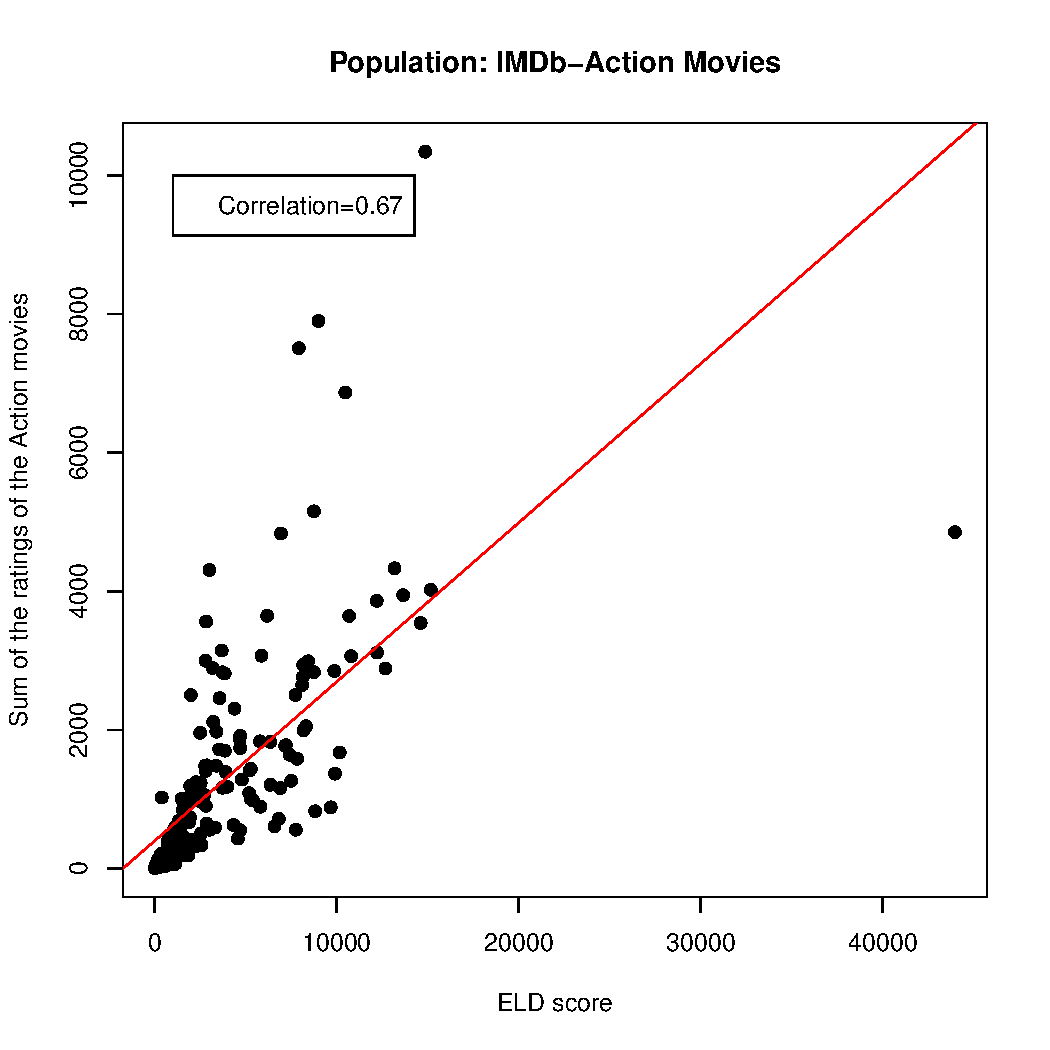
\includegraphics[width=0.48\textwidth]{NewPlotsJan2016/Action-Correlation.pdf}}
%		\subfigure[Comedy movies: sum of ratings by users vs $\mid$]{\label{fig:ComedyRate}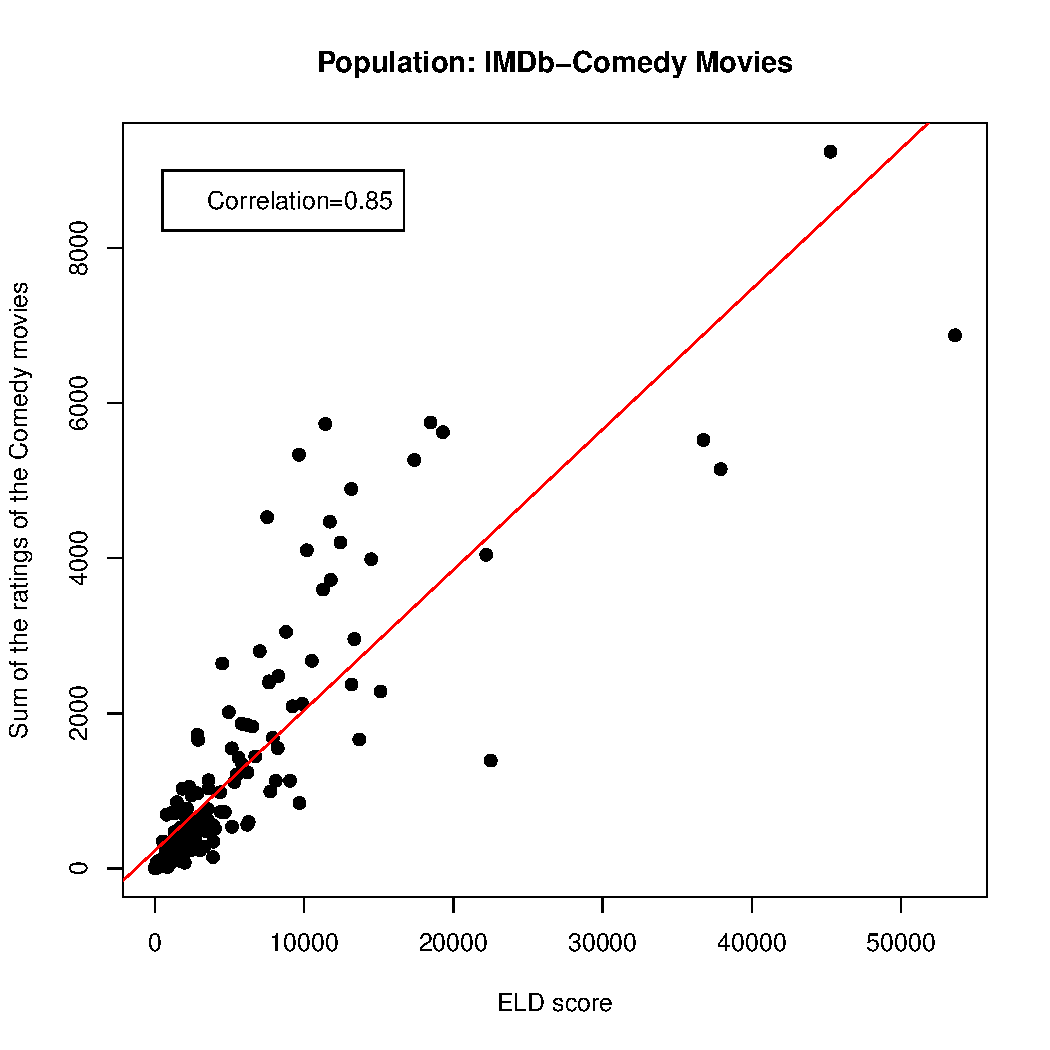
\includegraphics[width=0.5\textwidth]{NewPlotsJan2016/Comedy-Correlation.pdf}}
%		\subfigure[Drama movies: sum of ratings by users vs $\mid$.]{\label{fig:DramaRate}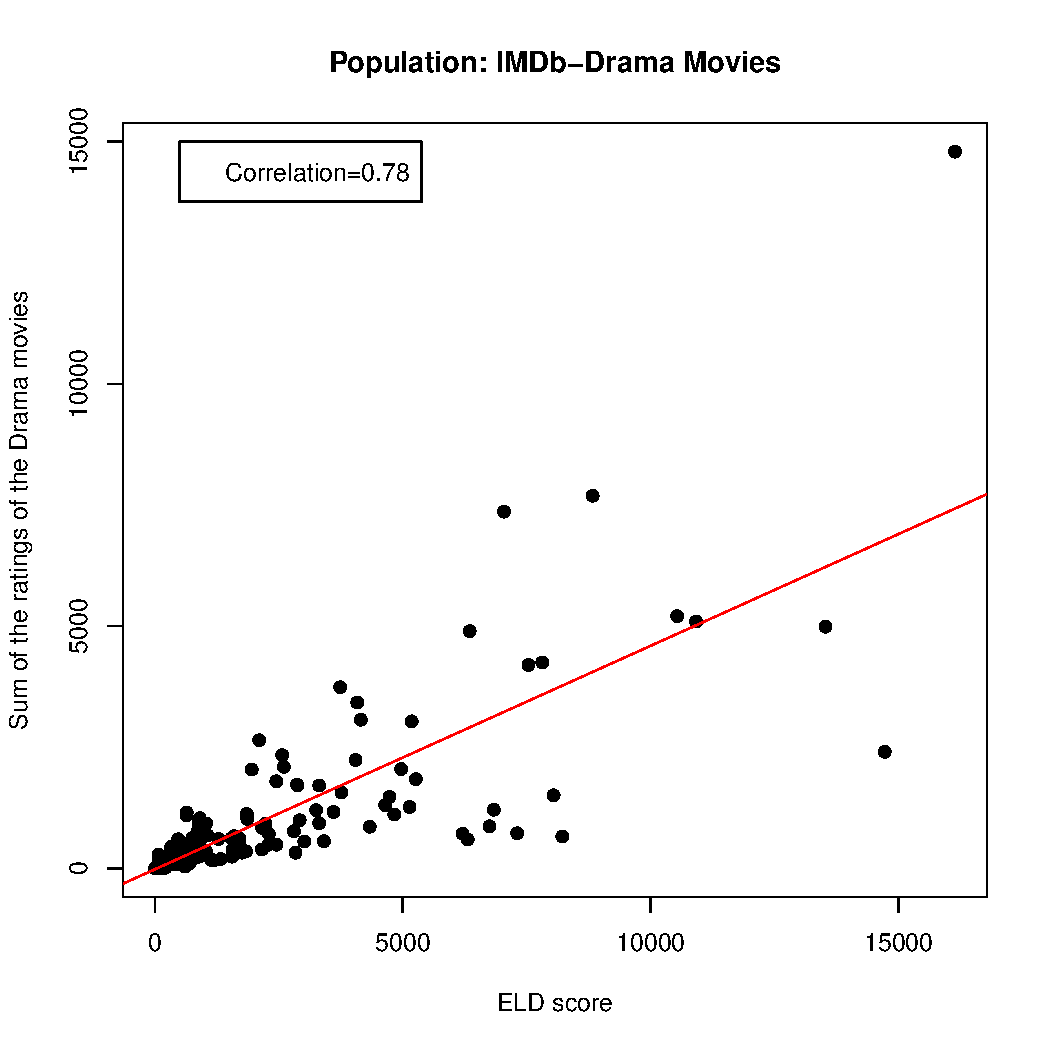
\includegraphics[width=0.5\textwidth]{NewPlotsJan2016/Drama-Correlation.pdf}}
%		\caption{\label{fig:Movies}}
%	\end{figure}


\subsection{Correlations between other outlier metrics and success} \label{sec:corr-others}
In Section~\ref{sec:log} and~\ref{sec:metrics} we introduced other metrics that could be used in order to detect outliers. In this section we discuss the correlation between those metrics and success. The correlation between $\mid$ and success is always stronger than $\textit{FD}$ and $\textit{LR}$ in all the datasets and subgroups, therefore we omit those results. The Log-likelihood is the only metric that results in a stronger correlation in some datasets and subgroups. Table~\ref{table:correlationLOGELD} shows the subgroups that Log-likelihood has a stronger correlation than the $\mid$ metric. 
In a way a high correlation with success can be interpreted as detecting in-class outliers and this results shows that Log-likelihood could be an alternative score to detect those type of outliers.
		\begin{table}

			\centering
			\resizebox{1\textwidth}{!}{
				\begin{tabular}{|l|l|c|c|}
					\hline
					Subgroup&Success metric&$\mid$ correlation&Log-likelihood correlation\\\hline
					Comedy&Sum of Rating&0.85&0.87\\\hline
					Drama&Sum of Rating&0.78&0.82\\\hline
					PL-Midfielder&Pass Efficiency&0.77&0.89\\\hline
					PL-Midfielder&Time Played&0.80&0.86\\\hline
					PL-Goalies&Time Played&0.77&0.87\\\hline
					PL-Goalies&Saves Made&0.74&0.85\\\hline
					NHL-Forward&Time on Ice&0.79&0.95\\\hline
					NHL-Forward&Goals&0.78&0.83\\\hline
		
					
				\end{tabular}
			}			\caption{Subgroups and success metrics for which the log-likelihood metric's correlates with success stronger than $\mid$.\label{table:correlationLOGELD}}
		\end{table}

\section{Conclusion and Future Work} We presented a new approach for applying Bayesian networks to object-relational outlier detection, a challenging and practically important topic for machine learning. The key idea is to apply the Exceptional Model Mining framework as follows. First, use statistical-relational learning to construct from relational data a graphical model. Then learn one set of parameter values that represent class-level associations, another set to represent object-level associations, and compare how well each parametrization fits the relational data that characterize the target object. The classic metric for comparing two parametrized models is their likelihood ratio. As an novel alternative, we  define  a new relational log-likelihood distance metric via two transformations:  (1) a mutual information decomposition, and (2) replacing log-likelihood differences by log-likelihood distances. This metric combines a single feature component, where features are treated as independent, with a correlation component that measures the deviation in the features' mutual information.

In experiments on three synthetic and four real-world outlier sets, the EMM methods based on likelihood ratio and the log-likelihood distance achieved the best detection accuracy. On all but one real-world dataset, log-likelihood distance outperformed the likelihood ratio. As an alternative to model-based EMM, converting the structured data to a flat data matrix via aggregation had a negative impact on outlier detection. 
Case studies showed that the EMM scores lead to easily interpreted rankings. We found that the log-distance score correlated with success metrics to a surprising degree, across different domains and classes of individuals. The correlation with metrics of independent interest corroborates that the log-distance score produces meaningful and interesting results.
%
%Overall, our new log-likelihood distance metric provides a promising new approach for applying machine learning techniques to outlier detection for object-relational data, a challenging and practically important topic. 

 							
There are several avenues for future work.  (i) A limitation of our current approach is that it ranks potential outliers, but does not set a threshold for a binary identification of outlier vs. non-outlier. (ii) Our divergence uses expected L1-distance for interpretability, but other distance scores like L2 could be investigated as well. (iii) Extending the expected L1-distance for continuous features is a useful addition. (iv) Compare our metric with the interestingness measures that have been developed for relational exception mining. (v) In the movie and soccer domains, our metric identified exceptionally successful individual objects, but not exceptionally unsuccessful ones. Our hypothesis was that in these domains, individuals have gone through a rigorous selection process, so the normal baseline performance is high. While we provided evidence for this hypothesis, it can be further investigated,  by applying our outlier detection to datasets that feature a range of skills, rather than professional performance. (vi) The theoretical properties of our $\mid$ metric are important to understand. For example, when is the Taylor series approximation of $\mid$ by Total Variation Distance sufficient close that theoretical guarantees for TVD hold also for $\mid$
%, and may facilitate combining our object-oriented approach with dimensional hierarchies in an OLAP data cube.
								%Distribution distances other than KLD could be evaluated for outlier detection (e.g., variation distance). However, the KLD variants have special advantages: their asymetry reflects the asymetry between object and class. Also, in a Bayesian network representation of the joint distributions, they decompose into a node-wise sum for easy computation and interpretation. 
								%A promising project for future work would be to combine the object data model and the multi-dimensional model to combine our object outlier method with OLAP-based methods. For example, one could add numeric measures and aggregate attributes to the object model. Another view: convert the object-oriented data to OLAP data, then use their outlier detection.
								
								
In sum, outlier metrics based on model likelihoods are a new type of structured outlier score for object-relational data.  Our evaluation indicates that  model-based scores provide informative, interpretable, and accurate rankings of objects as potential outliers. 
								
\section*{Acknowledgements} This work was supported by a Discovery Grant from the Natural Sciences and Engineering Research Council of Canada. We are indebted for helpful discussions to the participants at the 2018 Workshop on Statistical Relational AI. The action editor and reviewers for the Data Mining and Knowledge Discovery Journal provided extensive helpful comments. We thank Peter Flach for clarifying the connection with Exceptional Model Mining.

\section{Appendix: Proofs} \label{sec:proofs}
%For the ELD generator $f=-ln(u)$, we have $f'(1)=1$, so the first-order approximation to ELD is exactly TVD. 

{\em 
Assume that the generator $f$ is twice differentiable for $f$-divergence $I_{f}$. Then $I_{f}(P_{1}||P_{2}) \approx \frac{f''(1)}{2} \chi^{2}(P_{1}||P_{2}) = \frac{f''(1)}{2} 
\sum_{i=1}^{m}  \frac{(P_{2}(\nodevalue_{i})-P_{1}(\nodevalue_{i}))^{2}}
 {P_{1}(\nodevalue_{i})}$. 
}
\begin{proof}

Truncating the Taylor series for $f$ at $i=2$, the $f$-divergence expression~\ref{eq:f-divergence} becomes 

\begin{eqnarray*}
& & \sum_{i=1}^{m} P_{1}(\nodevalue_{i}) [f'(1) \left(\frac{P_{2}(\nodevalue_{i})}{P_{1}(\nodevalue_{i})}-1\right) + \frac{f''(1)}{2} \left(\frac{P_{2}(\nodevalue_{i})}{P_{1}(\nodevalue_{i})}-1\right)^{2}]  \\
& = &\sum_{i=1}^{m} P_{1}(\nodevalue_{i}) [f'(1) \left(\frac{P_{2}(\nodevalue_{i})-P_{1}(\nodevalue_{i})}{P_{1}(\nodevalue_{i})}\right) + \frac{f''(1)}{2} \left(\frac{P_{2}(\nodevalue_{i})-P_{1}(\nodevalue_{i})}{P_{1}(\nodevalue_{i})}\right)^{2}] \\
 & = & f'(1) [\sum_{i=1}^{m} P_{2}(\nodevalue_{i}) - \sum_{i=1}^{m} P_{1}(\nodevalue_{i})] + \sum_{i=1}^{m} \frac{f''(1)}{2} 
 \frac{(P_{2}(\nodevalue_{i})-P_{1}(\nodevalue_{i}))^{2}}
 {P_{1}(\nodevalue_{i})} \\
& = &   0 + \frac{f''(1)}{2} \chi^{2}(P_{1}||P_{2})
\end{eqnarray*}

\end{proof}

{\em The first-order Taylor series approximation for $\mid$ is total variation distance:
$$\mid(P_{1}||P_{2}) \approx  \TVD. $$}

\begin{proof}
Truncating the Taylor series for $f=-\ln(u)$ at $i=1$, the $|f|$-divergence expression~\ref{eq:f-absolute} becomes 

\begin{eqnarray}
& & \sum_{i:f(\frac{P_{2}(\nodevalue_{i})}{P_{1}(\nodevalue_{i})})>0} P_{1}(\nodevalue_{i}) f'(1) \left(\frac{P_{2}(\nodevalue_{i})}{P_{1}(\nodevalue_{i})}-1\right) -  \sum_{i:f(\frac{P_{2}(\nodevalue_{i})}{P_{1}(\nodevalue_{i})})<0} P_{1}(\nodevalue_{i}) f'(1) \left(\frac{P_{2}(\nodevalue_{i})}{P_{1}(\nodevalue_{i})}-1\right) \notag \\
& = &\sum_{i:f(\frac{P_{2}(\nodevalue_{i})}{P_{1}(\nodevalue_{i})})>0} P_{1}(\nodevalue_{i}) f'(1) \left(\frac{P_{2}(\nodevalue_{i})-P_{1}(\nodevalue_{i})}{P_{1}(\nodevalue_{i})}\right) - \sum_{i:f(\frac{P_{2}(\nodevalue_{i})}{P_{1}(\nodevalue_{i})})<0} P_{1}(\nodevalue_{i}) f'(1) \left(\frac{P_{2}(\nodevalue_{i})-P_{1}(\nodevalue_{i})}{P_{1}(\nodevalue_{i})}\right) \notag \\
 & = & 
- \sum_{i:P_{2}(\nodevalue_{i})<P_{1}(\nodevalue_{i})}
P_{2}(\nodevalue_{i})-P_{1}(\nodevalue_{i}) + \sum_{i:P_{2}(\nodevalue_{i})>P_{1}(\nodevalue_{i})}
 P_{2}(\nodevalue_{i})-P_{1}(\nodevalue_{i}) \label{eq:f-specific}
 \\
& = &   \sum_{i} |P_{2}(\nodevalue_{i})-P_{1}(\nodevalue_{i}) | \notag
\end{eqnarray}
Equation~\eqref{eq:f-specific} holds for $f = -\ln$ because then $f(\frac{P_{2}(\nodevalue_{i})}{P_{1}(\nodevalue_{i})})>0$ if and only if $P_{2}(\nodevalue_{i}) < P_{1}(\nodevalue_{i})$ and also $f'(1) = -1$.
\end{proof}




%\subsection{Discussion and ScatterPlots} 
%
%We now discuss the observed correlations in detail, according to different groups of individuals. To aid the discussion we provide scatter plots with best line of fit.
%
%
%
%\subsubsection{Striker Success}
%


%\begin{figure} \label{fig:strikers}
%		\centering
%		\begin{minipage}{0.45\linewidth}
%			\centering
%			\includegraphics[width=2.5in]{NewPlotsJan2016/1d-sumStrikerSalary.pdf}
%			\caption{Strikers: Salary vs ELD. \textbf{How many strikers?}}
%			\label{fig:StrikerSalary}
%		\end{minipage}
%		\hspace{0.05\linewidth}
%		\begin{minipage}{0.45\linewidth}
%			\centering
%			\includegraphics[width=2.5in]{NewPlotsJan2016/1d-ShotsonTarget-sumStrikerStatistics.pdf}
%			\caption{Strikers: Shots On Target vs ELD}
%			\label{fig:StrikerShot}
%		\end{minipage}
%		\hspace{0.05\linewidth}
%		\begin{minipage}{0.45\linewidth}
%			\centering
%			\includegraphics[width=2.5in]{NewPlotsJan2016/1d-sumStrikerStatistics.pdf}
%			\caption{Strikers: Time played vs ELD. \textbf{Why strikers only?}}
%			\label{fig:StrikerTime}
%		\end{minipage}
%	\end{figure}

% Non-BibTeX users please use
%\begin{thebibliography}{}
%%
%% and use \bibitem to create references. Consult the Instructions
%% for authors for reference list style.
%%
%\bibitem{RefJ}
%% Format for Journal Reference
%Author, Article title, Journal, Volume, page numbers (year)
%% Format for books
%\bibitem{RefB}
%Author, Book title, page numbers. Publisher, place (year)
%% etc
%\end{thebibliography}

%\subsubsection{Goalie Success} 





	


%\begin{figure} \label{fig:goalies}
%		\centering
%%		\begin{minipage}{0.45\linewidth}
%%			\centering
%%			\includegraphics[width=2.5in]{NewPlotsJan2016/topTeamStats.pdf}
%%			\caption{Teams: Correlation between team's Standing and ELD for the top teams in Premier League standing}
%%			\label{fig:teamStanding}
%%		\end{minipage}
%%		\hspace{0.05\linewidth}
%		\begin{minipage}{0.45\linewidth}
%			\centering
%			\includegraphics[width=2.5in]{NewPlotsJan2016/sumGoalieStatistics.pdf}
%			\caption{Goalies: sum of time played vs ELD}
%			\label{fig:GoalieTime}
%		\end{minipage}
%		\hspace{0.05\linewidth}
%		\begin{minipage}{0.45\linewidth}
%			\centering
%			\includegraphics[width=2.5in]{NewPlotsJan2016/sumGoalieStatisticsSavesMade.pdf}
%			\caption{Goalies: sum of saves made vs ELD}
%			\label{fig:GoalieSaves}
%		\end{minipage}
%	\end{figure}



%
%Figure~\ref{fig:teamStanding} shows the scatter plot of this correlation and its best fit regression line.

%\begin{figure} \label{fig:teamStanding}
%		\centering
%		\begin{minipage}{0.45\linewidth}
%			\centering
%			\includegraphics[width=2.5in]{NewPlotsJan2016/topTeamStats.pdf}
%			\caption{Teams: Correlation between team's Standing and ELD for the top teams in Premier League standing}
%			\label{fig:teamStanding}
%		\end{minipage}
%	\end{figure}


%\subsubsection{Movie Success} 




%\begin{figure} \label{fig:Movies}
%		\centering
%		\begin{minipage}{0.465\linewidth}
%			\centering
%			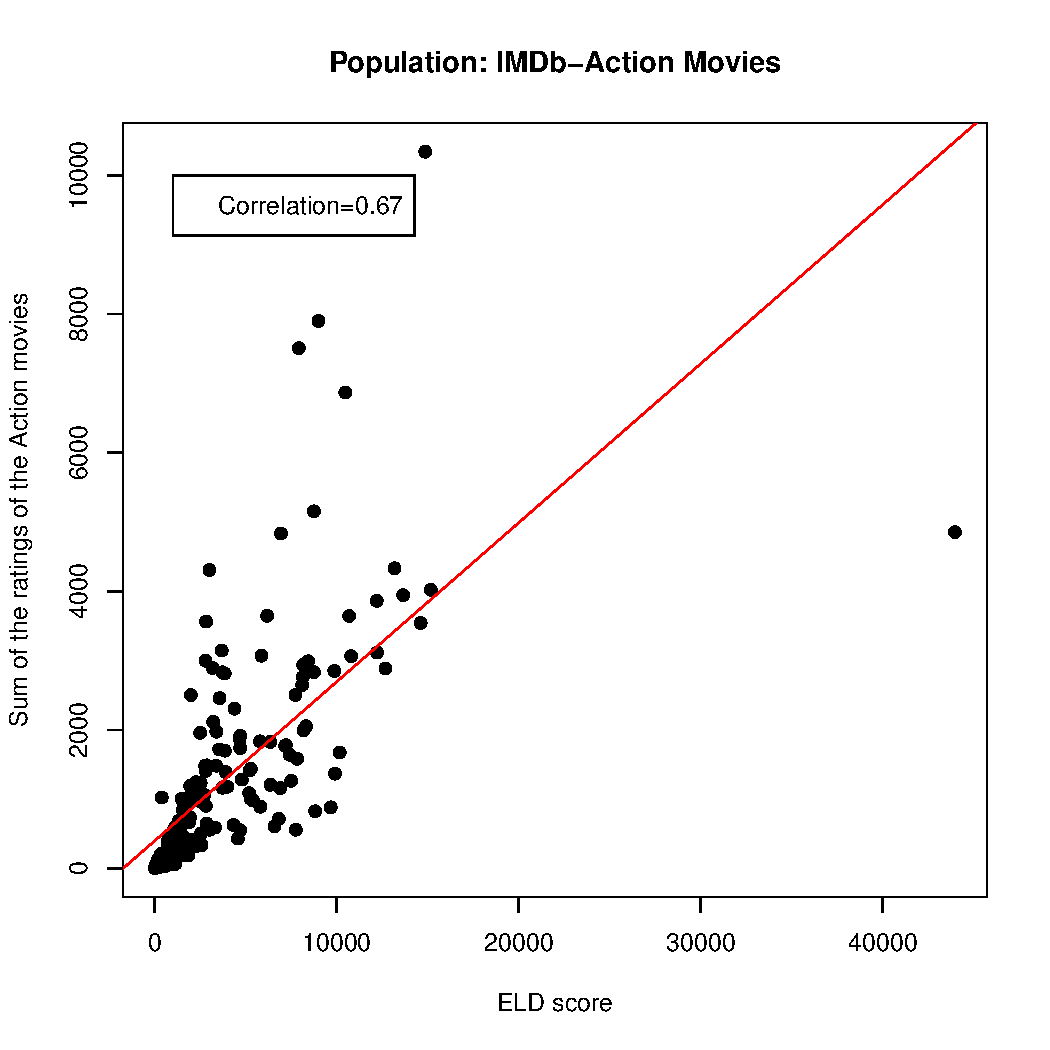
\includegraphics[width=2.5in]{NewPlotsJan2016/Action-Correlation.pdf}
%			\caption{Action movies: sum of ratings by users vs ELD}
%			\label{fig:ActionRate}
%		\end{minipage}
%		\hspace{0.05\linewidth}
%		\begin{minipage}{0.465\linewidth}
%			\centering
%			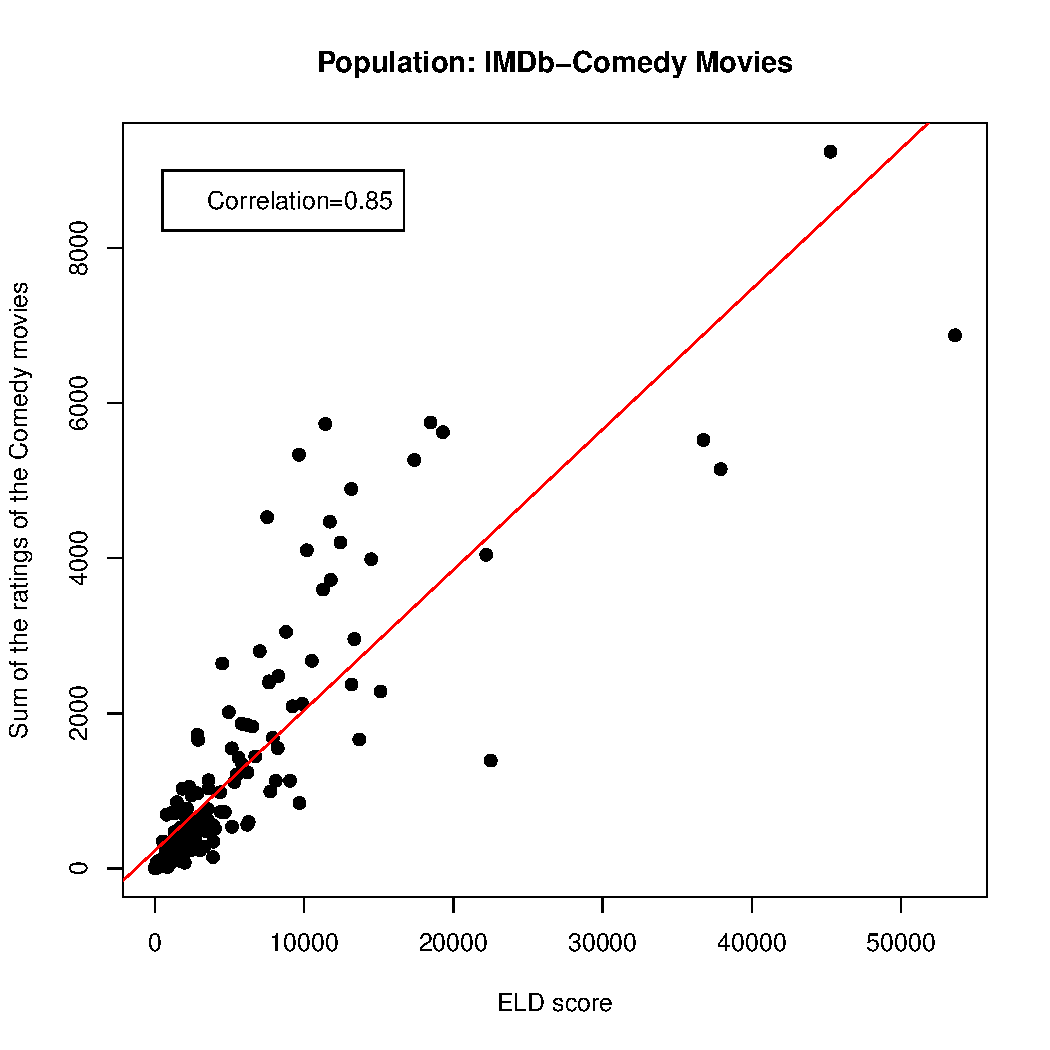
\includegraphics[width=2.5in]{NewPlotsJan2016/Comedy-Correlation.pdf}
%			\caption{Comedy movies: sum of ratings by users vs ELD}
%			\label{fig:ComedyRate}
%		\end{minipage}
%		\hspace{0.05\linewidth}
%		\begin{minipage}{0.465\linewidth}
%			\centering
%			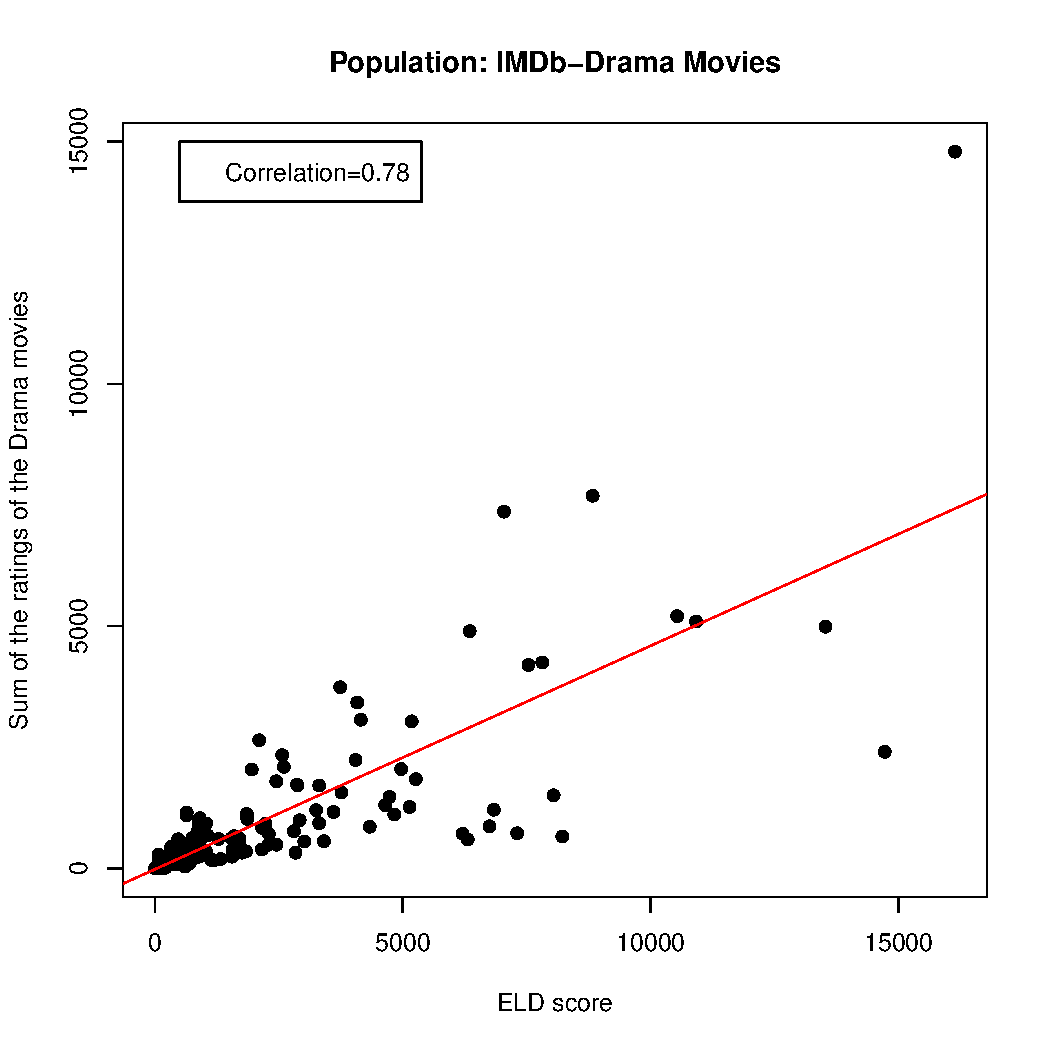
\includegraphics[width=2.5in]{NewPlotsJan2016/Drama-Correlation.pdf}
%			\caption{Drama movies: sum of ratings by users vs ELD \textbf{Average Rating?}}
%			\label{fig:DramaRate}
%		\end{minipage}
%	\end{figure}
%	
\
bibliographystyle{abbrv}
\begin{filecontents*}{jobname.bib}
	% This file was created with JabRef 2.7.
	% Encoding: ISO8859_1
	
	@INPROCEEDINGS{Riedel2013,
		author = {Sebastian Riedel and Limin Yao and Andrew McCallum and Benjamin M.
			Marlin},
		title = {Relation Extraction with Matrix Factorization and Universal Schemas},
		booktitle = {Human Language Technologies: NAA},
		year = {2013},
		pages = {74--84},
		bibsource = {dblp computer science bibliography, http://dblp.org},
		biburl = {http://dblp.uni-trier.de/rec/bib/conf/naacl/RiedelYMM13},
		timestamp = {Fri, 21 Feb 2014 14:03:41 +0100},
		url = {http://aclweb.org/anthology/N/N13/N13-1008.pdf}
	}
	
	
	@INPROCEEDINGS{Riahi2015,
		author = {Fatemeh Riahi and Oliver Schulte},
		title = {Model-based Outlier Detection for Object-Relational Data},
		booktitle = {IEEE Symposium Series on Computational Intelligence (SSCI},
		year = {2015},
		owner = {oschulte},
		timestamp = {2015.12.14}
	}
	
	
	@inproceedings{schulte2014aggregating,
		title={Aggregating predictions vs. aggregating features for relational classification},
		author={Schulte, Oliver and Routley, Kurt},
		booktitle={Computational Intelligence and Data Mining (CIDM), 2014 IEEE Symposium on},
		pages={121--128},
		year={2014},
		organization={IEEE}
	}
	@inproceedings{Akoglu2010,
		author = {Akoglu, Leman and McGlohon, Mary and Faloutsos, Christos},
		title = {OddBall: Spotting Anomalies in Weighted Graphs},
		booktitle = {Proceedings of the 14th Pacific-Asia Conference on Advances in Knowledge Discovery and Data Mining - Volume Part II},
		series = {PAKDD'10},
		year = {2010},
		isbn = {3-642-13671-0, 978-3-642-13671-9},
		location = {Hyderabad, India},
		pages = {410--421},
		numpages = {12},
		url = {http://dx.doi.org/10.1007/978-3-642-13672-6_40},
		doi = {10.1007/978-3-642-13672-6_40},
		acmid = {2144081},
		publisher = {Springer-Verlag},
		address = {Berlin, Heidelberg},
	} 
	@article{Akoglu2015,
		author = {Akoglu, Leman and Tong, Hanghang and Koutra, Danai},
		title = {Graph Based Anomaly Detection and Description: A Survey},
		journal = {Data Min. Knowl. Discov.},
		volume = {29},
		number = {3},
		month = may,
		year = {2015},
		acmid = {2757629},
		publisher = {Kluwer Academic Publishers},
		address = {Hingham, MA, USA},
		keywords = {Anomaly description, Anomaly detection, Change point detection, Event detection, Fraud detection, Graph mining, Network anomaly detection, Visual analytics},
	} 
	
	@article{Horvath2001,
		author="Horv{\'a}th, Tam{\'a}s
		and Wrobel, Stefan
		and Bohnebeck, Uta",
		title="Relational Instance-Based Learning with Lists and Terms",
		journal="Machine Learning",
		year="2001",
		volume="43",
		number="1",
		pages="53--80",
		issn="1573-0565"
	}
	
	@inproceedings{Khot2014,
		author = {Khot, Tushar and Natarajan, Sriraam and Shavlik, Jude},
		title = {Relational One-class Classification: A Non-parametric Approach},
		booktitle = {Proceedings of the Twenty-Eighth AAAI Conference on Artificial Intelligence},
		series = {AAAI'14},
		year = {2014},
		location = {Qu\&\#233;bec City, Qu\&\#233;bec, Canada},
		pages = {2453--2459},
		numpages = {7},
		url = {http://dl.acm.org/citation.cfm?id=2892753.2892892},
		acmid = {2892892},
		publisher = {AAAI Press},
	} 
	
	@inproceedings{AndersonP08,
		author    = {Grant Anderson and
			Bernhard Pfahringer},
		title     = {Exploiting Propositionalization Based on Random Relational Rules for
			Semi-supervised Learning},
		booktitle = {Advances in Knowledge Discovery and Data Mining, 12th Pacific-Asia
			Conference, {PAKDD} 2008, Osaka, Japan, May 20-23, 2008 Proceedings},
		pages     = {494--502},
		year      = {2008},
		crossref  = {DBLP:conf/pakdd/2008},
		url       = {http://dx.doi.org/10.1007/978-3-540-68125-0_43},
		doi       = {10.1007/978-3-540-68125-0_43},
		timestamp = {Thu, 15 May 2008 13:29:54 +0200}
	}
	@INPROCEEDINGS{kuzelka2008,
		author = {Ondvrej Kuvzelka and Filip Zelezny},
		title = {HiFi: Tractable Propositionalization through Hierarchical Feature
			Construction},
		booktitle = {Late Breaking Papers, ILP},
		year = {2008},
		category = {ida-publications}
	}
	
	@INPROCEEDINGS{Riahi2016,
		author = {Fatemeh Riahi, Oliver Schulte},
		title = {Propositionalization for Unsupervised Outlier	Detection in Multi-Relational Data},
		booktitle = {The Florida Association of Artificial Intelligence},
		year = {2016}
	}
	@inproceedings{Lavrac13,
		author = {Perovsek, Matic and Vavpetic, Anze and Cestnik, Bojan and Lavrac, Nada},
		booktitle = {Discovery Science},
		crossref = {conf/dis/2013},
		keywords = {dblp},
		publisher = {Springer},
		series = {Lecture Notes in Computer Science},
		title = {A Wordification Approach to Relational Data Mining.},
		year = 2013
	}
	@Inbook{Horvath1999,
		author="Horv{\'a}th, Tam{\'a}s
		and Alexin, Zolt{\'a}n
		and Gyim{\'o}thy, Tibor
		and Wrobel, Stefan",
		editor="D{\v{z}}eroski, Sa{\v{s}}o
		and Flach, Peter",
		title="Application of Different Learning Methods to Hungarian Part-of-Speech Tagging",
		bookTitle="Inductive Logic Programming: 9th International Workshop, ILP-99 Bled, Slovenia, June 24--27, 1999 Proceedings",
		year="1999",
		publisher="Springer Berlin Heidelberg",
		address="Berlin, Heidelberg",
		pages="128--139"
	}
	@Inbook{Kirsten2001,
		author="Kirsten, Mathias
		and Wrobel, Stefan
		and Horv{\'a}th, Tam{\'a}s",
		editor="D{\v{z}}eroski, Sa{\v{s}}o
		and Lavra{\v{c}}, Nada",
		title="Distance Based Approaches to Relational Learning and Clustering",
		bookTitle="Relational Data Mining",
		year="2001",
		publisher="Springer Berlin Heidelberg",
		address="Berlin, Heidelberg",
		pages="213--232
	}
	
	
	@INCOLLECTION{Cussen2007,
		author = {James Cussens},
		title = {Logic-based Formalisms for Statistical Relational Learning},
		booktitle = {Introduction to Statistical Relational Learning},
		publisher = {MIT Press},
		year = {2007},
		crossref = {SRL2007},
		owner = {hkhosrav},
		timestamp = {2008.10.10}
	}
	@ARTICLE{McHale2011,
		title = {A Bradley-Terry type model for forecasting tennis match results},
		author = {McHale, Ian and Morton, Alex},
		year = {2011},
		journal = {International Journal of Forecasting},
		volume = {27},
		number = {2},
		pages = {619-630},
	}
	
	@TechReport{Barrio2004,
		author={Pedro Garcia-del-Barrio and Francesc Pujol},
		title={{Pay and Performance in the Spanish Soccer League: Who Gets the Expected Monopsony Rents?}},
		year=2004,
		month=Mar,
		institution={School of Economics and Business Administration, University of Navarra},
		type={Faculty Working Papers},
		url={https://ideas.repec.org/p/una/unccee/wp0504.html},
		number={05/04}
	}
	
	@article{Hall2002,
		author = {Hall, Stephen and Szymanski, Stefan and Zimbalist, Andrew S.}, 
		title = {Testing Causality Between Team Performance and Payroll: The Cases of Major League Baseball and English Soccer},
		volume = {3}, 
		number = {2}, 
		pages = {149-168}, 
		year = {2002}, 
		URL = {http://jse.sagepub.com/content/3/2/149.abstract}, 
		eprint = {http://jse.sagepub.com/content/3/2/149.full.pdf+html}, 
		journal = {Journal of Sports Economics} 
	}
	@article{McHale2012,
		author = {McHale, Ian G. and Scarf, Philip A. and Folker, David E.},
		title = {On the Development of a Soccer Player Performance Rating System for the English Premier League},
		journal = {Interfaces},
		issue_date = {July-August 2012},
		volume = {42},
		number = {4},
		month = jul,
		year = {2012},
		issn = {0092-2102},
		pages = {339--351},
		numpages = {13},
		url = {http://dx.doi.org/10.1287/inte.1110.0589},
		doi = {10.1287/inte.1110.0589},
		acmid = {2344718},
		publisher = {INFORMS},
		address = {Institute for Operations Research and the Management Sciences (INFORMS), Linthicum, Maryland, USA},
		keywords = {football, performance measurement, ranking, sports and recreation},
	} 
	@BOOK{McHale2007,
		title = {  Statistical  analysis  of  the  FIFA	world rankings},
		publisher = {Statistical Thinking in Sport, Chapman and Hall},
		year = {2007},
		author = {McHale, Ian and Morton, Alex},
		abstract = {url = {http://researchbooks.org/1598296922}}
	}
	@BOOK{Keri2006,
		title = {Baseball Between the Numbers},
		publisher = {Basic Book},
		year = {2006},
		author = {Jonah Keri, James Click}
	}
	@BOOK{Goldman2010,
		title = {Baseball Prospectus 2010: The Essential Guide to the 2010 Baseball Season},
		publisher = {John  Wiley  \&  Sons,  Inc.,Hoboken},
		year = {2010},
		author = {Steven Goldman,Christina Kahrl }
	}
	
	@INCOLLECTION{Cussens2007,
		author = {James Cussens},
		title = {Logic-based Formalisms for Statistical Relational Learning},
		booktitle = {Introduction to Statistical Relational Learning},
		publisher = {MIT Press},
		year = {2007},
		crossref = {SRL2007},
		owner = {hkhosrav},
		timestamp = {2008.10.10}
	}
	@BOOK{PAPASTERGIADIS2013,
		title = {Futebol and Myths of the Brazilian Way of Life},
		publisher = { Cultural Studies Review},
		year = {2013},
		author = {Nikos,PAPASTERGIADIS},
		abstract = {url = {http://researchbooks.org/1598296922}}
	}
	@ARTICLE{Wooten2013,
		author = {Jadrian James Wooten },
		title = {Can Ranking Nationalities Explain the Salary Discrepancies in Major League Soccer},
		journal = {Social Science Research Network},
		year = {2013}
	}
	@INCOLLECTION{bib:jensen-chapter,
		author = {Jennifer Neville and David Jensen},
		title = {Relational Dependency Networks},
		booktitle = {Introduction to Statistical Relational Learning},
		publisher = {MIT Press},
		year = {2007},
		chapter = {8},
		pages = {239-268},
		crossref = {SRL2007},
		owner = {oschulte},
		timestamp = {2008.11.24}
	}
	
	@INPROCEEDINGS{Kriegel2007,
		author = {Achtert, Elke and Bohm, Christian and Kriegel, Hans-Peter and Kroger,
			Peer and Muller-Gorman, Ina and Zimek, Arthur},
		title = {Detection and Visualization of Subspace Cluster Hierarchies.},
		booktitle = {DASFAA},
		year = {2007},
		publisher = {Springer},
		description = {dblp},
		keywords = {dblp}
	}
	
	@INPROCEEDINGS{Elke2013,
		author = {Elke Achtert and Hans{-}Peter Kriegel and Erich Schubert and Arthur
			Zimek},
		title = {Interactive data mining with 3D-parallel coordinate trees},
		booktitle = {Proceedings of the 2013 ACM SIGMOD},
		year = {2013},
		bibsource = {dblp computer science bibliography, http://dblp.org},
		biburl = {http://dblp.uni-trier.de/rec/bib/conf/sigmod/AchtertKSZ13},
		doi = {10.1145/2463676.2463696},
		timestamp = {Wed, 26 Jun 2013 09:37:17 +0200},
		
		address = {New York, NY, USA},
		url = {http://doi.acm.org/10.1145/2463676.2463696}
	}
	
	@BOOK{aggarwal2013,
		title = {Outlier Analysis},
		publisher = {Springer New York},
		year = {2013},
		author = {Aggarwal, C.C.},
		isbn = {9781461463955},
		lccn = {2012956186},
		url = {http://books.google.ca/books?id=900CkgEACAAJ}
	}
	
	@INPROCEEDINGS{cussens2012,
		author = {Alsanie, Waleed and Cussens, James },
		title = {Learning Recursive PRISM Programs with Observed Outcomes},
		booktitle = {Proceedings of the ICML-2012 Workshop on Statistical-Relational Learning},
		year = {2012}
	}
	
	@ARTICLE{Angiulli2007,
		author = {Angiulli, Fabrizio and Greco, Gianluigi and Palopoli, Luigi},
		title = {Outlier Detection by Logic Programming},
		journal = {ACM Transactions on Computer Logic},
		year = {2004},
		journal = {CoRR},
		keywords = {dblp},
		reasoning},
	publisher = {ACM}
}

@INPROCEEDINGS{Babbar2010,
	author = {Babbar, Sakshi and Chawla, Sanjay},
	title = {On Bayesian Network and Outlier Detection.},
	booktitle = {COMAD},
	year = {2010},
	editor = {Kumar, P. Sreenivasa and Parthasarathy, Srinivasan and Godbole, Shantanu},
	pages = {125},
	publisher = {Allied Publishers},
	added-at = {2012-07-20T00:00:00.000+0200},
	biburl = {http://www.bibsonomy.org/bibtex/2e12ea37af712f96b331c00d466b2530e/dblp},
	ee = {http://www.cse.iitb.ac.in/~comad/2010/ResearchTrack/paper%2017.pdf},
		file = {:/local-scratch/SRiahi/Desktop/texmf/Babbar2010.pdf:PDF},
		interhash = {8f627abe7d2f74667ae6ddd6e72dd970},
		intrahash = {e12ea37af712f96b331c00d466b2530e},
		keywords = {dblp},
		timestamp = {2012-07-20T00:00:00.000+0200},
		url = {http://dblp.uni-trier.de/db/conf/comad/comad2010.html#BabbarC10}
	}
	
	@ARTICLE{RePEc:taf:japsta,
		author = {Baio, Gianluca and Blangiardo, Marta},
		title = {Bayesian hierarchical model for the prediction of football results},
		journal = {Journal of Applied Statistics},
		year = {2010},
		volume = {37},
		pages = {253-264},
		number = {2}
	}
	
	@INPROCEEDINGS{Balog,
		author = {Balog, Krisztian and Bogers, Toine and Azzopardi, Leif and de Rijke,
			Maarten and van den Bosch, Antal},
		title = {Broad expertise retrieval in sparse data environments},
		year = {2007},
		series = {SIGIR '07},
		pages = {551--558},
		address = {New York, NY, USA},
		publisher = {ACM}
	}
	
	@INPROCEEDINGS{foil,
		author = {Joseph Bockhorst and Irene Ong},
		title = {FOIL-D: Efficiently scaling FOIL for multi-relational data mining
			of large datasets},
		booktitle = {In Proceedings of the 14th international},
		year = {2004},
		pages = {63--79}
	}
	
	@INPROCEEDINGS{Breunig2000,
		author = {Markus Breunig and Hans-Peter Kriegel and Raymond T. Ng and Jörg
			Sander},
		title = {LOF: Identifying Density-Based Local Outliers},
		booktitle = { Proceedings of ACM SIGMOD},
		year = {2000}
	}
	
	@ARTICLE{Cansado2008,
		author = {Cansado, Antonio and Soto, Alvaro},
		title = {UNSUPERVISED ANOMALY DETECTION IN LARGE DATABASES USING {Bayes Nets}},
		journal = {Appllied Artificial Intelligence},
		year = {2008},
		acmid = {1451348},
		address = {Bristol, PA, USA},
		doi = {10.1080/08839510801972801},
		issn = {0883-9514},
		issue_date = { 2008},
		numpages = {22},
		publisher = {Taylor \& Francis, Inc.}
	}
	
	@ARTICLE{CaoJYPLHH12,
		author = {Liangliang Cao and Xin Jin and Zhijun Yin and Andrey Del Pozo and
			Jiebo Luo and Jiawei Han and Thomas S. Huang},
		title = {RankCompete: Simultaneous ranking and clustering of information networks},
		journal = {Neurocomputing},
		year = {2012},
		volume = {95},
		pages = {98-104},
		bibsource = {DBLP, http://dblp.uni-trier.de},
		ee = {http://dx.doi.org/10.1016/j.neucom.2011.06.038}
	}
	
	@ARTICLE{Chan2004,
		author = {Chan, Antoni B and Vasconcelos, Nuno and Moreno, Pedro J},
		title = {A family of probabilistic kernels based on information divergence},
		journal = {Tech. Rep. SVCL-TR},
		year = {2004}
	}
	
	@ARTICLE{han2009,
		author = {Chen, Hailiang and Liu, Hongyan and Han, Jiawei and Yin, Xiaoxin},
		title = {Exploring Optimization of Semantic Relationship Graph for Multi-relational
			{B}ayesian Classification},
		journal = {Decision Support Systems},
		year = {2009},
		volume = {48},
		pages = {112-121},
		number = {1}
	}
	
	@ARTICLE{Chiang2012,
		author = {Michael Chiang and David Poole},
		title = {Reference classes and relational learning},
		journal = {Int. J. Approx. Reasoning},
		year = {2012},
		volume = {53},
		pages = {326-346},
		number = {3},
		bibsource = {DBLP, http://dblp.uni-trier.de},
		ee = {http://dx.doi.org/10.1016/j.ijar.2011.05.002},
		file = {Chiang2012.pdf:Chiang2012.pdf:PDF}
	}
	
	@INPROCEEDINGS{Demartini,
		author = {Demartini, Gianluca and Gaugaz, Julien and Nejdl, Wolfgang},
		title = {A Vector Space Model for Ranking Entities and Its Application to
			Expert Search},
		booktitle = {31st European Conference on IR Research on Advances in Information
			Retrieval},
		year = {2009},
		series = {ECIR '09},
		pages = {189--201},
		address = {Berlin, Heidelberg},
		publisher = {Springer-Verlag},
		location = {Toulouse, France}
	}
	
	@INPROCEEDINGS{Deng,
		author = {Hongbo Deng and Irwin King and Michael R. Lyu},
		title = {Formal models for expert finding on dblp bibliography data},
		booktitle = {In ICDM},
		year = {2008},
		pages = {163--172}
	}
	
	@INCOLLECTION{bib:query-ex,
		author = {L. Deshape and H. Toivonen},
		title = {Discovery of Relational Association Rules},
		booktitle = {Relational Data Mining},
		publisher = {Springer, Berlin},
		year = {2001},
		editor = {Saso Dzeroski and Nada Lavrac},
		chapter = {8},
		owner = {oliverschulte},
		review = {warmr},
		timestamp = {2008.10.29}
	}
	
	@BOOK{Domingos2009,
		title = {Markov Logic: An Interface Layer for Artificial Intelligence},
		publisher = {Morgan and Claypool Publishers},
		year = {2009},
		author = {Pedro Domingos and Daniel Lowd},
		abstract = {url = {http://researchbooks.org/1598296922}}
	}
	
	@MISC{url,
		author = {Fatemeh Riahi and Oliver Schulte},
		title = {{Codes and Datasets. [Online].  Available:}},
		howpublished = {\url{ftp://ftp.fas.sfu.ca/pub/cs/oschulte/CodesAndDatasets/}},
		year = {2015}
	}
	
	@ARTICLE{Fawcett2006,
		author = {Fawcett, Tom},
		title = {An Introduction to {ROC} Analysis},
		journal = {Pattern Recogn. Lett.},
		year = {2006},
		address = {New York, NY, USA},
		issue_date = { 2006},
		keywords = {Classifier evaluation, Evaluation metrics, ROC analysis},
		publisher = {Elsevier Science Inc.}
	}
	
	@ARTICLE{Fisher1921,
		author = {Fisher, R. A.},
		title = {{On the probable error of a coefficient of correlation deduced from
				a small sample}},
		journal = {Metron},
		year = {1921},
		volume = {1},
		pages = {3--32},
		keywords = {methods}
	}
	
	@INPROCEEDINGS{Friedman1998,
		author = {Nir Friedman and Moises Goldszmidt},
		title = {Learning {B}ayesian networks with local structure},
		booktitle = {NATO ASI on Learning in graphical models},
		year = {1998},
		pages = {421--459},
		file = {Friedman1998.pdf:Friedman1998.pdf:PDF},
		keywords = {digging, {B}ayes Nets},
		owner = {hkhosrav},
		timestamp = {2008.10.08}
	}
	
	@ARTICLE{Campos2006,
		author = {L. de Campos},
		title = {A scoring function for learning {B}ayes nets based on mutual information
			and conditional independence tests},
		journal = {Journal of Machine learning Research },
		year = {2006},
		owner = {hkhosrav},
		timestamp = {2008.10.08}
	}
	@INPROCEEDINGS{Gao2010,
		author = {Gao, J. and Liang, F. and Fan, W. and Wang, Y. and Han, J.},
		title = {On Community Outliers and Their Detection in Information Network},
		booktitle = {Proceedings of ACM SIGKDD},
		year = {2010},
		numpages = {10}
	}
	
	@BOOK{SRL2007,
		title = {Introduction to statistical relational learning},
		publisher = {MIT Press},
		year = {2007},
		author = {Lise Getoor and Ben Taskar},
		owner = {hkhosrav},
		timestamp = {2008.10.08}
	}
	
	@ARTICLE{griffiths,
		author = {Griffiths, T. L. and Steyvers, M.},
		title = {Finding scientific topics},
		journal = {Proceedings of the National Academy of Sciences},
		year = {2004},
		volume = {101},
		pages = {5228-5235},
		month = {April},
		keywords = {gibbs lda models sampling topic}
	}
	
	@ARTICLE{Guo2005,
		author = {Guo, Hong and Jack, L. B. and Nandi, Asoke K.},
		title = {Feature generation using genetic programming with application to
			fault classification.},
		journal = {IEEE Transactions on Systems, Man, and Cybernetics, Part B},
		year = {2005},
		volume = {35},
		pages = {89-99},
		number = {1},
		date = {2006-08-23}
	}
	
	@INPROCEEDINGS{Gupta2013a,
		author = {Gupta, Manish and Gao, Jing and Yan, Xifeng and Cam, Hasan and Han,
			Jiawei},
		title = {On detecting association-based clique outliers in heterogeneous info.
			net.},
		booktitle = {ASONAM},
		year = {2013},
		publisher = {ACM}
	}
	
	@INPROCEEDINGS{2002-gyftodimos,
		author = {Elias Gyftodimos and Peter Flach},
		title = {Hierarchical Bayesian Networks: A Probabilistic Reasoning Model for
			Structured Domains},
		booktitle = ICML-2002 # Workshop # on # Development # of # Representations
	}
	
	@INPROCEEDINGS{Hill2007,
		author = {David J. Hill and Barbara S. Minsker and Eyal Amir},
		title = {Real-time bayesian anomaly detection for environmental sensor data},
		booktitle = {In 32nd Conference of IAHR, the International Association of Hydraulic
			Engineering \& Research},
		year = {2007},
		file = {:/local-scratch/SRiahi/Desktop/texmf/Hill2007.pdf:PDF}
	}
	
	@ARTICLE{Hodge2004,
		author = {Hodge, Victoria and Austin, Jim},
		title = {A Survey of Outlier Detection Methodologies},
		journal = {Artif. Intell. Rev.},
		year = {2004},
		acmid = {1028946},
		address = {Norwell, MA, USA},
		doi = {10.1023/B:AIRE.0000045502.10941.a9},
		file = {:/local-scratch/SRiahi/Desktop/texmf/Hodge2004.pdf:PDF},
		issn = {0269-2821},
		issue_date = {October 2004},
		keywords = {anomaly, detection, deviation, noise, novelty, outlier, recognition},
		numpages = {42},
		owner = {oschulte},
		publisher = {Kluwer Academic Publishers},
		timestamp = {2014.02.03},
		url = {http://dx.doi.org/10.1023/B:AIRE.0000045502.10941.a9}
	}
	
	@INPROCEEDINGS{Hulgeri,
		author = {Hulgeri, Arvind and Nakhe, Charuta},
		title = {Keyword Searching and Browsing in Databases using BANKS},
		booktitle = {Proceedings of the 18th International Conference on Data Engineering},
		year = {2002},
		series = {ICDE},
		pages = {431--},
		address = {Washington, DC, USA},
		publisher = {IEEE Computer Society}
	}
	
	@MISC{IMDBoriginal,
		author = {{Internet Movie Database}},
		title = {Internet Movie Database},
		note = {[Online]. Available: URL = \url{http://www.imdb.com/}},
		owner = {oliverschulte},
		timestamp = {2009.10.02}
	}
	
	@MISC{InternetMovieDatabase,
		author = {{Internet Movie Database}},
		title = {Internet Movie Database},
		note = {URL = \url{http://www.imdb.com/}},
		owner = {oliverschulte},
		timestamp = {2009.10.02}
	}
	
	@INPROCEEDINGS{DavidJensen2002,
		author = {David Jensen and Jennifer Neville},
		title = {Linkage and autocorrelation cause feature selection bias in relational
			learning (2002)},
		booktitle = {ICML},
		year = {2002},
		file = {:D\:\\Hassan\\Subversion related\\references\\jensen1.pdf:PDF},
		owner = {hkhosrav},
		timestamp = {2008.10.08}
	}
	
	@ARTICLE{Joseph,
		author = {Joseph, A. and Fenton, N. E. and Neil, M.},
		title = {Predicting football results using Bayesian nets and other machine
			learning techniques},
		journal = {Know.-Based Syst.},
		year = {2006},
		volume = {19},
		pages = {544--553},
		number = {7},
		month = nov,
		issn = {0950-7051},
		issue_date = {November, 2006},
		numpages = {10},
		publisher = {Elsevier Science Publishers B. V.}
	}
	
	@MISC{bib:jbnsite,
		author = {H. Khosravi and T. Man and J. Hu and E. Gao and O. Schulte},
		title = {Learn and Join Algorithm Code.   },
		howpublished = {[Online]. Available: URL = \url{http://www.cs.sfu.ca/~oschulte/jbn/}},
		keywords = {statistical-relational},
		owner = {oliverschulte},
		timestamp = {2009.10.02}
	}
	
	@ARTICLE{Kleinberg,
		author = {Kleinberg, Jon M.},
		title = {Authoritative sources in a hyperlinked environment},
		journal = {J. ACM},
		year = {1999},
		volume = {46},
		pages = {604--632},
		number = {5},
		month = sep,
		address = {New York, NY, USA},
		numpages = {29},
		publisher = {ACM}
	}
	
	@INPROCEEDINGS{koh2008,
		author = {Koh, Judice LY and Lee, Mong Li and Hsu, Wynne and Ang, Wee Tiong},
		title = {Correlation-based attribute outlier detection in {XML}},
		booktitle = {Proceedings of ICDE. IEEE 24th},
		year = {2008}
	}
	
	@INPROCEEDINGS{Kriegel2009,
		author = {Kriegel, Hans-Peter and Kroger, Peer and Schubert, Erich and Zimek,
			Arthur},
		title = {Outlier Detection in Axis-Parallel Subspaces of High Dimensional
			Data.},
		booktitle = {PAKDD},
		year = {2009},
		publisher = {Springer},
		date = {2009-04-25},
		description = {dblp},
		keywords = {dblp},
		timestamp = {2009-04-25T00:00:00.000+0200}
	}
	
	@ARTICLE{Lunn,
		author = {Lunn, David J. and Thomas, Andrew and Best, Nicky and Spiegelhalter,
			David},
		title = {WinBUGS: Bayesian modelling framework: Concepts, structure, and extensibility},
		journal = {Statistics and Computing},
		year = {2000},
		volume = {10},
		pages = {325--337},
		number = {4},
		month = oct,
		issn = {0960-3174},
		issue_date = {October 2000},
		numpages = {13}
	}
	
	@ARTICLE{Maervoet2012,
		author = {Maervoet, Joris and Vens, Celine and Vanden Berghe, Greet and Blockeel,
			Hendrik and De Causmaecker, Patrick},
		title = {Outlier Detection in Relational Data: A Case Study},
		journal = {Expert System Applications},
		year = {2012},
		numpages = {11}
	}
	
	@OTHER{Doe:2009:Online,
		author = {ManchesterCity},
		month = jun,
		title = {URL:http://www.mcfc.com/},
		url = {http://www.mcfc.com/},
		year = {2012}
	}
	
	@MISC{opta-original,
		author = {{MCFC Analytics}},
		title = {The Premier League Dataset},
		note = {[Online]. Available: URL = \url{http://www.mcfc.co.uk/Home/MCFCAnalytics}},
		owner = {oliverschulte}
	}
	
	@ARTICLE{Mu2010,
		author = {Mu, Tingting and Pataky, Todd C. and Findlow, Andrew H. and Aung,
			Min S. H. and Goulermas, John Yannis},
		title = {Automated nonlinear feature generation and classification of foot
			pressure lesions.},
		journal = {IEEE Transactions on Information Technology in Biomedicine},
		year = {2010},
		volume = {14},
		pages = {418-424},
		number = {2}
	}
	
	@INPROCEEDINGS{Muller2009,
		author = {Muller, Emmanuel and Assent, Ira and Gunnemann, Stephan and Krieger,
			Ralph and Seidl, Thomas},
		title = {Fast Algorithms for Projected Clustering},
		booktitle = {Proceedings of ICDM},
		year = {2009},
		biburl = {http://www.bibsonomy.org/bibtex/25e02212edb472f5f6833f9919e373667/dblp},
		keywords = {dblp}
	}
	@INPROCEEDINGS{Koller1997,
		author = {Daphne Koller and Avi Pfeffer},
		title = {Object-Oriented {B}ayes Nets},
		booktitle = {Proceedings of UAI},
		year = {1997},
		bibsource = {DBLP, http://dblp.uni-trier.de},
		keywords = {{B}ayes Nets, statistical-relational},
		owner = {oschulte},
		review = {introduces object-oriented bayes nets, which were mentioned by Chris
			Meek and cited by David Poole as similar to BLNs/parametrized belief
			nets.},
		timestamp = {2009.08.19}
	}
	@INPROCEEDINGS{Muller2012,
		author = {Muller, Emmanuel and Assent, Ira and Iglesias, Patricia and Mulle,
			Yvonne and Bohm, Klemens},
		title = {Outlier Ranking via Subspace Analysis in Multiple Views of the Data},
		booktitle = {Proceedings of ICDM},
		year = {2012},
		keywords = {outlier ranking, multiple subspaces, clusterings}
	}
	
	@BOOK{Neapolitan2004,
		title = {Learning {B}ayesian Networks},
		publisher = {Pearson Education},
		year = {2004},
		author = {R. E. Neapolitan},
		keywords = {digging},
		owner = {hkhosrav},
		timestamp = {2008.10.08}
	}
	
	@ARTICLE{Neyman1928,
		author = {Neyman, Jerzy and Pearson, E. S.},
		title = {On the Use and Interpretation of Certain Test Criteria for Purposes
			of Statistical Inference: Part I},
		journal = {Biometrika},
		year = {1928}
	}
	
	@INPROCEEDINGS{Nie,
		author = {Nie, Zaiqing and Zhang, Yuanzhi and Wen, Ji-Rong and Ma, Wei-Ying},
		title = {Object-level ranking: bringing order to Web objects},
		booktitle = {Proceedings of the 14th international conference on World Wide Web},
		year = {2005},
		pages = {567--574},
		address = {New York, NY, USA},
		publisher = {ACM},
		numpages = {8}
	}
	
	@ARTICLE{Novak2009,
		author = {Novak,Petra Kralj and Webb,Geoffrey I. and Wrobel,Stefan},
		title = {Supervised descriptive rule discovery: A unifying survey of contrast
			set, emerging pattern and subgroup mining},
		journal = {Journal of Machine Learning Research},
		year = {2009}
	}
	
	@ARTICLE{Onody:cond,
		author = {Roberto N. Onody and Paulo A. de Castro},
		title = {Complex network study of Brazilian soccer players},
		year = {2004}
	}
	@INPROCEEDINGS{Schulte2017a,
		author = {Oliver Schulte and Sajjad Gholami},
		title = {Locally Consistent {Bayesian} Network Scores for Multi-Relational
			Data},
		booktitle = {Proceedings of the International Joint Conference on Artificial Intelligence
			(IJCAI)},
		year = {2017},
		pages = {2693-2700},
		owner = {oschulte},
		timestamp = {2017.06.19},
		url = {\url{https://www.ijcai.org/proceedings/2017/0375.pdf}}
	}
	
	
	@TECHREPORT{ilprints422,
		author = {Lawrence Page and Sergey Brin and Rajeev Motwani and Terry Winograd},
		title = {The PageRank Citation Ranking: Bringing Order to the Web.},
		year = {1999},
		type = {Technical Report},
		number = {1999-66},
		month = {November},
		note = {Previous number = SIDL-WP-1999-0120},
		publisher = {Stanford InfoLab}
	}
	
	@BOOK{Pearl1988,
		title = {Probabilistic Reasoning in Intelligent Systems},
		publisher = {Morgan Kaufmann},
		year = {1988},
		author = {J. Pearl},
		keywords = {digging},
		owner = {hkhosrav},
		timestamp = {2008.10.08}
	}
	
	@TECHREPORT{Pei2006,
		author = {Yaling Pei and Osmar Zaiane},
		title = {A synthetic data generator for clustering and outlier analysis},
		year = {2006},
		file = {:local-scratch/SRiahi/texmf/Pei2006.pdf:PDF}
	}
	
	@TECHREPORT{Peralta2007,
		author = {Peralta, V.},
		title = {{Extraction and Integration of MovieLens and IMDb}},
		institution = {APDM project},
		year = {2007}
	}
	
	@INPROCEEDINGS{Poole2003,
		author = {David Poole},
		title = {First-order probabilistic inference},
		booktitle = {Proceedings of IJCAI},
		year = {2003},
		bibsource = {DBLP, http://dblp.uni-trier.de},
		file = {Poole2003.pdf:Poole2003.pdf:PDF},
		keywords = {{B}ayes Nets, statistical-relational}
	}
	
	@BOOK{Ramakrishnan2003,
		title = {Database Management Systems},
		publisher = {McGraw-Hill},
		year = {2003},
		author = {Raghu Ramakrishnan and Johannes Gehrke},
		edition = {3rd},
		owner = {oschulte},
		timestamp = {2012.06.08}
	}
	
	@ARTICLE{Ramaswamy2000,
		author = {Ramaswamy, Sridhar and Rastogi, Rajeev and Shim, Kyuseok},
		title = {Efficient Algorithms for Mining Outliers from Large Data Sets},
		journal = {SIGMOD},
		year = {2000},
		publisher = {ACM}
	}
	
	@INPROCEEDINGS{riahi2013,
		author = {Riahi, Fatemeh and Schulte, Oliver},
		title = {Identifying Important Nodes in Relational Data},
		booktitle = {AAAI Late Breaking Paper},
		year = {2013}
	}
	
	@BOOK{Russell2010,
		title = {Artificial Intelligence: A Modern Approach},
		publisher = {Prentice Hall},
		year = {2010},
		author = {Stuart Russell and Peter Norvig},
		owner = {oschulte},
		timestamp = {2011.09.30}
	}
	
	@INPROCEEDINGS{Sarawagi1998,
		author = {Sunita Sarawagi and Rakesh Agrawal and Nimrod Megiddo},
		title = {Discovery-driven Exploration of {OLAP} Data Cubes},
		booktitle = {Proceedings of International Conference on Extending Database Technology},
		year = {1998},
		publisher = {Springer-Verlag}
	}
	
	@INPROCEEDINGS{Schulte2011,
		author = {Oliver Schulte},
		title = {A tractable pseudo-likelihood function for {Bayes} Nets applied to
			relational data},
		booktitle = {Proceedings of SIAM SDM},
		year = {2011},
		keywords = {oliver, statistical-relational},
		owner = {oliverschulte},
		timestamp = {2011.01.13}
	}
	
	@ARTICLE{Schulte2012,
		author = {Oliver Schulte and Hassan Khosravi},
		title = {Learning graphical models for relational data via lattice search},
		journal = {Journal of Machine Learning},
		year = {2012},
		owner = {oliverschulte},
		timestamp = {2012.04.11}
	}
	
	@INPROCEEDINGS{Schulte2012b,
		author = {Oliver Schulte and Hassan Khosravi and Arthur Kirkpatrick and Tianxiang
			Gao and Yuke Zhu},
		title = {Modelling Relational Statistics With Bayes Nets},
		booktitle = {Inductive Logic Programming (ILP)},
		year = {2012},
		owner = {oschulte},
		timestamp = {2012.07.24}
	}
	
	@INPROCEEDINGS{schulte2013,
		author = {Schulte, Oliver and Riahi, Fatemeh and Li, Qing },
		title = {Identifying Important Nodes in Relational Data},
		booktitle = {AAAI Late Breaking Paper},
		year = {2013}
	}
	
	@MANUAL{RROCR2012,
		title = {ROCR: Visualizing the performance of scoring classifiers.},
		author = {Sing, Tobias and Sander, Oliver and Beerenwinkel, Niko and Lengauer,
			Thomas},
		year = {2012},
		note = {R package version 1.0-4},
		biburl = {http://www.bibsonomy.org/bibtex/2206b72ee617e5f5800c8836ae6d922d0/knutwenzig},
		interhash = {c0711b8f9d54e00acab614f43a077106},
		intrahash = {206b72ee617e5f5800c8836ae6d922d0},
		keywords = {MalteMasterThesis imported},
		timestamp = {2014-05-20T08:47:50.000+0200},
		url = {http://CRAN.R-project.org/package=ROCR}
	}
	
	@TECHREPORT{BUGS,
		author = {Spiegelhalter, D. and Thomas, A. and Best, N. and Gilks, W.},
		title = {BUGS: Bayesian inference using Gibbs sampling},
		institution = {Institute of Public Health},
		year = {1996},
		address = { Cambridge, UK},
		keywords = {Bayes,MCMC,npbayes}
	}
	
	@INPROCEEDINGS{Gupta2013,
		author = {Sun, Y. and Han, J. and Zhao, Peixiang and Yin, Zhijun and Cheng,
			Hong and Wu, Tianyi},
		title = {Community Distribution Outlier Detection in Heterogeneous network},
		booktitle = {ECML},
		year = {2013}
	}
	
	@INPROCEEDINGS{Sun2009,
		author = {Sun,Yizhou and Han Jiawei and Zhao,Peixiang },
		title = {RankClus: Integrating Clustering with Ranking for Heterogeneous Information
			Network Analysis},
		booktitle = {Proceedings of the International Conference on Extending Database
			Technology: Advances in Database Technology},
		year = {2009},
		pages = {565--576},
		address = {New York, NY, USA},
		publisher = {ACM},
		numpages = {12}
	}
	
	@ARTICLE{schwartz,
		author = {T.Swartz, Adriano Arce, Mohan Parameswaran},
		title = {Assessing Value of the Draft Positions in Major League Soccer's SuperDraft},
		journal = {The Sport Journal},
		year = {2013}
	}
	
	@CONFERENCE{Tang2013,
		author = {Guanting Tang and James Bailey and Jian Pei and Guozhu Dong},
		title = {Mining multidimensional contextual outliers from categorical relational
			data},
		booktitle = {Proceedings of SSDBM},
		year = {2013}
	}
	@INCOLLECTION{Kramer2000,
		author = {Kramer, Stefan and Lavrac, Nada and Flach, Peter},
		title = {Propositionalization approaches to relational data mining},
		booktitle = {Relational Data Mining},
		publisher = {Springer},
		year = {2000},
		book = {Relational Data Mining},
		comment = {Pages: 262-286},
		isbn = {3-540-42289-7}
	}
	
	@BOOK{Tuffery2011,
		title = {Data Mining and Statistics for Decision Making},
		publisher = {Wiley Series in Computational Statistics},
		year = {2011},
		author = {Stephane Tuffery},
		url = {http://ca.wiley.com/WileyCDA/WileyTitle/productCd-0470688297.html}
	}
	
	@INPROCEEDINGS{VazdeMelo,
		author = {Vaz de Melo, Pedro O.S. and Almeida, Virgilio A.F. and Loureiro,
			Antonio A.F.},
		title = {Can complex network metrics predict the behavior of NBA teams?},
		year = {2008},
		series = {KDD '08},
		pages = {695--703},
		publisher = {ACM},
		keywords = {complex networks, predictability, sports leagues},
		numpages = {9}
	}
	
	@ARTICLE{Vuong1989,
		author = {Vuong, Quang H.},
		title = {Likelihood Ratio Tests for Model Selection and Non-Nested Hypotheses},
		journal = {Econometrica},
		year = {1989},
		volume = {57},
		pages = {307-333},
		number = {2},
		copyright = {Copyright 1989 The Econometric Society},
		file = {Vuong1989.pdf:Vuong1989.pdf:PDF},
		issn = {00129682},
		jstor_articletype = {research-article},
		jstor_formatteddate = {Mar., 1989},
		language = {English},
		publisher = {The Econometric Society}
	}
	
	@BOOK{Witten2005,
		title = {Data Mining: Practical Machine Learning Tools and Techniques},
		publisher = {Morgan Kaufmann},
		year = {2005},
		author = {I. H. Witten and E. Frank}
	}
	
	@ARTICLE{Xu2010,
		author = {Xu, Jing and Shelton, Christian R.},
		title = {Intrusion Detection using Continuous Time Bayesian Networks.},
		journal = {J. Artif. Intell. Res. (JAIR)},
		year = {2010},
		volume = {39},
		pages = {745-774},
		added-at = {2011-01-09T00:00:00.000+0100},
		biburl = {http://www.bibsonomy.org/bibtex/2737d878a295499db478e8ff87b596d98/dblp},
		ee = {http://dx.doi.org/10.1613/jair.3050},
		file = {:/local-scratch/SRiahi/Desktop/texmf/Xu2010.pdf:PDF},
		interhash = {a43602fc202fe7b8b1438b3fec3f8080},
		intrahash = {737d878a295499db478e8ff87b596d98},
		keywords = {dblp},
		timestamp = {2011-01-09T00:00:00.000+0100},
		url = {http://dblp.uni-trier.de/db/journals/jair/jair39.html#XuS10}
	}
	
	@INPROCEEDINGS{Zhou,
		author = {Zhou, Ding and Orshanskiy, Sergey A. and Zha, Hongyuan and Giles,
			C. Lee},
		title = {Co-ranking Authors and Documents in a Heterogeneous Network},
		booktitle = {Proceedings of the 2007 Seventh IEEE International Conference on
			Data Mining},
		year = {2007},
		series = {ICDM '07},
		pages = {739--744},
		publisher = {IEEE Computer Society},
		acmid = {1442053},
		isbn = {0-7695-3018-4},
		numpages = {6}
	}
	
	@ARTICLE{Kimmig2014,
		author = {Kimmig, Angelika and Mihalkova, Lilyana and Getoor, Lise},
		title = {Lifted graphical models: a survey},
		journal = { Computing Research Repository},
		year = {2014},
		file = {:/Users/olivernew/Documents/svn-projects/punch-srl/texmf/Kimmig2014.pdf:PDF},
		publisher = {Springer}
	}
	@article{Akoglu2015,
		author = {Akoglu, Leman and Tong, Hanghang and Koutra, Danai},
		title = {Graph Based Anomaly Detection and Description: A Survey},
		journal = {Data Min. Knowl. Discov.},
		volume = {29},
		number = {3},
		month = may,
		year = {2015},
		acmid = {2757629},
		publisher = {Kluwer Academic Publishers},
		address = {Hingham, MA, USA},
		keywords = {Anomaly description, Anomaly detection, Change point detection, Event detection, Fraud detection, Graph mining, Network anomaly detection, Visual analytics}
	} 
	
	@INCOLLECTION{Heckerman+al:SRL07,
		author = {D. Heckerman and C. Meek and D. Koller},
		title = {Probabilistic Entity-Relationship Models, {PRMs}, and Plate Models},
		booktitle = {Introduction to Statistical Relational Learning},
		publisher = {MIT Press},
		year = {2007},
		editor = {L. Getoor and B. Taskar},
		crossref = {SRL2007},
		owner = {hkhosrav},
		timestamp = {2008.10.10}
	}
	@ARTICLE{Nickel2016,
		author = {Nickel, Maximilian and Murphy, Kevin and Tresp, Volker and Gabrilovich,
			Evgeniy},
		title = {A review of relational machine learning for knowledge graphs},
		journal = {Proceedings of the IEEE},
		year = {2016},
		volume = {104},
		pages = {11--33},
		number = {1},
		booktitle = {Proceedings of the I},
		publisher = {IEEE}
	}
	@PHDTHESIS{Getoor2001a,
		author = {Lise Getoor},
		title = {Learning Statistical Models From Relational Data},
		school = {Department of Computer Science, Stanford University},
		year = {2001},
		file = {Getoor2001a.pdf:Getoor2001a.pdf:PDF},
		owner = {oschulte},
		timestamp = {2010.03.02}
	}
	@ARTICLE{Schulte2014,
		author = {Oliver Schulte and Hassan Khosravi and Arthur Kirkpatrick and Tianxiang
			Gao and Yuke Zhu},
		title = {Modelling Relational Statistics With Bayes Nets},
		journal = {Machine Learning},
		year = {2014},
		volume = {94},
		pages = {105-125},
		owner = {zqian},
		timestamp = {2014.01.06},
		url = {http://link.springer.com/article/10.1007%2Fs10994-013-5362-7}
		}
		
	\end{filecontents*}
	\bibliographystyle{abbrv}
	\bibliography{jobname,master} 
\end{document}
\begin{filecontents*}{jobname.bib}
	% This file was created with JabRef 2.7.
	% Encoding: ISO8859_1
	
	@INPROCEEDINGS{Riedel2013,
		author = {Sebastian Riedel and Limin Yao and Andrew McCallum and Benjamin M.
			Marlin},
		title = {Relation Extraction with Matrix Factorization and Universal Schemas},
		booktitle = {Human Language Technologies: NAA},
		year = {2013},
		pages = {74--84},
		bibsource = {dblp computer science bibliography, http://dblp.org},
		biburl = {http://dblp.uni-trier.de/rec/bib/conf/naacl/RiedelYMM13},
		timestamp = {Fri, 21 Feb 2014 14:03:41 +0100},
		url = {http://aclweb.org/anthology/N/N13/N13-1008.pdf}
	}
	
	
	@INPROCEEDINGS{Riahi2015,
		author = {Fatemeh Riahi and Oliver Schulte},
		title = {Model-based Outlier Detection for Object-Relational Data},
		booktitle = {IEEE Symposium Series on Computational Intelligence (SSCI},
		year = {2015},
		owner = {oschulte},
		timestamp = {2015.12.14}
	}
	
	
	@inproceedings{schulte2014aggregating,
		title={Aggregating predictions vs. aggregating features for relational classification},
		author={Schulte, Oliver and Routley, Kurt},
		booktitle={Computational Intelligence and Data Mining (CIDM), 2014 IEEE Symposium on},
		pages={121--128},
		year={2014},
		organization={IEEE}
	}
	@inproceedings{Akoglu2010,
		author = {Akoglu, Leman and McGlohon, Mary and Faloutsos, Christos},
		title = {OddBall: Spotting Anomalies in Weighted Graphs},
		booktitle = {Proceedings of the 14th Pacific-Asia Conference on Advances in Knowledge Discovery and Data Mining - Volume Part II},
		series = {PAKDD'10},
		year = {2010},
		isbn = {3-642-13671-0, 978-3-642-13671-9},
		location = {Hyderabad, India},
		pages = {410--421},
		numpages = {12},
		url = {http://dx.doi.org/10.1007/978-3-642-13672-6_40},
		doi = {10.1007/978-3-642-13672-6_40},
		acmid = {2144081},
		publisher = {Springer-Verlag},
		address = {Berlin, Heidelberg},
	} 
	@article{Akoglu2015,
		author = {Akoglu, Leman and Tong, Hanghang and Koutra, Danai},
		title = {Graph Based Anomaly Detection and Description: A Survey},
		journal = {Data Min. Knowl. Discov.},
		volume = {29},
		number = {3},
		month = may,
		year = {2015},
		acmid = {2757629},
		publisher = {Kluwer Academic Publishers},
		address = {Hingham, MA, USA},
		keywords = {Anomaly description, Anomaly detection, Change point detection, Event detection, Fraud detection, Graph mining, Network anomaly detection, Visual analytics},
	} 
	
	@article{Horvath2001,
		author="Horv{\'a}th, Tam{\'a}s
		and Wrobel, Stefan
		and Bohnebeck, Uta",
		title="Relational Instance-Based Learning with Lists and Terms",
		journal="Machine Learning",
		year="2001",
		volume="43",
		number="1",
		pages="53--80",
		issn="1573-0565"
	}
	
	@inproceedings{Khot2014,
		author = {Khot, Tushar and Natarajan, Sriraam and Shavlik, Jude},
		title = {Relational One-class Classification: A Non-parametric Approach},
		booktitle = {Proceedings of the Twenty-Eighth AAAI Conference on Artificial Intelligence},
		series = {AAAI'14},
		year = {2014},
		location = {Qu\&\#233;bec City, Qu\&\#233;bec, Canada},
		pages = {2453--2459},
		numpages = {7},
		url = {http://dl.acm.org/citation.cfm?id=2892753.2892892},
		acmid = {2892892},
		publisher = {AAAI Press},
	} 
	
	@inproceedings{AndersonP08,
		author    = {Grant Anderson and
			Bernhard Pfahringer},
		title     = {Exploiting Propositionalization Based on Random Relational Rules for
			Semi-supervised Learning},
		booktitle = {Advances in Knowledge Discovery and Data Mining, 12th Pacific-Asia
			Conference, {PAKDD} 2008, Osaka, Japan, May 20-23, 2008 Proceedings},
		pages     = {494--502},
		year      = {2008},
		crossref  = {DBLP:conf/pakdd/2008},
		url       = {http://dx.doi.org/10.1007/978-3-540-68125-0_43},
		doi       = {10.1007/978-3-540-68125-0_43},
		timestamp = {Thu, 15 May 2008 13:29:54 +0200}
	}
	@INPROCEEDINGS{kuzelka2008,
		author = {Ondvrej Kuvzelka and Filip Zelezny},
		title = {HiFi: Tractable Propositionalization through Hierarchical Feature
			Construction},
		booktitle = {Late Breaking Papers, ILP},
		year = {2008},
		category = {ida-publications}
	}
	
	@INPROCEEDINGS{Riahi2016,
		author = {Fatemeh Riahi, Oliver Schulte},
		title = {Propositionalization for Unsupervised Outlier	Detection in Multi-Relational Data},
		booktitle = {The Florida Association of Artificial Intelligence},
		year = {2016}
	}
	@inproceedings{Lavrac13,
		author = {Perovsek, Matic and Vavpetic, Anze and Cestnik, Bojan and Lavrac, Nada},
		booktitle = {Discovery Science},
		crossref = {conf/dis/2013},
		keywords = {dblp},
		publisher = {Springer},
		series = {Lecture Notes in Computer Science},
		title = {A Wordification Approach to Relational Data Mining.},
		year = 2013
	}
	@Inbook{Horvath1999,
		author="Horv{\'a}th, Tam{\'a}s
		and Alexin, Zolt{\'a}n
		and Gyim{\'o}thy, Tibor
		and Wrobel, Stefan",
		editor="D{\v{z}}eroski, Sa{\v{s}}o
		and Flach, Peter",
		title="Application of Different Learning Methods to Hungarian Part-of-Speech Tagging",
		bookTitle="Inductive Logic Programming: 9th International Workshop, ILP-99 Bled, Slovenia, June 24--27, 1999 Proceedings",
		year="1999",
		publisher="Springer Berlin Heidelberg",
		address="Berlin, Heidelberg",
		pages="128--139"
	}
	@Inbook{Kirsten2001,
		author="Kirsten, Mathias
		and Wrobel, Stefan
		and Horv{\'a}th, Tam{\'a}s",
		editor="D{\v{z}}eroski, Sa{\v{s}}o
		and Lavra{\v{c}}, Nada",
		title="Distance Based Approaches to Relational Learning and Clustering",
		bookTitle="Relational Data Mining",
		year="2001",
		publisher="Springer Berlin Heidelberg",
		address="Berlin, Heidelberg",
		pages="213--232
	}
	
	
	@INCOLLECTION{Cussen2007,
		author = {James Cussens},
		title = {Logic-based Formalisms for Statistical Relational Learning},
		booktitle = {Introduction to Statistical Relational Learning},
		publisher = {MIT Press},
		year = {2007},
		crossref = {SRL2007},
		owner = {hkhosrav},
		timestamp = {2008.10.10}
	}
	@ARTICLE{McHale2011,
		title = {A Bradley-Terry type model for forecasting tennis match results},
		author = {McHale, Ian and Morton, Alex},
		year = {2011},
		journal = {International Journal of Forecasting},
		volume = {27},
		number = {2},
		pages = {619-630},
	}
	
	@TechReport{Barrio2004,
		author={Pedro Garcia-del-Barrio and Francesc Pujol},
		title={{Pay and Performance in the Spanish Soccer League: Who Gets the Expected Monopsony Rents?}},
		year=2004,
		month=Mar,
		institution={School of Economics and Business Administration, University of Navarra},
		type={Faculty Working Papers},
		url={https://ideas.repec.org/p/una/unccee/wp0504.html},
		number={05/04}
	}
	
	@article{Hall2002,
		author = {Hall, Stephen and Szymanski, Stefan and Zimbalist, Andrew S.}, 
		title = {Testing Causality Between Team Performance and Payroll: The Cases of Major League Baseball and English Soccer},
		volume = {3}, 
		number = {2}, 
		pages = {149-168}, 
		year = {2002}, 
		URL = {http://jse.sagepub.com/content/3/2/149.abstract}, 
		eprint = {http://jse.sagepub.com/content/3/2/149.full.pdf+html}, 
		journal = {Journal of Sports Economics} 
	}
	@article{McHale2012,
		author = {McHale, Ian G. and Scarf, Philip A. and Folker, David E.},
		title = {On the Development of a Soccer Player Performance Rating System for the English Premier League},
		journal = {Interfaces},
		issue_date = {July-August 2012},
		volume = {42},
		number = {4},
		month = jul,
		year = {2012},
		issn = {0092-2102},
		pages = {339--351},
		numpages = {13},
		url = {http://dx.doi.org/10.1287/inte.1110.0589},
		doi = {10.1287/inte.1110.0589},
		acmid = {2344718},
		publisher = {INFORMS},
		address = {Institute for Operations Research and the Management Sciences (INFORMS), Linthicum, Maryland, USA},
		keywords = {football, performance measurement, ranking, sports and recreation},
	} 
	@BOOK{McHale2007,
		title = {  Statistical  analysis  of  the  FIFA	world rankings},
		publisher = {Statistical Thinking in Sport, Chapman and Hall},
		year = {2007},
		author = {McHale, Ian and Morton, Alex},
		abstract = {url = {http://researchbooks.org/1598296922}}
	}
	@BOOK{Keri2006,
		title = {Baseball Between the Numbers},
		publisher = {Basic Book},
		year = {2006},
		author = {Jonah Keri, James Click}
	}
	@BOOK{Goldman2010,
		title = {Baseball Prospectus 2010: The Essential Guide to the 2010 Baseball Season},
		publisher = {John  Wiley  \&  Sons,  Inc.,Hoboken},
		year = {2010},
		author = {Steven Goldman,Christina Kahrl }
	}
	
	@INCOLLECTION{Cussens2007,
		author = {James Cussens},
		title = {Logic-based Formalisms for Statistical Relational Learning},
		booktitle = {Introduction to Statistical Relational Learning},
		publisher = {MIT Press},
		year = {2007},
		crossref = {SRL2007},
		owner = {hkhosrav},
		timestamp = {2008.10.10}
	}
	@BOOK{PAPASTERGIADIS2013,
		title = {Futebol and Myths of the Brazilian Way of Life},
		publisher = { Cultural Studies Review},
		year = {2013},
		author = {Nikos,PAPASTERGIADIS},
		abstract = {url = {http://researchbooks.org/1598296922}}
	}
	@ARTICLE{Wooten2013,
		author = {Jadrian James Wooten },
		title = {Can Ranking Nationalities Explain the Salary Discrepancies in Major League Soccer},
		journal = {Social Science Research Network},
		year = {2013}
	}
	@INCOLLECTION{bib:jensen-chapter,
		author = {Jennifer Neville and David Jensen},
		title = {Relational Dependency Networks},
		booktitle = {Introduction to Statistical Relational Learning},
		publisher = {MIT Press},
		year = {2007},
		chapter = {8},
		pages = {239-268},
		crossref = {SRL2007},
		owner = {oschulte},
		timestamp = {2008.11.24}
	}
	
	@INPROCEEDINGS{Kriegel2007,
		author = {Achtert, Elke and Bohm, Christian and Kriegel, Hans-Peter and Kroger,
			Peer and Muller-Gorman, Ina and Zimek, Arthur},
		title = {Detection and Visualization of Subspace Cluster Hierarchies.},
		booktitle = {DASFAA},
		year = {2007},
		publisher = {Springer},
		description = {dblp},
		keywords = {dblp}
	}
	
	@INPROCEEDINGS{Elke2013,
		author = {Elke Achtert and Hans{-}Peter Kriegel and Erich Schubert and Arthur
			Zimek},
		title = {Interactive data mining with 3D-parallel coordinate trees},
		booktitle = {Proceedings of the 2013 ACM SIGMOD},
		year = {2013},
		bibsource = {dblp computer science bibliography, http://dblp.org},
		biburl = {http://dblp.uni-trier.de/rec/bib/conf/sigmod/AchtertKSZ13},
		doi = {10.1145/2463676.2463696},
		timestamp = {Wed, 26 Jun 2013 09:37:17 +0200},
		
		address = {New York, NY, USA},
		url = {http://doi.acm.org/10.1145/2463676.2463696}
	}
	
	@BOOK{aggarwal2013,
		title = {Outlier Analysis},
		publisher = {Springer New York},
		year = {2013},
		author = {Aggarwal, C.C.},
		isbn = {9781461463955},
		lccn = {2012956186},
		url = {http://books.google.ca/books?id=900CkgEACAAJ}
	}
	
	@INPROCEEDINGS{cussens2012,
		author = {Alsanie, Waleed and Cussens, James },
		title = {Learning Recursive PRISM Programs with Observed Outcomes},
		booktitle = {Proceedings of the ICML-2012 Workshop on Statistical-Relational Learning},
		year = {2012}
	}
	
	@ARTICLE{Angiulli2007,
		author = {Angiulli, Fabrizio and Greco, Gianluigi and Palopoli, Luigi},
		title = {Outlier Detection by Logic Programming},
		journal = {ACM Transactions on Computer Logic},
		year = {2004},
		journal = {CoRR},
		keywords = {dblp},
		reasoning},
	publisher = {ACM}
}

@INPROCEEDINGS{Babbar2010,
	author = {Babbar, Sakshi and Chawla, Sanjay},
	title = {On Bayesian Network and Outlier Detection.},
	booktitle = {COMAD},
	year = {2010},
	editor = {Kumar, P. Sreenivasa and Parthasarathy, Srinivasan and Godbole, Shantanu},
	pages = {125},
	publisher = {Allied Publishers},
	added-at = {2012-07-20T00:00:00.000+0200},
	biburl = {http://www.bibsonomy.org/bibtex/2e12ea37af712f96b331c00d466b2530e/dblp},
	ee = {http://www.cse.iitb.ac.in/~comad/2010/ResearchTrack/paper%2017.pdf},
		file = {:/local-scratch/SRiahi/Desktop/texmf/Babbar2010.pdf:PDF},
		interhash = {8f627abe7d2f74667ae6ddd6e72dd970},
		intrahash = {e12ea37af712f96b331c00d466b2530e},
		keywords = {dblp},
		timestamp = {2012-07-20T00:00:00.000+0200},
		url = {http://dblp.uni-trier.de/db/conf/comad/comad2010.html#BabbarC10}
	}
	
	@ARTICLE{RePEc:taf:japsta,
		author = {Baio, Gianluca and Blangiardo, Marta},
		title = {Bayesian hierarchical model for the prediction of football results},
		journal = {Journal of Applied Statistics},
		year = {2010},
		volume = {37},
		pages = {253-264},
		number = {2}
	}
	
	@INPROCEEDINGS{Balog,
		author = {Balog, Krisztian and Bogers, Toine and Azzopardi, Leif and de Rijke,
			Maarten and van den Bosch, Antal},
		title = {Broad expertise retrieval in sparse data environments},
		year = {2007},
		series = {SIGIR '07},
		pages = {551--558},
		address = {New York, NY, USA},
		publisher = {ACM}
	}
	
	@INPROCEEDINGS{foil,
		author = {Joseph Bockhorst and Irene Ong},
		title = {FOIL-D: Efficiently scaling FOIL for multi-relational data mining
			of large datasets},
		booktitle = {In Proceedings of the 14th international},
		year = {2004},
		pages = {63--79}
	}
	
	@INPROCEEDINGS{Breunig2000,
		author = {Markus Breunig and Hans-Peter Kriegel and Raymond T. Ng and Jörg
			Sander},
		title = {LOF: Identifying Density-Based Local Outliers},
		booktitle = { Proceedings of ACM SIGMOD},
		year = {2000}
	}
	
	@ARTICLE{Cansado2008,
		author = {Cansado, Antonio and Soto, Alvaro},
		title = {UNSUPERVISED ANOMALY DETECTION IN LARGE DATABASES USING {Bayes Nets}},
		journal = {Appllied Artificial Intelligence},
		year = {2008},
		acmid = {1451348},
		address = {Bristol, PA, USA},
		doi = {10.1080/08839510801972801},
		issn = {0883-9514},
		issue_date = { 2008},
		numpages = {22},
		publisher = {Taylor \& Francis, Inc.}
	}
	
	@ARTICLE{CaoJYPLHH12,
		author = {Liangliang Cao and Xin Jin and Zhijun Yin and Andrey Del Pozo and
			Jiebo Luo and Jiawei Han and Thomas S. Huang},
		title = {RankCompete: Simultaneous ranking and clustering of information networks},
		journal = {Neurocomputing},
		year = {2012},
		volume = {95},
		pages = {98-104},
		bibsource = {DBLP, http://dblp.uni-trier.de},
		ee = {http://dx.doi.org/10.1016/j.neucom.2011.06.038}
	}
	
	@ARTICLE{Chan2004,
		author = {Chan, Antoni B and Vasconcelos, Nuno and Moreno, Pedro J},
		title = {A family of probabilistic kernels based on information divergence},
		journal = {Tech. Rep. SVCL-TR},
		year = {2004}
	}
	
	@ARTICLE{han2009,
		author = {Chen, Hailiang and Liu, Hongyan and Han, Jiawei and Yin, Xiaoxin},
		title = {Exploring Optimization of Semantic Relationship Graph for Multi-relational
			{B}ayesian Classification},
		journal = {Decision Support Systems},
		year = {2009},
		volume = {48},
		pages = {112-121},
		number = {1}
	}
	
	@ARTICLE{Chiang2012,
		author = {Michael Chiang and David Poole},
		title = {Reference classes and relational learning},
		journal = {Int. J. Approx. Reasoning},
		year = {2012},
		volume = {53},
		pages = {326-346},
		number = {3},
		bibsource = {DBLP, http://dblp.uni-trier.de},
		ee = {http://dx.doi.org/10.1016/j.ijar.2011.05.002},
		file = {Chiang2012.pdf:Chiang2012.pdf:PDF}
	}
	
	@INPROCEEDINGS{Demartini,
		author = {Demartini, Gianluca and Gaugaz, Julien and Nejdl, Wolfgang},
		title = {A Vector Space Model for Ranking Entities and Its Application to
			Expert Search},
		booktitle = {31st European Conference on IR Research on Advances in Information
			Retrieval},
		year = {2009},
		series = {ECIR '09},
		pages = {189--201},
		address = {Berlin, Heidelberg},
		publisher = {Springer-Verlag},
		location = {Toulouse, France}
	}
	
	@INPROCEEDINGS{Deng,
		author = {Hongbo Deng and Irwin King and Michael R. Lyu},
		title = {Formal models for expert finding on dblp bibliography data},
		booktitle = {In ICDM},
		year = {2008},
		pages = {163--172}
	}
	
	@INCOLLECTION{bib:query-ex,
		author = {L. Deshape and H. Toivonen},
		title = {Discovery of Relational Association Rules},
		booktitle = {Relational Data Mining},
		publisher = {Springer, Berlin},
		year = {2001},
		editor = {Saso Dzeroski and Nada Lavrac},
		chapter = {8},
		owner = {oliverschulte},
		review = {warmr},
		timestamp = {2008.10.29}
	}
	
	@BOOK{Domingos2009,
		title = {Markov Logic: An Interface Layer for Artificial Intelligence},
		publisher = {Morgan and Claypool Publishers},
		year = {2009},
		author = {Pedro Domingos and Daniel Lowd},
		abstract = {url = {http://researchbooks.org/1598296922}}
	}
	
	@MISC{url,
		author = {Fatemeh Riahi and Oliver Schulte},
		title = {{Codes and Datasets. [Online].  Available:}},
		howpublished = {\url{ftp://ftp.fas.sfu.ca/pub/cs/oschulte/CodesAndDatasets/}},
		year = {2015}
	}
	
	@ARTICLE{Fawcett2006,
		author = {Fawcett, Tom},
		title = {An Introduction to {ROC} Analysis},
		journal = {Pattern Recogn. Lett.},
		year = {2006},
		address = {New York, NY, USA},
		issue_date = { 2006},
		keywords = {Classifier evaluation, Evaluation metrics, ROC analysis},
		publisher = {Elsevier Science Inc.}
	}
	
	@ARTICLE{Fisher1921,
		author = {Fisher, R. A.},
		title = {{On the probable error of a coefficient of correlation deduced from
				a small sample}},
		journal = {Metron},
		year = {1921},
		volume = {1},
		pages = {3--32},
		keywords = {methods}
	}
	
	@INPROCEEDINGS{Friedman1998,
		author = {Nir Friedman and Moises Goldszmidt},
		title = {Learning {B}ayesian networks with local structure},
		booktitle = {NATO ASI on Learning in graphical models},
		year = {1998},
		pages = {421--459},
		file = {Friedman1998.pdf:Friedman1998.pdf:PDF},
		keywords = {digging, {B}ayes Nets},
		owner = {hkhosrav},
		timestamp = {2008.10.08}
	}
	
	@ARTICLE{Campos2006,
		author = {L. de Campos},
		title = {A scoring function for learning {B}ayes nets based on mutual information
			and conditional independence tests},
		journal = {Journal of Machine learning Research },
		year = {2006},
		owner = {hkhosrav},
		timestamp = {2008.10.08}
	}
	@INPROCEEDINGS{Gao2010,
		author = {Gao, J. and Liang, F. and Fan, W. and Wang, Y. and Han, J.},
		title = {On Community Outliers and Their Detection in Information Network},
		booktitle = {Proceedings of ACM SIGKDD},
		year = {2010},
		numpages = {10}
	}
	
	@BOOK{SRL2007,
		title = {Introduction to statistical relational learning},
		publisher = {MIT Press},
		year = {2007},
		author = {Lise Getoor and Ben Taskar},
		owner = {hkhosrav},
		timestamp = {2008.10.08}
	}
	
	@ARTICLE{griffiths,
		author = {Griffiths, T. L. and Steyvers, M.},
		title = {Finding scientific topics},
		journal = {Proceedings of the National Academy of Sciences},
		year = {2004},
		volume = {101},
		pages = {5228-5235},
		month = {April},
		keywords = {gibbs lda models sampling topic}
	}
	
	@ARTICLE{Guo2005,
		author = {Guo, Hong and Jack, L. B. and Nandi, Asoke K.},
		title = {Feature generation using genetic programming with application to
			fault classification.},
		journal = {IEEE Transactions on Systems, Man, and Cybernetics, Part B},
		year = {2005},
		volume = {35},
		pages = {89-99},
		number = {1},
		date = {2006-08-23}
	}
	
	@INPROCEEDINGS{Gupta2013a,
		author = {Gupta, Manish and Gao, Jing and Yan, Xifeng and Cam, Hasan and Han,
			Jiawei},
		title = {On detecting association-based clique outliers in heterogeneous info.
			net.},
		booktitle = {ASONAM},
		year = {2013},
		publisher = {ACM}
	}
	
	@INPROCEEDINGS{2002-gyftodimos,
		author = {Elias Gyftodimos and Peter Flach},
		title = {Hierarchical Bayesian Networks: A Probabilistic Reasoning Model for
			Structured Domains},
		booktitle = ICML-2002 # Workshop # on # Development # of # Representations
	}
	
	@INPROCEEDINGS{Hill2007,
		author = {David J. Hill and Barbara S. Minsker and Eyal Amir},
		title = {Real-time bayesian anomaly detection for environmental sensor data},
		booktitle = {In 32nd Conference of IAHR, the International Association of Hydraulic
			Engineering \& Research},
		year = {2007},
		file = {:/local-scratch/SRiahi/Desktop/texmf/Hill2007.pdf:PDF}
	}
	
	@ARTICLE{Hodge2004,
		author = {Hodge, Victoria and Austin, Jim},
		title = {A Survey of Outlier Detection Methodologies},
		journal = {Artif. Intell. Rev.},
		year = {2004},
		acmid = {1028946},
		address = {Norwell, MA, USA},
		doi = {10.1023/B:AIRE.0000045502.10941.a9},
		file = {:/local-scratch/SRiahi/Desktop/texmf/Hodge2004.pdf:PDF},
		issn = {0269-2821},
		issue_date = {October 2004},
		keywords = {anomaly, detection, deviation, noise, novelty, outlier, recognition},
		numpages = {42},
		owner = {oschulte},
		publisher = {Kluwer Academic Publishers},
		timestamp = {2014.02.03},
		url = {http://dx.doi.org/10.1023/B:AIRE.0000045502.10941.a9}
	}
	
	@INPROCEEDINGS{Hulgeri,
		author = {Hulgeri, Arvind and Nakhe, Charuta},
		title = {Keyword Searching and Browsing in Databases using BANKS},
		booktitle = {Proceedings of the 18th International Conference on Data Engineering},
		year = {2002},
		series = {ICDE},
		pages = {431--},
		address = {Washington, DC, USA},
		publisher = {IEEE Computer Society}
	}
	
	@MISC{IMDBoriginal,
		author = {{Internet Movie Database}},
		title = {Internet Movie Database},
		note = {[Online]. Available: URL = \url{http://www.imdb.com/}},
		owner = {oliverschulte},
		timestamp = {2009.10.02}
	}
	
	@MISC{InternetMovieDatabase,
		author = {{Internet Movie Database}},
		title = {Internet Movie Database},
		note = {URL = \url{http://www.imdb.com/}},
		owner = {oliverschulte},
		timestamp = {2009.10.02}
	}
	
	@INPROCEEDINGS{DavidJensen2002,
		author = {David Jensen and Jennifer Neville},
		title = {Linkage and autocorrelation cause feature selection bias in relational
			learning (2002)},
		booktitle = {ICML},
		year = {2002},
		file = {:D\:\\Hassan\\Subversion related\\references\\jensen1.pdf:PDF},
		owner = {hkhosrav},
		timestamp = {2008.10.08}
	}
	
	@ARTICLE{Joseph,
		author = {Joseph, A. and Fenton, N. E. and Neil, M.},
		title = {Predicting football results using Bayesian nets and other machine
			learning techniques},
		journal = {Know.-Based Syst.},
		year = {2006},
		volume = {19},
		pages = {544--553},
		number = {7},
		month = nov,
		issn = {0950-7051},
		issue_date = {November, 2006},
		numpages = {10},
		publisher = {Elsevier Science Publishers B. V.}
	}
	
	@MISC{bib:jbnsite,
		author = {H. Khosravi and T. Man and J. Hu and E. Gao and O. Schulte},
		title = {Learn and Join Algorithm Code.   },
		howpublished = {[Online]. Available: URL = \url{http://www.cs.sfu.ca/~oschulte/jbn/}},
		keywords = {statistical-relational},
		owner = {oliverschulte},
		timestamp = {2009.10.02}
	}
	
	@ARTICLE{Kleinberg,
		author = {Kleinberg, Jon M.},
		title = {Authoritative sources in a hyperlinked environment},
		journal = {J. ACM},
		year = {1999},
		volume = {46},
		pages = {604--632},
		number = {5},
		month = sep,
		address = {New York, NY, USA},
		numpages = {29},
		publisher = {ACM}
	}
	
	@INPROCEEDINGS{koh2008,
		author = {Koh, Judice LY and Lee, Mong Li and Hsu, Wynne and Ang, Wee Tiong},
		title = {Correlation-based attribute outlier detection in {XML}},
		booktitle = {Proceedings of ICDE. IEEE 24th},
		year = {2008}
	}
	
	@INPROCEEDINGS{Kriegel2009,
		author = {Kriegel, Hans-Peter and Kroger, Peer and Schubert, Erich and Zimek,
			Arthur},
		title = {Outlier Detection in Axis-Parallel Subspaces of High Dimensional
			Data.},
		booktitle = {PAKDD},
		year = {2009},
		publisher = {Springer},
		date = {2009-04-25},
		description = {dblp},
		keywords = {dblp},
		timestamp = {2009-04-25T00:00:00.000+0200}
	}
	
	@ARTICLE{Lunn,
		author = {Lunn, David J. and Thomas, Andrew and Best, Nicky and Spiegelhalter,
			David},
		title = {WinBUGS: Bayesian modelling framework: Concepts, structure, and extensibility},
		journal = {Statistics and Computing},
		year = {2000},
		volume = {10},
		pages = {325--337},
		number = {4},
		month = oct,
		issn = {0960-3174},
		issue_date = {October 2000},
		numpages = {13}
	}
	
	@ARTICLE{Maervoet2012,
		author = {Maervoet, Joris and Vens, Celine and Vanden Berghe, Greet and Blockeel,
			Hendrik and De Causmaecker, Patrick},
		title = {Outlier Detection in Relational Data: A Case Study},
		journal = {Expert System Applications},
		year = {2012},
		numpages = {11}
	}
	
	@OTHER{Doe:2009:Online,
		author = {ManchesterCity},
		month = jun,
		title = {URL:http://www.mcfc.com/},
		url = {http://www.mcfc.com/},
		year = {2012}
	}
	
	@MISC{opta-original,
		author = {{MCFC Analytics}},
		title = {The Premier League Dataset},
		note = {[Online]. Available: URL = \url{http://www.mcfc.co.uk/Home/MCFCAnalytics}},
		owner = {oliverschulte}
	}
	
	@ARTICLE{Mu2010,
		author = {Mu, Tingting and Pataky, Todd C. and Findlow, Andrew H. and Aung,
			Min S. H. and Goulermas, John Yannis},
		title = {Automated nonlinear feature generation and classification of foot
			pressure lesions.},
		journal = {IEEE Transactions on Information Technology in Biomedicine},
		year = {2010},
		volume = {14},
		pages = {418-424},
		number = {2}
	}
	
	@INPROCEEDINGS{Muller2009,
		author = {Muller, Emmanuel and Assent, Ira and Gunnemann, Stephan and Krieger,
			Ralph and Seidl, Thomas},
		title = {Fast Algorithms for Projected Clustering},
		booktitle = {Proceedings of ICDM},
		year = {2009},
		biburl = {http://www.bibsonomy.org/bibtex/25e02212edb472f5f6833f9919e373667/dblp},
		keywords = {dblp}
	}
	@INPROCEEDINGS{Koller1997,
		author = {Daphne Koller and Avi Pfeffer},
		title = {Object-Oriented {B}ayes Nets},
		booktitle = {Proceedings of UAI},
		year = {1997},
		bibsource = {DBLP, http://dblp.uni-trier.de},
		keywords = {{B}ayes Nets, statistical-relational},
		owner = {oschulte},
		review = {introduces object-oriented bayes nets, which were mentioned by Chris
			Meek and cited by David Poole as similar to BLNs/parametrized belief
			nets.},
		timestamp = {2009.08.19}
	}
	@INPROCEEDINGS{Muller2012,
		author = {Muller, Emmanuel and Assent, Ira and Iglesias, Patricia and Mulle,
			Yvonne and Bohm, Klemens},
		title = {Outlier Ranking via Subspace Analysis in Multiple Views of the Data},
		booktitle = {Proceedings of ICDM},
		year = {2012},
		keywords = {outlier ranking, multiple subspaces, clusterings}
	}
	
	@BOOK{Neapolitan2004,
		title = {Learning {B}ayesian Networks},
		publisher = {Pearson Education},
		year = {2004},
		author = {R. E. Neapolitan},
		keywords = {digging},
		owner = {hkhosrav},
		timestamp = {2008.10.08}
	}
	
	@ARTICLE{Neyman1928,
		author = {Neyman, Jerzy and Pearson, E. S.},
		title = {On the Use and Interpretation of Certain Test Criteria for Purposes
			of Statistical Inference: Part I},
		journal = {Biometrika},
		year = {1928}
	}
	
	@INPROCEEDINGS{Nie,
		author = {Nie, Zaiqing and Zhang, Yuanzhi and Wen, Ji-Rong and Ma, Wei-Ying},
		title = {Object-level ranking: bringing order to Web objects},
		booktitle = {Proceedings of the 14th international conference on World Wide Web},
		year = {2005},
		pages = {567--574},
		address = {New York, NY, USA},
		publisher = {ACM},
		numpages = {8}
	}
	
	@ARTICLE{Novak2009,
		author = {Novak,Petra Kralj and Webb,Geoffrey I. and Wrobel,Stefan},
		title = {Supervised descriptive rule discovery: A unifying survey of contrast
			set, emerging pattern and subgroup mining},
		journal = {Journal of Machine Learning Research},
		year = {2009}
	}
	
	@ARTICLE{Onody:cond,
		author = {Roberto N. Onody and Paulo A. de Castro},
		title = {Complex network study of Brazilian soccer players},
		year = {2004}
	}
	@INPROCEEDINGS{Schulte2017a,
		author = {Oliver Schulte and Sajjad Gholami},
		title = {Locally Consistent {Bayesian} Network Scores for Multi-Relational
			Data},
		booktitle = {Proceedings of the International Joint Conference on Artificial Intelligence
			(IJCAI)},
		year = {2017},
		pages = {2693-2700},
		owner = {oschulte},
		timestamp = {2017.06.19},
		url = {\url{https://www.ijcai.org/proceedings/2017/0375.pdf}}
	}
	
	
	@TECHREPORT{ilprints422,
		author = {Lawrence Page and Sergey Brin and Rajeev Motwani and Terry Winograd},
		title = {The PageRank Citation Ranking: Bringing Order to the Web.},
		year = {1999},
		type = {Technical Report},
		number = {1999-66},
		month = {November},
		note = {Previous number = SIDL-WP-1999-0120},
		publisher = {Stanford InfoLab}
	}
	
	@BOOK{Pearl1988,
		title = {Probabilistic Reasoning in Intelligent Systems},
		publisher = {Morgan Kaufmann},
		year = {1988},
		author = {J. Pearl},
		keywords = {digging},
		owner = {hkhosrav},
		timestamp = {2008.10.08}
	}
	
	@TECHREPORT{Pei2006,
		author = {Yaling Pei and Osmar Zaiane},
		title = {A synthetic data generator for clustering and outlier analysis},
		year = {2006},
		file = {:local-scratch/SRiahi/texmf/Pei2006.pdf:PDF}
	}
	
	@TECHREPORT{Peralta2007,
		author = {Peralta, V.},
		title = {{Extraction and Integration of MovieLens and IMDb}},
		institution = {APDM project},
		year = {2007}
	}
	
	@INPROCEEDINGS{Poole2003,
		author = {David Poole},
		title = {First-order probabilistic inference},
		booktitle = {Proceedings of IJCAI},
		year = {2003},
		bibsource = {DBLP, http://dblp.uni-trier.de},
		file = {Poole2003.pdf:Poole2003.pdf:PDF},
		keywords = {{B}ayes Nets, statistical-relational}
	}
	
	@BOOK{Ramakrishnan2003,
		title = {Database Management Systems},
		publisher = {McGraw-Hill},
		year = {2003},
		author = {Raghu Ramakrishnan and Johannes Gehrke},
		edition = {3rd},
		owner = {oschulte},
		timestamp = {2012.06.08}
	}
	
	@ARTICLE{Ramaswamy2000,
		author = {Ramaswamy, Sridhar and Rastogi, Rajeev and Shim, Kyuseok},
		title = {Efficient Algorithms for Mining Outliers from Large Data Sets},
		journal = {SIGMOD},
		year = {2000},
		publisher = {ACM}
	}
	
	@INPROCEEDINGS{riahi2013,
		author = {Riahi, Fatemeh and Schulte, Oliver},
		title = {Identifying Important Nodes in Relational Data},
		booktitle = {AAAI Late Breaking Paper},
		year = {2013}
	}
	
	@BOOK{Russell2010,
		title = {Artificial Intelligence: A Modern Approach},
		publisher = {Prentice Hall},
		year = {2010},
		author = {Stuart Russell and Peter Norvig},
		owner = {oschulte},
		timestamp = {2011.09.30}
	}
	
	@INPROCEEDINGS{Sarawagi1998,
		author = {Sunita Sarawagi and Rakesh Agrawal and Nimrod Megiddo},
		title = {Discovery-driven Exploration of {OLAP} Data Cubes},
		booktitle = {Proceedings of International Conference on Extending Database Technology},
		year = {1998},
		publisher = {Springer-Verlag}
	}
	
	@INPROCEEDINGS{Schulte2011,
		author = {Oliver Schulte},
		title = {A tractable pseudo-likelihood function for {Bayes} Nets applied to
			relational data},
		booktitle = {Proceedings of SIAM SDM},
		year = {2011},
		keywords = {oliver, statistical-relational},
		owner = {oliverschulte},
		timestamp = {2011.01.13}
	}
	
	@ARTICLE{Schulte2012,
		author = {Oliver Schulte and Hassan Khosravi},
		title = {Learning graphical models for relational data via lattice search},
		journal = {Journal of Machine Learning},
		year = {2012},
		owner = {oliverschulte},
		timestamp = {2012.04.11}
	}
	
	@INPROCEEDINGS{Schulte2012b,
		author = {Oliver Schulte and Hassan Khosravi and Arthur Kirkpatrick and Tianxiang
			Gao and Yuke Zhu},
		title = {Modelling Relational Statistics With Bayes Nets},
		booktitle = {Inductive Logic Programming (ILP)},
		year = {2012},
		owner = {oschulte},
		timestamp = {2012.07.24}
	}
	
	@INPROCEEDINGS{schulte2013,
		author = {Schulte, Oliver and Riahi, Fatemeh and Li, Qing },
		title = {Identifying Important Nodes in Relational Data},
		booktitle = {AAAI Late Breaking Paper},
		year = {2013}
	}
	
	@MANUAL{RROCR2012,
		title = {ROCR: Visualizing the performance of scoring classifiers.},
		author = {Sing, Tobias and Sander, Oliver and Beerenwinkel, Niko and Lengauer,
			Thomas},
		year = {2012},
		note = {R package version 1.0-4},
		biburl = {http://www.bibsonomy.org/bibtex/2206b72ee617e5f5800c8836ae6d922d0/knutwenzig},
		interhash = {c0711b8f9d54e00acab614f43a077106},
		intrahash = {206b72ee617e5f5800c8836ae6d922d0},
		keywords = {MalteMasterThesis imported},
		timestamp = {2014-05-20T08:47:50.000+0200},
		url = {http://CRAN.R-project.org/package=ROCR}
	}
	
	@TECHREPORT{BUGS,
		author = {Spiegelhalter, D. and Thomas, A. and Best, N. and Gilks, W.},
		title = {BUGS: Bayesian inference using Gibbs sampling},
		institution = {Institute of Public Health},
		year = {1996},
		address = { Cambridge, UK},
		keywords = {Bayes,MCMC,npbayes}
	}
	
	@INPROCEEDINGS{Gupta2013,
		author = {Sun, Y. and Han, J. and Zhao, Peixiang and Yin, Zhijun and Cheng,
			Hong and Wu, Tianyi},
		title = {Community Distribution Outlier Detection in Heterogeneous network},
		booktitle = {ECML},
		year = {2013}
	}
	
	@INPROCEEDINGS{Sun2009,
		author = {Sun,Yizhou and Han Jiawei and Zhao,Peixiang },
		title = {RankClus: Integrating Clustering with Ranking for Heterogeneous Information
			Network Analysis},
		booktitle = {Proceedings of the International Conference on Extending Database
			Technology: Advances in Database Technology},
		year = {2009},
		pages = {565--576},
		address = {New York, NY, USA},
		publisher = {ACM},
		numpages = {12}
	}
	
	@ARTICLE{schwartz,
		author = {T.Swartz, Adriano Arce, Mohan Parameswaran},
		title = {Assessing Value of the Draft Positions in Major League Soccer's SuperDraft},
		journal = {The Sport Journal},
		year = {2013}
	}
	
	@CONFERENCE{Tang2013,
		author = {Guanting Tang and James Bailey and Jian Pei and Guozhu Dong},
		title = {Mining multidimensional contextual outliers from categorical relational
			data},
		booktitle = {Proceedings of SSDBM},
		year = {2013}
	}
	@INCOLLECTION{Kramer2000,
		author = {Kramer, Stefan and Lavrac, Nada and Flach, Peter},
		title = {Propositionalization approaches to relational data mining},
		booktitle = {Relational Data Mining},
		publisher = {Springer},
		year = {2000},
		book = {Relational Data Mining},
		comment = {Pages: 262-286},
		isbn = {3-540-42289-7}
	}
	
	@BOOK{Tuffery2011,
		title = {Data Mining and Statistics for Decision Making},
		publisher = {Wiley Series in Computational Statistics},
		year = {2011},
		author = {Stephane Tuffery},
		url = {http://ca.wiley.com/WileyCDA/WileyTitle/productCd-0470688297.html}
	}
	
	@INPROCEEDINGS{VazdeMelo,
		author = {Vaz de Melo, Pedro O.S. and Almeida, Virgilio A.F. and Loureiro,
			Antonio A.F.},
		title = {Can complex network metrics predict the behavior of NBA teams?},
		year = {2008},
		series = {KDD '08},
		pages = {695--703},
		publisher = {ACM},
		keywords = {complex networks, predictability, sports leagues},
		numpages = {9}
	}
	
	@ARTICLE{Vuong1989,
		author = {Vuong, Quang H.},
		title = {Likelihood Ratio Tests for Model Selection and Non-Nested Hypotheses},
		journal = {Econometrica},
		year = {1989},
		volume = {57},
		pages = {307-333},
		number = {2},
		copyright = {Copyright 1989 The Econometric Society},
		file = {Vuong1989.pdf:Vuong1989.pdf:PDF},
		issn = {00129682},
		jstor_articletype = {research-article},
		jstor_formatteddate = {Mar., 1989},
		language = {English},
		publisher = {The Econometric Society}
	}
	
	@BOOK{Witten2005,
		title = {Data Mining: Practical Machine Learning Tools and Techniques},
		publisher = {Morgan Kaufmann},
		year = {2005},
		author = {I. H. Witten and E. Frank}
	}
	
	@ARTICLE{Xu2010,
		author = {Xu, Jing and Shelton, Christian R.},
		title = {Intrusion Detection using Continuous Time Bayesian Networks.},
		journal = {J. Artif. Intell. Res. (JAIR)},
		year = {2010},
		volume = {39},
		pages = {745-774},
		added-at = {2011-01-09T00:00:00.000+0100},
		biburl = {http://www.bibsonomy.org/bibtex/2737d878a295499db478e8ff87b596d98/dblp},
		ee = {http://dx.doi.org/10.1613/jair.3050},
		file = {:/local-scratch/SRiahi/Desktop/texmf/Xu2010.pdf:PDF},
		interhash = {a43602fc202fe7b8b1438b3fec3f8080},
		intrahash = {737d878a295499db478e8ff87b596d98},
		keywords = {dblp},
		timestamp = {2011-01-09T00:00:00.000+0100},
		url = {http://dblp.uni-trier.de/db/journals/jair/jair39.html#XuS10}
	}
	
	@INPROCEEDINGS{Zhou,
		author = {Zhou, Ding and Orshanskiy, Sergey A. and Zha, Hongyuan and Giles,
			C. Lee},
		title = {Co-ranking Authors and Documents in a Heterogeneous Network},
		booktitle = {Proceedings of the 2007 Seventh IEEE International Conference on
			Data Mining},
		year = {2007},
		series = {ICDM '07},
		pages = {739--744},
		publisher = {IEEE Computer Society},
		acmid = {1442053},
		isbn = {0-7695-3018-4},
		numpages = {6}
	}
	
	@ARTICLE{Kimmig2014,
		author = {Kimmig, Angelika and Mihalkova, Lilyana and Getoor, Lise},
		title = {Lifted graphical models: a survey},
		journal = { Computing Research Repository},
		year = {2014},
		file = {:/Users/olivernew/Documents/svn-projects/punch-srl/texmf/Kimmig2014.pdf:PDF},
		publisher = {Springer}
	}
	@article{Akoglu2015,
		author = {Akoglu, Leman and Tong, Hanghang and Koutra, Danai},
		title = {Graph Based Anomaly Detection and Description: A Survey},
		journal = {Data Min. Knowl. Discov.},
		volume = {29},
		number = {3},
		month = may,
		year = {2015},
		acmid = {2757629},
		publisher = {Kluwer Academic Publishers},
		address = {Hingham, MA, USA},
		keywords = {Anomaly description, Anomaly detection, Change point detection, Event detection, Fraud detection, Graph mining, Network anomaly detection, Visual analytics}
	} 
	
	@INCOLLECTION{Heckerman+al:SRL07,
		author = {D. Heckerman and C. Meek and D. Koller},
		title = {Probabilistic Entity-Relationship Models, {PRMs}, and Plate Models},
		booktitle = {Introduction to Statistical Relational Learning},
		publisher = {MIT Press},
		year = {2007},
		editor = {L. Getoor and B. Taskar},
		crossref = {SRL2007},
		owner = {hkhosrav},
		timestamp = {2008.10.10}
	}
	@ARTICLE{Nickel2016,
		author = {Nickel, Maximilian and Murphy, Kevin and Tresp, Volker and Gabrilovich,
			Evgeniy},
		title = {A review of relational machine learning for knowledge graphs},
		journal = {Proceedings of the IEEE},
		year = {2016},
		volume = {104},
		pages = {11--33},
		number = {1},
		booktitle = {Proceedings of the I},
		publisher = {IEEE}
	}
	@PHDTHESIS{Getoor2001a,
		author = {Lise Getoor},
		title = {Learning Statistical Models From Relational Data},
		school = {Department of Computer Science, Stanford University},
		year = {2001},
		file = {Getoor2001a.pdf:Getoor2001a.pdf:PDF},
		owner = {oschulte},
		timestamp = {2010.03.02}
	}
	@ARTICLE{Schulte2014,
		author = {Oliver Schulte and Hassan Khosravi and Arthur Kirkpatrick and Tianxiang
			Gao and Yuke Zhu},
		title = {Modelling Relational Statistics With Bayes Nets},
		journal = {Machine Learning},
		year = {2014},
		volume = {94},
		pages = {105-125},
		owner = {zqian},
		timestamp = {2014.01.06},
		url = {http://link.springer.com/article/10.1007%2Fs10994-013-5362-7}
		}
		
	\end{filecontents*}
	\bibliographystyle{abbrv}
	\bibliography{jobname,master} 
\end{document}
\begin{filecontents*}{jobname.bib}
	% This file was created with JabRef 2.7.
	% Encoding: ISO8859_1
	
	@INPROCEEDINGS{Riedel2013,
		author = {Sebastian Riedel and Limin Yao and Andrew McCallum and Benjamin M.
			Marlin},
		title = {Relation Extraction with Matrix Factorization and Universal Schemas},
		booktitle = {Human Language Technologies: NAA},
		year = {2013},
		pages = {74--84},
		bibsource = {dblp computer science bibliography, http://dblp.org},
		biburl = {http://dblp.uni-trier.de/rec/bib/conf/naacl/RiedelYMM13},
		timestamp = {Fri, 21 Feb 2014 14:03:41 +0100},
		url = {http://aclweb.org/anthology/N/N13/N13-1008.pdf}
	}
	
	
	@INPROCEEDINGS{Riahi2015,
		author = {Fatemeh Riahi and Oliver Schulte},
		title = {Model-based Outlier Detection for Object-Relational Data},
		booktitle = {IEEE Symposium Series on Computational Intelligence (SSCI},
		year = {2015},
		owner = {oschulte},
		timestamp = {2015.12.14}
	}
	
	
	@inproceedings{schulte2014aggregating,
		title={Aggregating predictions vs. aggregating features for relational classification},
		author={Schulte, Oliver and Routley, Kurt},
		booktitle={Computational Intelligence and Data Mining (CIDM), 2014 IEEE Symposium on},
		pages={121--128},
		year={2014},
		organization={IEEE}
	}
	@inproceedings{Akoglu2010,
		author = {Akoglu, Leman and McGlohon, Mary and Faloutsos, Christos},
		title = {OddBall: Spotting Anomalies in Weighted Graphs},
		booktitle = {Proceedings of the 14th Pacific-Asia Conference on Advances in Knowledge Discovery and Data Mining - Volume Part II},
		series = {PAKDD'10},
		year = {2010},
		isbn = {3-642-13671-0, 978-3-642-13671-9},
		location = {Hyderabad, India},
		pages = {410--421},
		numpages = {12},
		url = {http://dx.doi.org/10.1007/978-3-642-13672-6_40},
		doi = {10.1007/978-3-642-13672-6_40},
		acmid = {2144081},
		publisher = {Springer-Verlag},
		address = {Berlin, Heidelberg},
	} 
	@article{Akoglu2015,
		author = {Akoglu, Leman and Tong, Hanghang and Koutra, Danai},
		title = {Graph Based Anomaly Detection and Description: A Survey},
		journal = {Data Min. Knowl. Discov.},
		volume = {29},
		number = {3},
		month = may,
		year = {2015},
		acmid = {2757629},
		publisher = {Kluwer Academic Publishers},
		address = {Hingham, MA, USA},
		keywords = {Anomaly description, Anomaly detection, Change point detection, Event detection, Fraud detection, Graph mining, Network anomaly detection, Visual analytics},
	} 
	
	@article{Horvath2001,
		author="Horv{\'a}th, Tam{\'a}s
		and Wrobel, Stefan
		and Bohnebeck, Uta",
		title="Relational Instance-Based Learning with Lists and Terms",
		journal="Machine Learning",
		year="2001",
		volume="43",
		number="1",
		pages="53--80",
		issn="1573-0565"
	}
	
	@inproceedings{Khot2014,
		author = {Khot, Tushar and Natarajan, Sriraam and Shavlik, Jude},
		title = {Relational One-class Classification: A Non-parametric Approach},
		booktitle = {Proceedings of the Twenty-Eighth AAAI Conference on Artificial Intelligence},
		series = {AAAI'14},
		year = {2014},
		location = {Qu\&\#233;bec City, Qu\&\#233;bec, Canada},
		pages = {2453--2459},
		numpages = {7},
		url = {http://dl.acm.org/citation.cfm?id=2892753.2892892},
		acmid = {2892892},
		publisher = {AAAI Press},
	} 
	
	@inproceedings{AndersonP08,
		author    = {Grant Anderson and
			Bernhard Pfahringer},
		title     = {Exploiting Propositionalization Based on Random Relational Rules for
			Semi-supervised Learning},
		booktitle = {Advances in Knowledge Discovery and Data Mining, 12th Pacific-Asia
			Conference, {PAKDD} 2008, Osaka, Japan, May 20-23, 2008 Proceedings},
		pages     = {494--502},
		year      = {2008},
		crossref  = {DBLP:conf/pakdd/2008},
		url       = {http://dx.doi.org/10.1007/978-3-540-68125-0_43},
		doi       = {10.1007/978-3-540-68125-0_43},
		timestamp = {Thu, 15 May 2008 13:29:54 +0200}
	}
	@INPROCEEDINGS{kuzelka2008,
		author = {Ondvrej Kuvzelka and Filip Zelezny},
		title = {HiFi: Tractable Propositionalization through Hierarchical Feature
			Construction},
		booktitle = {Late Breaking Papers, ILP},
		year = {2008},
		category = {ida-publications}
	}
	
	@INPROCEEDINGS{Riahi2016,
		author = {Fatemeh Riahi, Oliver Schulte},
		title = {Propositionalization for Unsupervised Outlier	Detection in Multi-Relational Data},
		booktitle = {The Florida Association of Artificial Intelligence},
		year = {2016}
	}
	@inproceedings{Lavrac13,
		author = {Perovsek, Matic and Vavpetic, Anze and Cestnik, Bojan and Lavrac, Nada},
		booktitle = {Discovery Science},
		crossref = {conf/dis/2013},
		keywords = {dblp},
		publisher = {Springer},
		series = {Lecture Notes in Computer Science},
		title = {A Wordification Approach to Relational Data Mining.},
		year = 2013
	}
	@Inbook{Horvath1999,
		author="Horv{\'a}th, Tam{\'a}s
		and Alexin, Zolt{\'a}n
		and Gyim{\'o}thy, Tibor
		and Wrobel, Stefan",
		editor="D{\v{z}}eroski, Sa{\v{s}}o
		and Flach, Peter",
		title="Application of Different Learning Methods to Hungarian Part-of-Speech Tagging",
		bookTitle="Inductive Logic Programming: 9th International Workshop, ILP-99 Bled, Slovenia, June 24--27, 1999 Proceedings",
		year="1999",
		publisher="Springer Berlin Heidelberg",
		address="Berlin, Heidelberg",
		pages="128--139"
	}
	@Inbook{Kirsten2001,
		author="Kirsten, Mathias
		and Wrobel, Stefan
		and Horv{\'a}th, Tam{\'a}s",
		editor="D{\v{z}}eroski, Sa{\v{s}}o
		and Lavra{\v{c}}, Nada",
		title="Distance Based Approaches to Relational Learning and Clustering",
		bookTitle="Relational Data Mining",
		year="2001",
		publisher="Springer Berlin Heidelberg",
		address="Berlin, Heidelberg",
		pages="213--232
	}
	
	
	@INCOLLECTION{Cussen2007,
		author = {James Cussens},
		title = {Logic-based Formalisms for Statistical Relational Learning},
		booktitle = {Introduction to Statistical Relational Learning},
		publisher = {MIT Press},
		year = {2007},
		crossref = {SRL2007},
		owner = {hkhosrav},
		timestamp = {2008.10.10}
	}
	@ARTICLE{McHale2011,
		title = {A Bradley-Terry type model for forecasting tennis match results},
		author = {McHale, Ian and Morton, Alex},
		year = {2011},
		journal = {International Journal of Forecasting},
		volume = {27},
		number = {2},
		pages = {619-630},
	}
	
	@TechReport{Barrio2004,
		author={Pedro Garcia-del-Barrio and Francesc Pujol},
		title={{Pay and Performance in the Spanish Soccer League: Who Gets the Expected Monopsony Rents?}},
		year=2004,
		month=Mar,
		institution={School of Economics and Business Administration, University of Navarra},
		type={Faculty Working Papers},
		url={https://ideas.repec.org/p/una/unccee/wp0504.html},
		number={05/04}
	}
	
	@article{Hall2002,
		author = {Hall, Stephen and Szymanski, Stefan and Zimbalist, Andrew S.}, 
		title = {Testing Causality Between Team Performance and Payroll: The Cases of Major League Baseball and English Soccer},
		volume = {3}, 
		number = {2}, 
		pages = {149-168}, 
		year = {2002}, 
		URL = {http://jse.sagepub.com/content/3/2/149.abstract}, 
		eprint = {http://jse.sagepub.com/content/3/2/149.full.pdf+html}, 
		journal = {Journal of Sports Economics} 
	}
	@article{McHale2012,
		author = {McHale, Ian G. and Scarf, Philip A. and Folker, David E.},
		title = {On the Development of a Soccer Player Performance Rating System for the English Premier League},
		journal = {Interfaces},
		issue_date = {July-August 2012},
		volume = {42},
		number = {4},
		month = jul,
		year = {2012},
		issn = {0092-2102},
		pages = {339--351},
		numpages = {13},
		url = {http://dx.doi.org/10.1287/inte.1110.0589},
		doi = {10.1287/inte.1110.0589},
		acmid = {2344718},
		publisher = {INFORMS},
		address = {Institute for Operations Research and the Management Sciences (INFORMS), Linthicum, Maryland, USA},
		keywords = {football, performance measurement, ranking, sports and recreation},
	} 
	@BOOK{McHale2007,
		title = {  Statistical  analysis  of  the  FIFA	world rankings},
		publisher = {Statistical Thinking in Sport, Chapman and Hall},
		year = {2007},
		author = {McHale, Ian and Morton, Alex},
		abstract = {url = {http://researchbooks.org/1598296922}}
	}
	@BOOK{Keri2006,
		title = {Baseball Between the Numbers},
		publisher = {Basic Book},
		year = {2006},
		author = {Jonah Keri, James Click}
	}
	@BOOK{Goldman2010,
		title = {Baseball Prospectus 2010: The Essential Guide to the 2010 Baseball Season},
		publisher = {John  Wiley  \&  Sons,  Inc.,Hoboken},
		year = {2010},
		author = {Steven Goldman,Christina Kahrl }
	}
	
	@INCOLLECTION{Cussens2007,
		author = {James Cussens},
		title = {Logic-based Formalisms for Statistical Relational Learning},
		booktitle = {Introduction to Statistical Relational Learning},
		publisher = {MIT Press},
		year = {2007},
		crossref = {SRL2007},
		owner = {hkhosrav},
		timestamp = {2008.10.10}
	}
	@BOOK{PAPASTERGIADIS2013,
		title = {Futebol and Myths of the Brazilian Way of Life},
		publisher = { Cultural Studies Review},
		year = {2013},
		author = {Nikos,PAPASTERGIADIS},
		abstract = {url = {http://researchbooks.org/1598296922}}
	}
	@ARTICLE{Wooten2013,
		author = {Jadrian James Wooten },
		title = {Can Ranking Nationalities Explain the Salary Discrepancies in Major League Soccer},
		journal = {Social Science Research Network},
		year = {2013}
	}
	@INCOLLECTION{bib:jensen-chapter,
		author = {Jennifer Neville and David Jensen},
		title = {Relational Dependency Networks},
		booktitle = {Introduction to Statistical Relational Learning},
		publisher = {MIT Press},
		year = {2007},
		chapter = {8},
		pages = {239-268},
		crossref = {SRL2007},
		owner = {oschulte},
		timestamp = {2008.11.24}
	}
	
	@INPROCEEDINGS{Kriegel2007,
		author = {Achtert, Elke and Bohm, Christian and Kriegel, Hans-Peter and Kroger,
			Peer and Muller-Gorman, Ina and Zimek, Arthur},
		title = {Detection and Visualization of Subspace Cluster Hierarchies.},
		booktitle = {DASFAA},
		year = {2007},
		publisher = {Springer},
		description = {dblp},
		keywords = {dblp}
	}
	
	@INPROCEEDINGS{Elke2013,
		author = {Elke Achtert and Hans{-}Peter Kriegel and Erich Schubert and Arthur
			Zimek},
		title = {Interactive data mining with 3D-parallel coordinate trees},
		booktitle = {Proceedings of the 2013 ACM SIGMOD},
		year = {2013},
		bibsource = {dblp computer science bibliography, http://dblp.org},
		biburl = {http://dblp.uni-trier.de/rec/bib/conf/sigmod/AchtertKSZ13},
		doi = {10.1145/2463676.2463696},
		timestamp = {Wed, 26 Jun 2013 09:37:17 +0200},
		
		address = {New York, NY, USA},
		url = {http://doi.acm.org/10.1145/2463676.2463696}
	}
	
	@BOOK{aggarwal2013,
		title = {Outlier Analysis},
		publisher = {Springer New York},
		year = {2013},
		author = {Aggarwal, C.C.},
		isbn = {9781461463955},
		lccn = {2012956186},
		url = {http://books.google.ca/books?id=900CkgEACAAJ}
	}
	
	@INPROCEEDINGS{cussens2012,
		author = {Alsanie, Waleed and Cussens, James },
		title = {Learning Recursive PRISM Programs with Observed Outcomes},
		booktitle = {Proceedings of the ICML-2012 Workshop on Statistical-Relational Learning},
		year = {2012}
	}
	
	@ARTICLE{Angiulli2007,
		author = {Angiulli, Fabrizio and Greco, Gianluigi and Palopoli, Luigi},
		title = {Outlier Detection by Logic Programming},
		journal = {ACM Transactions on Computer Logic},
		year = {2004},
		journal = {CoRR},
		keywords = {dblp},
		reasoning},
	publisher = {ACM}
}

@INPROCEEDINGS{Babbar2010,
	author = {Babbar, Sakshi and Chawla, Sanjay},
	title = {On Bayesian Network and Outlier Detection.},
	booktitle = {COMAD},
	year = {2010},
	editor = {Kumar, P. Sreenivasa and Parthasarathy, Srinivasan and Godbole, Shantanu},
	pages = {125},
	publisher = {Allied Publishers},
	added-at = {2012-07-20T00:00:00.000+0200},
	biburl = {http://www.bibsonomy.org/bibtex/2e12ea37af712f96b331c00d466b2530e/dblp},
	ee = {http://www.cse.iitb.ac.in/~comad/2010/ResearchTrack/paper%2017.pdf},
		file = {:/local-scratch/SRiahi/Desktop/texmf/Babbar2010.pdf:PDF},
		interhash = {8f627abe7d2f74667ae6ddd6e72dd970},
		intrahash = {e12ea37af712f96b331c00d466b2530e},
		keywords = {dblp},
		timestamp = {2012-07-20T00:00:00.000+0200},
		url = {http://dblp.uni-trier.de/db/conf/comad/comad2010.html#BabbarC10}
	}
	
	@ARTICLE{RePEc:taf:japsta,
		author = {Baio, Gianluca and Blangiardo, Marta},
		title = {Bayesian hierarchical model for the prediction of football results},
		journal = {Journal of Applied Statistics},
		year = {2010},
		volume = {37},
		pages = {253-264},
		number = {2}
	}
	
	@INPROCEEDINGS{Balog,
		author = {Balog, Krisztian and Bogers, Toine and Azzopardi, Leif and de Rijke,
			Maarten and van den Bosch, Antal},
		title = {Broad expertise retrieval in sparse data environments},
		year = {2007},
		series = {SIGIR '07},
		pages = {551--558},
		address = {New York, NY, USA},
		publisher = {ACM}
	}
	
	@INPROCEEDINGS{foil,
		author = {Joseph Bockhorst and Irene Ong},
		title = {FOIL-D: Efficiently scaling FOIL for multi-relational data mining
			of large datasets},
		booktitle = {In Proceedings of the 14th international},
		year = {2004},
		pages = {63--79}
	}
	
	@INPROCEEDINGS{Breunig2000,
		author = {Markus Breunig and Hans-Peter Kriegel and Raymond T. Ng and Jörg
			Sander},
		title = {LOF: Identifying Density-Based Local Outliers},
		booktitle = { Proceedings of ACM SIGMOD},
		year = {2000}
	}
	
	@ARTICLE{Cansado2008,
		author = {Cansado, Antonio and Soto, Alvaro},
		title = {UNSUPERVISED ANOMALY DETECTION IN LARGE DATABASES USING {Bayes Nets}},
		journal = {Appllied Artificial Intelligence},
		year = {2008},
		acmid = {1451348},
		address = {Bristol, PA, USA},
		doi = {10.1080/08839510801972801},
		issn = {0883-9514},
		issue_date = { 2008},
		numpages = {22},
		publisher = {Taylor \& Francis, Inc.}
	}
	
	@ARTICLE{CaoJYPLHH12,
		author = {Liangliang Cao and Xin Jin and Zhijun Yin and Andrey Del Pozo and
			Jiebo Luo and Jiawei Han and Thomas S. Huang},
		title = {RankCompete: Simultaneous ranking and clustering of information networks},
		journal = {Neurocomputing},
		year = {2012},
		volume = {95},
		pages = {98-104},
		bibsource = {DBLP, http://dblp.uni-trier.de},
		ee = {http://dx.doi.org/10.1016/j.neucom.2011.06.038}
	}
	
	@ARTICLE{Chan2004,
		author = {Chan, Antoni B and Vasconcelos, Nuno and Moreno, Pedro J},
		title = {A family of probabilistic kernels based on information divergence},
		journal = {Tech. Rep. SVCL-TR},
		year = {2004}
	}
	
	@ARTICLE{han2009,
		author = {Chen, Hailiang and Liu, Hongyan and Han, Jiawei and Yin, Xiaoxin},
		title = {Exploring Optimization of Semantic Relationship Graph for Multi-relational
			{B}ayesian Classification},
		journal = {Decision Support Systems},
		year = {2009},
		volume = {48},
		pages = {112-121},
		number = {1}
	}
	
	@ARTICLE{Chiang2012,
		author = {Michael Chiang and David Poole},
		title = {Reference classes and relational learning},
		journal = {Int. J. Approx. Reasoning},
		year = {2012},
		volume = {53},
		pages = {326-346},
		number = {3},
		bibsource = {DBLP, http://dblp.uni-trier.de},
		ee = {http://dx.doi.org/10.1016/j.ijar.2011.05.002},
		file = {Chiang2012.pdf:Chiang2012.pdf:PDF}
	}
	
	@INPROCEEDINGS{Demartini,
		author = {Demartini, Gianluca and Gaugaz, Julien and Nejdl, Wolfgang},
		title = {A Vector Space Model for Ranking Entities and Its Application to
			Expert Search},
		booktitle = {31st European Conference on IR Research on Advances in Information
			Retrieval},
		year = {2009},
		series = {ECIR '09},
		pages = {189--201},
		address = {Berlin, Heidelberg},
		publisher = {Springer-Verlag},
		location = {Toulouse, France}
	}
	
	@INPROCEEDINGS{Deng,
		author = {Hongbo Deng and Irwin King and Michael R. Lyu},
		title = {Formal models for expert finding on dblp bibliography data},
		booktitle = {In ICDM},
		year = {2008},
		pages = {163--172}
	}
	
	@INCOLLECTION{bib:query-ex,
		author = {L. Deshape and H. Toivonen},
		title = {Discovery of Relational Association Rules},
		booktitle = {Relational Data Mining},
		publisher = {Springer, Berlin},
		year = {2001},
		editor = {Saso Dzeroski and Nada Lavrac},
		chapter = {8},
		owner = {oliverschulte},
		review = {warmr},
		timestamp = {2008.10.29}
	}
	
	@BOOK{Domingos2009,
		title = {Markov Logic: An Interface Layer for Artificial Intelligence},
		publisher = {Morgan and Claypool Publishers},
		year = {2009},
		author = {Pedro Domingos and Daniel Lowd},
		abstract = {url = {http://researchbooks.org/1598296922}}
	}
	
	@MISC{url,
		author = {Fatemeh Riahi and Oliver Schulte},
		title = {{Codes and Datasets. [Online].  Available:}},
		howpublished = {\url{ftp://ftp.fas.sfu.ca/pub/cs/oschulte/CodesAndDatasets/}},
		year = {2015}
	}
	
	@ARTICLE{Fawcett2006,
		author = {Fawcett, Tom},
		title = {An Introduction to {ROC} Analysis},
		journal = {Pattern Recogn. Lett.},
		year = {2006},
		address = {New York, NY, USA},
		issue_date = { 2006},
		keywords = {Classifier evaluation, Evaluation metrics, ROC analysis},
		publisher = {Elsevier Science Inc.}
	}
	
	@ARTICLE{Fisher1921,
		author = {Fisher, R. A.},
		title = {{On the probable error of a coefficient of correlation deduced from
				a small sample}},
		journal = {Metron},
		year = {1921},
		volume = {1},
		pages = {3--32},
		keywords = {methods}
	}
	
	@INPROCEEDINGS{Friedman1998,
		author = {Nir Friedman and Moises Goldszmidt},
		title = {Learning {B}ayesian networks with local structure},
		booktitle = {NATO ASI on Learning in graphical models},
		year = {1998},
		pages = {421--459},
		file = {Friedman1998.pdf:Friedman1998.pdf:PDF},
		keywords = {digging, {B}ayes Nets},
		owner = {hkhosrav},
		timestamp = {2008.10.08}
	}
	
	@ARTICLE{Campos2006,
		author = {L. de Campos},
		title = {A scoring function for learning {B}ayes nets based on mutual information
			and conditional independence tests},
		journal = {Journal of Machine learning Research },
		year = {2006},
		owner = {hkhosrav},
		timestamp = {2008.10.08}
	}
	@INPROCEEDINGS{Gao2010,
		author = {Gao, J. and Liang, F. and Fan, W. and Wang, Y. and Han, J.},
		title = {On Community Outliers and Their Detection in Information Network},
		booktitle = {Proceedings of ACM SIGKDD},
		year = {2010},
		numpages = {10}
	}
	
	@BOOK{SRL2007,
		title = {Introduction to statistical relational learning},
		publisher = {MIT Press},
		year = {2007},
		author = {Lise Getoor and Ben Taskar},
		owner = {hkhosrav},
		timestamp = {2008.10.08}
	}
	
	@ARTICLE{griffiths,
		author = {Griffiths, T. L. and Steyvers, M.},
		title = {Finding scientific topics},
		journal = {Proceedings of the National Academy of Sciences},
		year = {2004},
		volume = {101},
		pages = {5228-5235},
		month = {April},
		keywords = {gibbs lda models sampling topic}
	}
	
	@ARTICLE{Guo2005,
		author = {Guo, Hong and Jack, L. B. and Nandi, Asoke K.},
		title = {Feature generation using genetic programming with application to
			fault classification.},
		journal = {IEEE Transactions on Systems, Man, and Cybernetics, Part B},
		year = {2005},
		volume = {35},
		pages = {89-99},
		number = {1},
		date = {2006-08-23}
	}
	
	@INPROCEEDINGS{Gupta2013a,
		author = {Gupta, Manish and Gao, Jing and Yan, Xifeng and Cam, Hasan and Han,
			Jiawei},
		title = {On detecting association-based clique outliers in heterogeneous info.
			net.},
		booktitle = {ASONAM},
		year = {2013},
		publisher = {ACM}
	}
	
	@INPROCEEDINGS{2002-gyftodimos,
		author = {Elias Gyftodimos and Peter Flach},
		title = {Hierarchical Bayesian Networks: A Probabilistic Reasoning Model for
			Structured Domains},
		booktitle = ICML-2002 # Workshop # on # Development # of # Representations
	}
	
	@INPROCEEDINGS{Hill2007,
		author = {David J. Hill and Barbara S. Minsker and Eyal Amir},
		title = {Real-time bayesian anomaly detection for environmental sensor data},
		booktitle = {In 32nd Conference of IAHR, the International Association of Hydraulic
			Engineering \& Research},
		year = {2007},
		file = {:/local-scratch/SRiahi/Desktop/texmf/Hill2007.pdf:PDF}
	}
	
	@ARTICLE{Hodge2004,
		author = {Hodge, Victoria and Austin, Jim},
		title = {A Survey of Outlier Detection Methodologies},
		journal = {Artif. Intell. Rev.},
		year = {2004},
		acmid = {1028946},
		address = {Norwell, MA, USA},
		doi = {10.1023/B:AIRE.0000045502.10941.a9},
		file = {:/local-scratch/SRiahi/Desktop/texmf/Hodge2004.pdf:PDF},
		issn = {0269-2821},
		issue_date = {October 2004},
		keywords = {anomaly, detection, deviation, noise, novelty, outlier, recognition},
		numpages = {42},
		owner = {oschulte},
		publisher = {Kluwer Academic Publishers},
		timestamp = {2014.02.03},
		url = {http://dx.doi.org/10.1023/B:AIRE.0000045502.10941.a9}
	}
	
	@INPROCEEDINGS{Hulgeri,
		author = {Hulgeri, Arvind and Nakhe, Charuta},
		title = {Keyword Searching and Browsing in Databases using BANKS},
		booktitle = {Proceedings of the 18th International Conference on Data Engineering},
		year = {2002},
		series = {ICDE},
		pages = {431--},
		address = {Washington, DC, USA},
		publisher = {IEEE Computer Society}
	}
	
	@MISC{IMDBoriginal,
		author = {{Internet Movie Database}},
		title = {Internet Movie Database},
		note = {[Online]. Available: URL = \url{http://www.imdb.com/}},
		owner = {oliverschulte},
		timestamp = {2009.10.02}
	}
	
	@MISC{InternetMovieDatabase,
		author = {{Internet Movie Database}},
		title = {Internet Movie Database},
		note = {URL = \url{http://www.imdb.com/}},
		owner = {oliverschulte},
		timestamp = {2009.10.02}
	}
	
	@INPROCEEDINGS{DavidJensen2002,
		author = {David Jensen and Jennifer Neville},
		title = {Linkage and autocorrelation cause feature selection bias in relational
			learning (2002)},
		booktitle = {ICML},
		year = {2002},
		file = {:D\:\\Hassan\\Subversion related\\references\\jensen1.pdf:PDF},
		owner = {hkhosrav},
		timestamp = {2008.10.08}
	}
	
	@ARTICLE{Joseph,
		author = {Joseph, A. and Fenton, N. E. and Neil, M.},
		title = {Predicting football results using Bayesian nets and other machine
			learning techniques},
		journal = {Know.-Based Syst.},
		year = {2006},
		volume = {19},
		pages = {544--553},
		number = {7},
		month = nov,
		issn = {0950-7051},
		issue_date = {November, 2006},
		numpages = {10},
		publisher = {Elsevier Science Publishers B. V.}
	}
	
	@MISC{bib:jbnsite,
		author = {H. Khosravi and T. Man and J. Hu and E. Gao and O. Schulte},
		title = {Learn and Join Algorithm Code.   },
		howpublished = {[Online]. Available: URL = \url{http://www.cs.sfu.ca/~oschulte/jbn/}},
		keywords = {statistical-relational},
		owner = {oliverschulte},
		timestamp = {2009.10.02}
	}
	
	@ARTICLE{Kleinberg,
		author = {Kleinberg, Jon M.},
		title = {Authoritative sources in a hyperlinked environment},
		journal = {J. ACM},
		year = {1999},
		volume = {46},
		pages = {604--632},
		number = {5},
		month = sep,
		address = {New York, NY, USA},
		numpages = {29},
		publisher = {ACM}
	}
	
	@INPROCEEDINGS{koh2008,
		author = {Koh, Judice LY and Lee, Mong Li and Hsu, Wynne and Ang, Wee Tiong},
		title = {Correlation-based attribute outlier detection in {XML}},
		booktitle = {Proceedings of ICDE. IEEE 24th},
		year = {2008}
	}
	
	@INPROCEEDINGS{Kriegel2009,
		author = {Kriegel, Hans-Peter and Kroger, Peer and Schubert, Erich and Zimek,
			Arthur},
		title = {Outlier Detection in Axis-Parallel Subspaces of High Dimensional
			Data.},
		booktitle = {PAKDD},
		year = {2009},
		publisher = {Springer},
		date = {2009-04-25},
		description = {dblp},
		keywords = {dblp},
		timestamp = {2009-04-25T00:00:00.000+0200}
	}
	
	@ARTICLE{Lunn,
		author = {Lunn, David J. and Thomas, Andrew and Best, Nicky and Spiegelhalter,
			David},
		title = {WinBUGS: Bayesian modelling framework: Concepts, structure, and extensibility},
		journal = {Statistics and Computing},
		year = {2000},
		volume = {10},
		pages = {325--337},
		number = {4},
		month = oct,
		issn = {0960-3174},
		issue_date = {October 2000},
		numpages = {13}
	}
	
	@ARTICLE{Maervoet2012,
		author = {Maervoet, Joris and Vens, Celine and Vanden Berghe, Greet and Blockeel,
			Hendrik and De Causmaecker, Patrick},
		title = {Outlier Detection in Relational Data: A Case Study},
		journal = {Expert System Applications},
		year = {2012},
		numpages = {11}
	}
	
	@OTHER{Doe:2009:Online,
		author = {ManchesterCity},
		month = jun,
		title = {URL:http://www.mcfc.com/},
		url = {http://www.mcfc.com/},
		year = {2012}
	}
	
	@MISC{opta-original,
		author = {{MCFC Analytics}},
		title = {The Premier League Dataset},
		note = {[Online]. Available: URL = \url{http://www.mcfc.co.uk/Home/MCFCAnalytics}},
		owner = {oliverschulte}
	}
	
	@ARTICLE{Mu2010,
		author = {Mu, Tingting and Pataky, Todd C. and Findlow, Andrew H. and Aung,
			Min S. H. and Goulermas, John Yannis},
		title = {Automated nonlinear feature generation and classification of foot
			pressure lesions.},
		journal = {IEEE Transactions on Information Technology in Biomedicine},
		year = {2010},
		volume = {14},
		pages = {418-424},
		number = {2}
	}
	
	@INPROCEEDINGS{Muller2009,
		author = {Muller, Emmanuel and Assent, Ira and Gunnemann, Stephan and Krieger,
			Ralph and Seidl, Thomas},
		title = {Fast Algorithms for Projected Clustering},
		booktitle = {Proceedings of ICDM},
		year = {2009},
		biburl = {http://www.bibsonomy.org/bibtex/25e02212edb472f5f6833f9919e373667/dblp},
		keywords = {dblp}
	}
	@INPROCEEDINGS{Koller1997,
		author = {Daphne Koller and Avi Pfeffer},
		title = {Object-Oriented {B}ayes Nets},
		booktitle = {Proceedings of UAI},
		year = {1997},
		bibsource = {DBLP, http://dblp.uni-trier.de},
		keywords = {{B}ayes Nets, statistical-relational},
		owner = {oschulte},
		review = {introduces object-oriented bayes nets, which were mentioned by Chris
			Meek and cited by David Poole as similar to BLNs/parametrized belief
			nets.},
		timestamp = {2009.08.19}
	}
	@INPROCEEDINGS{Muller2012,
		author = {Muller, Emmanuel and Assent, Ira and Iglesias, Patricia and Mulle,
			Yvonne and Bohm, Klemens},
		title = {Outlier Ranking via Subspace Analysis in Multiple Views of the Data},
		booktitle = {Proceedings of ICDM},
		year = {2012},
		keywords = {outlier ranking, multiple subspaces, clusterings}
	}
	
	@BOOK{Neapolitan2004,
		title = {Learning {B}ayesian Networks},
		publisher = {Pearson Education},
		year = {2004},
		author = {R. E. Neapolitan},
		keywords = {digging},
		owner = {hkhosrav},
		timestamp = {2008.10.08}
	}
	
	@ARTICLE{Neyman1928,
		author = {Neyman, Jerzy and Pearson, E. S.},
		title = {On the Use and Interpretation of Certain Test Criteria for Purposes
			of Statistical Inference: Part I},
		journal = {Biometrika},
		year = {1928}
	}
	
	@INPROCEEDINGS{Nie,
		author = {Nie, Zaiqing and Zhang, Yuanzhi and Wen, Ji-Rong and Ma, Wei-Ying},
		title = {Object-level ranking: bringing order to Web objects},
		booktitle = {Proceedings of the 14th international conference on World Wide Web},
		year = {2005},
		pages = {567--574},
		address = {New York, NY, USA},
		publisher = {ACM},
		numpages = {8}
	}
	
	@ARTICLE{Novak2009,
		author = {Novak,Petra Kralj and Webb,Geoffrey I. and Wrobel,Stefan},
		title = {Supervised descriptive rule discovery: A unifying survey of contrast
			set, emerging pattern and subgroup mining},
		journal = {Journal of Machine Learning Research},
		year = {2009}
	}
	
	@ARTICLE{Onody:cond,
		author = {Roberto N. Onody and Paulo A. de Castro},
		title = {Complex network study of Brazilian soccer players},
		year = {2004}
	}
	@INPROCEEDINGS{Schulte2017a,
		author = {Oliver Schulte and Sajjad Gholami},
		title = {Locally Consistent {Bayesian} Network Scores for Multi-Relational
			Data},
		booktitle = {Proceedings of the International Joint Conference on Artificial Intelligence
			(IJCAI)},
		year = {2017},
		pages = {2693-2700},
		owner = {oschulte},
		timestamp = {2017.06.19},
		url = {\url{https://www.ijcai.org/proceedings/2017/0375.pdf}}
	}
	
	
	@TECHREPORT{ilprints422,
		author = {Lawrence Page and Sergey Brin and Rajeev Motwani and Terry Winograd},
		title = {The PageRank Citation Ranking: Bringing Order to the Web.},
		year = {1999},
		type = {Technical Report},
		number = {1999-66},
		month = {November},
		note = {Previous number = SIDL-WP-1999-0120},
		publisher = {Stanford InfoLab}
	}
	
	@BOOK{Pearl1988,
		title = {Probabilistic Reasoning in Intelligent Systems},
		publisher = {Morgan Kaufmann},
		year = {1988},
		author = {J. Pearl},
		keywords = {digging},
		owner = {hkhosrav},
		timestamp = {2008.10.08}
	}
	
	@TECHREPORT{Pei2006,
		author = {Yaling Pei and Osmar Zaiane},
		title = {A synthetic data generator for clustering and outlier analysis},
		year = {2006},
		file = {:local-scratch/SRiahi/texmf/Pei2006.pdf:PDF}
	}
	
	@TECHREPORT{Peralta2007,
		author = {Peralta, V.},
		title = {{Extraction and Integration of MovieLens and IMDb}},
		institution = {APDM project},
		year = {2007}
	}
	
	@INPROCEEDINGS{Poole2003,
		author = {David Poole},
		title = {First-order probabilistic inference},
		booktitle = {Proceedings of IJCAI},
		year = {2003},
		bibsource = {DBLP, http://dblp.uni-trier.de},
		file = {Poole2003.pdf:Poole2003.pdf:PDF},
		keywords = {{B}ayes Nets, statistical-relational}
	}
	
	@BOOK{Ramakrishnan2003,
		title = {Database Management Systems},
		publisher = {McGraw-Hill},
		year = {2003},
		author = {Raghu Ramakrishnan and Johannes Gehrke},
		edition = {3rd},
		owner = {oschulte},
		timestamp = {2012.06.08}
	}
	
	@ARTICLE{Ramaswamy2000,
		author = {Ramaswamy, Sridhar and Rastogi, Rajeev and Shim, Kyuseok},
		title = {Efficient Algorithms for Mining Outliers from Large Data Sets},
		journal = {SIGMOD},
		year = {2000},
		publisher = {ACM}
	}
	
	@INPROCEEDINGS{riahi2013,
		author = {Riahi, Fatemeh and Schulte, Oliver},
		title = {Identifying Important Nodes in Relational Data},
		booktitle = {AAAI Late Breaking Paper},
		year = {2013}
	}
	
	@BOOK{Russell2010,
		title = {Artificial Intelligence: A Modern Approach},
		publisher = {Prentice Hall},
		year = {2010},
		author = {Stuart Russell and Peter Norvig},
		owner = {oschulte},
		timestamp = {2011.09.30}
	}
	
	@INPROCEEDINGS{Sarawagi1998,
		author = {Sunita Sarawagi and Rakesh Agrawal and Nimrod Megiddo},
		title = {Discovery-driven Exploration of {OLAP} Data Cubes},
		booktitle = {Proceedings of International Conference on Extending Database Technology},
		year = {1998},
		publisher = {Springer-Verlag}
	}
	
	@INPROCEEDINGS{Schulte2011,
		author = {Oliver Schulte},
		title = {A tractable pseudo-likelihood function for {Bayes} Nets applied to
			relational data},
		booktitle = {Proceedings of SIAM SDM},
		year = {2011},
		keywords = {oliver, statistical-relational},
		owner = {oliverschulte},
		timestamp = {2011.01.13}
	}
	
	@ARTICLE{Schulte2012,
		author = {Oliver Schulte and Hassan Khosravi},
		title = {Learning graphical models for relational data via lattice search},
		journal = {Journal of Machine Learning},
		year = {2012},
		owner = {oliverschulte},
		timestamp = {2012.04.11}
	}
	
	@INPROCEEDINGS{Schulte2012b,
		author = {Oliver Schulte and Hassan Khosravi and Arthur Kirkpatrick and Tianxiang
			Gao and Yuke Zhu},
		title = {Modelling Relational Statistics With Bayes Nets},
		booktitle = {Inductive Logic Programming (ILP)},
		year = {2012},
		owner = {oschulte},
		timestamp = {2012.07.24}
	}
	
	@INPROCEEDINGS{schulte2013,
		author = {Schulte, Oliver and Riahi, Fatemeh and Li, Qing },
		title = {Identifying Important Nodes in Relational Data},
		booktitle = {AAAI Late Breaking Paper},
		year = {2013}
	}
	
	@MANUAL{RROCR2012,
		title = {ROCR: Visualizing the performance of scoring classifiers.},
		author = {Sing, Tobias and Sander, Oliver and Beerenwinkel, Niko and Lengauer,
			Thomas},
		year = {2012},
		note = {R package version 1.0-4},
		biburl = {http://www.bibsonomy.org/bibtex/2206b72ee617e5f5800c8836ae6d922d0/knutwenzig},
		interhash = {c0711b8f9d54e00acab614f43a077106},
		intrahash = {206b72ee617e5f5800c8836ae6d922d0},
		keywords = {MalteMasterThesis imported},
		timestamp = {2014-05-20T08:47:50.000+0200},
		url = {http://CRAN.R-project.org/package=ROCR}
	}
	
	@TECHREPORT{BUGS,
		author = {Spiegelhalter, D. and Thomas, A. and Best, N. and Gilks, W.},
		title = {BUGS: Bayesian inference using Gibbs sampling},
		institution = {Institute of Public Health},
		year = {1996},
		address = { Cambridge, UK},
		keywords = {Bayes,MCMC,npbayes}
	}
	
	@INPROCEEDINGS{Gupta2013,
		author = {Sun, Y. and Han, J. and Zhao, Peixiang and Yin, Zhijun and Cheng,
			Hong and Wu, Tianyi},
		title = {Community Distribution Outlier Detection in Heterogeneous network},
		booktitle = {ECML},
		year = {2013}
	}
	
	@INPROCEEDINGS{Sun2009,
		author = {Sun,Yizhou and Han Jiawei and Zhao,Peixiang },
		title = {RankClus: Integrating Clustering with Ranking for Heterogeneous Information
			Network Analysis},
		booktitle = {Proceedings of the International Conference on Extending Database
			Technology: Advances in Database Technology},
		year = {2009},
		pages = {565--576},
		address = {New York, NY, USA},
		publisher = {ACM},
		numpages = {12}
	}
	
	@ARTICLE{schwartz,
		author = {T.Swartz, Adriano Arce, Mohan Parameswaran},
		title = {Assessing Value of the Draft Positions in Major League Soccer's SuperDraft},
		journal = {The Sport Journal},
		year = {2013}
	}
	
	@CONFERENCE{Tang2013,
		author = {Guanting Tang and James Bailey and Jian Pei and Guozhu Dong},
		title = {Mining multidimensional contextual outliers from categorical relational
			data},
		booktitle = {Proceedings of SSDBM},
		year = {2013}
	}
	@INCOLLECTION{Kramer2000,
		author = {Kramer, Stefan and Lavrac, Nada and Flach, Peter},
		title = {Propositionalization approaches to relational data mining},
		booktitle = {Relational Data Mining},
		publisher = {Springer},
		year = {2000},
		book = {Relational Data Mining},
		comment = {Pages: 262-286},
		isbn = {3-540-42289-7}
	}
	
	@BOOK{Tuffery2011,
		title = {Data Mining and Statistics for Decision Making},
		publisher = {Wiley Series in Computational Statistics},
		year = {2011},
		author = {Stephane Tuffery},
		url = {http://ca.wiley.com/WileyCDA/WileyTitle/productCd-0470688297.html}
	}
	
	@INPROCEEDINGS{VazdeMelo,
		author = {Vaz de Melo, Pedro O.S. and Almeida, Virgilio A.F. and Loureiro,
			Antonio A.F.},
		title = {Can complex network metrics predict the behavior of NBA teams?},
		year = {2008},
		series = {KDD '08},
		pages = {695--703},
		publisher = {ACM},
		keywords = {complex networks, predictability, sports leagues},
		numpages = {9}
	}
	
	@ARTICLE{Vuong1989,
		author = {Vuong, Quang H.},
		title = {Likelihood Ratio Tests for Model Selection and Non-Nested Hypotheses},
		journal = {Econometrica},
		year = {1989},
		volume = {57},
		pages = {307-333},
		number = {2},
		copyright = {Copyright 1989 The Econometric Society},
		file = {Vuong1989.pdf:Vuong1989.pdf:PDF},
		issn = {00129682},
		jstor_articletype = {research-article},
		jstor_formatteddate = {Mar., 1989},
		language = {English},
		publisher = {The Econometric Society}
	}
	
	@BOOK{Witten2005,
		title = {Data Mining: Practical Machine Learning Tools and Techniques},
		publisher = {Morgan Kaufmann},
		year = {2005},
		author = {I. H. Witten and E. Frank}
	}
	
	@ARTICLE{Xu2010,
		author = {Xu, Jing and Shelton, Christian R.},
		title = {Intrusion Detection using Continuous Time Bayesian Networks.},
		journal = {J. Artif. Intell. Res. (JAIR)},
		year = {2010},
		volume = {39},
		pages = {745-774},
		added-at = {2011-01-09T00:00:00.000+0100},
		biburl = {http://www.bibsonomy.org/bibtex/2737d878a295499db478e8ff87b596d98/dblp},
		ee = {http://dx.doi.org/10.1613/jair.3050},
		file = {:/local-scratch/SRiahi/Desktop/texmf/Xu2010.pdf:PDF},
		interhash = {a43602fc202fe7b8b1438b3fec3f8080},
		intrahash = {737d878a295499db478e8ff87b596d98},
		keywords = {dblp},
		timestamp = {2011-01-09T00:00:00.000+0100},
		url = {http://dblp.uni-trier.de/db/journals/jair/jair39.html#XuS10}
	}
	
	@INPROCEEDINGS{Zhou,
		author = {Zhou, Ding and Orshanskiy, Sergey A. and Zha, Hongyuan and Giles,
			C. Lee},
		title = {Co-ranking Authors and Documents in a Heterogeneous Network},
		booktitle = {Proceedings of the 2007 Seventh IEEE International Conference on
			Data Mining},
		year = {2007},
		series = {ICDM '07},
		pages = {739--744},
		publisher = {IEEE Computer Society},
		acmid = {1442053},
		isbn = {0-7695-3018-4},
		numpages = {6}
	}
	
	@ARTICLE{Kimmig2014,
		author = {Kimmig, Angelika and Mihalkova, Lilyana and Getoor, Lise},
		title = {Lifted graphical models: a survey},
		journal = { Computing Research Repository},
		year = {2014},
		file = {:/Users/olivernew/Documents/svn-projects/punch-srl/texmf/Kimmig2014.pdf:PDF},
		publisher = {Springer}
	}
	@article{Akoglu2015,
		author = {Akoglu, Leman and Tong, Hanghang and Koutra, Danai},
		title = {Graph Based Anomaly Detection and Description: A Survey},
		journal = {Data Min. Knowl. Discov.},
		volume = {29},
		number = {3},
		month = may,
		year = {2015},
		acmid = {2757629},
		publisher = {Kluwer Academic Publishers},
		address = {Hingham, MA, USA},
		keywords = {Anomaly description, Anomaly detection, Change point detection, Event detection, Fraud detection, Graph mining, Network anomaly detection, Visual analytics}
	} 
	
	@INCOLLECTION{Heckerman+al:SRL07,
		author = {D. Heckerman and C. Meek and D. Koller},
		title = {Probabilistic Entity-Relationship Models, {PRMs}, and Plate Models},
		booktitle = {Introduction to Statistical Relational Learning},
		publisher = {MIT Press},
		year = {2007},
		editor = {L. Getoor and B. Taskar},
		crossref = {SRL2007},
		owner = {hkhosrav},
		timestamp = {2008.10.10}
	}
	@ARTICLE{Nickel2016,
		author = {Nickel, Maximilian and Murphy, Kevin and Tresp, Volker and Gabrilovich,
			Evgeniy},
		title = {A review of relational machine learning for knowledge graphs},
		journal = {Proceedings of the IEEE},
		year = {2016},
		volume = {104},
		pages = {11--33},
		number = {1},
		booktitle = {Proceedings of the I},
		publisher = {IEEE}
	}
	@PHDTHESIS{Getoor2001a,
		author = {Lise Getoor},
		title = {Learning Statistical Models From Relational Data},
		school = {Department of Computer Science, Stanford University},
		year = {2001},
		file = {Getoor2001a.pdf:Getoor2001a.pdf:PDF},
		owner = {oschulte},
		timestamp = {2010.03.02}
	}
	@ARTICLE{Schulte2014,
		author = {Oliver Schulte and Hassan Khosravi and Arthur Kirkpatrick and Tianxiang
			Gao and Yuke Zhu},
		title = {Modelling Relational Statistics With Bayes Nets},
		journal = {Machine Learning},
		year = {2014},
		volume = {94},
		pages = {105-125},
		owner = {zqian},
		timestamp = {2014.01.06},
		url = {http://link.springer.com/article/10.1007%2Fs10994-013-5362-7}
		}
		
	\end{filecontents*}
	\bibliographystyle{abbrv}
	\bibliography{jobname\sqrt{}} 
\end{document}

%\bibliography{jobname,master} 
%\end{document}
% end of file template.tex

% shows a sample PBN.
			
			
			%We use the following notation.
			
			%\begin{figure}[ht]
			%\centering
			%   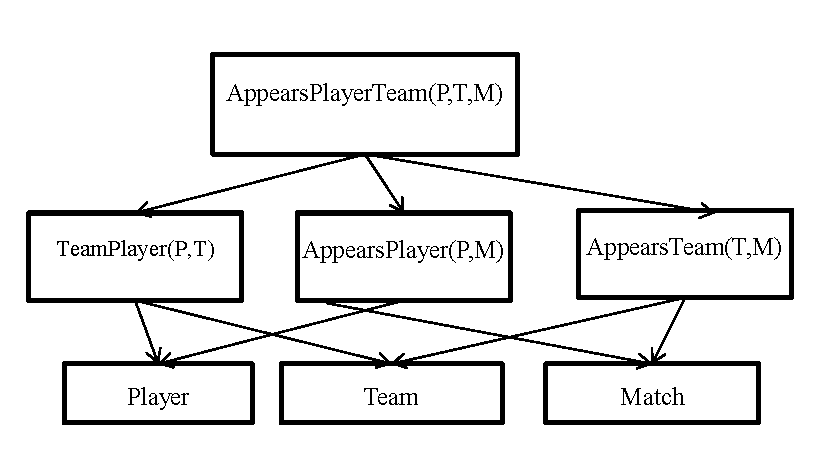
\includegraphics[width=0.3\textwidth] {lattice}
			% \caption{Lattice of Premier League dataset.
			% %We show only the Markov blanket of the Results node to simplify. 
			% \label{fig:lattice}}
			%\end{figure}
			
			
			
			
			%\begin{itemize}
			%\item $\D_{\population}$ is the database for the entire population; cf. Table~\ref{table:data}.
			%\item $\D_{\target}$ is the restriction of the input database to the target object; cf. Table~\ref{table:object}. 
			%\item $\M_{\population}$ is a model (e.g., Bayesian network) learned with $\D_{\population}$ as the input database; cf. Figure~\ref{fig:bns}(a).
			%\item $\M_{\target}$ is an object model (e.g., Bayesian network) learned with $\D_{\target}$ as the input database; cf. Figure~\ref{fig:bns}(b).
			%\end{itemize}
			%
					%consider the parent-child configuration as shown in Figure~\ref{fig:bns}(b). Suppose that the data show that team $\it{WA}$ played 20 matches  in formation 1 with team shot efficiency at level 2 and won 12 of these. Then the maximum likelihood estimate of winning given the parent values is $12/20=0.6.$ The instantiation count is 10, so the instantiation proportion is $10/20 =0.5$. This parent-child configuration contributes $\ln 0.5 \cdot 0.6 = -0.415$ to the aggregate pseudo-likelihood. 
			
			%\section{Class and Object Distributions} 
			
			
			
			%\section{Overview} We describe the object-oriented data model and our approach to defining an object outlier score. In the object-oriented data model, complex objects are composed of simpler objects. This can be visualized as a tree. Objects are associated with attribute values. In this paper we assume that attributes take on discrete values, but this is not essential for our approach. 
			%Figure~\ref{fig:oobn} shows a typical object tree. Matches are complex objects containing a home team and an away team. The match result is a match attribute. Teams are complex objects comprising players. Some player attributes  depend on the context of the match. Players have a special attribute that specifies their class. Note that the same object can appear in different nodes (e.g., Van Persie). 
			%
			%\begin{figure*}[htbp]
			%	\centering
			%	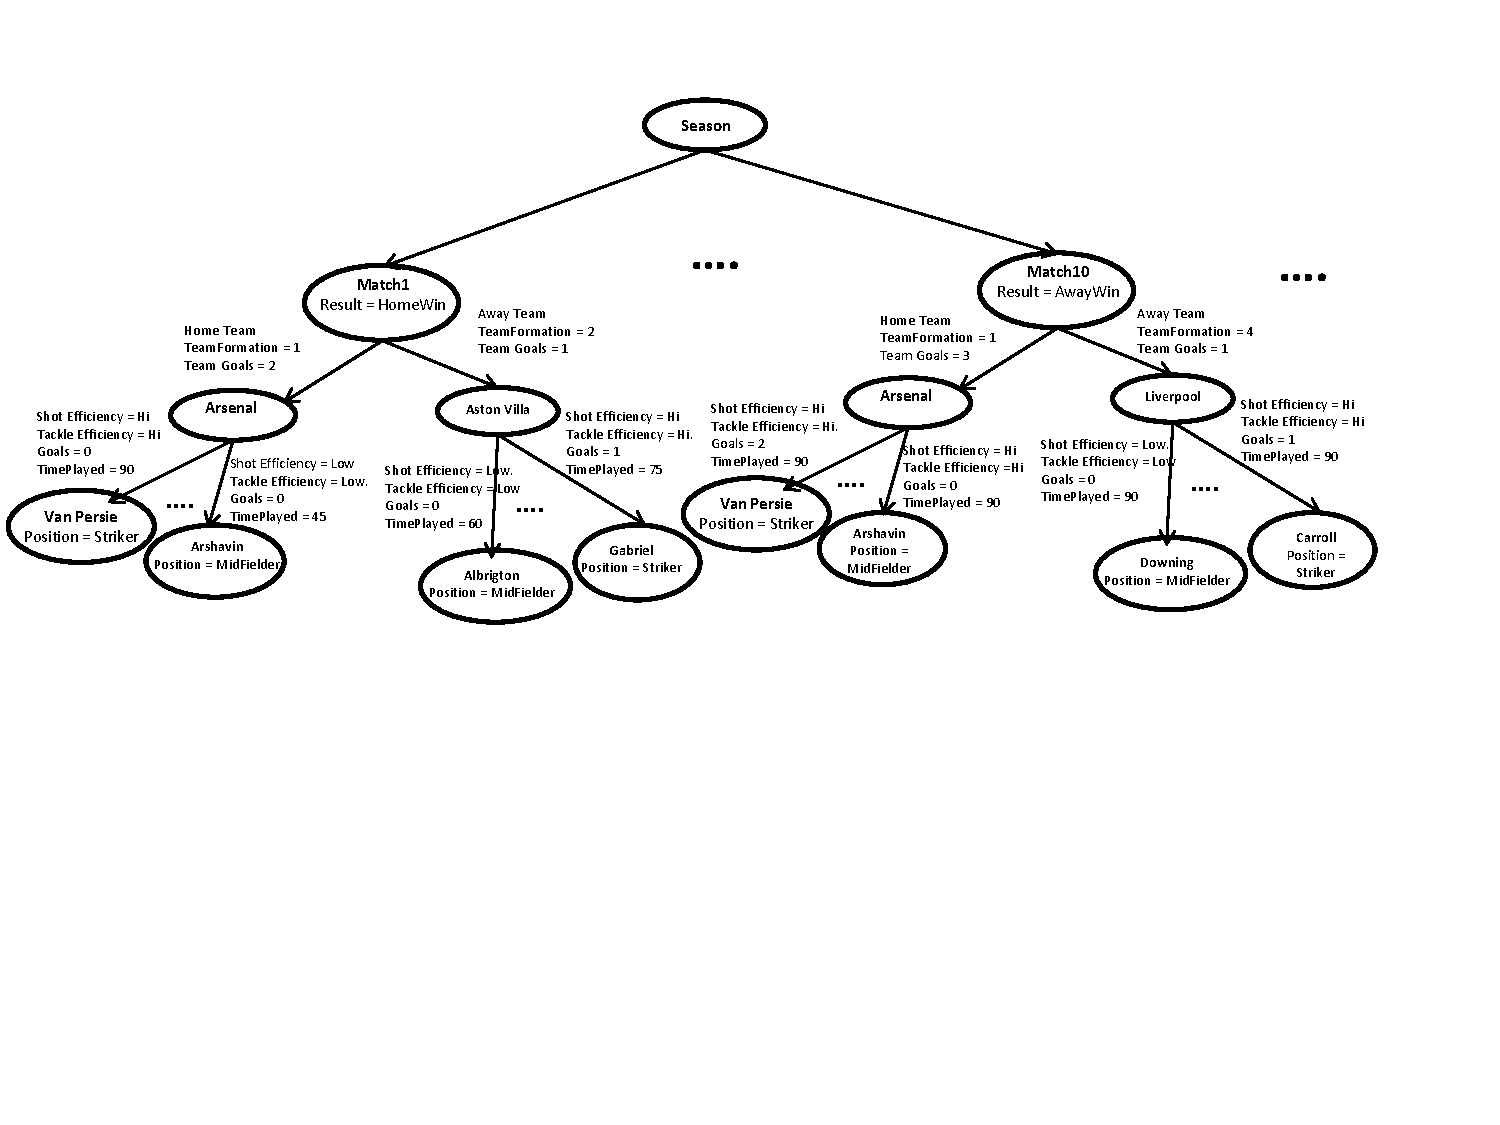
\includegraphics[width=1\textwidth]{SeasonGraph}
			%	\caption{An illustrative object tree. Nodes are labelled with object IDs and object attributes. A season is a complex object comprising matches. A match comprises a home team and an away team. Teams comprise players. Edges go to component objects.  Edge labels indicate the type of component relationship between the linked objects, and attributes associated with this  relationship. 
			%		\label{fig:oobn}}
			%\end{figure*}
			%
			%Our system employs the following steps for outlier detection, illustrated in Figure~\ref{fig:}. 
			%
			%\begin{enumerate}
			%	\item Define a set of path types in the object tree.
			%	\item For a given target object, there is a substructure that contains the other objects linked to the target by paths of the applicable types. We refer to this substructure as the {\em object profile}.
			%	\item For each attribute, the {\em object distribution} counts how many times the attribute occurred in the object's profile. 
			%	\item We define a novel distribution divergence that measures how much the target object's distribution differs from the average distribution of objects in the same class. This divergence is our outlier score.
			%\end{enumerate}
			%
			%In database terminology, an object profile is like a view centered on the object. For example, a query for computing the object profile for Arsenal would include the selection condition $\it{TeamID} = \it{Arsenal}$. Note that an object profile features both parts of the object as well as more complex objects of which it is a part. The object profile is individual-centered in the sense of \cite{Flach1999a}.
			%
			%\begin{figure}[htbp]
			%	\centering
			%	\resizebox{1\textwidth}{!}{
			%		\includegraphics%[width=0.3\textwidth] 
			%		{SystemOverView}
			%	}
			%	\caption{The components in our outlier detection system and the system flow. Aggregation is an alternative to our expected log-distance outlier score.
			%		\label{fig:flow}}
			%\end{figure}
			%
			%\section{Path Types}
			%A path in the tree connects two nodes, with {\em links in either direction}. For example, the object tree contains a path $\it{van Persie} \leftarrow \it{Arsenal} \leftarrow \it{Match1}$ that connects van Persie to the first match of the season. Every path specifies a set of attribute values for the objects and edges contained in the path. 
			%A \textbf{path type} is a set of paths with matching node types and matching edge types. For example, the path $\it{van Persie} \leftarrow \it{Arsenal} \leftarrow \it{Match10}$ is of the same type as the previous one.  For each attribute of a path type, and each value of the attribute, there is a count of the number of times that the attribute value occurs in a path of the type. These counts define the {\em path type distribution.} 
			%%Given a list of path types, we can combine (concatenate) their distributions into a attribute distribution for the list. 
			%%maybe use the term ``metapath''
			%
			%Assume that a list of path types have been fixed. The \textbf{object profile} contains all instances of a type of path that begin with the object. For each type of path, there is a distribution of attribute values over paths of that type in the object profile.
			%The \textbf{object distribution} $P_{\object}$ for object $\object$ combines (concatenates) the path distributions 
			%%over all attributes 
			%in the object profile. 
			%%In order words, it represents the distribution of attribute values over all paths that begin with the object.
			%%a node labelled with the object's ID.
			%The expression $P_{\Class}$ denotes the joint \textbf{class distribution} for the class of object $\object$. This is the joint probability associated with selecting an object uniformly at random from its class. Equivalently, the class distribution can be viewed as the  uniform mixture of object distributions:
			%
			%$$P_{\Class} \equiv \frac{1}{|\Class|} \sum_{\object \in \Class} P_{\object}.$$
			%
			%\paragraph{Example} Suppose we consider only paths of the type $\,$
			%$\it{Player} \leftarrow 
			%\it{Team} \leftarrow \it{Match}$. The attributes of this path type include $\it{Goals},\it{TeamGoals},\it{ShotEfficiency},\it{Result}$. For simplicity only, suppose that the only matches and players in the season are those shown in Figure~\ref{fig:oobn}. Then the attribute value $\it{Goals} = 0$ occurs with frequency $1/2$ in the object distribution $P_{\it{vP}}$ for van Persie. In the player class distribution $P_{\it{Player}}$, the attribute value $\it{Goals} = 0$ occurs with frequency $5/8$. So van Persie is somewhat less likely to score no goal than a randomly selected player.
			%
			%Since our outlier scores are based on the object profiles, they depend on a specification of relevant path types. One option would be to exhaustively include all possible path types. Another is to let a user specify path types of interest, for example all paths of length $k$. In our experiments we use machine learning methods that search the space of path types to find the paths that carry the strongest probabilistic associations between objects (see Section~\ref{sec:bnlearning}  below). 
			
			
			
			%\section{Log-Distance Object Outlier score} \label{sec:metrics}
			%%[There is no bound on the number of objects that a complex object may contain. ]
			%
			%[log distances. Motivation: additive, decomposed, closed form for computation. Relates to baseline methods. Distance not difference: avoid cancelling. Weight by frequency in object domain]
			%
			%Our approach defines an object-oriented outlier score as a {\em model comparison score} of the form 
			%$$\scorediff(\model_{\object},\model_{\Class},\profile_{\object}).$$ Here $\profile_{\object}$ denotes the probability distribution defined by the profile of the potential outlier object $\object$, the symbol $\model_{\object}$ denotes a model of the object profile, and $\model_{\Class}$ denotes a model that represents the normal behavior in the population, learned from the entire dataset. 
			%We use the following notation and definitions to define model comparison scores formally. %
			%%\subsection{Notation and Bayesian Networks}
			%Fix a set of attributes $\Features = \{\feature_{1},\ldots,\feature_{n}\}$. These are attributes of objects, which can and typically do belong to different classes. In statistical terms, each attribute defines a random variable. The possible values of $\feature_{i}$ are enumerated as $\{\nodevalue_{i1},\ldots,\nodevalue_{i\states_{i}}\}$. The notation $P(\feature_{i} = \x)\equiv P(\x)$ denotes the probability of attribute $\feature_{i}$ taking on value $\x$. We also use the vector notation $P(\Features = \set{x}) \equiv P(\set{x})$ to denote the joint probability of that each attribute $\feature_{i}$ takes on value $\set{x}_{i}$. 
			
%In other words, we assume that model comparison scores are decomposable, which is the case for Bayesian networks. 

%\begin{equation} \label{eq:log-dist}
%\begin{array}{l}
%\mid_{i} =\sum_{j=1}^{\states_{i}} P_{\object}(\nodevalue_{ij}) \left|\ln \frac{\parameter_{\object}( \nodevalue_{ij})}{\parameter_{\Class}( \nodevalue_{ij})}\right|+\\
%\sum_{j=1}^{\states_{i}} \sum_{\parents_{i}} 
%P_{\object}( \nodevalue_{ij},\parents_{i})
%\left|\ln \frac{\parameter_{\object}( \nodevalue_{ij}|\parents_{i})}{\parameter_{\object}(\nodevalue_{ij})} - \ln \frac{\parameter_{\Class}( \nodevalue_{ij}|\parents_{i})}{\parameter_{\Class}(\nodevalue_{ij})}\right|. 
%\end{array}
%\end{equation}
%We note that for a fixed object distribution $P_{\object}$, the log-likelihood distance is a proper distance metric between the class-level and the object-level parameters. 
%The $\mid$ has two components. 


\subsection{Motivation} 
%The motivation for using log-distances %rather than log-differences 
%is that some log-differences are positive, some negative, and cancel each other out when their sign differs. Since our goal is to assess the distinctness of an object, {\em we do not want differences to cancel out.} Fundamentally, averaging differences is appropriate when considering costs, payoffs or utilities, but not appropriate when assessing the distinctness of an object. 
%
The motivation for the mutual information decomposition is two-fold. 

\noindent
(1) {\em Interpretability.} This is very important for outlier detection. The single-feature components are easy to interpret since they involve no feature interactions. Each parent-child local factor is based on the average relevance of parent values for predicting the value of the child node, where relevance is measured by $$\ln \frac{\parameter(\nodevalue_{ij}|\parents_{i})}{\parameter(\nodevalue_{ij})}.$$ This relevance term  is basically the same as the widely used lift measure \cite{Tuffery2011}, and therefore is an intuitively meaningful quantity. The $\mid$ score compares how relevant a given parent condition is in the object data with how relevant it is in the general class. 

\noindent
(2) {\em Avoiding cancellations.} The \textbf{mutual information decomposition} shows that each term in the log-likelihood difference \eqref{eq:log-diff} decomposes into a relevance difference and a marginal difference: 

\begin{equation} \label{eq:decompose}
\ln \frac{\parameter_{\object}( \nodevalue_{ij}|\parents_{i})}{\parameter_{\Class}( \nodevalue_{ij}|\parents_{i})} = \ln \frac{\parameter_{\object}(\nodevalue_{ij}|\parents_{i})}{\parameter_{\object}(\nodevalue_{ij})} - \ln \frac{\parameter_{\Class}( \nodevalue_{ij}|\parents_{i})}{\parameter_{\Class}(\nodevalue_{ij})} + \ln \frac{\parameter_{\object}( \nodevalue_{ij})}{\parameter_{\Class}( \nodevalue_{ij})}.
\end{equation}

These differences can have different signs for different child-parent configurations and cancel each other out; see Table~\ref{table:example} below for an example.  Since our goal is to assess the distinctness of an object, {\em we do not want differences to cancel out.} Taking distances as in Equations~\eqref{eq:fd} and ~\eqref{eq:mi} avoids the undesirable cancellation. The general point is that averaging differences is appropriate when considering costs, or utilities, but not appropriate for assessing the distinctness of an object. For instance, the average component-wise difference of the vectors (0,0) and (1,-1) is 0, but their distance is not.


%
%\subsection{Comparison Outlier Scores} \label{sec:comparison} Our lesion study compares our log-likelihood distance  $\mid$ score to baselines that are defined by omitting a component of $\mid$. In this section we define these scores.
%%and provide a theoretical comparison. 
%The scores increase in sophistication in the sense that they apply more transformations of the log-likelihood ratio. 
%%Our empirical comparison below indicates that the 
%More sophisticated scores provide more information about outliers.   
%%defines the scores formally.  
%Table~\ref{table:Formula} defines local feature scores; the total score is the sum of feature-wise scores. All metrics are defined such that {\em a higher score indicates a greater anomaly.} The metrics are as follows. 
%
%\begin{description}
%	\item[Feature Divergence $\fd$] is the first  component of the $\mid$ score. It considers each feature independently (no feature correlations).
%	%							
%	\item[Log-Likelihood Score \loglikelihood] is the standard model-based outlier detection score using data likelihood.
%	\item[Log-Likelihood Difference \lr] is the log-likelihood difference~\eqref{eq:log-diff} between the class-level and object-level parameters. %(Equation). 
%	\item[Log-Likelihood Difference with absolute value $|\lr|$] replaces differences in $\lr$ by distances.
%	\item[Log-Likelihood Difference with decomposition $\lr^{+}$] applies a mutual information decomposition to $\lr$.
%\end{description}
%
%
%
%\begin{table}
%	\caption{Baseline Comparison Outlier Scores % for Bayesian Networks
%		\label{table:Formula}}
%	\resizebox{1\textwidth}{!}{
%		\begin{tabular}{|l|l|} \hline
%			Method & Formula\\
%			\hline
%			
%			$\fd_{i}	$&	$\begin{array}{l}\sum_{i=1}^{n}\sum_{j=1}^{\states_{i}} P_{\object}( \nodevalue_{ij}) \left|\ln \frac{\parameter_{\object}( \nodevalue_{ij})}{\parameter_{\Class}( \nodevalue_{ij})}\right|\end{array}	$\\ \hline
%			
%			$-\loglikelihood_{i}$& $  \begin{array}{l} -\sum_{i=1}^{n}\sum_{j=1}^{\states_{i}} \sum_{\parents_{i}} P_{\object}( \nodevalue_{ij},\parents_{i})\ln \parameter_{\Class}( \nodevalue_{ij}|\parents_{i})\end{array}$ \\ \hline
%			$\lr_{i}$&$\begin{array}{l}  \sum_{j=1}^{\states_{i}} \sum_{\parents_{i}} P_{\object}( \nodevalue_{ij},\parents_{i})\ln \frac{\theta_{\object}(  \nodevalue_{ij}|\parents_{i})}{\theta_{\Class}( \nodevalue_{ij}|\parents_{i})}.  \end{array}$\\	\hline
%			$|\lr_{i}|$& $\begin{array}{l}  \sum_{j=1}^{\states_{i}} \sum_{\parents_{i}} P_{\object}( \nodevalue_{ij},\parents_{i})|\ln \frac{\theta_{\object}(\nodevalue_{ij}|\parents_{i})}{\theta_{\Class}( \nodevalue_{ij}|\parents_{i})}|. \end{array}$ \\	\hline
%			$\lr_{i}^{+}$&$\begin{array}{l}  \sum_{j=1}^{\states_{i}} P_{\object}( \nodevalue_{ij}) \ln \frac{\parameter_{\object}( \nodevalue_{ij})}{\parameter_{\Class}( \nodevalue_{ij})}+
%			\\ \sum_{j=1}^{\states_{i}} \sum_{\parents_{i}} 
%			P_{\object}( \nodevalue_{ij},\parents_{i})
%			\ln \frac{\theta_{\object}( \nodevalue_{ij}|\parents_{i})}{\parameter_{\object}(\nodevalue_{ij})} - \ln \frac{\theta_{\Class}( \nodevalue_{ij}|\parents_{i})}{\parameter_{\Class}(\nodevalue_{ij})}.  \end{array}$ \\ \hline
%			
%		\end{tabular} 
%	}
%\end{table}
%
%
%The next proposition shows that the outlier scores have the standard properties of a divergence measure between probability distributions: they are nonnegative, and 0 if and only if the class and object distributions are the same. Also, the triangle inequality entails that the scores can be ordered by {\em dominance:} one is guaranteed to be at least as great as another. Dominance means that a divergence potentially provides more discrimination among objects as it maps the set of objects onto a larger range of scores. Our $\mid$ score dominates all others.  We provide empirical evidence that dominance leads to greater discrimination.

%\begin{proposition} \label{prop:divergence} The following hold for any class and object distributions, and each node $\node_{i}$.
%
%\begin{enumerate}
%\item For any class and object distribution, we have $\mid_{i} \geq |\lr_{i}| \geq \lr_{i} = \lr_{i}^{+} \geq 0$. Also, $\mid_{i} \geq \fd_{i}$. \label{clause:inequalities}
%\item All divergences $\mid_{i},|\lr_{i}|,\lr_{i},\lr_{i}^{+},\fd_{i}$ are nonnegative. The divergences are 0 if and only if the object parameters $\parameters_{\object}$ and class parameters $\parameters_{\Class}$ are the same. \label{clause:nonnegative}
%\end{enumerate}
%These properties also hold for the divergences $\mid,|\lr|,\lr,\lr^{+},\fd$ summed over all nodes.
%\end{proposition}
%\begin{proof}
%(Part \ref{clause:inequalities}) It is immediate that $\mid_{i} \geq \fd_{i}$. We show that $\lr = \lr^{+} $. Using the marginalization
%
%\begin{equation} \label{eq:marginalize}
%P_{\object}( \nodevalue_{ij}) \ln \frac{\parameter_{\object}( \nodevalue_{ij})}{\parameter_{\Class}( \nodevalue_{ij})} = \sum_{\parents_{i}} 
%			P_{\object}( \nodevalue_{ij},\parents_{i}) \ln \frac{\parameter_{\object}( \nodevalue_{ij})}{\parameter_{\Class}( \nodevalue_{ij})} 
%\end{equation}


%\begin{eqnarray} 
%P_{\object}( \nodevalue_{ij}) \ln \frac{\parameter_{\object}( \nodevalue_{ij})}{\parameter_{\Class}( \nodevalue_{ij})} & = & \sum_{\parents_{i}} 
%			P_{\object}( \nodevalue_{ij},\parents_{i}) \ln \frac{\parameter_{\object}( \nodevalue_{ij})}{\parameter_{\Class}( \nodevalue_{ij})} \\
%\ln \theta_{\object}(  \nodevalue_{ij}|\parents_{i})- \ln\theta_{\Class}( \nodevalue_{ij}|\parents_{i})	&=&		\ln \frac{\parameter_{\object}( \nodevalue_{ij})}{\parameter_{\Class}( \nodevalue_{ij})} +
%			\ln \frac{\theta_{\object}( \nodevalue_{ij}|\parents_{i})}{\parameter_{\object}(\nodevalue_{ij})} - \ln \frac{\theta_{\Class}( \nodevalue_{ij}|\parents_{i})}{\parameter_{\Class}(\nodevalue_{ij})} \label{eq:decompose}
%\end{eqnarray}
%and the mutual information decomposition~\eqref{eq:decompose}
%it is easy to verify that $\lr_{i}^{+}$ simplies to $\lr$. Next, $|\lr_{i}| \geq \lr_{i}$ holds because $a-b \leq |a-b|$ for any numbers $a,b$. The inequality $\mid_{i} \geq |\lr_{i}|$ is established as follows.

%\begin{eqnarray*}
%\lr_{i}^{+} & = & \sum_{j=1}^{\states_{i}} \sum_{\parents_{i}} 
%			P_{\object}( \nodevalue_{ij},\parents_{i}) \ln \frac{\parameter_{\object}( \nodevalue_{ij})}{\parameter_{\Class}( \nodevalue_{ij})} + 
%			\sum_{j=1}^{\states_{i}} \sum_{\parents_{i}} 
%			P_{\object}( \nodevalue_{ij},\parents_{i})
%			\left( \ln \frac{\theta_{\object}( \nodevalue_{ij}|\parents_{i})}{\parameter_{\object}(\nodevalue_{ij})} - \ln \frac{\theta_{\Class}( \nodevalue_{ij}|\parents_{i})}{\parameter_{\Class}(\nodevalue_{ij})}\right)\\
%			& = & \sum_{j=1}^{\states_{i}} \sum_{\parents_{i}} 
%			P_{\object}( \nodevalue_{ij},\parents_{i})
%			\left(\ln \frac{\parameter_{\object}( \nodevalue_{ij})}{\parameter_{\Class}( \nodevalue_{ij})} +
%			\ln \frac{\theta_{\object}( \nodevalue_{ij}|\parents_{i})}{\parameter_{\object}(\nodevalue_{ij})} - \ln \frac{\theta_{\Class}( \nodevalue_{ij}|\parents_{i})}{\parameter_{\Class}(\nodevalue_{ij})} \right) \\
%			& = & \sum_{j=1}^{\states_{i}} \sum_{\parents_{i}} P_{\object}( \nodevalue_{ij},\parents_{i})\left( \ln \theta_{\object}(  \nodevalue_{ij}|\parents_{i})- \ln\theta_{\Class}( \nodevalue_{ij}|\parents_{i}) \right) \\
%			& = & \lr_{i}
%\end{eqnarray*}


%
%\begin{eqnarray}
%\notag \mid & = & \sum_{j=1}^{\states_{i}} \sum_{\parents_{i}} 
%			P_{\object}( \nodevalue_{ij},\parents_{i}) \left|\ln \frac{\parameter_{\object}( \nodevalue_{ij})}{\parameter_{\Class}( \nodevalue_{ij})} \right| + 
%			\sum_{j=1}^{\states_{i}} \sum_{\parents_{i}} 
%			P_{\object}( \nodevalue_{ij},\parents_{i})
%			\left| \ln \frac{\theta_{\object}( \nodevalue_{ij}|\parents_{i})}{\parameter_{\object}(\nodevalue_{ij})} - \ln \frac{\theta_{\Class}( \nodevalue_{ij}|\parents_{i})}{\parameter_{\Class}(\nodevalue_{ij})}\right|\\ 
%			& = & \sum_{j=1}^{\states_{i}} \sum_{\parents_{i}} 
%			P_{\object}( \nodevalue_{ij},\parents_{i})
%			\left|\ln \frac{\parameter_{\object}( \nodevalue_{ij})}{\parameter_{\Class}( \nodevalue_{ij})}\right| +
%			\left|\ln \frac{\theta_{\object}( \nodevalue_{ij}|\parents_{i})}{\parameter_{\object}(\nodevalue_{ij})} - \ln \frac{\theta_{\Class}( \nodevalue_{ij}|\parents_{i})}{\parameter_{\Class}(\nodevalue_{ij})} \right| \label{eq:marginal2} \\
%			& \geq & \sum_{j=1}^{\states_{i}} \sum_{\parents_{i}} 
%			P_{\object}( \nodevalue_{ij},\parents_{i})
%			\left|\ln \frac{\parameter_{\object}( \nodevalue_{ij})}{\parameter_{\Class}( \nodevalue_{ij})} +
%			\ln \frac{\theta_{\object}( \nodevalue_{ij}|\parents_{i})}{\parameter_{\object}(\nodevalue_{ij})} - \ln \frac{\theta_{\Class}( \nodevalue_{ij}|\parents_{i})}{\parameter_{\Class}(\nodevalue_{ij})} \right| \label{eq:triangle} \\
%			& = & \sum_{j=1}^{\states_{i}} \sum_{\parents_{i}} P_{\object}( \nodevalue_{ij},\parents_{i})\left| \ln \theta_{\object}(  \nodevalue_{ij}|\parents_{i})- \ln\theta_{\Class}( \nodevalue_{ij}|\parents_{i}) \right| \label{eq:decompose2} \\
%			& = &|\lr_{i}|
%\end{eqnarray}
%
%Here Equation~\eqref{eq:marginal2} follows from Equation~\eqref{eq:marginalize}, inequality~\ref{eq:triangle} follows from the triangle inequality $|a|+|b|\geq |a+b|$, and Equation~\eqref{eq:decompose2} from Equation~\eqref{eq:decompose}.
%
%(Part \ref{clause:nonnegative}) The claim is immediate for $\fd_{i}$. We show that $\lr_{i}$ is nonnegative and 0 only if the object and class parameters associated with node $i$ are the same. 
%%We apply the well-known fact that the KL-divergence of two distributions is nonnegative and 0 only if the two distributions are the same. 
%Consider a simple Bayes net structure $\model'$ comprising the parents of node $i$, node $i$, and no other nodes or links. Then $\lr_{i}$ is the log-likelihood difference $$ \lr_{i} =\loglikelihood(\D_{\object},\model',\parameters_{\object}) - \loglikelihood(\D_{\object},\model',\parameters_{\Class}).$$ The empirical frequency parameters $\parameters_{\object}$ uniquely maximize the function $\loglikelihood(\D_{\object},\model',\cdot)$ \cite{Schulte2012}, so the difference $\lr_{i}$ is nonnegative, and equals 0 if and only if $\theta_{\Class} = \theta_{\parameters}$.
%\end{proof}

%Let $P_{\Class'}$ be a distribution that agrees with $P_{\object}$ on the marginal probabilities over the parent nodes, and agrees with $P_{\Class}$ on the conditional probabilities of the child node given parent values (i.e. $\parameters_{\Class'} = \parameters_{\Class}$). Then $\lr_{i}$ is the KL-divergence between the two distributions $P(\cdot;\model',\parameters_{\Class'})$ and $P(\cdot;\model',\parameters_{\object})$. Therefore $\lr_{i}$ is nonnegative and 0 only if $\parameters_{\object} = \parameters_{\Class'} = \parameters_{\Class}$. The nonnegativity of the other divergences now follows from the equality and inequalities established in part \ref{clause:inequalities}.



